\documentclass[11pt,a4paper]{article}

% ==================== TEMEL PAKETLER (pdflatex) ====================
\usepackage[T1]{fontenc}
\usepackage[utf8]{inputenc}
\usepackage{lmodern}
\usepackage[a4paper,margin=2cm,top=2.4cm,bottom=2.4cm]{geometry}
\usepackage{xcolor}
\usepackage{colortbl}
\usepackage{array}
\usepackage{booktabs}
\usepackage{longtable}
\usepackage{tabularx}
\usepackage{listings}
\usepackage{fancyhdr}
\usepackage{amsmath}
\usepackage{amssymb}
\usepackage{tikz}
\usetikzlibrary{arrows.meta,calc,positioning,patterns}
\usepackage{hyperref}

% ==================== RENK PALETİ ====================
\definecolor{anaMavi}{HTML}{1B3A5B}
\definecolor{vurguMavi}{HTML}{2E6DA4}
\definecolor{acikMavi}{HTML}{EAF2F9}
\definecolor{turuncu}{HTML}{D9701E}
\definecolor{yesil}{HTML}{2E7D32}
\definecolor{acikYesil}{HTML}{E8F5E9}
\definecolor{kirmizi}{HTML}{C0392B}
\definecolor{mor}{HTML}{6C3483}
\definecolor{acikMor}{HTML}{F3E9F7}
\definecolor{acikGri}{HTML}{F4F5F7}
\definecolor{ortaGri}{HTML}{6B7280}
\definecolor{koyuGri}{HTML}{2D2D2D}
\definecolor{kodArka}{HTML}{FBFBFA}
\definecolor{grafikMavi}{HTML}{2E6DA4}
\definecolor{petrol}{HTML}{0E6E7C}
\definecolor{acikPetrol}{HTML}{E4F2F4}
\definecolor{amber}{HTML}{9C6407}
\definecolor{acikAmber}{HTML}{FDF4E0}

% ==================== HYPERREF ====================
\hypersetup{
  colorlinks=true,
  linkcolor={[HTML]{2E6DA4}},
  urlcolor={[HTML]{2E6DA4}},
  pdftitle={Python ile İstatistik, Olasılık ve Makine Öğrenmesi},
  pdfauthor={Veri Bilimi Rehberi},
  bookmarksnumbered=true
}

% ==================== BAŞLIK STİLLERİ ====================
\setcounter{secnumdepth}{0}
\newcounter{secc}
\newcounter{subsecc}[secc]
\newcounter{subsubsecc}[subsecc]
\newcommand{\gsec}[1]{\par\phantomsection\stepcounter{secc}%
  \setcounter{subsecc}{0}%
  \vspace{18pt}{\color{anaMavi}\Large\bfseries\thesecc.\hspace{0.5em}#1}\par
  \vspace{2pt}{\color{turuncu}\rule{\linewidth}{1.6pt}}\par\vspace{8pt}%
  \addcontentsline{toc}{section}{\protect\numberline{\thesecc}#1}\markboth{#1}{#1}}
\newcommand{\gsub}[1]{\par\phantomsection\stepcounter{subsecc}%
  \setcounter{subsubsecc}{0}%
  \vspace{11pt}{\color{vurguMavi}\large\bfseries\thesecc.\thesubsecc\hspace{0.5em}#1}\par\vspace{4pt}%
  \addcontentsline{toc}{subsection}{\protect\numberline{\thesecc.\thesubsecc}#1}}
\newcommand{\gsubsub}[1]{\par\vspace{7pt}{\color{koyuGri}\normalsize\bfseries #1}\par\vspace{2pt}}

% Kısım (Part) başlığı
\newcommand{\gpart}[2]{\clearpage
  \begin{center}\vspace*{1.5cm}
  {\color{turuncu}\rule{0.7\linewidth}{1.5pt}}\\[10pt]
  {\color{ortaGri}\Large KISIM #1}\\[8pt]
  {\color{anaMavi}\Huge\bfseries #2}\\[10pt]
  {\color{turuncu}\rule{0.7\linewidth}{1.5pt}}
  \end{center}\vspace{1cm}}

% ==================== BAŞLIK / ALTBİLGİ ====================
\setlength{\headheight}{14pt}
\pagestyle{fancy}
\fancyhf{}
\renewcommand{\headrulewidth}{0.4pt}
\renewcommand{\footrulewidth}{0.4pt}
\fancyhead[L]{\small\color{ortaGri}İstatistik, Olasılık ve Makine Öğrenmesi}
\fancyhead[R]{\small\color{ortaGri}\leftmark}
\fancyfoot[C]{\small\color{ortaGri}\thepage}

% ==================== KOD LİSTELEME (Python) ====================
\lstdefinestyle{pystyle}{
  language=Python,
  basicstyle=\ttfamily\small\color{koyuGri},
  keywordstyle=\color{vurguMavi}\bfseries,
  commentstyle=\color{yesil}\itshape,
  stringstyle=\color{turuncu},
  numberstyle=\tiny\color{ortaGri},
  numbers=left,
  numbersep=8pt,
  backgroundcolor=\color{kodArka},
  frame=single,
  framesep=6pt,
  rulecolor=\color{ortaGri!40},
  breaklines=true,
  showstringspaces=false,
  tabsize=4,
  columns=fullflexible,
  keepspaces=true,
  extendedchars=true,
  literate={ı}{{\i}}1{İ}{{\.I}}1{ş}{{\c s}}1{Ş}{{\c S}}1{ğ}{{\u g}}1{Ğ}{{\u G}}1{ç}{{\c c}}1{Ç}{{\c C}}1{ö}{{\"o}}1{Ö}{{\"O}}1{ü}{{\"u}}1{Ü}{{\"U}}1,
  morekeywords={np,pd,plt,sns,sm,smf,st,as,with,yield,lambda,None,True,False,
    self,assert,DataFrame,Series,fit,transform,predict,fit_transform,
    train_test_split,cross_val_score,GridSearchCV,Pipeline,StandardScaler,
    LogisticRegression,RandomForestClassifier,accuracy_score,roc_auc_score}
}
\lstset{style=pystyle}

% Kabuk/terminal stili
\lstdefinestyle{shstyle}{
  numbers=none,
  basicstyle=\ttfamily\small\color{koyuGri},
  backgroundcolor=\color{koyuGri!6},
  frame=single,framesep=6pt,rulecolor=\color{ortaGri!40},
  breaklines=true,showstringspaces=false,tabsize=4,columns=fullflexible,
  keepspaces=true,
  literate={ı}{{\i}}1{İ}{{\.I}}1{ş}{{\c s}}1{Ş}{{\c S}}1{ğ}{{\u g}}1{Ğ}{{\u G}}1{ç}{{\c c}}1{Ç}{{\c C}}1{ö}{{\"o}}1{Ö}{{\"O}}1{ü}{{\"u}}1{Ü}{{\"U}}1,
}

% Program çıktısı stili
\lstdefinestyle{outstyle}{
  numbers=none,
  basicstyle=\ttfamily\footnotesize\color{anaMavi},
  backgroundcolor=\color{acikMavi},
  frame=single,framesep=6pt,rulecolor=\color{vurguMavi!40},
  breaklines=true,showstringspaces=false,tabsize=4,columns=fullflexible,
  keepspaces=true,
  literate={ı}{{\i}}1{İ}{{\.I}}1{ş}{{\c s}}1{Ş}{{\c S}}1{ğ}{{\u g}}1{Ğ}{{\u G}}1{ç}{{\c c}}1{Ç}{{\c C}}1{ö}{{\"o}}1{Ö}{{\"O}}1{ü}{{\"u}}1{Ü}{{\"U}}1,
}

% ==================== ÖZEL KUTULAR ====================
\newcommand{\callout}[4]{\par\smallskip\noindent\begingroup
  \setlength{\fboxsep}{8pt}\setlength{\fboxrule}{0.8pt}%
  \fcolorbox{#1}{#2}{\parbox{\dimexpr\linewidth-2\fboxsep-2\fboxrule\relax}{%
    {\bfseries\color{#1}#3}\par\smallskip #4}}\endgroup\par\smallskip}
\newcommand{\bilgi}[1]{\callout{vurguMavi}{acikMavi}{Bilgi}{#1}}
\newcommand{\ipucu}[1]{\callout{yesil}{acikYesil}{İpucu}{#1}}
\newcommand{\uyari}[1]{\callout{kirmizi}{kirmizi!7}{Dikkat}{#1}}
\newcommand{\tanim}[2][Tanım]{\callout{vurguMavi}{acikMavi}{#1}{#2}}
\newcommand{\form}[2][Formül]{\callout{mor}{acikMor}{#1}{#2}}
\newcommand{\teorem}[2][Teorem]{\callout{mor}{acikMor}{#1}{#2}}
\newcommand{\notk}[2][Not]{\callout{mor}{acikMor}{#1}{#2}}
\newcommand{\ornek}[2][Örnek]{\callout{ortaGri!90!black}{acikGri}{#1}{#2}}
\newcommand{\veri}[2][Gerçek Veri]{\callout{turuncu}{turuncu!7}{#1}{#2}}
% Nedir? Nicin? Nerede? --- her formulun ardindan gelen aciklama kutusu
\newcommand{\nicin}[2][Nedir? Niçin? Nerede?]{\callout{petrol}{acikPetrol}{#1}{#2}}
% Gercek hayattan somut hikaye
\newcommand{\gercek}[2][Gerçek Hayattan]{\callout{amber}{acikAmber}{#1}{#2}}
% Sezgi: formulu kelimelerle okumak
\newcommand{\sezgi}[2][Sezgi]{\callout{petrol}{acikPetrol}{#1}{#2}}

% Soru / Çözüm
\newcounter{soruc}
\newcommand{\soru}[1]{\par\smallskip\refstepcounter{soruc}%
  \noindent\begingroup\setlength{\fboxsep}{8pt}\setlength{\fboxrule}{0.8pt}%
  \fcolorbox{turuncu}{turuncu!6}{\parbox{\dimexpr\linewidth-2\fboxsep-2\fboxrule\relax}{%
  {\bfseries\color{turuncu}Soru \thesoruc}\par\smallskip #1}}\endgroup\par\smallskip}
\newcommand{\cozum}{\par\noindent{\bfseries\color{yesil}Çözüm.}\ }

% Yardımcı komutlar
\newcommand{\code}[1]{\texttt{\color{koyuGri}#1}}
\renewcommand{\arraystretch}{1.35}
\newcommand{\dd}{\,\mathrm{d}}
\newcommand{\E}{\mathbb{E}}
\newcommand{\Var}{\operatorname{Var}}
\newcommand{\Cov}{\operatorname{Cov}}
\newcommand{\Prob}{\mathbb{P}}
\newcommand{\iid}{\overset{\text{iid}}{\sim}}

% ==================== BAŞLANGIÇ ====================
\begin{document}

% ---------- KAPAK ----------
\begin{titlepage}
\centering
\vspace*{0.4cm}
{\color{turuncu}\rule{\textwidth}{2pt}}\\[8pt]
{\color{anaMavi}\Huge\bfseries İstatistik, Olasılık ve\\[6pt] Makine Öğrenmesi}\\[10pt]
{\color{vurguMavi}\LARGE Python ile Kapsamlı Ders Dokümanı}\\[8pt]
{\color{ortaGri}\large Gerçek Veri Setleriyle, Teoriden Uçtan Uca Projelere}\\[6pt]
{\color{turuncu}\rule{\textwidth}{2pt}}\\[0.8cm]

\begin{center}
\fcolorbox{vurguMavi}{acikMavi}{\parbox{0.88\textwidth}{\centering\large
Bu belge üç konuyu tek bir zincir olarak anlatır: \textbf{olasılık}
belirsizliğin dilidir, \textbf{istatistik} veriden çıkarım yapmanın yöntemidir,
\textbf{makine öğrenmesi} ise bu çıkarımı otomatikleştiren mühendisliktir. Her
kavram önce sezgisel, sonra matematiksel olarak verilir; ardından
\textbf{gerçek veri setleri} üzerinde Python'la uygulanır --- çıktılarıyla
birlikte.\vspace{4pt}

\textbf{Hiçbir formül açıklamasız bırakılmamıştır.} Her denklemin ardından
\emph{o denklem nedir, niçin böyle kurulmuştur, hangi soruyu cevaplar ve
gerçek hayatta nerede kullanılır} sorularını yanıtlayan bir açıklama kutusu
ve konuyu somutlaştıran gerçek hayat örnekleri gelir.\vspace{4pt}}}
\end{center}

\vspace{0.45cm}
\begin{center}
\fcolorbox{ortaGri!50}{acikGri}{\parbox{0.88\textwidth}{\footnotesize
\textbf{Kısım 1 --- Araç Kutusu:} NumPy/pandas \textbullet\ gerçek veri
setlerini yükleme \textbullet\ keşifsel veri analizi \textbullet\ eksik veri
\textbullet\ veri tipleri ve ölçek düzeyleri.\vspace{2pt}

\textbf{Kısım 2 --- Betimsel İstatistik:} merkezî eğilim \textbullet\ yayılım
\textbullet\ çeyrekler \& aykırı değerler \textbullet\ çarpıklık/basıklık
\textbullet\ korelasyon \textbullet\ görselleştirme \textbullet\ Simpson
paradoksu.\vspace{2pt}

\textbf{Kısım 3 --- Olasılık:} aksiyomlar \textbullet\ koşullu olasılık
\textbullet\ Bayes teoremi \textbullet\ kombinatorik \textbullet\ rastgele
değişkenler \textbullet\ beklenen değer \& varyans \textbullet\ eşbileşik
dağılımlar.\vspace{2pt}

\textbf{Kısım 4 --- Dağılımlar:} Bernoulli, binom, Poisson, geometrik,
hipergeometrik \textbullet\ normal, üstel, gamma, beta, $t$, $\chi^2$, $F$
\textbullet\ BSY \& Merkezi Limit Teoremi \textbullet\ Monte Carlo.\vspace{2pt}

\textbf{Kısım 5 --- Çıkarım:} örnekleme dağılımları \textbullet\ MLE \&
momentler yöntemi \textbullet\ yanlılık-varyans \textbullet\ güven aralıkları
\textbullet\ bootstrap.\vspace{2pt}

\textbf{Kısım 6 --- Hipotez Testleri:} $p$-değeri \textbullet\ $t$-testleri
\textbullet\ ANOVA \textbullet\ $\chi^2$ \textbullet\ parametrik olmayan
testler \textbullet\ permütasyon \textbullet\ güç analizi \textbullet\ çoklu
karşılaştırma \textbullet\ Bayesçi çıkarım.\vspace{2pt}

\textbf{Kısım 7 --- Regresyon:} OLS türetimi \textbullet\ \code{statsmodels}
çıktısını okuma \textbullet\ varsayım tanıları \textbullet\ VIF \textbullet\
lojistik \& Poisson regresyon \textbullet\ Ridge/Lasso.\vspace{2pt}

\textbf{Kısım 8 --- ML Temelleri:} eğitim/test \textbullet\ çapraz doğrulama
\textbullet\ veri sızıntısı \textbullet\ yanlılık-varyans \textbullet\
\code{Pipeline} \textbullet\ ön işleme \textbullet\ metrikler.\vspace{2pt}

\textbf{Kısım 9 --- Denetimli Öğrenme:} $k$-NN \textbullet\ Naive Bayes
\textbullet\ SVM \textbullet\ karar ağaçları \textbullet\ Random Forest
\textbullet\ Gradient Boosting \textbullet\ stacking \textbullet\
hiperparametre ayarı.\vspace{2pt}

\textbf{Kısım 10 --- Denetimsiz Öğrenme:} K-Means \textbullet\ hiyerarşik
kümeleme \textbullet\ DBSCAN \textbullet\ GMM \textbullet\ PCA \textbullet\
t-SNE \textbullet\ anomali tespiti.\vspace{2pt}

\textbf{Kısım 11 --- İleri Konular:} dengesiz veri \textbullet\ model
yorumlama (permütasyon önemi, SHAP, PDP) \textbullet\ kalibrasyon
\textbullet\ zaman serileri \textbullet\ sinir ağları.\vspace{2pt}

\textbf{Kısım 12 --- Projeler:} Titanic \textbullet\ California Housing
\textbullet\ Breast Cancer \textbullet\ müşteri segmentasyonu \textbullet\
A/B testi.\vspace{2pt}

\textbf{Kısım 13 --- Referans:} dağılım tablosu \textbullet\ test seçme akışı
\textbullet\ scikit-learn sözlüğü \textbullet\ sık yapılan hatalar.\vspace{2pt}}}
\end{center}

\vfill
{\color{ortaGri}\large Hazırlanma Tarihi: 9 Eylül 2026}\\[4pt]
{\color{ortaGri} Anlatım Türkçe \textbullet\ Kod ve terimler İngilizce \textbullet\ Tüm çıktılar gerçek çalıştırmalardan}
\vspace*{0.3cm}
\end{titlepage}

% ---------- İÇİNDEKİLER ----------
\tableofcontents
\thispagestyle{empty}
\clearpage

% #####################################################################
\gpart{1}{Araç Kutusu ve Gerçek Veri Setleri}
% #####################################################################

% =====================================================================
\gsec{Bu Rehber Nasıl Okunur?}
% =====================================================================

Üç konu birbirinin devamıdır ve bu sırayla öğrenilmelidir:

\begin{center}
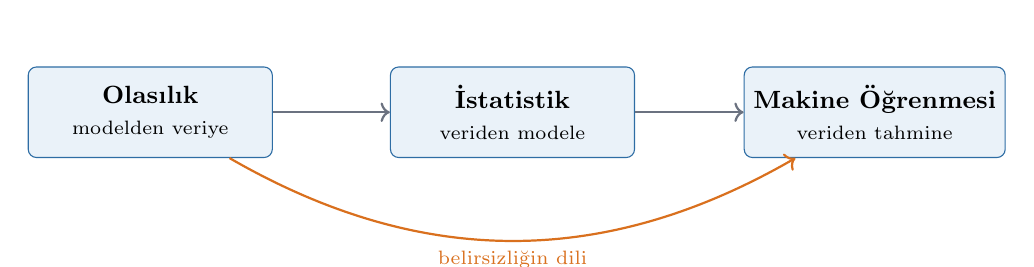
\begin{tikzpicture}[scale=1.0, every node/.style={font=\small},
  kutu/.style={draw=vurguMavi,fill=acikMavi,rounded corners=3pt,
               minimum width=3.1cm,minimum height=1.15cm,align=center}]
\node[kutu] (o) at (0,0) {\textbf{Olasılık}\\ \scriptsize modelden veriye};
\node[kutu] (i) at (4.6,0) {\textbf{İstatistik}\\ \scriptsize veriden modele};
\node[kutu] (m) at (9.2,0) {\textbf{Makine Öğrenmesi}\\ \scriptsize veriden tahmine};
\draw[->,thick,ortaGri] (o)--(i);
\draw[->,thick,ortaGri] (i)--(m);
\draw[->,thick,turuncu] (o) to[bend right=30] node[below,turuncu,font=\scriptsize]{belirsizliğin dili} (m);
\end{tikzpicture}
\end{center}

\begin{center}
\begin{tabularx}{\textwidth}{@{}>{\bfseries\color{anaMavi}}l >{\raggedright\arraybackslash}X >{\raggedright\arraybackslash}X@{}}
\toprule
\rowcolor{acikMavi}\multicolumn{1}{@{}l}{\color{anaMavi}\textbf{Alan}} & \multicolumn{1}{l}{\color{anaMavi}\textbf{Soru}} & \multicolumn{1}{l@{}}{\color{anaMavi}\textbf{Tipik cevap}}\\
\midrule
Olasılık & Model biliniyorsa veri nasıl davranır? & ``Hilesiz zarla 10 atışta 3 kez altı gelme olasılığı $0{,}155$.''\\
\rowcolor{acikGri} İstatistik & Veri biliniyorsa model ne olabilir? & ``Zar hileli görünüyor; $p=0{,}03$, $H_0$ reddedilir.''\\
Makine öğrenmesi & Yeni veri için ne tahmin edeyim? & ``Bu müşteri \%78 olasılıkla ayrılacak.''\\
\bottomrule
\end{tabularx}
\end{center}

\uyari{Makine öğrenmesini istatistik bilmeden öğrenmek, bir aracı direksiyon
dışındaki hiçbir parçasını bilmeden kullanmaya benzer: düz yolda gider ama ilk
virajda ne olduğunu anlamazsın. \code{model.fit()} çağırmak kolaydır; sonucun
\emph{anlamlı} olup olmadığını anlamak istatistiktir.}

\gsub{Renkli Kutuları Tanıyın}

Bu rehberde hiçbir formül açıklamasız bırakılmamıştır. Her önemli denklemin
ardından, \emph{o denklemin ne olduğunu, niçin öyle kurulduğunu ve gerçek
hayatta nerede karşınıza çıkacağını} anlatan kutular gelir. Renklere
alışırsanız belgeyi çok daha hızlı tarayabilirsiniz:

\begin{center}
\begin{tabularx}{\textwidth}{@{}>{\bfseries}l >{\raggedright\arraybackslash}X@{}}
\toprule
\rowcolor{acikMavi}\multicolumn{1}{@{}l}{\color{anaMavi}\textbf{Kutu}} & \multicolumn{1}{l@{}}{\color{anaMavi}\textbf{İçeriği}}\\
\midrule
{\color{mor}Formül / Tanım / Teorem} & Matematiksel ifadenin kendisi.\\
\rowcolor{acikGri} {\color{petrol}Nedir? Niçin? Nerede?} & Formülün sezgisel açıklaması, niçin o
biçimde kurulduğu ve hangi alanlarda kullanıldığı. \textbf{Bir denklemi
anlamadıysanız önce bu kutuyu okuyun.}\\
{\color{amber}Gerçek Hayattan} & Konunun somut bir olayla, kararla veya
vakayla pekiştirilmesi.\\
\rowcolor{acikGri} {\color{vurguMavi}Bilgi} & Çıktının yorumu, ek bağlam, ileriye yapılan bağlantı.\\
{\color{yesil}İpucu} & Pratik öneri, kısayol, varsayılan tercih.\\
\rowcolor{acikGri} {\color{kirmizi}Dikkat} & Sık yapılan hata, tuzak, yanlış yorum.\\
{\color{turuncu}Soru} & Kendi kendine çözmen için problem (çözümü hemen altında).\\
\bottomrule
\end{tabularx}
\end{center}

\ipucu{Önerilen okuma sırası: önce \emph{Nedir? Niçin? Nerede?} kutusunu oku,
sonra formüle dön --- denklem çoğu zaman ikinci okuyuşta kendiliğinden
anlaşılır hâle gelir. Kodu ise en son çalıştır; kod, anladığın şeyi
\emph{doğrulamak} içindir, öğrenmek için değil.}

% =====================================================================
\gsec{Kurulum ve Kütüphaneler}
% =====================================================================

\begin{lstlisting}[style=shstyle]
$ python3 -m venv ds && source ds/bin/activate
$ pip install numpy pandas scipy matplotlib seaborn
$ pip install scikit-learn statsmodels
$ pip install jupyterlab            # interaktif calisma
# Istege bagli, ileri konular icin:
$ pip install xgboost lightgbm shap imbalanced-learn optuna
\end{lstlisting}

\begin{center}
\begin{tabularx}{\textwidth}{@{}>{\ttfamily\color{anaMavi}}l >{\raggedright\arraybackslash}X@{}}
\toprule
\rowcolor{acikMavi}\multicolumn{1}{@{}l}{\color{anaMavi}\textbf{Kütüphane}} & \multicolumn{1}{l@{}}{\color{anaMavi}\textbf{Rolü}}\\
\midrule
numpy & Sayısal diziler, rastgele sayı üretimi, doğrusal cebir.\\
\rowcolor{acikGri} pandas & Etiketli tablo verisi; okuma, temizleme, gruplama.\\
scipy.stats & Olasılık dağılımları ve klasik hipotez testleri.\\
\rowcolor{acikGri} statsmodels & İstatistiksel modelleme: OLS, GLM, ANOVA, zaman serileri, tanı testleri.\\
scikit-learn & Makine öğrenmesi: ön işleme, modeller, model seçimi, metrikler.\\
\rowcolor{acikGri} matplotlib / seaborn & Görselleştirme; seaborn istatistiksel grafiklerde pratiktir.\\
\bottomrule
\end{tabularx}
\end{center}

\bilgi{\code{scipy.stats} ile \code{statsmodels} sık karıştırılır.
Kaba ayrım: \emph{tek bir test} yapacaksan \code{scipy.stats}
(\code{ttest\_ind}, \code{chi2\_contingency}); \emph{model kurup katsayı,
standart hata, güven aralığı ve tanı istatistikleri} istiyorsan
\code{statsmodels}. Tahmin performansı peşindeysen \code{scikit-learn}.}

\gsub{Rehber Boyunca Kullanılan Ortak Başlık}

\begin{lstlisting}
import numpy as np
import pandas as pd
import matplotlib.pyplot as plt
import seaborn as sns
from scipy import stats as st
import statsmodels.api as sm
import statsmodels.formula.api as smf

# Tekrarlanabilirlik: TUM rastgelelik tek bir tohumdan
RNG = np.random.default_rng(42)
SEED = 42

pd.set_option('display.width', 100)
pd.set_option('display.max_columns', 20)
sns.set_theme(style='whitegrid', palette='deep')
\end{lstlisting}

\uyari{\code{np.random.seed(42)} eski (legacy) arayüzdür ve küresel durumu
değiştirir; kütüphaneler arasında sızıntı yapar. Modern yol
\code{rng = np.random.default\_rng(42)} ile \emph{yerel} bir üreteç
kullanmaktır. scikit-learn'de ayrıca her fonksiyona \code{random\_state=42}
vermelisin --- yoksa sonuçların her çalıştırmada değişir ve
karşılaştırmaların anlamsızlaşır.}

% =====================================================================
\gsec{Gerçek Veri Setlerini Yüklemek}
% =====================================================================

Bu rehberdeki her örnek \textbf{gerçek} bir veri setiyle çalışır. Üç kaynak
kullanacağız; hepsi tek satırla gelir.

\begin{center}
\begin{tabularx}{\textwidth}{@{}>{\bfseries\color{anaMavi}}l c c >{\raggedright\arraybackslash}X@{}}
\toprule
\rowcolor{acikMavi}\multicolumn{1}{@{}l}{\color{anaMavi}\textbf{Veri seti}} & \multicolumn{1}{c}{\color{anaMavi}\textbf{Satır}} & \multicolumn{1}{c}{\color{anaMavi}\textbf{Sütun}} & \multicolumn{1}{l@{}}{\color{anaMavi}\textbf{Ne için kullanacağız?}}\\
\midrule
penguins & 344 & 7 & Betimsel istatistik, gruplar arası karşılaştırma, $t$-testi.\\
\rowcolor{acikGri} titanic & 891 & 15 & Eksik veri, ki-kare, lojistik regresyon, sınıflandırma.\\
tips & 244 & 7 & Regresyon, ANOVA, etkileşim etkileri.\\
\rowcolor{acikGri} iris & 150 & 4 & Çok sınıflı sınıflandırma, kümeleme, PCA.\\
breast\_cancer & 569 & 30 & Tıbbi tanı, ROC, eşik ve maliyet analizi.\\
\rowcolor{acikGri} california\_housing & 20640 & 8 & Regresyon, ağaç toplulukları, öğrenme eğrileri.\\
wine & 178 & 13 & Kümeleme, boyut indirgeme.\\
\rowcolor{acikGri} digits & 1797 & 64 & Sinir ağları, t-SNE, çok sınıflı metrikler.\\
diabetes & 442 & 10 & Ridge/Lasso, düzenlileştirme.\\
\bottomrule
\end{tabularx}
\end{center}

\begin{lstlisting}
# 1) seaborn: internetten indirir, bir kez indirince onbellege alinir
import seaborn as sns
peng    = sns.load_dataset('penguins')      # Palmer Penguins (2020)
titanic = sns.load_dataset('titanic')       # Titanic yolcu listesi
tips    = sns.load_dataset('tips')          # Restoran bahsis kayitlari

# 2) scikit-learn: paketle birlikte gelir, internet gerekmez
from sklearn.datasets import (load_iris, load_breast_cancer, load_wine,
                              load_digits, load_diabetes)
iris = load_iris(as_frame=True)             # as_frame=True -> pandas DataFrame
X, y = iris.data, iris.target

# 3) Buyuk veri setleri: ilk cagrida indirilir (~2 MB)
from sklearn.datasets import fetch_california_housing
cal = fetch_california_housing(as_frame=True)

# 4) OpenML'den herhangi bir veri seti
from sklearn.datasets import fetch_openml
adult = fetch_openml('adult', version=2, as_frame=True, parser='auto')
\end{lstlisting}

\veri[Palmer Penguins Hakkında]{2007--2009 yılları arasında Antarktika'daki
Palmer İstasyonu'nda üç penguen türünden (\emph{Adelie}, \emph{Gentoo},
\emph{Chinstrap}) 344 bireyin gaga uzunluğu, gaga derinliği, kanat uzunluğu ve
vücut kütlesi ölçülmüştür. Iris veri setinin modern ve daha ilginç alternatifi
olarak kabul edilir: gerçek eksik değerler, gerçek gruplar arası farklar ve
gerçek bir Simpson paradoksu örneği içerir.}

% =====================================================================
\gsec{İlk Bakış: Keşifsel Veri Analizi (EDA)}
% =====================================================================

Herhangi bir model kurmadan önce veriyi \emph{tanımak} zorundasın. Aşağıdaki
altı adım, her yeni veri setinde ilk yapılacak iştir.

\begin{lstlisting}
import seaborn as sns
peng = sns.load_dataset('penguins')

peng.head()          # 1) Ilk satirlar: sutunlar ne anlama geliyor?
peng.shape           # 2) Boyut
peng.dtypes          # 3) Veri tipleri
peng.isna().sum()    # 4) Eksik degerler
peng.describe()      # 5) Sayisal ozet
peng['species'].value_counts()   # 6) Kategorik dagilim
\end{lstlisting}

\gsub{1--3. Adım: Yapı}

\begin{lstlisting}
print(peng.head())
print(peng.shape)
print(peng.dtypes)
\end{lstlisting}

\begin{lstlisting}[style=outstyle]
  species     island  bill_length_mm  ...  flipper_length_mm  body_mass_g     sex
0  Adelie  Torgersen            39.1  ...              181.0       3750.0    Male
1  Adelie  Torgersen            39.5  ...              186.0       3800.0  Female
2  Adelie  Torgersen            40.3  ...              195.0       3250.0  Female
3  Adelie  Torgersen             NaN  ...                NaN          NaN     NaN
4  Adelie  Torgersen            36.7  ...              193.0       3450.0  Female

[5 rows x 7 columns]

(344, 7)

species                  str
island                   str
bill_length_mm       float64
bill_depth_mm        float64
flipper_length_mm    float64
body_mass_g          float64
sex                      str
dtype: object
\end{lstlisting}

Daha ilk satırlarda (indeks 3) bir \textbf{eksik değer} satırı görüyoruz. Bu
tesadüf değil: gerçek veri her zaman kirlidir.

\gsub{4. Adım: Eksik Veri}

\begin{lstlisting}
print(peng.isna().sum())
print(f"\nEksik iceren satir orani: {peng.isna().any(axis=1).mean():.1%}")
\end{lstlisting}

\begin{lstlisting}[style=outstyle]
species               0
island                0
bill_length_mm        2
bill_depth_mm         2
flipper_length_mm     2
body_mass_g           2
sex                  11
dtype: int64

Eksik iceren satir orani: 3.2%
\end{lstlisting}

\begin{center}
\begin{tabularx}{\textwidth}{@{}>{\bfseries\color{anaMavi}}l >{\raggedright\arraybackslash}X@{}}
\toprule
\rowcolor{acikMavi}\multicolumn{1}{@{}l}{\color{anaMavi}\textbf{Eksiklik türü}} & \multicolumn{1}{l@{}}{\color{anaMavi}\textbf{Anlamı ve ne yapmalı?}}\\
\midrule
MCAR & \emph{Tamamen rastgele}: eksiklik hiçbir şeye bağlı değil. Satırı silmek yanlılık yaratmaz (ama veri kaybettirir).\\
\rowcolor{acikGri} MAR & \emph{Gözlenene bağlı rastgele}: eksiklik diğer sütunlarla açıklanabilir. Model tabanlı doldurma (imputation) uygundur.\\
MNAR & \emph{Rastgele değil}: eksikliğin nedeni eksik değerin kendisidir (örn.\ yüksek gelirliler gelirini söylemez). En tehlikelisi; eksiklik göstergesi ekle ve dikkatli yorumla.\\
\bottomrule
\end{tabularx}
\end{center}

\begin{lstlisting}
# Eksik veriyle bas etme secenekleri
peng.dropna()                                    # sil (dikkatli kullan)
peng.fillna(peng.median(numeric_only=True))      # medyanla doldur
peng['sex'].fillna(peng['sex'].mode()[0])        # kategorikte mod

# Gruba gore doldurma: cok daha akillica
peng['body_mass_g'] = peng.groupby('species')['body_mass_g'] \
                          .transform(lambda s: s.fillna(s.median()))

# Model tabanli doldurma (scikit-learn)
from sklearn.impute import SimpleImputer, KNNImputer
sayisal = peng.select_dtypes('number')
dolu = KNNImputer(n_neighbors=5).fit_transform(sayisal)
\end{lstlisting}

\uyari{Doldurmayı (imputation) \textbf{eğitim/test ayrımından önce} yapmak
\emph{veri sızıntısıdır}: test setinin bilgisi eğitim istatistiklerine karışır
ve model olduğundan iyi görünür. Doğru yol, doldurmayı \code{Pipeline}
içine koymaktır (Kısım 8).}

\gsub{5. Adım: Sayısal Özet}

\begin{lstlisting}
print(peng.describe().round(2))
\end{lstlisting}

\begin{lstlisting}[style=outstyle]
       bill_length_mm  bill_depth_mm  flipper_length_mm  body_mass_g
count          342.00         342.00             342.00       342.00
mean            43.92          17.15             200.92      4201.75
std              5.46           1.97              14.06       801.95
min             32.10          13.10             172.00      2700.00
25%             39.22          15.60             190.00      3550.00
50%             44.45          17.30             197.00      4050.00
75%             48.50          18.70             213.00      4750.00
max             59.60          21.50             231.00      6300.00
\end{lstlisting}

Ortalama vücut kütlesi $4201{,}75$ g, standart sapma $801{,}95$ g. Ama bu
sayılar \emph{yanıltıcıdır}: veri üç türden oluşuyor ve türler birbirinden çok
farklı.

\gsub{6. Adım: Gruplara Ayırmak}

\begin{lstlisting}
print(peng['species'].value_counts())
print(peng.groupby('species')['body_mass_g'].agg(['count','mean','std']).round(1))
\end{lstlisting}

\begin{lstlisting}[style=outstyle]
species
Adelie       152
Gentoo       124
Chinstrap     68
Name: count, dtype: int64

           count    mean    std
species                        
Adelie       151  3700.7  458.6
Chinstrap     68  3733.1  384.3
Gentoo       123  5076.0  504.1
\end{lstlisting}

\bilgi{Genel ortalama ($4202$ g) hiçbir pengueni temsil etmiyor: Adelie ve
Chinstrap $\sim3700$ g, Gentoo ise $\sim5076$ g. Ayrıca grup içi standart
sapmalar ($\sim400$--$500$ g), genel standart sapmadan ($802$ g) çok daha
küçük --- yani değişkenliğin büyük kısmı \emph{gruplar arasındadır}. Bu
gözlem, Kısım 6'daki ANOVA'nın tam olarak ölçtüğü şeydir.}

\gsub{Ölçek Düzeyleri: Hangi İstatistik Anlamlı?}

Bir sütuna hangi işlemi uygulayabileceğini \emph{ölçek düzeyi} belirler.

\begin{center}
\begin{tabularx}{\textwidth}{@{}>{\bfseries\color{anaMavi}}l >{\raggedright\arraybackslash}X >{\raggedright\arraybackslash}X@{}}
\toprule
\rowcolor{acikMavi}\multicolumn{1}{@{}l}{\color{anaMavi}\textbf{Ölçek}} & \multicolumn{1}{l}{\color{anaMavi}\textbf{Örnek}} & \multicolumn{1}{l@{}}{\color{anaMavi}\textbf{Anlamlı olan}}\\
\midrule
Sınıflayıcı (nominal) & \code{species}, \code{island} & Mod, frekans, ki-kare.\\
\rowcolor{acikGri} Sıralayıcı (ordinal) & Eğitim düzeyi, memnuniyet (1--5) & Medyan, çeyrekler, sıra temelli testler.\\
Aralık (interval) & Santigrat sıcaklık, IQ & Ortalama, standart sapma; oran anlamsız ($20^\circ$C, $10^\circ$C'nin iki katı değil).\\
\rowcolor{acikGri} Oran (ratio) & \code{body\_mass\_g}, gelir, süre & Hepsi; gerçek sıfır vardır, oran anlamlıdır.\\
\bottomrule
\end{tabularx}
\end{center}

\uyari{En sık yapılan hata, sınıflayıcı bir değişkeni sayı olarak kodlayıp
ortalamasını almaktır. \code{island} sütununu $\{0,1,2\}$ ile kodlarsan
``ortalama ada $1{,}3$'' gibi anlamsız bir sonuç çıkar --- ve daha kötüsü,
model bu sahte sıralamayı öğrenir. Doğrusu \emph{one-hot encoding}'dir
(Kısım 8).}

% #####################################################################
\gpart{2}{Betimsel İstatistik}
% #####################################################################

% =====================================================================
\gsec{Merkezî Eğilim Ölçüleri}
% =====================================================================

\nicin[Hangi Soruyu Cevaplıyor?]{Elinde 333 penguenin ağırlığı var --- 333
sayı. Birine ``bu penguenler ne kadar ağır?'' diye tek cümleyle cevap vermen
gerekse ne söylersin? İşte merkezî eğilim ölçüleri tam bu işi yapar:
\textbf{bir veri yığınını tek bir temsilci sayıya indirger}. Bu sayı,
dağılımın ``nerede durduğunu'' söyler.

\textbf{Niçin birden fazla ölçü var?} Çünkü ``temsilci'' kelimesinin tek bir
doğru anlamı yok. Ortalama \emph{adil paylaştırma} sorusunu cevaplar (pastayı
eşit bölsek herkese ne düşer?), medyan \emph{tipik birey} sorusunu cevaplar
(sıraya dizsek ortadaki kim?), mod ise \emph{en sık karşılaşılan} sorusunu.
Aynı veride bu üç cevap birbirinden çok farklı çıkabilir --- ve hangisini
raporladığın, karar vericinin ne düşüneceğini doğrudan belirler.}

\form[Aritmetik Ortalama]{
\[
\bar{x}=\frac{1}{n}\sum_{i=1}^{n}x_i
\]
Verinin ``ağırlık merkezi''dir: $\sum(x_i-\bar{x})=0$. Her gözlemi kullandığı
için bilgiyi en verimli özetler, ama tam bu yüzden \textbf{aykırı değerlere
duyarlıdır}.}

\nicin{\textbf{Ne yapıyor?} Formül aslında iki adımdan ibarettir: bütün
değerleri topla ($\sum x_i$), sonra kişi sayısına böl ($/n$). Yani
\emph{``hepsini bir havuzda toplayıp eşit paylaştırsak kişi başına ne
düşer?''} sorusunun cevabı. Fizikteki karşılığı \textbf{ağırlık merkezidir}:
veri noktalarını bir cetvele koyduğun ağırlıklar gibi düşün; cetveli
$\bar{x}$ noktasından parmağınla desteklersen tam dengede durur. Bu yüzden
$\sum(x_i-\bar{x})=0$'dır --- soldaki eksiler sağdaki artıları tam götürür.

\textbf{Niçin bu kadar merkezi bir rol oynuyor?} Üç sebeple: (1) Her gözlemi
hesaba katar, hiçbir bilgiyi çöpe atmaz. (2) Matematiksel olarak
uysaldır --- toplamların ortalaması ortalamaların toplamıdır, türevi alınabilir,
Merkezi Limit Teoremi doğrudan onun hakkındadır. (3) Karesel hatayı en
küçükleyen sabittir: $\min_c \sum(x_i-c)^2$ probleminin çözümü tam olarak
$c=\bar{x}$'tir. Bu son madde, ilerideki \emph{doğrusal regresyonun} niçin
ortalamalar etrafında kurulduğunu açıklar.

\textbf{Nerede karşına çıkar?} Fabrikada bir vardiyanın ortalama üretimi;
sunucunun ortalama yanıt süresi; öğrencinin not ortalaması; A/B testinde iki
grubun ortalama tıklama oranı; makine öğrenmesinde \code{StandardScaler}'ın
çıkardığı merkez; sinir ağı eğitiminde minimize edilen ortalama kayıp
(\emph{mean loss}). Kısacası: veriden \emph{tek bir sayı} çıkaran hemen her
yerde.}

\begin{center}
\begin{tabularx}{\textwidth}{@{}>{\bfseries\color{anaMavi}}l >{$\displaystyle}l<{$} >{\raggedright\arraybackslash}X@{}}
\toprule
\rowcolor{acikMavi}\multicolumn{1}{@{}l}{\color{anaMavi}\textbf{Ölçü}} & \multicolumn{1}{l}{\color{anaMavi}\textbf{Formül}} & \multicolumn{1}{l@{}}{\color{anaMavi}\textbf{Ne zaman?}}\\
\midrule
Ortalama & \bar{x}=\tfrac{1}{n}\sum x_i & Simetrik dağılım, aykırı değer yok.\\
\rowcolor{acikGri} Medyan & Q_2 & Çarpık dağılım, aykırı değer var (gelir, fiyat).\\
Mod & \arg\max f(x) & Kategorik veri; çok tepeli dağılımlar.\\
\rowcolor{acikGri} Budanmış ortalama & \text{uç \%10 atılır} & Aykırı değere dayanıklı ama ortalamaya yakın.\\
Geometrik ortalama & \bigl(\prod x_i\bigr)^{1/n} & Oranlar, büyüme hızları, getiriler.\\
\rowcolor{acikGri} Harmonik ortalama & n/\sum(1/x_i) & Hızlar, oranların ortalaması (örn.\ F1 skoru).\\
\bottomrule
\end{tabularx}
\end{center}

\begin{lstlisting}
import seaborn as sns
from scipy import stats as st

peng = sns.load_dataset('penguins').dropna()
x = peng['body_mass_g']

print(f"mean         = {x.mean():.1f}")
print(f"median       = {x.median():.1f}")
print(f"mode         = {x.mode().iloc[0]:.1f}")
print(f"trimmed(10%) = {st.trim_mean(x, 0.1):.1f}")
print(f"geometric    = {st.gmean(x):.1f}")
print(f"harmonic     = {st.hmean(x):.1f}")
\end{lstlisting}

\begin{lstlisting}[style=outstyle]
mean         = 4207.1
median       = 4050.0
mode         = 3800.0
trimmed(10%) = 4159.5
geometric    = 4132.6
harmonic     = 4061.1
\end{lstlisting}

\nicin[Geometrik ve Harmonik Ortalama Niçin Var?]{Bu ikisi ``egzotik'' değil,
\emph{yanlış aritmetik ortalama alanların düştüğü tuzağın} çözümüdür.

\textbf{Geometrik ortalama --- çarpımsal büyümeler için.} Bir yatırım fonu
üç yılda \%$+100$, \%$-50$, \%$+100$ getirdi. Aritmetik ortalama
$(100-50+100)/3 = +\%50$ der --- ``yılda ortalama \%50 kazandın!'' Oysa 100 TL
şöyle yol alır: $100\to200\to100\to200$. Üç yılda toplam kazanç \%100, yani
yıllık gerçek getiri $\sqrt[3]{2}-1\approx\%26$. Geometrik ortalama
$\sqrt[3]{2{,}0\times0{,}5\times2{,}0}=1{,}26$ tam bunu verir. Kural:
\textbf{değerler birbirine çarpılarak birikiyorsa} (getiri, enflasyon, nüfus
artışı, bakteri çoğalması, bileşik faiz) geometrik ortalama kullanılır.

\textbf{Harmonik ortalama --- oranların ortalaması için.} Ankara'ya 100 km'yi
100 km/sa, dönüşü 50 km/sa hızla gittin. Ortalama hızın $(100+50)/2=75$
değildir! Gidiş 1 saat, dönüş 2 saat, toplam 200 km / 3 saat $=66{,}7$ km/sa.
Harmonik ortalama $2/(1/100+1/50)=66{,}7$ tam bunu verir. Kural:
\textbf{birim ``bir şey başına bir şey'' ise} (km/sa, TL/adet, iş/saat)
ve paydalar sabitse harmonik ortalama doğrudur.

\textbf{Makine öğrenmesindeki en ünlü kullanımı:} \code{F1} skoru, precision
ve recall'ın \emph{harmonik} ortalamasıdır. Niçin aritmetik değil? Çünkü
harmonik ortalama küçük olan değere yapışır: precision $=1{,}0$, recall
$=0{,}02$ olan bir model aritmetikte $0{,}51$ alır (``yarı yarıya iyi''
görünür), harmonikte ise $0{,}039$ alır. Yani F1, \emph{``bir tarafı berbatsa
model berbattır''} demenin matematiksel yoludur.}

\gercek[Aynı Veri, Üç Farklı Manşet]{2023'te bir ülkede maaş verisi
açıklandı. Aynı veri setinden üç farklı haber çıktı ve üçü de yalan
söylemiyordu:
\begin{itemize}\itemsep1pt
\item ``Ortalama maaş 52.000 TL'' --- \emph{aritmetik ortalama}. Birkaç üst
düzey yönetici maaşı bu sayıyı tek başına yukarı çekiyor.
\item ``Çalışanların yarısı 31.000 TL'nin altında kazanıyor'' --- \emph{medyan}.
Tipik çalışanın gerçek durumu budur.
\item ``En yaygın maaş asgari ücret'' --- \emph{mod}. En kalabalık grubun
nerede yığıldığını söyler.
\end{itemize}
Hangi ölçüyü seçtiğin bir teknik detay değil, \textbf{bir anlatı tercihidir}.
Bu yüzden gelir, kira, sağlık harcaması, müşteri yaşam boyu değeri gibi
çarpık büyüklüklerde ciddi raporlar \emph{her üçünü birden} verir.}

\bilgi{Sıralama her zaman
\emph{harmonik} $\le$ \emph{geometrik} $\le$ \emph{aritmetik} ortalamadır
(eşitlik ancak tüm değerler aynıysa). Ayrıca ortalama $>$ medyan olması
dağılımın \textbf{sağa çarpık} olduğunun işaretidir --- burada tam olarak bu
oluyor, çünkü ağır Gentoo penguenleri sağ kuyruğu çekiyor.}

\ornek[Neden Medyan?]{Bir mahallede 10 kişinin yıllık geliri ortalama 400 bin
TL olsun. Aralarına geliri 100 milyon TL olan biri taşınırsa ortalama
$\approx9{,}5$ milyona fırlar ama \emph{kimsenin} durumu değişmez. Medyan ise
neredeyse aynı kalır. Bu yüzden gelir, ev fiyatı, tepki süresi gibi çarpık
büyüklüklerde daima medyan raporlanır.}

% =====================================================================
\gsec{Yayılım Ölçüleri}
% =====================================================================

\nicin[Hangi Soruyu Cevaplıyor?]{İki restoranın da servis süresi ortalama 20
dakika. Birincisinde her sipariş 19--21 dakika arasında geliyor; ikincisinde
kimi 5 dakikada, kimi 45 dakikada. Ortalama ikisini de aynı gösteriyor ---
oysa müşteri deneyimi taban tabana zıt. Aradaki farkı \textbf{yayılım
ölçüleri} yakalar: veri merkezin etrafında ne kadar dağınık?

Yayılım, uygulamada çoğu zaman ortalamadan \emph{daha} önemlidir; çünkü
\textbf{yayılım = belirsizlik = risk}. Finansta ``volatilite'' dediğimiz şey
getirilerin standart sapmasıdır. Üretimde kalite kontrolün tamamı yayılımı
küçültmek üzerine kuruludur. İstatistiksel çıkarımın tamamı (güven aralığı,
$p$-değeri, hipotez testi) ``gözlediğim fark, doğal yayılımın içinde mi yoksa
dışında mı?'' sorusunun cevabıdır --- yani yayılımı bilmeden hiçbir
istatistiksel karar veremezsin.}

\form[Varyans ve Standart Sapma]{
\[
s^2=\frac{1}{n-1}\sum_{i=1}^{n}(x_i-\bar{x})^2,
\qquad
s=\sqrt{s^2}
\]
Paydadaki $n-1$ (\emph{Bessel düzeltmesi}), örneklem varyansının
anakütle varyansı $\sigma^2$ için \textbf{yansız} tahmin edici olmasını
sağlar: $\E[s^2]=\sigma^2$.}

\nicin{\textbf{Formülü kelimelerle okuyalım.} Her gözlemin ortalamadan
sapmasını al ($x_i-\bar{x}$), \emph{karesini} al, hepsini topla, gözlem
sayısına böl. Yani varyans ``\textbf{ortalama karesel sapma}''dır.

\textbf{Niçin karesi alınıyor?} İki sebep: (1) Sapmaların kendisini
toplasaydık sonuç \emph{her zaman sıfır} çıkardı (ortalamanın ağırlık merkezi
olma özelliği). Bir şekilde işaretten kurtulmak gerekiyor. (2) Mutlak değer de
işaret sorununu çözerdi, ama kare almanın iki üstünlüğü var: türevlenebilir
olduğu için matematiksel olarak kolay işlenir, ve büyük sapmaları orantısız
biçimde cezalandırır. İkincisi bir özellik, kusur değil: 10 dakikalık bir
gecikme, 1 dakikalık on gecikmeden çok daha kötüdür.

\textbf{Standart sapma niçin ayrıca var?} Varyansın birimi \emph{gram
karedir} --- kimse ``penguenlerin ağırlığı 648.372 gram kare değişiyor''
diyemez. Karekökünü alınca birim gerçek dünyaya döner: ``$\pm 805$ gram''.
Yani varyans matematiğin, standart sapma insanın dilidir.

\textbf{Niçin $n-1$?} Sapmaları gerçek anakütle ortalaması $\mu$'ye göre değil,
\emph{aynı veriden hesapladığın} $\bar{x}$'e göre ölçüyorsun. $\bar{x}$ ise
tanımı gereği kendi verisine ``en yakın'' noktadır --- bu yüzden sapmalar
sistematik olarak olduğundan küçük çıkar. Paydayı $n$ yerine $n-1$ yapmak bu
küçülmeyi tam olarak telafi eder. Sezgisel bakış: $\bar{x}$'i verinin
kendisinden hesapladığın an bir \emph{serbestlik derecesini} harcamış olursun;
$n$ sapmadan yalnızca $n-1$ tanesi bağımsızdır, sonuncusu diğerlerinden
belirlenir.}

\gercek[Standart Sapmanın Para Ettiği Yerler]{
\begin{itemize}\itemsep1pt
\item \textbf{Finans:} Bir hisse yıllık ortalama \%15 getiriyor, standart
sapması \%40. Bir tahvil \%8 getiriyor, sapması \%3. Yüksek getiri
\emph{bedavaya} gelmiyor --- Sharpe oranı tam olarak ``getiri / standart
sapma'' oranıdır, yani ``aldığın risk başına kazanç''.
\item \textbf{Üretim (Six Sigma):} Bir vidanın çapı 10 mm hedefleniyor,
tolerans $\pm0{,}3$ mm. Süreç sapması $\sigma=0{,}1$ mm ise tolerans sınırı
$3\sigma$ uzaklıktadır ve binde 3 hatalı üretirsin. $\sigma$'yı $0{,}05$'e
düşürürsen sınır $6\sigma$ olur, hata oranı milyarda ikiye iner. ``Six
Sigma'' adı buradan gelir --- \emph{ortalamayı değil, sapmayı küçültme}
felsefesidir.
\item \textbf{Sunucu izleme:} Ortalama yanıt süresi 200 ms olan bir API iyi
görünür; ama sapma büyükse kullanıcıların \%1'i 3 saniye bekliyordur ve
şikâyet eden onlardır. Bu yüzden SRE ekipleri ortalamayı değil
\emph{p95/p99} yüzdeliklerini izler.
\item \textbf{Makine öğrenmesi:} \code{StandardScaler} her özniteliği
$(x-\bar{x})/s$ ile dönüştürür. Amaç, ``metrekare'' ile ``oda sayısı'' gibi
farklı ölçekteki değişkenleri aynı dile çevirmektir --- yoksa $k$-NN ve SVM
gibi uzaklık temelli modeller büyük ölçekli değişkene körü körüne ağırlık
verir.
\end{itemize}}

\uyari{\code{pandas} varsayılan olarak $n-1$ (\code{ddof=1}), \code{numpy} ise
$n$ (\code{ddof=0}) kullanır! \code{x.std()} ile \code{np.std(x)} farklı sonuç
verir. Örneklem verisiyle çalışıyorsan \code{ddof=1} doğrudur; bu rehberde
$n=333$ için fark küçük ($805{,}2$ vs $804{,}0$) ama $n=10$ için ciddidir.}

\begin{center}
\begin{tabularx}{\textwidth}{@{}>{\bfseries\color{anaMavi}}l >{$\displaystyle}l<{$} >{\raggedright\arraybackslash}X@{}}
\toprule
\rowcolor{acikMavi}\multicolumn{1}{@{}l}{\color{anaMavi}\textbf{Ölçü}} & \multicolumn{1}{l}{\color{anaMavi}\textbf{Formül}} & \multicolumn{1}{l@{}}{\color{anaMavi}\textbf{Özelliği}}\\
\midrule
Değişim aralığı & \max-\min & Yalnız iki gözleme bakar; çok kırılgan.\\
\rowcolor{acikGri} Varyans & s^2 & Kare birim; matematiksel olarak kullanışlı.\\
Standart sapma & s & Veriyle aynı birim; yorumlanabilir.\\
\rowcolor{acikGri} IQR & Q_3-Q_1 & Ortadaki \%50; aykırı değerden etkilenmez.\\
MAD & \operatorname{med}|x_i-\operatorname{med}(x)| & En dayanıklı yayılım ölçüsü.\\
\rowcolor{acikGri} Değişim katsayısı & s/\bar{x} & Birimsiz; farklı ölçekleri karşılaştırır.\\
\bottomrule
\end{tabularx}
\end{center}

\begin{lstlisting}
import numpy as np
print(f"var (ddof=1) = {x.var():.1f}")
print(f"std (ddof=1) = {x.std():.1f}")
print(f"np.std       = {np.std(x):.1f}      # ddof=0!")
print(f"range        = {x.max() - x.min():.1f}")
print(f"IQR          = {x.quantile(.75) - x.quantile(.25):.1f}")
print(f"MAD          = {st.median_abs_deviation(x):.1f}")
print(f"CV           = {x.std()/x.mean():.3f}")
\end{lstlisting}

\begin{lstlisting}[style=outstyle]
var (ddof=1) = 648372.5
std (ddof=1) = 805.2
np.std       = 804.0      # ddof=0!
range        = 3600.0
IQR          = 1225.0
MAD          = 600.0
CV           = 0.191
\end{lstlisting}

\form[Standart Sapmayı Yorumlamak]{Yaklaşık normal bir dağılımda
\textbf{68--95--99,7 kuralı} geçerlidir:
\[
\Prob(|X-\mu|<\sigma)\approx0{,}68,\quad
\Prob(|X-\mu|<2\sigma)\approx0{,}95,\quad
\Prob(|X-\mu|<3\sigma)\approx0{,}997 .
\]
Dağılım normal değilse \textbf{Chebyshev eşitsizliği} her dağılım için
garanti verir: $\Prob(|X-\mu|\ge k\sigma)\le 1/k^2$.}

\nicin{\textbf{Bu kural niçin bu kadar kullanışlı?} Çünkü standart sapmayı
soyut bir sayı olmaktan çıkarıp \emph{ölçü birimi} haline getirir. ``Ortalamadan
2 sapma uzakta'' demek, ``en uçtaki \%5'e giriyor'' demektir --- dağılımın
ölçeğinden bağımsız olarak. Bir penguenin ağırlığı da, bir öğrencinin sınav
puanı da, bir sunucunun gecikmesi de aynı cetvelle konuşabilir hale gelir.
$z=(x-\bar{x})/s$ dönüşümünün (\emph{$z$-skoru}) tüm gücü budur.

\textbf{Nerede kullanılır?}
\begin{itemize}\itemsep1pt
\item \textbf{Kalite kontrol grafikleri:} Üretim hattında $\mu\pm3\sigma$
``kontrol sınırı'' çizilir. Bir ölçüm dışarı taşarsa alarm çalar; çünkü
süreç normalse bunun olma ihtimali binde 3'tür --- yani muhtemelen tesadüf
değil, makinede bir şey bozulmuştur.
\item \textbf{Aykırı değer tespiti:} $|z|>3$ eşiği doğrudan bu kuraldan gelir.
\item \textbf{Sınav notu standardizasyonu:} Farklı zorluktaki iki sınavın
notlarını karşılaştırmanın tek adil yolu $z$-skorudur.
\item \textbf{Anomali tespiti:} Kredi kartı işlem tutarı, kullanıcının kendi
geçmişine göre $4\sigma$ dışındaysa sistem işlemi askıya alır.
\end{itemize}

\textbf{Chebyshev niçin ayrıca gerekli?} 68--95--99,7 kuralı \emph{yalnızca}
normal dağılımda geçerlidir. Verin çarpıksa (gelir, gecikme süresi, hasar
tutarı) bu sayılar tamamen yanıltır. Chebyshev eşitsizliği ise \emph{hiçbir
dağılım varsayımı yapmadan} garanti verir: hangi dağılım olursa olsun,
gözlemlerin en az \%75'i $\mu\pm2\sigma$, en az \%89'u $\mu\pm3\sigma$ içinde
kalmak zorundadır. Karşılığında zayıf bir garantidir (\%95 yerine \%75) ---
ama \emph{her zaman} doğrudur. Kural: dağılımı biliyorsan normal kuralını,
bilmiyorsan Chebyshev'i kullan.}

% =====================================================================
\gsec{Dağılımın Şekli: Çarpıklık ve Basıklık}
% =====================================================================

\nicin[Hangi Soruyu Cevaplıyor?]{Ortalama dağılımın \emph{nerede} olduğunu,
standart sapma \emph{ne kadar geniş} olduğunu söyler. Peki \emph{şekli}?
Simetrik mi, bir tarafa mı sarkıyor, uçlarda beklenenden fazla gözlem var mı?
Çarpıklık ve basıklık bu iki soruyu sayısallaştırır.

Niçin umursayalım? Çünkü istatistiğin büyük kısmı sessizce ``dağılım aşağı
yukarı normaldir'' varsayar. Çarpıklık ve basıklık, bu varsayımın ne kadar
ihlal edildiğinin \textbf{erken uyarı göstergeleridir} --- ve ihlal edildiğinde
ortalama yanıltır, güven aralıkları hatalı çıkar, $t$-testi güvenilirliğini
yitirir.}

\form{
\[
\text{Çarpıklık}=\E\!\left[\left(\frac{X-\mu}{\sigma}\right)^3\right],
\qquad
\text{Fazla basıklık}=\E\!\left[\left(\frac{X-\mu}{\sigma}\right)^4\right]-3 .
\]
Çarpıklık $>0$: sağ kuyruk uzun (ortalama $>$ medyan). Fazla basıklık $>0$:
normalden kalın kuyruklu (\emph{leptokurtic}); $<0$: basık, kuyruksuz
(\emph{platykurtic}).}

\nicin{\textbf{Formüller ne yapıyor?} İkisi de aynı fikrin farklı üsleridir:
önce veriyi standartlaştır ($z=(X-\mu)/\sigma$ --- böylece birimden ve
ölçekten kurtul), sonra kuvvetini al ve ortalamasını hesapla.

\textbf{Niçin küp (çarpıklık için)?} Çünkü tek kuvvetler \emph{işareti korur}.
Ortalamanın sağındaki bir gözlem pozitif, solundaki negatif katkı yapar; küp
almak büyük sapmaları abartır. Sonuç: sağ kuyruk uzunsa (birkaç çok büyük
değer) toplam pozitif, sol kuyruk uzunsa negatif çıkar. Sıfır ise simetri.

\textbf{Niçin dördüncü kuvvet (basıklık için)?} Çift kuvvet işareti siler,
yani hangi tarafta olduğu değil \emph{ne kadar uzakta} olduğu önemlidir.
Dördüncü kuvvet, uzaktaki gözlemleri o kadar şiddetle büyütür ki sonuç
neredeyse tamamen \emph{kuyruklar} tarafından belirlenir. Bu yüzden basıklık
``tepe ne kadar sivri'' sorusundan çok \textbf{``uçlarda ne kadar sürpriz
var''} sorusunun cevabıdır. Normal dağılımın basıklığı tam olarak 3'tür;
formülden 3 çıkarılmasının sebebi ``normale göre'' bir referans noktası
kurmaktır --- bu yüzden \emph{fazla} basıklık denir.

\textbf{Nerede kullanılır?}
\begin{itemize}\itemsep1pt
\item \textbf{Risk yönetimi:} Borsa getirileri normal görünür ama fazla
basıklığı yüksektir (kalın kuyruk). Normal varsayan risk modelleri, 2008 gibi
krizlerde ``500 yılda bir görülür'' dedikleri olayı arka arkaya üç gün
gözlemledi. Kalın kuyruğu görmemek gerçek para kaybettirdi.
\item \textbf{Model ön kontrolü:} Regresyona girmeden önce hedef değişkenin
çarpıklığına bakılır; $|{\gamma_1}|>1$ ise genellikle \code{log} veya
Box--Cox dönüşümü uygulanır (bkz.\ Kısım 4).
\item \textbf{Sigortacılık:} Hasar tutarları aşırı sağa çarpıktır --- poliçe
fiyatı ortalamaya göre değil, kuyruğa göre belirlenir.
\item \textbf{Sinyal işleme:} Basıklık, bir sinyalin gürültüden mi yoksa
seyrek ani darbelerden mi oluştuğunu ayırmakta kullanılır (rulman arıza
tespitinin klasik göstergesidir).
\end{itemize}}

\gercek[Çarpıklığı Elle Hissetmek]{Bir kafede 10 müşterinin hesabı:
$60, 65, 70, 70, 75, 80, 80, 85, 90, 1200$ TL (sonuncusu 20 kişilik bir
kurumsal masa). Ortalama 287,5 TL, medyan 77,5 TL. Ortalama medyanın neredeyse
dört katı --- bu, \textbf{aşırı sağa çarpıklığın} tanımıdır.

Şimdi pratik sonuç: Kafe sahibi ``ortalama hesabımız 287 TL'' diye fiyat ve
stok planlaması yaparsa iflas eder, çünkü müşterilerin \%90'ı 90 TL'nin
altında harcıyor. Doğru soru şudur: ``\emph{tipik} müşteri ne harcıyor?''
(medyan) ve ``\emph{en iyi} müşterilerim kim?'' (kuyruğu ayrı analiz et).
Çarpık veride tek bir sayı asla yeterli değildir --- ya medyan + yüzdelikler
raporlanır, ya da dağılım \code{log} ölçekte incelenir.}

\begin{center}
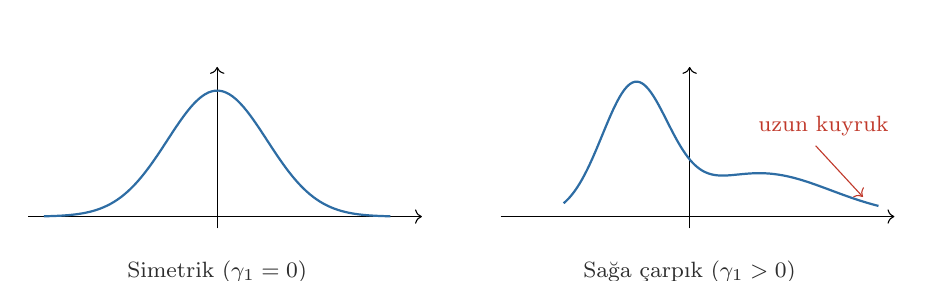
\begin{tikzpicture}[scale=1.0]
\begin{scope}
\draw[->] (-2.4,0)--(2.6,0); \draw[->] (0,-0.15)--(0,1.9);
\draw[grafikMavi,thick,domain=-2.2:2.2,samples=100] plot (\x,{1.6*exp(-\x*\x/0.8)});
\node[koyuGri] at (0,-0.7) {\footnotesize Simetrik ($\gamma_1=0$)};
\end{scope}
\begin{scope}[xshift=6cm]
\draw[->] (-2.4,0)--(2.6,0); \draw[->] (0,-0.15)--(0,1.9);
\draw[grafikMavi,thick,domain=-1.6:2.4,samples=120]
  plot (\x,{1.6*exp(-(\x+0.7)*(\x+0.7)/0.35)+0.55*exp(-(\x-0.9)*(\x-0.9)/1.6)});
\node[koyuGri] at (0,-0.7) {\footnotesize Sağa çarpık ($\gamma_1>0$)};
\draw[->,kirmizi] (1.6,0.9)--(2.2,0.25);
\node[kirmizi] at (1.7,1.15) {\footnotesize uzun kuyruk};
\end{scope}
\end{tikzpicture}
\end{center}
\vspace{0.45cm}

\begin{lstlisting}
for col in ['bill_length_mm','bill_depth_mm','flipper_length_mm','body_mass_g']:
    print(f"{col:>20}: skew={peng[col].skew():+.3f}  kurt={peng[col].kurt():+.3f}")
\end{lstlisting}

\begin{lstlisting}[style=outstyle]
      bill_length_mm: skew=+0.045  kurt=-0.883
       bill_depth_mm: skew=-0.150  kurt=-0.892
   flipper_length_mm: skew=+0.360  kurt=-0.961
         body_mass_g: skew=+0.472  kurt=-0.733
\end{lstlisting}

\bilgi{Dört değişkenin de \emph{fazla basıklığı} belirgin biçimde negatif
($\approx-0{,}9$). Bunun nedeni gerçek bir kalınlık farkı değil, verinin üç
farklı türün karışımı olması: iki tepeli (bimodal) bir dağılım basık görünür.
Bu, ham istatistiklere bakıp ``normal değil'' demeden önce \emph{gruplara}
bakmanın neden gerektiğinin güzel bir örneğidir.}

% =====================================================================
\gsec{Aykırı Değerler}
% =====================================================================

\nicin[Hangi Soruyu Cevaplıyor?]{Aykırı değer, ``diğerlerine hiç benzemeyen''
gözlemdir. Onları bulmak iki zıt sebeple önemlidir: bazen \textbf{gürültüdür}
(veri girişinde fazladan basılmış bir sıfır, bozuk sensör) ve analizini
zehirler; bazen de \textbf{aradığın şeyin ta kendisidir} (dolandırıcılık
işlemi, siber saldırı, arızalanmak üzere olan makine, nadir hastalık).

Bu yüzden aykırı değer tespiti hem bir \emph{veri temizleme} adımı, hem de
başlı başına bir \emph{makine öğrenmesi problemidir} (anomali tespiti,
Kısım 11).}

\begin{center}
\begin{tabularx}{\textwidth}{@{}>{\bfseries\color{anaMavi}}l >{$\displaystyle}l<{$} >{\raggedright\arraybackslash}X@{}}
\toprule
\rowcolor{acikMavi}\multicolumn{1}{@{}l}{\color{anaMavi}\textbf{Yöntem}} & \multicolumn{1}{l}{\color{anaMavi}\textbf{Ölçüt}} & \multicolumn{1}{l@{}}{\color{anaMavi}\textbf{Not}}\\
\midrule
IQR (Tukey) & x<Q_1-1{,}5\,\text{IQR}\ \text{ya da}\ x>Q_3+1{,}5\,\text{IQR} & Boxplot'un bıyıkları; dağılımdan bağımsız.\\
\rowcolor{acikGri} $z$-skoru & |z|>3 & Normallik varsayar; aykırı değerin kendisi $s$'yi şişirir.\\
Düzeltilmiş $z$ & 0{,}6745\,\dfrac{x-\tilde{x}}{\text{MAD}}>3{,}5 & Dayanıklı; küçük örneklemde tercih edilir.\\
\rowcolor{acikGri} Isolation Forest & \text{model tabanlı} & Çok değişkenli aykırılık (Kısım 10).\\
\bottomrule
\end{tabularx}
\end{center}

\begin{lstlisting}
q1, q3 = x.quantile(.25), x.quantile(.75)
iqr = q3 - q1
lo, hi = q1 - 1.5*iqr, q3 + 1.5*iqr
print(f"IQR sinirlari: [{lo:.0f}, {hi:.0f}]  aykiri sayisi = {((x<lo)|(x>hi)).sum()}")

z = np.abs(st.zscore(x))
print(f"|z| > 3           -> {(z > 3).sum()} gozlem")

mz = 0.6745*(x - x.median())/st.median_abs_deviation(x)
print(f"|duzeltilmis z| > 3.5 -> {(np.abs(mz) > 3.5).sum()} gozlem")
\end{lstlisting}

\begin{lstlisting}[style=outstyle]
IQR sinirlari: [1712, 6612]  aykiri sayisi = 0
|z| > 3           -> 0 gozlem
|duzeltilmis z| > 3.5 -> 0 gozlem
\end{lstlisting}

\nicin[Üç Ölçüt, Üç Farklı Felsefe]{\textbf{IQR (Tukey) kuralı --- niçin
1,5?} Bu sayı keyfi görünür ama değildir: veri normal dağılımlıysa
$Q_1-1{,}5\,\text{IQR}$ ile $Q_3+1{,}5\,\text{IQR}$ aralığı yaklaşık
$\mu\pm2{,}7\sigma$'ya karşılık gelir ve gözlemlerin \%99,3'ünü kapsar. Yani
Tukey, ``normal veride yüzde birden az yanlış alarm ver'' diye ayarlamıştır.
En büyük üstünlüğü: $Q_1$, $Q_3$ ve IQR aykırı değerlerden \emph{etkilenmez},
dolayısıyla ölçüt kendi kendini sabote etmez. Boxplot'un bıyıkları tam olarak
budur --- her boxplot'a baktığında aslında bu kuralı görüyorsun.

\textbf{$z$-skoru --- niçin tehlikeli?} $|z|>3$ ölçütü hem normallik varsayar
hem de bir kısır döngü içerir: aykırı değerin kendisi $\bar{x}$'i kaydırır ve
$s$'yi şişirir, bu da $z$'sini küçültür. Sonuç: \textbf{maskeleme}. $1, 2, 3,
4, 1000$ dizisinde 1000'in $z$-skoru yalnızca $1{,}79$'dur --- eşiği geçemez!
Küçük örneklemde $z$-skoru bir aykırı değeri asla 3'ün üstüne çıkaramaz;
matematiksel üst sınır $(n-1)/\sqrt{n}$'dir.

\textbf{Düzeltilmiş $z$ (MAD tabanlı) --- niçin en güvenlisi?} $\bar{x}$ yerine
medyanı, $s$ yerine MAD'ı kullanır; ikisi de aykırı değerlerden etkilenmez, bu
yüzden maskeleme olmaz. $0{,}6745$ katsayısı, normal dağılımda MAD'ı standart
sapmayla aynı ölçeğe getiren dönüşüm sabitidir --- böylece eşik yine
``$\sigma$ cinsinden'' okunabilir. Aynı $1,2,3,4,1000$ dizisinde düzeltilmiş
$z$ skoru 337 çıkar; yani problemi anında yakalar.

\textbf{Nerede hangisi?} Keşif ve görselleştirmede IQR (boxplot ile aynı dili
konuşur); büyük ve yaklaşık normal veride $z$; küçük, kirli veya kirliliğinden
şüphelendiğin veride MAD tabanlı düzeltilmiş $z$; birden çok değişkeni aynı
anda değerlendirmek gerektiğinde model tabanlı yöntemler (Isolation Forest,
Mahalanobis uzaklığı).}

\gercek[Ozon Deliğini 9 Yıl Geciktiren Aykırı Değer Filtresi]{1970'lerde
NASA'nın uydu verilerini işleyen yazılım, Antarktika üzerinde ölçülen çok
düşük ozon değerlerini ``fiziksel olarak imkânsız, demek ki sensör hatası''
diyerek otomatik olarak eliyordu. Ozon deliği 1985'te ancak yer istasyonundan
elle yapılan ölçümlerle keşfedildi; geri dönüp filtrelenen ham veriye
bakıldığında deliğin yıllardır orada olduğu görüldü.

Ders şu: \textbf{aykırı değeri otomatik silen her boru hattı, aynı zamanda
keşif yapma ihtimalini de siliyordur.} Doğru refleks silmek değil,
\emph{işaretlemek} ve incelemektir --- ve sildiğin her gözlemi raporunda
belirtmektir.}

\uyari{Aykırı değer bulmak, onu \emph{silmek} demek değildir. Üç soruyu sor:
(1) Ölçüm hatası mı? (2 metre boyunda bir penguen $\to$ sil.) (2) Farklı bir
popülasyondan mı geliyor? ($\to$ ayrı modelle.) (3) Gerçek ve önemli mi?
(Dolandırıcılık tespitinde \emph{aykırı değerler zaten aradığın şeydir}.)
Sessizce silmek, en ilginç bulguyu çöpe atmanın en hızlı yoludur.}

% =====================================================================
\gsec{İki Değişken Arasındaki İlişki: Korelasyon}
% =====================================================================

\nicin[Hangi Soruyu Cevaplıyor?]{Buraya kadar her değişkene tek tek baktık.
Ama gerçek sorular neredeyse hep \emph{ilişki} sorularıdır: Reklam harcaması
artınca satış artıyor mu? Uyku süresi sınav notunu etkiliyor mu? Hangi iki
sensör aslında aynı şeyi ölçüyor? Korelasyon, iki değişkenin
\textbf{birlikte hareket edip etmediğini} tek sayıya indirir.

Bu, tüm rehberin geri kalanının kapısıdır: regresyon ``bu ilişkiyi bir
denklemle yaz'' der, öznitelik seçimi ``hangi değişken hedefle ilişkili?''
diye sorar, PCA ``birbiriyle ilişkili değişkenleri birleştir'' der. Hepsinin
altında korelasyon vardır.}

\form[Pearson Korelasyonu]{
\[
r=\frac{\sum(x_i-\bar{x})(y_i-\bar{y})}{\sqrt{\sum(x_i-\bar{x})^2}\sqrt{\sum(y_i-\bar{y})^2}}
=\frac{\Cov(x,y)}{s_xs_y}\in[-1,1]
\]
\textbf{Doğrusal} ilişkinin gücünü ölçer. $r^2$, bir değişkenin diğerindeki
değişkenliğin ne kadarını açıkladığını verir.}

\nicin{\textbf{Formülü parçalayalım.} Pay $\sum(x_i-\bar{x})(y_i-\bar{y})$
\emph{kovaryanstır} ve bütün fikri o taşır: her gözlem için ``$x$ kendi
ortalamasının hangi tarafında?'' ve ``$y$ kendi ortalamasının hangi
tarafında?'' diye sorar, ikisini çarpar. Her ikisi de üstteyse çarpım pozitif,
her ikisi de alttaysa (eksi $\times$ eksi) yine pozitif; biri üstte biri
alttaysa negatif. Toplam pozitifse ``birlikte artıyorlar'', negatifse ``biri
artarken diğeri azalıyor'' demektir.

\textbf{Payda niçin var?} Çünkü kovaryansın tek başına bir sorunu vardır:
birimi $x$'in birimi çarpı $y$'nin birimidir ve ölçeğe bağlıdır. Boy--kilo
kovaryansı, boyu santimetre yerine milimetre ölçersen 10 katına çıkar --- oysa
ilişki değişmedi. İki standart sapmaya bölmek bu keyfîliği yok eder ve sonucu
$[-1,+1]$ aralığına hapseder. Yani \textbf{$r$, ``birimsizleştirilmiş
kovaryanstır''} ve bu sayede boy--kilo ilişkisiyle sıcaklık--satış ilişkisi
aynı cetvelle karşılaştırılabilir.

\textbf{$r^2$'yi nasıl okumalı?} $r=0{,}873$ (yüzgeç uzunluğu -- ağırlık) ise
$r^2=0{,}76$: ağırlıktaki değişkenliğin \%76'sı yüzgeç uzunluğuyla
``açıklanıyor'', \%24'ü başka şeylerden geliyor. Bu, regresyondaki $R^2$'nin
ta kendisidir.

\textbf{Nerede kullanılır?}
\begin{itemize}\itemsep1pt
\item \textbf{Öznitelik seçimi:} Hedefle korelasyonu sıfıra yakın öznitelikler
ilk elemede düşer; birbiriyle $|r|>0{,}9$ olan iki öznitelikten biri atılır
(çoklu doğrusal bağlantı, Kısım 7).
\item \textbf{Portföy yönetimi:} Riski düşürmenin yolu getirileri birbiriyle
\emph{düşük korelasyonlu} varlıkları bir arada tutmaktır. Çeşitlendirmenin
tüm matematiği korelasyon matrisidir.
\item \textbf{Ölçüm doğrulama:} Yeni ve ucuz bir sensörün, pahalı referans
cihazla korelasyonu ölçülerek güvenilirliği sınanır.
\item \textbf{Öneri sistemleri:} ``Senin gibi kullanıcılar'' derken kastedilen,
puanlama vektörleri yüksek korelasyonlu kullanıcılardır.
\end{itemize}}

\uyari{$r=0$ ``ilişki yok'' demek \emph{değildir}; ``\textbf{doğrusal} ilişki
yok'' demektir. $y=x^2$ verisinde $-3\dots3$ aralığında $r\approx0$ çıkar,
oysa $y$ tamamen $x$ tarafından belirlenir. Bu yüzden korelasyona bakmadan
önce daima saçılım grafiği çizilir --- bir sonraki iki bölüm tam olarak bunun
niçin hayati olduğunu gösteriyor.}

\begin{center}
\begin{tabularx}{\textwidth}{@{}>{\bfseries\color{anaMavi}}l >{\raggedright\arraybackslash}X >{\raggedright\arraybackslash}X@{}}
\toprule
\rowcolor{acikMavi}\multicolumn{1}{@{}l}{\color{anaMavi}\textbf{Katsayı}} & \multicolumn{1}{l}{\color{anaMavi}\textbf{Ölçtüğü}} & \multicolumn{1}{l@{}}{\color{anaMavi}\textbf{Ne zaman?}}\\
\midrule
Pearson $r$ & Doğrusal ilişki & Sürekli, yaklaşık normal, aykırı değer yok.\\
\rowcolor{acikGri} Spearman $\rho$ & Monoton ilişki (sıralara Pearson) & Sıralayıcı veri, doğrusal olmayan monoton ilişki, aykırı değer var.\\
Kendall $\tau$ & Uyumlu/uyumsuz çift oranı & Küçük örneklem, çok sayıda eşit değer (tie).\\
\bottomrule
\end{tabularx}
\end{center}

\begin{lstlisting}
num = peng.select_dtypes('number')
print(num.corr().round(3))
\end{lstlisting}

\begin{lstlisting}[style=outstyle]
                   bill_length_mm  bill_depth_mm  flipper_length_mm  body_mass_g
bill_length_mm              1.000         -0.229              0.653        0.589
bill_depth_mm              -0.229          1.000             -0.578       -0.472
flipper_length_mm           0.653         -0.578              1.000        0.873
body_mass_g                 0.589         -0.472              0.873        1.000
\end{lstlisting}

\begin{lstlisting}
from scipy import stats as st
a, b = peng.bill_length_mm, peng.body_mass_g
print(f"Pearson  = {st.pearsonr(a, b).statistic:.3f}")
print(f"Spearman = {st.spearmanr(a, b).statistic:.3f}")
print(f"Kendall  = {st.kendalltau(a, b).statistic:.3f}")
# Pearson  = 0.589 / Spearman = 0.576 / Kendall = 0.428
\end{lstlisting}

\gsub{Simpson Paradoksu: Gerçek Bir Örnek}

Korelasyon matrisinde gaga uzunluğu ile gaga derinliği arasında
\textbf{negatif} bir ilişki ($r=-0{,}229$) görünüyor: uzun gagalı penguenlerin
gagası daha ince. Şimdi aynı hesabı \emph{tür içinde} yapalım.

\begin{lstlisting}
r_all = st.pearsonr(peng.bill_length_mm, peng.bill_depth_mm)
print(f"TUM veri:  r = {r_all.statistic:+.3f}  (p = {r_all.pvalue:.2e})")

for sp, g in peng.groupby('species'):
    r = st.pearsonr(g.bill_length_mm, g.bill_depth_mm)
    print(f"{sp:>10}: r = {r.statistic:+.3f}  (p = {r.pvalue:.4f}, n={len(g)})")
\end{lstlisting}

\begin{lstlisting}[style=outstyle]
TUM veri:  r = -0.229  (p = 2.53e-05)
    Adelie: r = +0.386  (p = 0.0000, n=146)
 Chinstrap: r = +0.654  (p = 0.0000, n=68)
    Gentoo: r = +0.654  (p = 0.0000, n=119)
\end{lstlisting}

\uyari{\textbf{Simpson paradoksu}: ilişkinin işareti gruplar birleştirilince
tersine döner. Burada gerçek şu: her tür içinde uzun gaga = derin gaga
(pozitif). Ama Gentoo'lar hem uzun hem \emph{ince} gagalıdır ve veri setinin
üçte birini oluşturur; türleri karıştırınca bu üçüncü değişken (tür)
ilişkinin işaretini çevirir. \textbf{Ders:} bir korelasyonu raporlamadan önce
``hangi gizli grup değişkeni bunu açıklıyor olabilir?'' diye sor.}

\begin{lstlisting}
import matplotlib.pyplot as plt, seaborn as sns

fig, (a1, a2) = plt.subplots(1, 2, figsize=(11, 4.5), sharey=True)
sns.regplot(data=peng, x='bill_length_mm', y='bill_depth_mm',
            ax=a1, scatter_kws={'s': 18, 'alpha': .6}, line_kws={'color': 'C3'})
a1.set_title('Tum veri: r = -0.23  (yaniltici)')
sns.scatterplot(data=peng, x='bill_length_mm', y='bill_depth_mm',
                hue='species', ax=a2, s=22)
for sp, g in peng.groupby('species'):
    sns.regplot(data=g, x='bill_length_mm', y='bill_depth_mm',
                ax=a2, scatter=False, ci=None)
a2.set_title('Tur bazinda: r > 0  (dogru)')
plt.tight_layout(); plt.show()
\end{lstlisting}

\ipucu{\textbf{Korelasyon nedensellik değildir} --- ama nedensellik neredeyse
her zaman korelasyon üretir. Bir $r$ değeri gördüğünde üç alternatif açıklama
her zaman masadadır: (1) $X\to Y$, (2) $Y\to X$, (3) gizli bir $Z$ ikisini de
etkiliyor (\emph{confounding}). Üçüncüsünü elemenin tek kesin yolu
\textbf{randomize deneydir}; gözlemsel veride ancak kontrol değişkenleriyle
yaklaşabilirsin.}

\gsub{Anscombe Dörtlüsü: Neden Grafik Çizmelisin?}

\begin{lstlisting}
ans = sns.load_dataset('anscombe')
ozet = ans.groupby('dataset').apply(
    lambda g: pd.Series({
        'x_mean': g.x.mean(), 'y_mean': g.y.mean(),
        'x_std': g.x.std(),  'y_std': g.y.std(),
        'r': st.pearsonr(g.x, g.y).statistic}),
    include_groups=False).round(2)
print(ozet)
\end{lstlisting}

\begin{lstlisting}[style=outstyle]
         x_mean  y_mean  x_std  y_std     r
dataset                                    
I           9.0     7.5   3.32   2.03  0.82
II          9.0     7.5   3.32   2.03  0.82
III         9.0     7.5   3.32   2.03  0.82
IV          9.0     7.5   3.32   2.03  0.82
\end{lstlisting}

\uyari{Dört veri setinin ortalaması, standart sapması ve korelasyonu
\emph{aynı} --- ama grafikleri tamamen farklıdır: biri doğrusal, biri parabol,
biri tek aykırı değerin sürüklediği bir doğru, biri de tek bir noktanın
yarattığı sahte ilişki. \textbf{Özet istatistik asla grafiğin yerini tutmaz.}}

% #####################################################################
\gpart{3}{Olasılık Teorisi}
% #####################################################################

% =====================================================================
\gsec{Temel Kavramlar ve Aksiyomlar}
% =====================================================================

\tanim{Bir \emph{rastgele deneyin} tüm olası sonuçlarının kümesine
\textbf{örnek uzay} ($\Omega$), örnek uzayın alt kümelerine \textbf{olay}
denir. Olasılık, olaylara $[0,1]$ aralığında sayı atayan bir fonksiyondur.}

\form[Kolmogorov Aksiyomları]{
\begin{enumerate}\itemsep1pt
\item $\Prob(A)\ge0$ (negatif olmama),
\item $\Prob(\Omega)=1$ (normalizasyon),
\item Ayrık $A_1,A_2,\dots$ için
$\Prob\!\left(\bigcup_i A_i\right)=\sum_i\Prob(A_i)$ (toplanabilirlik).
\end{enumerate}
Bütün olasılık kuralları bu üçünden türetilir.}

\nicin{\textbf{Aksiyom ne demek, niçin gerekli?} Aksiyom, ispatlanmayan ama
kabul edilen başlangıç kuralıdır. Kolmogorov 1933'te şunu fark etti:
olasılığı ``uzun vadede görülme sıklığı'' ya da ``inanç derecesi'' diye
tanımlamaya çalışmak felsefi tartışma doğuruyor, oysa \emph{nasıl
davranması gerektiğini} üç kuralla sabitlersen bütün matematik kendiliğinden
gelir. Bu üç madde, olasılığın ``oyun kurallarıdır''.

\textbf{Her biri sezgisel olarak ne diyor?}
\begin{itemize}\itemsep1pt
\item[(1)] \emph{Negatif olamaz.} ``Yarın yağmur yağma olasılığı $-0{,}3$''
cümlesinin bir anlamı yok.
\item[(2)] \emph{Bir şeyin olma olasılığı 1'dir.} Tüm sonuçları listeledinse,
bunlardan birinin gerçekleşeceği kesindir. Bütün yüzdelerin toplamı \%100
etmelidir.
\item[(3)] \emph{Ayrık olayların olasılıkları toplanır.} Zar 1 veya 2
gelme olasılığı $1/6+1/6$'dır --- çünkü ikisi aynı anda olamaz. Aynı anda
olabilseydi çakışmayı iki kez sayardık; toplama kuralındaki
$-\Prob(A\cap B)$ terimi tam olarak bu düzeltmedir.
\end{itemize}

\textbf{Bu soyutluk nerede işe yarıyor?} Aksiyomlar sayesinde
\emph{olasılık} kelimesi çok farklı şeyleri aynı matematikle modelleyebilir:
bir zarın yüzü, bir e-postanın spam olması, bir hastanın iyileşmesi, bir
sinir ağının çıktı katmanındaki \code{softmax} değerleri. \code{softmax}'ın
niçin üstel alıp toplama böldüğünü merak ettiysen cevabı budur: negatif
olmama (üstel) ve toplamın 1 olması (normalizasyon) aksiyomlarını zorla
sağlatıyor. Bir modelin çıktısına ``olasılık'' diyebilmenin bedeli bu üç
kuralı sağlamaktır.}

\begin{center}
\begin{tabularx}{\textwidth}{@{}>{\bfseries\color{anaMavi}}l >{$\displaystyle}l<{$} >{\raggedright\arraybackslash}X@{}}
\toprule
\rowcolor{acikMavi}\multicolumn{1}{@{}l}{\color{anaMavi}\textbf{Kural}} & \multicolumn{1}{l}{\color{anaMavi}\textbf{Formül}} & \multicolumn{1}{l@{}}{\color{anaMavi}\textbf{Not}}\\
\midrule
Tümleyen & \Prob(A^c)=1-\Prob(A) & ``En az bir'' problemlerinde vazgeçilmez.\\
\rowcolor{acikGri} Toplama & \Prob(A\cup B)=\Prob(A)+\Prob(B)-\Prob(A\cap B) & Kesişim iki kez sayılmasın.\\
Koşullu & \Prob(A\mid B)=\dfrac{\Prob(A\cap B)}{\Prob(B)} & $\Prob(B)>0$ olmalı.\\
\rowcolor{acikGri} Çarpma & \Prob(A\cap B)=\Prob(A\mid B)\Prob(B) & Zincirleme genişletilebilir.\\
Bağımsızlık & \Prob(A\cap B)=\Prob(A)\Prob(B) & Eşdeğeri: $\Prob(A\mid B)=\Prob(A)$.\\
\rowcolor{acikGri} Toplam olasılık & \Prob(A)=\sum_i\Prob(A\mid B_i)\Prob(B_i) & $\{B_i\}$ örnek uzayı böler.\\
\bottomrule
\end{tabularx}
\end{center}

\uyari{\textbf{Bağımsızlık} ile \textbf{ayrıklık} (mutually exclusive)
karıştırılır ama zıt kavramlardır. Ayrık olaylar ($A\cap B=\emptyset$)
olabildiğince \emph{bağımlıdır}: biri olduysa diğeri kesinlikle olmamıştır.
Olasılığı pozitif iki olay hem ayrık hem bağımsız olamaz.}

% =====================================================================
\gsec{Koşullu Olasılık: Titanic Üzerinde}
% =====================================================================

Koşullu olasılık, ``elimizdeki bilgiyi kullanarak olasılığı güncellemek''
demektir. 891 Titanic yolcusuyla somutlaştıralım.

\nicin[Niçin En Önemli Kavram?]{$\Prob(A\mid B)=\Prob(A\cap B)/\Prob(B)$
formülü basit görünür, ama yaptığı şey derindir: \textbf{örnek uzayı
daraltır}. Payda artık $\Omega$ değil $B$'dir --- yani ``$B$ olduğunu
öğrendim, dünyam küçüldü, şimdi bu küçük dünyada $A$ ne kadar yer
kaplıyor?'' diye soruyorsun. Titanic'te ``bir yolcunun hayatta kalma
olasılığı \%38'' cümlesi, ``kadın olduğunu biliyorsam \%74'' cümlesine
dönüşür. Aynı olay, farklı bilgi, farklı olasılık.

\textbf{Niçin bu kadar merkezî?} Çünkü \emph{tahmin} kelimesinin kendisi
koşullu olasılıktır. Bir makine öğrenmesi modeli ne yapar?
$\Prob(\text{sınıf}\mid \text{öznitelikler})$ hesaplar. Lojistik regresyon,
Naive Bayes, rastgele orman, sinir ağı --- hepsi bu tek ifadeyi farklı
yollardan kestirmeye çalışır. Koşullu olasılığı anlamak, bütün denetimli
öğrenmenin ne yaptığını anlamaktır.

\textbf{Nerede karşına çıkar?} Tıbbi teşhis (semptom verildiğinde hastalık),
spam filtresi (kelimeler verildiğinde spam), kredi skoru (geçmiş verildiğinde
temerrüt), öneri sistemi (izlenenler verildiğinde beğeni), dil modelleri
(önceki kelimeler verildiğinde sonraki kelime). Sonuncusu dikkat çekicidir:
büyük dil modelleri devasa bir $\Prob(\text{sonraki jeton}\mid
\text{bağlam})$ hesaplayıcısıdır.}

\begin{lstlisting}
import pandas as pd, seaborn as sns
tit = sns.load_dataset('titanic')

tab = pd.crosstab(tit['sex'], tit['survived'])
print(tab)
print("\nSatir yuzdeleri:")
print((tab.div(tab.sum(axis=1), axis=0)*100).round(1))
\end{lstlisting}

\begin{lstlisting}[style=outstyle]
survived    0    1
sex               
female     81  233
male      468  109

Satir yuzdeleri:
survived     0     1
sex                 
female    25.8  74.2
male      81.1  18.9
\end{lstlisting}

\begin{lstlisting}
print("P(survived)          =", round(tit.survived.mean(), 4))
print("P(survived | female) =", round(tit.loc[tit.sex=='female','survived'].mean(), 4))
print("P(survived | male)   =", round(tit.loc[tit.sex=='male',  'survived'].mean(), 4))
print("P(female | survived) =", round((tit.loc[tit.survived==1,'sex']=='female').mean(), 4))
\end{lstlisting}

\begin{lstlisting}[style=outstyle]
P(survived)          = 0.3838
P(survived | female) = 0.742
P(survived | male)   = 0.1889
P(female | survived) = 0.6813
\end{lstlisting}

\uyari{$\Prob(A\mid B)$ ile $\Prob(B\mid A)$ \textbf{aynı şey değildir} ve bu,
istatistikteki en yaygın akıl yürütme hatasıdır (\emph{koşulun ters
çevrilmesi}). Burada $\Prob(\text{hayatta}\mid\text{kadın})=0{,}742$ iken
$\Prob(\text{kadın}\mid\text{hayatta})=0{,}681$. İkisi ancak marjinal
olasılıklar eşitse çakışır.}

\gsub{Bayes Teoremi}

\form[Bayes]{
\[
\Prob(A\mid B)=\frac{\Prob(B\mid A)\,\Prob(A)}{\Prob(B)}
=\frac{\Prob(B\mid A)\Prob(A)}{\sum_i\Prob(B\mid A_i)\Prob(A_i)}
\]
Sözle: \emph{sonsal} $\propto$ \emph{olabilirlik} $\times$ \emph{önsel}.}

\nicin{\textbf{Bayes ne yapıyor?} Koşulu \emph{ters çevirir}. Elinde
$\Prob(B\mid A)$ var ama sana lazım olan $\Prob(A\mid B)$. Bu ikisi
\emph{aynı şey değildir} ve karıştırmak istatistikteki en pahalı hatadır:
``hasta olan birinin testi pozitif çıkma olasılığı'' ile ``testi pozitif
çıkan birinin hasta olma olasılığı'' tamamen farklı sayılardır.

\textbf{Dört terimin adı ve anlamı:}
\begin{itemize}\itemsep1pt
\item $\Prob(A)$ --- \textbf{önsel} (prior): Kanıtı görmeden önceki inancın.
``Bu hastalık toplumda binde bir görülür.''
\item $\Prob(B\mid A)$ --- \textbf{olabilirlik} (likelihood): Hipotez doğruysa
bu kanıtı görme şansın. ``Hastaysa test \%99 pozitif verir.''
\item $\Prob(B)$ --- \textbf{kanıt} (evidence): Kanıtın her ihtimal altında
toplam görülme olasılığı. Yalnızca normalizasyon içindir; sonucun 0--1
aralığında kalmasını sağlar.
\item $\Prob(A\mid B)$ --- \textbf{sonsal} (posterior): Kanıtı gördükten
sonraki güncellenmiş inancın. Aradığın sayı budur.
\end{itemize}

\textbf{Niçin bu kadar güçlü?} Çünkü \emph{öğrenmenin} matematiksel tarifidir:
bir inancın vardı, veri geldi, inancını güncelledin. Yeni veri gelince
bugünün sonsalı yarının önseli olur. Bu döngü, bir hekimin teşhis sürecinden
bir Kalman filtresinin uydu konumu düzeltmesine kadar aynıdır.

\textbf{En kritik ders --- önsel her şeyi değiştirir.} Aynı test sonucu,
hastalığın yaygınlığına göre ``\%2 ihtimalle hastasın'' ya da ``\%83 ihtimalle
hastasın'' anlamına gelebilir. Bir sonraki sayfadaki tablo tam olarak bunu
gösteriyor. Kanıtı önselden koparıp yorumlamak, sayının kendisini
anlamsızlaştırır.}

\gercek[Bayes'in Günlük Hayattaki Dört Yüzü]{
\begin{itemize}\itemsep1pt
\item \textbf{Spam filtresi:} ``Ücretsiz'' kelimesi geçen bir e-posta geldi.
Filtre $\Prob(\text{spam}\mid\text{``ücretsiz''})$ hesaplar. Önsel: gelen
postaların \%40'ı spam. Olabilirlik: spam'lerin \%15'inde, normal postaların
\%1'inde bu kelime geçer. Sonsal $\approx\%91$. Naive Bayes sınıflandırıcısı
(Kısım 9) tam olarak budur --- yüzlerce kelime için bunu yapıp çarpar.
\item \textbf{Adli tıp:} DNA eşleşme olasılığı milyonda birdir. Savcı
``o hâlde sanığın masum olma ihtimali milyonda bir'' der --- bu
\textbf{savcı yanılgısıdır}. 10 milyon kişilik bir şehirde tesadüfen eşleşen
$\approx10$ kişi vardır; başka kanıt yoksa sanığın suçlu olma olasılığı
\%10'dur, \%99,9999 değil. Bu hata gerçek mahkemelerde masum insanları
hapse attı.
\item \textbf{Arama kurtarma:} Kayıp bir denizaltı ya da uçak aranırken
deniz haritası hücrelere bölünür, her hücreye bir önsel olasılık verilir.
Bir hücre aranıp bulunamazsa \emph{tüm haritanın} olasılıkları Bayes ile
güncellenir. Air France 447 enkazı 2011'de tam bu yöntemle bulundu.
\item \textbf{A/B testi:} ``B versiyonu A'dan iyidir'' inancını, gelen her
yeni ziyaretçiyle güncellersin. Kısım 6'daki Bayesçi çıkarım bölümü bunun
uygulamasıdır --- ve bir pazarlama müdürüne ``$p<0{,}05$'' demektense
``\%94 ihtimalle B daha iyi'' demek çok daha kullanışlıdır.
\end{itemize}}

\begin{lstlisting}
pf  = (tit.sex == 'female').mean()                              # onsel P(female)
psf = tit.loc[tit.sex == 'female', 'survived'].mean()            # P(surv | female)
ps  = tit.survived.mean()                                        # kanit P(surv)
print("Bayes ile P(female | survived) =", round(psf*pf/ps, 4))   # 0.6813
\end{lstlisting}

\gsub{Klasik Tuzak: Tıbbi Tarama Testi}

\soru{Bir hastalık toplumda \%0,1 oranında görülüyor. Test, hastaları \%99
doğrulukla yakalıyor (\emph{duyarlılık}) ve sağlıklıları \%95 doğrulukla
eliyor (\emph{özgüllük}). Testin \emph{pozitif} çıktı. Gerçekten hasta olma
olasılığın nedir?}

\cozum Sezgi ``\%99'' der; doğru cevap \%2'dir.
\[
\Prob(H\mid+)=\frac{0{,}99\times0{,}001}{0{,}99\times0{,}001+0{,}05\times0{,}999}
=\frac{0{,}00099}{0{,}05094}=0{,}0194 .
\]

\begin{lstlisting}
sens, spec = 0.99, 0.95
for prev in [0.001, 0.01, 0.05, 0.2]:
    p_pos = sens*prev + (1 - spec)*(1 - prev)
    ppv = sens*prev/p_pos
    print(f"yayginlik = {prev:6.3f}  ->  P(hasta | +) = {ppv:.4f}")
\end{lstlisting}

\begin{lstlisting}[style=outstyle]
yayginlik =  0.001  ->  P(hasta | +) = 0.0194
yayginlik =  0.010  ->  P(hasta | +) = 0.1667
yayginlik =  0.050  ->  P(hasta | +) = 0.5103
yayginlik =  0.200  ->  P(hasta | +) = 0.8319
\end{lstlisting}

\bilgi{\textbf{Taban oranı yanılgısı} (base rate fallacy): nadir bir olayda,
mükemmele yakın bir test bile çok sayıda \emph{yalancı pozitif} üretir. Bu,
makine öğrenmesinde dengesiz veri probleminin (Kısım 11) tam karşılığıdır:
\%99,9 doğruluk, taban oranı \%0,1 olan bir problemde hiçbir şey ifade etmez.
Aynı hesap, sınıflandırma metriklerinde \emph{kesinlik} (precision) adıyla
karşımıza çıkacak.}

\gsub{Kontenjans Tablosunda Bağımsızlık}

\begin{lstlisting}
from scipy import stats as st
chi2, p, dof, exp = st.chi2_contingency(tab)
print(f"chi2 = {chi2:.2f}   dof = {dof}   p = {p:.3e}")
print("Bagimsizlik altinda BEKLENEN sayilar:")
print(pd.DataFrame(exp, index=tab.index, columns=tab.columns).round(1))
\end{lstlisting}

\begin{lstlisting}[style=outstyle]
chi2 = 260.72   dof = 1   p = 1.197e-58
Bagimsizlik altinda BEKLENEN sayilar:
survived      0      1
sex                   
female    193.5  120.5
male      355.5  221.5
\end{lstlisting}

Gözlenen 233 kadın hayatta kalanına karşılık bağımsızlık altında beklenen
sayı yalnızca 120,5. Cinsiyet ile hayatta kalma \emph{kesinlikle} bağımsız
değil.

\gsub{Koşullamaya Devam: Üçüncü Değişken}

\begin{lstlisting}
print(tit.groupby(['pclass','sex'])['survived'].agg(['count','mean']).round(3))
\end{lstlisting}

\begin{lstlisting}[style=outstyle]
               count   mean
pclass sex                 
1      female     94  0.968
       male      122  0.369
2      female     76  0.921
       male      108  0.157
3      female    144  0.500
       male      347  0.135
\end{lstlisting}

\ornek{1.\ sınıf kadın yolcuların \%96,8'i, 3.\ sınıf erkeklerin ise yalnızca
\%13,5'i hayatta kalmış. ``Kadınlar ve çocuklar önce'' kuralı sınıf farkıyla
birleşince 7 kata varan bir fark üretiyor. Bu tablo, Kısım 7'de kuracağımız
lojistik regresyonun neden \code{sex} ve \code{pclass} değişkenlerini birlikte
kullanması gerektiğini gösteriyor.}

% =====================================================================
\gsec{Kombinatorik ve Simülasyon}
% =====================================================================

\nicin[Sayma Niçin Olasılığın Temeli?]{Tüm sonuçlar eşit olasılıklıysa
olasılık sadece bir bölme işlemidir:
$\Prob(A) = \frac{\text{istenen sonuç sayısı}}{\text{tüm sonuç sayısı}}$.
Sorun şu ki bu iki sayı çoğunlukla elle sayılamayacak kadar büyüktür ---
52 kartlık desteden 5 kart seçmenin 2.598.960 yolu vardır. Kombinatorik,
\textbf{listelemeden sayma sanatıdır}.

\textbf{Dört formülü ayıran iki soru:} (1) \emph{Sıra önemli mi?}
Şifre için evet (``ab'' $\ne$ ``ba''), loto kuponu için hayır. (2)
\emph{İade var mı?} Zar atmada evet (aynı sayı tekrar gelebilir), kart
çekmede hayır. Bu iki sorunun cevabı hangi formülü kullanacağını doğrudan
belirler --- ezberlemek yerine her seferinde bu iki soruyu sor.

\textbf{Kombinasyon formülü niçin öyle?} $\binom{n}{r}=\frac{n!}{r!(n-r)!}$
şöyle okunur: önce sıralı seç ($n!/(n-r)!$), sonra aynı $r$ elemanın
$r!$ farklı sıralanışını tek saymak için $r!$'e böl. Yani kombinasyon,
``permütasyonun fazla saydığını düzeltmesidir''.

\textbf{Nerede kullanılır?}
\begin{itemize}\itemsep1pt
\item \textbf{Şifre güvenliği:} 8 karakterli, 62 sembollü bir şifrenin
$62^8\approx2{,}2\times10^{14}$ ihtimali vardır. Modern bir GPU saniyede
$10^{10}$ deneme yapar --- yani 6 saat. Şifreyi 12 karaktere çıkarınca süre
34.000 yıla fırlar. Güvenlik politikalarının arkasındaki tek matematik budur.
\item \textbf{A/B/n test tasarımı:} 4 başlık $\times$ 3 görsel $\times$ 2 buton
rengi $=24$ varyant. Çarpım kuralı, ``kaç kullanıcıya ihtiyacım var?''
sorusunun ilk adımıdır.
\item \textbf{Makine öğrenmesi:} $k$ katlı çapraz doğrulamada kaç farklı
eğitim kümesi oluşur; \code{GridSearchCV}'de parametre ızgarasının boyutu
(3 parametrenin her biri 5 değer $\to$ 125 model); rastgele ormanın her
düğümde $\binom{p}{m}$ öznitelik alt kümesinden seçim yapması.
\item \textbf{Karma çakışması:} Doğum günü problemi, 128 bitlik bir karma
fonksiyonunun niçin $2^{64}$ kayıttan sonra çakışmaya başladığını söyler ---
kriptografideki ``doğum günü sınırı''.
\end{itemize}}

\begin{center}
\begin{tabularx}{\textwidth}{@{}>{\bfseries\color{anaMavi}}l >{$\displaystyle}l<{$} >{\raggedright\arraybackslash}X@{}}
\toprule
\rowcolor{acikMavi}\multicolumn{1}{@{}l}{\color{anaMavi}\textbf{Sayma}} & \multicolumn{1}{l}{\color{anaMavi}\textbf{Formül}} & \multicolumn{1}{l@{}}{\color{anaMavi}\textbf{Ne zaman?}}\\
\midrule
Çarpım kuralı & n_1n_2\cdots n_k & Bağımsız aşamalar.\\
\rowcolor{acikGri} Permütasyon & P(n,r)=\dfrac{n!}{(n-r)!} & Sıra önemli, iadesiz.\\
Kombinasyon & \binom{n}{r}=\dfrac{n!}{r!(n-r)!} & Sıra önemsiz, iadesiz.\\
\rowcolor{acikGri} Tekrarlı & n^r & Sıra önemli, iadeli.\\
\bottomrule
\end{tabularx}
\end{center}

\begin{lstlisting}
from math import comb, perm, factorial
from itertools import combinations, permutations

print(comb(49, 6))        # 13983816  -> 6/49 loto: tek kombinasyon olasiligi 1/13.98M
print(perm(10, 3))        # 720
print(factorial(5))       # 120

# Poker: full house olasiligi
toplam = comb(52, 5)
full_house = 13*comb(4,3)*12*comb(4,2)
print(f"P(full house) = {full_house/toplam:.6f}")     # 0.001441
\end{lstlisting}

\gsub{Doğum Günü Problemi}

\soru{Bir sınıfta kaç kişi olursa en az ikisinin doğum günü aynı olma
olasılığı \%50'yi geçer?}

\cozum Tümleyenle çalışmak çok daha kolaydır:
\[
\Prob(\text{en az bir ortak})=1-\frac{365}{365}\cdot\frac{364}{365}\cdots\frac{365-n+1}{365}.
\]

\begin{lstlisting}
def p_ortak_dogumgunu(n):
    p = 1.0
    for i in range(n):
        p *= (365 - i)/365
    return 1 - p

for n in [10, 23, 30, 50, 70]:
    print(f"n = {n:>3}: P = {p_ortak_dogumgunu(n):.4f}")
\end{lstlisting}

\begin{lstlisting}[style=outstyle]
n =  10: P = 0.1169
n =  23: P = 0.5073
n =  30: P = 0.7063
n =  50: P = 0.9704
n =  70: P = 0.9992
\end{lstlisting}

\bilgi{23 kişi yeter. Sezgiye aykırı gelmesinin nedeni, ``benimle aynı'' değil
``herhangi iki kişi aynı'' sorusunun sorulmasıdır: 23 kişide
$\binom{23}{2}=253$ çift vardır. Aynı mantık, karma (hash) çakışmalarında ve
kriptografideki \emph{doğum günü saldırısında} karşımıza çıkar.}

\gsub{Monty Hall: Simülasyonla İnanmak}

\begin{lstlisting}
import numpy as np
rng = np.random.default_rng(42)
n = 200_000

odul  = rng.integers(0, 3, n)      # odulun oldugu kapi
secim = rng.integers(0, 3, n)      # yarismacinin ilk secimi

# Sunucu bos bir kapi acar; DEGISTIRMEK, ilk secim yanlissa kazandirir
print(f"kalma      -> kazanma orani = {(secim == odul).mean():.4f}")
print(f"degistirme -> kazanma orani = {(secim != odul).mean():.4f}")
\end{lstlisting}

\begin{lstlisting}[style=outstyle]
kalma      -> kazanma orani = 0.3353
degistirme -> kazanma orani = 0.6647
\end{lstlisting}

\ipucu{Bir olasılık sonucundan emin olamadığında \textbf{simüle et}. Beş
satırlık bir Monte Carlo, saatlerce süren tartışmayı bitirir. Aynı teknik
Kısım 5'te bootstrap, Kısım 6'da permütasyon testi olarak karşımıza
çıkacak --- hepsi aynı fikrin farklı kılıklarıdır.}

% =====================================================================
\gsec{Rastgele Değişkenler}
% =====================================================================

\tanim{\textbf{Rastgele değişken} $X$, örnek uzaydaki her sonuca bir sayı
atayan fonksiyondur. \emph{Kesikli} ise olasılık kütle fonksiyonu (PMF)
$p(x)=\Prob(X=x)$, \emph{sürekli} ise olasılık yoğunluk fonksiyonu (PDF)
$f(x)$ ile tanımlanır. Her ikisinde de birikimli dağılım fonksiyonu
$F(x)=\Prob(X\le x)$'tir.}

\nicin{\textbf{Niçin böyle bir fonksiyona ihtiyaç var?} Çünkü olasılık teorisi
``yazı/tura'', ``kırmızı/mavi'' gibi \emph{etiketlerle} değil, sayılarla
çalışmak ister --- ancak o zaman toplama, ortalama alma, integral gibi
araçları kullanabilirsin. Rastgele değişken, gerçek dünyadaki sonuçları
sayı doğrusuna taşıyan çevirmen katmanıdır: ``tura'' $\to 1$, ``yazı'' $\to
0$; ``müşteri geldi'' $\to$ harcadığı tutar; ``sunucu yanıtladı'' $\to$
milisaniye.

\textbf{Kesikli mi sürekli mi --- niçin önemli?} Bu ayrım hangi araçları
kullanacağını belirler: kesikli olanda \emph{toplam}, sürekli olanda
\emph{integral}; kesikli olanda $\Prob(X=3)$ anlamlıdır, sürekli olanda
sıfırdır. Pratikte: sayılabilen şeyler (günlük sipariş adedi, hatalı ürün
sayısı, tıklama var/yok) kesikli; ölçülen şeyler (ağırlık, süre, sıcaklık,
gelir) süreklidir.

\textbf{CDF niçin PMF/PDF'ten daha kullanışlı?} Çünkü $F(x)=\Prob(X\le x)$
her ikisi için de aynı biçimde tanımlıdır ve doğrudan cevap verdiği sorular
gerçek hayatta sorulan sorulardır: ``Teslimatın 3 günden erken gelme
olasılığı?'' ($F(3)$), ``Yüklerin \%95'i hangi değerin altında?''
($F^{-1}(0{,}95)$, yani \emph{yüzdelik}). \code{scipy.stats}'ta bunlar
\code{cdf} ve \code{ppf} metotlarıdır; hipotez testlerinde $p$-değeri
hesaplamak da, güven aralığı kurmak da bu iki fonksiyonun çağrılmasından
ibarettir.}

\uyari{Sürekli dağılımda $f(x)$ bir \emph{olasılık değildir}; $1$'den büyük
olabilir. Olasılık ancak alanla gelir: $\Prob(a<X<b)=\int_a^b f(x)\dd x$ ve
tek bir noktanın olasılığı sıfırdır: $\Prob(X=c)=0$.}

\form[Beklenen Değer ve Varyans]{
\[
\E[X]=\sum_x x\,p(x) \quad\text{veya}\quad \int x f(x)\dd x,
\]
\[
\Var(X)=\E\big[(X-\E X)^2\big]=\E[X^2]-(\E X)^2 .
\]}

\nicin{\textbf{Beklenen değer ne demek?} ``Beklenen'' kelimesi yanıltıcıdır:
$\E[X]$ çoğu zaman \emph{hiç gerçekleşmeyen} bir değerdir. Bir zarın beklenen
değeri $3{,}5$'tur ama zar asla 3,5 gelmez. Doğru okuma şudur:
\textbf{deneyi sonsuz kez tekrarlasan uzun vadedeki ortalama budur}.
Formül de tam olarak bunu söyler --- her değeri, gerçekleşme olasılığıyla
ağırlıklandırıp topla. Yani $\E[X]$, ``olasılıkla ağırlıklandırılmış
ortalamadır''.

\textbf{Betimsel istatistikteki $\bar{x}$ ile farkı ne?} $\bar{x}$ elindeki
\emph{örneklemin} ortalamasıdır, gözlemlenen bir sayıdır. $\E[X]$ ise
\emph{dağılımın} ortalamasıdır, teorik ve bilinmeyen bir sayıdır. Bütün
çıkarımsal istatistik (Kısım 5) tek bir cümleyle özetlenebilir: elimizdeki
$\bar{x}$'ten, bilmediğimiz $\E[X]$ hakkında ne söyleyebiliriz?

\textbf{$\Var(X)=\E[X^2]-(\E X)^2$ niçin kullanışlı?} İki eşdeğer formül var;
soldaki tanım (ortalama karesel sapma), sağdaki \emph{hesap} formülüdür.
Sağdaki tek geçişte hesaplanabilir: veriyi bir kez dolaşırken hem $\sum x$
hem $\sum x^2$ biriktirirsin, ortalamayı önceden bilmene gerek kalmaz. Akan
veride (streaming) ve büyük veride varyans bu yüzden hep bu formülle
hesaplanır.

\textbf{Nerede kullanılır?}
\begin{itemize}\itemsep1pt
\item \textbf{Sigortacılık ve kumar:} Bir poliçenin primi, beklenen hasar
tutarının üstüne kâr marjı eklenerek belirlenir. Rulette bahsin beklenen
değeri her zaman negatiftir ($-1/37$ katı) --- kasanın kazanması bir şans
değil, aritmetik zorunluluktur.
\item \textbf{Karar analizi:} ``A projesi \%20 ihtimalle 10M kazandırır,
B projesi \%90 ihtimalle 2M.'' Beklenen değerler 2M ve 1,8M. Ama varyanslar
çok farklı --- bu yüzden ciddi karar analizi yalnızca $\E[X]$'e bakmaz.
\item \textbf{Makine öğrenmesi:} Eğitilen her model bir \emph{beklenen kayıp}
(expected loss / risk) minimize eder. Yanlılık--varyans ayrışması (Kısım 8)
doğrudan $\Var(X)=\E[X^2]-(\E X)^2$ kimliğinin bir uygulamasıdır.
\item \textbf{A/B testi kararı:} ``Bu değişiklik kullanıcı başına beklenen
geliri kaç TL artırır?'' sorusu doğrudan $\E[X]$ farkıdır.
\end{itemize}}

\gercek[Beklenen Değer Tek Başına Yeterli mi?]{Sana iki bahis öneriliyor:
\emph{(A)} kesin 100 TL kazanırsın; \emph{(B)} \%50 ihtimalle 200 TL,
\%50 ihtimalle 0 TL. İkisinin de beklenen değeri 100 TL --- yani ``rasyonel''
karar veren biri kayıtsız kalmalı. Ama neredeyse herkes A'yı seçer.

Şimdi rakamları büyütelim: \emph{(A)} kesin 1 milyon TL; \emph{(B)} \%50
ihtimalle 2 milyon, \%50 ihtimalle 0. Beklenen değerler yine eşit ama artık
A'yı seçmek çok daha güçlü bir tercih. Buna \textbf{riskten kaçınma} denir
ve beklenen değerin niçin \emph{tek başına} bir karar ölçütü olamayacağını
gösterir. Bu yüzden finansta ``getiri/risk'' (Sharpe), sigortacılıkta
``fayda fonksiyonu'', makine öğrenmesinde ``ortalama skor $\pm$ standart
sapma'' birlikte raporlanır. \textbf{Kural: $\E[X]$ ile $\Var(X)$ hiçbir zaman
ayrı ayrı okunmaz.}}

\begin{center}
\begin{tabularx}{\textwidth}{@{}>{$\displaystyle}l<{$} >{\raggedright\arraybackslash}X@{}}
\toprule
\rowcolor{acikMavi}\multicolumn{1}{@{}l}{\color{anaMavi}\textbf{Özellik}} & \multicolumn{1}{l@{}}{\color{anaMavi}\textbf{Koşul / not}}\\
\midrule
\E[aX+b]=a\E[X]+b & Her zaman (doğrusallık).\\
\rowcolor{acikGri} \E[X+Y]=\E[X]+\E[Y] & Her zaman --- \textbf{bağımsızlık gerekmez}.\\
\Var(aX+b)=a^2\Var(X) & Sabit eklemek yayılımı değiştirmez.\\
\rowcolor{acikGri} \Var(X+Y)=\Var X+\Var Y+2\Cov(X,Y) & Genel hâl.\\
\Var(X+Y)=\Var X+\Var Y & Yalnızca ilişkisizse.\\
\rowcolor{acikGri} \E[XY]=\E[X]\E[Y] & Yalnızca bağımsızsa.\\
\bottomrule
\end{tabularx}
\end{center}

\uyari{$\Cov(X,Y)=0$ (ilişkisizlik) \textbf{bağımsızlık demek değildir}.
$X\sim\mathcal{N}(0,1)$ ve $Y=X^2$ alırsak $\Cov(X,Y)=0$'dır ama $Y$ tamamen
$X$ tarafından belirlenir. Korelasyon yalnızca \emph{doğrusal} bağımlılığı
görür; bu, korelasyon matrisine bakıp ``bu iki öznitelik bağımsız'' demenin
neden yanlış olduğunun sebebidir.}

\begin{lstlisting}
import numpy as np
rng = np.random.default_rng(0)

X = rng.normal(size=100_000)
Y = X**2
print(f"Cov(X, Y) = {np.cov(X, Y)[0,1]:+.4f}")     # ~0  (iliskisiz)
print(f"Corr      = {np.corrcoef(X, Y)[0,1]:+.4f}")# ~0
print("Ama Y tamamen X tarafindan belirleniyor -> bagimsiz DEGIL")
\end{lstlisting}

\gsub{Eşbileşik, Marjinal ve Koşullu Dağılımlar}

\form{
\[
p_X(x)=\sum_y p(x,y)\quad(\text{marjinal}),
\qquad
p_{Y\mid X}(y\mid x)=\frac{p(x,y)}{p_X(x)}\quad(\text{koşullu}).
\]
Bağımsızlık $\iff p(x,y)=p_X(x)p_Y(y)$ her $(x,y)$ için.}

\nicin{\textbf{Üç dağılım, üç farklı soru.} Bir kontenjans tablosuna bakarken
aslında üç ayrı şey sorabilirsin ve üçü farklı sayılar verir:
\begin{itemize}\itemsep1pt
\item \textbf{Eşbileşik} $p(x,y)$: ``Rastgele seçilen bir yolcunun kadın
\emph{ve} 1.\ sınıf olma olasılığı?'' Payda tüm yolcular.
\item \textbf{Marjinal} $p_X(x)$: ``Kadın olma olasılığı?'' Diğer değişkeni
\emph{topla ve unut} --- tablonun kenar (margin) toplamları olduğu için bu adı
alır.
\item \textbf{Koşullu} $p_{Y\mid X}$: ``Kadın olduğunu bildiğime göre
1.\ sınıf olma olasılığı?'' Payda artık yalnızca kadınlar.
\end{itemize}
Raporlama hatalarının büyük kısmı bu üçünü karıştırmaktan doğar. ``Kazaların
\%70'i erkek sürücülerde'' cümlesi eşbileşiktir ve neredeyse hiçbir şey
söylemez --- eğer sürücülerin \%70'i zaten erkekse. Anlamlı olan koşullu
orandır: ``\emph{erkek sürücü başına} kaza sayısı.''

\textbf{Marjinalleştirme niçin bu kadar sık kullanılır?} Çünkü ``umursamadığın
değişkeni yok etmenin'' resmî yoludur. Modelin 20 değişkenle çalışıyor ama
sen yalnızca ikisinin ilişkisini merak ediyorsan, kalan 18'i toplayarak
(veya integre ederek) elersin. Bayesçi istatistikte bir parametrenin sonsal
dağılımını elde etmek, diğer tüm parametreleri marjinalleştirmek demektir.

\textbf{Nerede kullanılır?} Öneri sistemlerinde kullanıcı--ürün eşbileşik
matrisi; pazarlama segmentasyonunda çapraz tablolar; olasılıksal grafik
modellerde (Bayes ağları) çıkarım; \code{pandas}'ta
\code{crosstab(..., normalize=)} parametresinin \code{True} / \code{'index'}
/ \code{'columns'} değerleri sırasıyla tam olarak bu üç dağılımı verir.}

\begin{lstlisting}
# Titanic uzerinde esbilesik / marjinal / kosullu
ortak = pd.crosstab(tit.sex, tit['class'], normalize=True)      # esbilesik
print(ortak.round(3))
print("\nMarjinal (satir):", ortak.sum(axis=1).round(3).to_dict())
print("Marjinal (sutun):", ortak.sum(axis=0).round(3).to_dict())

kosullu = pd.crosstab(tit.sex, tit['class'], normalize='index') # P(class | sex)
print("\nP(class | sex):"); print(kosullu.round(3))
\end{lstlisting}

\form[Toplam Beklenti ve Varyans Ayrıştırması]{
\[
\E[Y]=\E\big[\E[Y\mid X]\big],
\qquad
\Var(Y)=\underbrace{\E\big[\Var(Y\mid X)\big]}_{\text{grup içi}}
       +\underbrace{\Var\big(\E[Y\mid X]\big)}_{\text{gruplar arası}} .
\]
İkinci eşitlik, ANOVA'nın (Kısım 6) ve karar ağaçlarındaki bölme
ölçütünün (Kısım 9) ortak matematiksel temelidir.}

\nicin{\textbf{Varyans ayrıştırması ne diyor?} Bir büyüklüğün toplam
değişkenliği ikiye bölünebilir: \emph{gruplar arasındaki} fark ve \emph{grup
içinde kalan} fark. Penguen örneğinde: ağırlıklar niçin farklı? Kısmen
farklı türler olduğu için (gruplar arası), kısmen aynı tür içinde de
bireysel farklar olduğu için (grup içi).

\textbf{Niçin bu kadar merkezî bir fikir?} Çünkü ``\emph{açıklamak}''
kelimesinin matematiksel tanımıdır. Bir değişken, hedefteki değişkenliğin ne
kadarını gruplar arası farka çevirebiliyorsa o kadar açıklayıcıdır. Aynı
sayı üç ayrı isimle karşına çıkar --- ANOVA'da $\eta^2$, regresyonda $R^2$,
karar ağacında ``varyans azalması''. Üçü de aynı bölme işlemidir:
\emph{gruplar arası} / \emph{toplam}.

\textbf{Karar ağacı niçin böyle çalışır?} Bir ağaç, her düğümde tüm olası
bölmeleri dener ve ``hangi bölme gruplar arası varyansı en çok
büyütür / grup içi varyansı en çok küçültür?'' diye sorar. Yani bir karar
ağacı, bu formülü açgözlü bir döngü içinde defalarca uygulamaktan başka bir
şey yapmaz. Sınıflandırmada varyans yerine Gini veya entropi kullanılır ama
mantık birebir aynıdır.

\textbf{Toplam beklenti yasası ($\E[Y]=\E[\E[Y\mid X]]$) nerede işe yarar?}
Karmaşık bir ortalamayı, parçalara ayırıp sonra ağırlıklı ortalamasını almak
için. Örnek: bir e-ticaret sitesinin ortalama sepet tutarını doğrudan
hesaplamak yerine, önce her müşteri segmentinin ortalamasını bul, sonra
segment paylarıyla ağırlıklandır. Sonuç aynıdır ama ikinci yol
\emph{yorumlanabilirdir} --- hangi segmentin toplamı nasıl etkilediğini
görürsün.}

\gercek[Ayrıştırmanın İşe Yaradığı Bir Karar]{Bir çağrı merkezinde ortalama
görüşme süresi 6 dakika, standart sapma 4 dakika. Yönetim ``süreyi
düşürelim'' diyor. Hangi müdahale?

Varyansı ayrıştırıyorsun: toplam varyansın \%15'i \emph{temsilciler arası}
farktan, \%85'i \emph{aynı temsilcinin görüşmeleri arasındaki} farktan
geliyor. Bu tek sayı stratejiyi belirler --- temsilcilere eğitim vermek
(gruplar arası farkı kapatmak) en fazla \%15'lik kısma dokunabilir. Asıl
kaynak grup içi: yani \emph{çağrının türü}. Doğru hamle, çağrıları konuya
göre ayırıp sık sorulanlara self-servis çözüm üretmektir.

Ayrıştırma yapmadan ``temsilcileri eğitelim'' demek, bütçenin \%85'ini yanlış
yere harcamak olurdu.}

\begin{lstlisting}
# Varyans ayristirmasi: penguen kutlesi, tur degiskeniyle aciklaniyor mu?
peng = sns.load_dataset('penguins').dropna()
grup = peng.groupby('species')['body_mass_g']

toplam_var = peng['body_mass_g'].var(ddof=0)
grup_ici   = (grup.transform('mean') - peng['body_mass_g']).pow(2).mean()
gruplar_arasi = (grup.transform('mean') - peng['body_mass_g'].mean()).pow(2).mean()

print(f"toplam varyans   = {toplam_var:,.0f}")
print(f"grup ici         = {grup_ici:,.0f}  ({grup_ici/toplam_var:.1%})")
print(f"gruplar arasi    = {gruplar_arasi:,.0f}  ({gruplar_arasi/toplam_var:.1%})")
\end{lstlisting}

\begin{lstlisting}[style=outstyle]
toplam varyans   = 646,425
grup ici         = 210,419  (32.6%)
gruplar arasi    = 436,007  (67.4%)
\end{lstlisting}

\bilgi{Vücut kütlesindeki değişkenliğin \%67,4'ü yalnızca \emph{tür}
bilinerek açıklanıyor. Bu oran, ANOVA'da $\eta^2$ (eta-kare) etki büyüklüğü
olarak; regresyonda $R^2$ olarak; karar ağaçlarında ``varyans azalması''
olarak karşımıza çıkacak. Üçü de aynı sayıdır.}

% #####################################################################
\gpart{4}{Olasılık Dağılımları}
% #####################################################################

\nicin[Dağılım Nedir, Niçin Ezberlenmez?]{Bir \textbf{olasılık dağılımı},
``bu rastgele büyüklük hangi değerleri, hangi sıklıkla alır?'' sorusunun tam
cevabıdır. Ama asıl önemli olan şudur: her dağılım, gerçek dünyadaki bir
\emph{mekanizmanın} matematiksel imzasıdır. Binom ``$n$ bağımsız denemede kaç
başarı'' mekanizmasından, Poisson ``çok sayıda fırsat, her birinde küçük
ihtimal'' mekanizmasından, üstel ``hafızasız bekleme'' mekanizmasından doğar.

Bu yüzden dağılımları formülleriyle ezberlemek yanlış stratejidir. Doğru
soru şudur: \textbf{``verimi üreten süreç hangi mekanizmaya benziyor?''}
Mekanizmayı tanıdığın an dağılım kendiliğinden gelir --- ve dağılımı bildiğin
an, tek bir veri noktan bile olmadan olasılık hesaplayabilir, kapasite
planlayabilir, simülasyon kurabilirsin.

\textbf{Dağılım bilmenin pratik faydası nedir?}
\begin{itemize}\itemsep1pt
\item \textbf{Az veriyle çok şey söylemek:} Süreç Poisson ise, ortalamayı
bilmek tüm dağılımı bilmek demektir --- ``en kötü günde kaç arıza?''
sorusunu 5 veri noktasıyla cevaplayabilirsin.
\item \textbf{Simülasyon:} Gerçek veri toplamak pahalıysa, dağılımdan
üretirsin (Monte Carlo).
\item \textbf{Hipotez testi:} Her test istatistiği ($t$, $F$, $\chi^2$)
bilinen bir dağılıma sahiptir; $p$-değeri o dağılımın kuyruk alanıdır.
\item \textbf{Makine öğrenmesi:} Naive Bayes özniteliklerin dağılımını
varsayar, GLM hedefin dağılımını seçtirir, üretici modeller (VAE, difüzyon)
doğrudan veri dağılımını öğrenmeye çalışır.
\end{itemize}}

% =====================================================================
\gsec{scipy.stats Arayüzü}
% =====================================================================

\code{scipy.stats}'taki her dağılım aynı arayüze sahiptir; bir kez öğrenince
hepsini bilirsin.

\begin{center}
\begin{tabularx}{\textwidth}{@{}>{\ttfamily\color{anaMavi}}l >{\raggedright\arraybackslash}X@{}}
\toprule
\rowcolor{acikMavi}\multicolumn{1}{@{}l}{\color{anaMavi}\textbf{Metot}} & \multicolumn{1}{l@{}}{\color{anaMavi}\textbf{Ne verir?}}\\
\midrule
pdf(x) / pmf(k) & Yoğunluk (sürekli) / kütle (kesikli).\\
\rowcolor{acikGri} cdf(x) & $\Prob(X\le x)$.\\
sf(x) & $\Prob(X>x)$ --- $1-\text{cdf}$'ten sayısal olarak daha kararlı.\\
\rowcolor{acikGri} ppf(q) & Yüzdelik (cdf'in tersi); kritik değerler buradan gelir.\\
isf(q) & Üst kuyruk kritik değeri.\\
\rowcolor{acikGri} rvs(size, random\_state) & Rastgele örnek üretir.\\
mean() / var() / std() / median() & Teorik momentler.\\
\rowcolor{acikGri} interval(0.95) & Merkezî \%95 aralığı.\\
fit(data) & MLE ile parametre tahmini (sürekli dağılımlar).\\
\bottomrule
\end{tabularx}
\end{center}

\begin{lstlisting}
from scipy import stats as st
import numpy as np

d = st.norm(loc=100, scale=15)          # "donmus" (frozen) dagilim nesnesi

print(f"pdf(115)  = {d.pdf(115):.6f}")
print(f"cdf(115)  = {d.cdf(115):.4f}")     # P(X <= 115)
print(f"ppf(0.95) = {d.ppf(0.95):.2f}")    # %95 yuzdeligi
print(f"mean={d.mean():.1f}  std={d.std():.1f}  median={d.median():.1f}")
print("rvs(5) =", np.round(d.rvs(5, random_state=42), 2))
\end{lstlisting}

\begin{lstlisting}[style=outstyle]
pdf(115)  = 0.016131
cdf(115)  = 0.8413
ppf(0.95) = 124.67
mean=100.0  std=15.0  median=100.0
rvs(5) = [107.45  97.93 109.72 122.85  96.49]
\end{lstlisting}

\ipucu{\code{loc} ve \code{scale} her dağılımda vardır ve anlamı
\emph{kaydırma} ile \emph{ölçekleme}dir. Normalde \code{loc}$=\mu$,
\code{scale}$=\sigma$; üstelde \code{scale}$=1/\lambda$ --- bu ikincisi
en sık yapılan hatadır. Şüphedeysen \code{d.mean()} ile kontrol et.}

% =====================================================================
\gsec{Kesikli Dağılımlar}
% =====================================================================

\nicin[Hangi Dağılım, Hangi Soru?]{Aşağıdaki tablodaki altı dağılım aslında
tek bir hikâyenin varyasyonlarıdır: \emph{tekrarlanan başarı/başarısızlık
denemeleri}. Aralarındaki farkı ``neyi sabitleyip neyi saydığın'' belirler.

\begin{itemize}\itemsep2pt
\item \textbf{Bernoulli --- ``Bu tek deneme başarılı mı?''} Yapı taşıdır: bir
madenî para, bir tıklama, bir e-postanın spam olması. Diğer her şey bunun
üstüne kurulur.
\item \textbf{Binom --- ``$n$ denemede kaç başarı?''} Deneme sayısı sabit,
başarı sayısı rastgele. \emph{Örnek:} 1000 kişiye e-posta gönderdin,
tıklama oranı \%3; kaç tıklama bekliyorsun ve 50'den fazla gelmesi ne kadar
şaşırtıcı olurdu?
\item \textbf{Poisson --- ``Bu zaman aralığında kaç olay?''} Deneme sayısı
belirsizce çok, her birinin olasılığı çok küçük. \emph{Örnek:} bir saatte
gelen destek talebi sayısı, bir kilometre yolda çukur sayısı, bir sayfada
dizgi hatası sayısı, sunucuda dakikadaki hata logu.
\item \textbf{Geometrik --- ``İlk başarıya kadar kaç deneme?''} Şimdi
\emph{başarı sayısı} sabit (bir tane) ve \emph{deneme sayısı} rastgele; binomun
tam tersi. \emph{Örnek:} kaç soğuk aramadan sonra ilk satış gelir; bir A/B
testinde ilk dönüşüme kadar kaç ziyaretçi.
\item \textbf{Negatif binom --- ``$r$ başarıya kadar kaç deneme?''}
Geometriğin genellemesi. Ayrıca ikinci bir hayatı vardır: Poisson'un
varsayımı ($\E=\Var$) tutmadığında, yani veri \emph{aşırı yayılım}
gösterdiğinde sayım verisi için yedek modeldir. Gerçek sayım verilerinde bu
neredeyse kuraldır.
\item \textbf{Hipergeometrik --- ``İadesiz çekilişte kaç başarı?''} Binomla
aynı soruyu sorar ama çektiğini geri koymaz, dolayısıyla denemeler bağımsız
değildir. \emph{Örnek:} 500 ürünlük partiden 20 ürün örnekleyip kalite
kontrol; 52 karttan 5 kart; bir seçimde sandık örneklemesi. Anakütle
örnekleme oranına göre çok büyükse ($n/N<0{,}05$) binom ile hipergeometrik
neredeyse aynıdır --- pratikte bu yüzden binom kullanılır.
\end{itemize}}

\begin{center}
\renewcommand{\arraystretch}{2.2}
\begin{tabularx}{\textwidth}{@{}>{\bfseries\color{anaMavi}}l >{$\displaystyle}l<{$} >{$\displaystyle}l<{$} >{\raggedright\arraybackslash}X@{}}
\toprule
\rowcolor{acikMavi}\multicolumn{1}{@{}l}{\color{anaMavi}\textbf{Dağılım}} & \multicolumn{1}{l}{\color{anaMavi}\textbf{PMF}} & \multicolumn{1}{l}{\color{anaMavi}\textbf{$\E,\Var$}} & \multicolumn{1}{l@{}}{\color{anaMavi}\textbf{Modellediği}}\\
\midrule
Bernoulli & p^k(1-p)^{1-k} & p,\ p(1-p) & Tek deneme: başarı/başarısızlık.\\
\rowcolor{acikGri} Binom & \binom{n}{k}p^k(1-p)^{n-k} & np,\ np(1-p) & $n$ bağımsız denemede başarı sayısı.\\
Poisson & \dfrac{\lambda^k e^{-\lambda}}{k!} & \lambda,\ \lambda & Sabit aralıkta nadir olay sayısı.\\
\rowcolor{acikGri} Geometrik & (1-p)^{k-1}p & \dfrac1p,\ \dfrac{1-p}{p^2} & İlk başarıya kadar deneme sayısı.\\
Negatif binom & \binom{k-1}{r-1}p^r(1-p)^{k-r} & \dfrac rp & $r$ başarıya kadar deneme sayısı.\\
\rowcolor{acikGri} Hipergeometrik & \dfrac{\binom{K}{k}\binom{N-K}{n-k}}{\binom{N}{n}} & n\dfrac KN & \emph{İadesiz} çekilişte başarı sayısı.\\
\bottomrule
\end{tabularx}
\end{center}

\begin{lstlisting}
b = st.binom(n=10, p=0.3)
print("pmf(0..5):", np.round([b.pmf(k) for k in range(6)], 4))
print(f"P(X<=3) = {b.cdf(3):.4f}   mean = {b.mean():.2f}   var = {b.var():.2f}")

po = st.poisson(mu=3)
print("pmf(0..5):", np.round([po.pmf(k) for k in range(6)], 4))
print(f"P(X>=5) = {po.sf(4):.4f}")
\end{lstlisting}

\begin{lstlisting}[style=outstyle]
pmf(0..5): [0.0282 0.1211 0.2335 0.2668 0.2001 0.1029]
P(X<=3) = 0.6496   mean = 3.00   var = 2.10
pmf(0..5): [0.0498 0.1494 0.224  0.224  0.168  0.1008]
P(X>=5) = 0.1847
\end{lstlisting}

\form[Poisson Yaklaşımı]{$n$ büyük, $p$ küçük ve $np=\lambda$ sabitken
\[
\mathrm{Binom}(n,p)\ \longrightarrow\ \mathrm{Poisson}(\lambda).
\]
Pratik ölçüt: $n\ge20$ ve $p\le0{,}05$. Bu yüzden ``günde ortalama 3 arıza''
gibi \emph{sayım} verileri Poisson ile modellenir.}

\nicin{\textbf{Bu yaklaşım niçin var?} Binom formülü $\binom{n}{k}$ içerir;
$n=10\,000$ için bu sayı astronomiktir ve elle hesaplanamaz. Poisson ise
yalnızca $\lambda=np$'ye bağlıdır --- tek parametre. Ama asıl önemli olan
kavramsal taraf: \textbf{Poisson, ``$n$'yi bilmediğin binomdur''}.

Bir web sunucusuna gelen istekleri düşün. ``Bu dakikada kaç kişi siteme
girer?'' sorusunda $n$ nedir --- internete bağlı 5 milyar insan mı?
$p$ nedir --- her birinin bu dakikada girme olasılığı mı? İkisini de
ölçemezsin. Ama çarpımlarını, yani \emph{dakikada ortalama kaç istek
geldiğini} kolayca ölçersin. Poisson tam olarak bunu kullanır: $n$ ve $p$'yi
ayrı ayrı bilmene gerek yok, çarpımları yeter.

\textbf{Poisson'un üç varsayımı} (ihlal edilirse model bozulur):
(1) olaylar bağımsızdır --- biri diğerini tetiklemez;
(2) hız sabittir --- $\lambda$ zaman içinde değişmez;
(3) aynı anda iki olay olmaz.

\textbf{Nerede kırılır?} Sosyal medyada bir gönderi viral olduğunda paylaşımlar
birbirini tetikler (bağımsızlık ihlali); çağrı merkezine gelen çağrılar öğle
saatinde yoğunlaşır (sabit hız ihlali). Her iki durumda da gözlenen varyans
ortalamadan büyük çıkar --- \emph{aşırı yayılım}. Teşhis kolaydır:
$\Var/\E$ oranını hesapla; 1'e yakınsa Poisson uygundur, belirgin biçimde
büyükse negatif binoma geç.}

\gercek[Poisson'un Klasik Üç Örneği]{
\begin{itemize}\itemsep1pt
\item \textbf{Prusya süvari istatistikleri (1898):} Bortkiewicz, 20 yıl
boyunca 14 Prusya süvari birliğinde ``at tepmesinden ölen asker sayısını''
inceledi. Yılda ortalama 0,7 ölüm; gözlenen dağılım Poisson'a şaşırtıcı
doğrulukta uydu. Nadir ve bağımsız olayların ders kitabı örneğidir.
\item \textbf{Kapasite planlama:} Bir çağrı merkezine saatte ortalama 40
çağrı geliyorsa, ``\%99 ihtimalle yeterli olacak temsilci sayısı'' Poisson
kuyruğundan hesaplanır. Ortalamaya göre personel planlarsan zamanın yarısında
yetersiz kalırsın --- \textbf{ortalamaya göre değil, kuyruğa göre planlanır}.
\item \textbf{A/B testinde sayım metrikleri:} ``Kullanıcı başına görüntülenen
sayfa sayısı'' gibi metrikler sayımdır. $t$-testi yerine Poisson (ya da aşırı
yayılım varsa negatif binom) regresyonu kullanmak, çok daha doğru güven
aralıkları verir.
\end{itemize}}

\ornek[Gerçek Kullanım]{Bir web sunucusuna dakikada ortalama 3 istek geliyorsa,
bir dakikada 5'ten fazla istek gelme olasılığı $\Prob(X\ge5)=0{,}1847$'dir ---
yani her 5--6 dakikada bir. Kapasite planlaması tam olarak bu hesaba dayanır.
Poisson'un ayırt edici özelliği $\E[X]=\Var(X)$ olmasıdır; gerçek veride
varyans ortalamadan büyükse (\emph{aşırı yayılım}) negatif binom kullanılır.}

% =====================================================================
\gsec{Sürekli Dağılımlar}
% =====================================================================

\nicin[Her Birinin Doğduğu Yer]{Sürekli dağılımlar da rastgele icat edilmiş
formüller değildir; her biri belirli bir mekanizmanın sonucudur. Aşağıdaki
tabloyu okumadan önce bu haritayı aklında tut:

\begin{itemize}\itemsep2pt
\item \textbf{Normal} --- \emph{çok sayıda küçük ve bağımsız etkinin
toplamı}. Bir insanın boyu yüzlerce genin ve çevresel etkenin toplamıdır; bir
ölçüm hatası, sayısız minik hatanın toplamıdır. Merkezi Limit Teoremi bunun
niçin kaçınılmaz olduğunu söyler. Normal dağılımın her yerde olmasının sebebi
bir ``doğa kanunu'' değil, \emph{toplama işleminin} matematiğidir.
\item \textbf{Log-normal} --- \emph{çok sayıda küçük etkinin çarpımı}.
Logaritmasını alınca çarpım toplama dönüşür ve normal olur. Gelir, ev
fiyatı, şirket büyüklüğü, dosya boyutu, bir web sayfasında geçirilen süre:
hepsi çarpımsal büyür (``\%10 zam'' toplamsal değil çarpımsaldır), bu yüzden
hepsi log-normaldir.
\item \textbf{Üstel} --- \emph{hafızasız bekleme}. ``Bir sonraki müşteri ne
zaman gelir?'' Hafızasızlık şu demektir: 10 dakikadır beklediysen, daha
5 dakika bekleme olasılığın hiç beklememiş gibi aynıdır. Ampul ömrü için
gerçekçi değildir (ampuller yaşlanır) ama radyoaktif bozunma ve rastgele
gelen istekler için tam doğrudur. Poisson'un ikizidir: olay \emph{sayısı}
Poisson ise, olaylar arası \emph{süre} üsteldir.
\item \textbf{Gamma} --- \emph{$\alpha$ tane üstel beklemenin toplamı}.
``Beşinci müşteri ne zaman gelir?'' Sigortacılıkta toplam hasar, kuyruk
teorisinde toplam bekleme, yağış modellerinde birikimli miktar.
\item \textbf{Beta} --- \emph{$[0,1]$ aralığındaki bir oran hakkındaki
inanç}. Tıklama oranı, dönüşüm oranı, bir oyuncunun isabet yüzdesi. Bayesçi
çıkarımda binomun eşlenik önselidir --- yani ``şu ana kadar 7 tıklama /
100 gösterim gördüm'' bilgisini doğrudan bir Beta dağılımına çevirebilirsin.
\item \textbf{$\chi^2$, $t$, $F$} --- bunlar veriyi değil, \emph{test
istatistiklerini} modeller. Normal örneklemlerden türetilirler:
$\chi^2$ karelerin toplamıdır (varyans çıkarımı), $t$ ``$\sigma$ bilinmediğinde
normalin şişmiş hâlidir'' (küçük örneklem), $F$ iki varyansın oranıdır
(ANOVA). Kısım 6'da üçünü de iş başında göreceğiz.
\item \textbf{Düzgün} --- \emph{hiçbir değeri diğerine tercih etmeme}. Tüm
rastgele sayı üreteçlerinin çıkış noktasıdır; her dağılım $U(0,1)$'den ters
dönüşümle üretilebilir.
\end{itemize}

\textbf{Pratik teşhis:} Verin \emph{negatif olabiliyorsa} ve simetrikse
normal; \emph{yalnızca pozitifse} ve sağa çarpıksa log-normal veya gamma;
\emph{0--1 arasındaysa} beta; \emph{bekleme süresiyse} üstel. Bu dört soru
vakaların büyük kısmını çözer.}

\begin{center}
\renewcommand{\arraystretch}{2.2}
\begin{tabularx}{\textwidth}{@{}>{\bfseries\color{anaMavi}}l >{$\displaystyle}l<{$} >{\raggedright\arraybackslash}X@{}}
\toprule
\rowcolor{acikMavi}\multicolumn{1}{@{}l}{\color{anaMavi}\textbf{Dağılım}} & \multicolumn{1}{l}{\color{anaMavi}\textbf{$\E,\Var$}} & \multicolumn{1}{l@{}}{\color{anaMavi}\textbf{Nerede karşına çıkar?}}\\
\midrule
Düzgün $U(a,b)$ & \tfrac{a+b}{2},\ \tfrac{(b-a)^2}{12} & Rastgele sayı üretimi, bilgisiz önsel.\\
\rowcolor{acikGri} Normal $\mathcal{N}(\mu,\sigma^2)$ & \mu,\ \sigma^2 & Ölçüm hataları, MLT'nin limiti, artıklar.\\
Üstel $\mathrm{Exp}(\lambda)$ & \tfrac1\lambda,\ \tfrac1{\lambda^2} & Olaylar arası süre; hafızasızdır.\\
\rowcolor{acikGri} Gamma$(\alpha,\beta)$ & \tfrac\alpha\beta & $\alpha$ olayın toplam süresi; bekleme süreleri.\\
Beta$(\alpha,\beta)$ & \tfrac{\alpha}{\alpha+\beta} & $[0,1]$'de oranlar; Bayesçi önsel.\\
\rowcolor{acikGri} Ki-kare $\chi^2_k$ & k,\ 2k & Varyans çıkarımı, uyum iyiliği testleri.\\
Student $t_\nu$ & 0,\ \tfrac{\nu}{\nu-2} & Küçük örneklemde ortalama; kalın kuyruklu.\\
\rowcolor{acikGri} $F(d_1,d_2)$ & \tfrac{d_2}{d_2-2} & Varyans oranı; ANOVA ve regresyon testi.\\
Log-normal & e^{\mu+\sigma^2/2} & Gelir, fiyat, süre --- çarpımsal etkiler.\\
\bottomrule
\end{tabularx}
\end{center}

\begin{center}
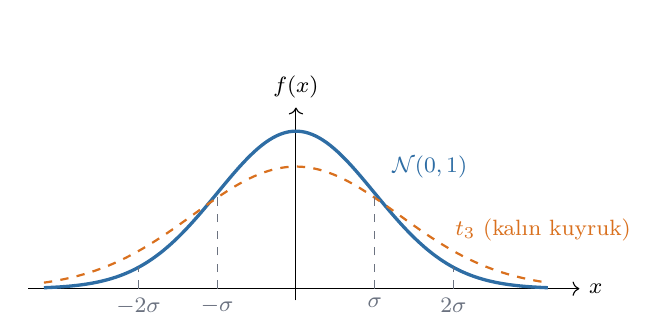
\begin{tikzpicture}[scale=1.0]
\draw[->] (-3.4,0)--(3.6,0) node[right]{\footnotesize $x$};
\draw[->] (0,-0.15)--(0,2.3) node[above]{\footnotesize $f(x)$};
\draw[grafikMavi,very thick,domain=-3.2:3.2,samples=140]
  plot (\x,{2.0*exp(-\x*\x/2)});
\draw[turuncu,thick,dashed,domain=-3.2:3.2,samples=140]
  plot (\x,{1.55*exp(-\x*\x/3.4)});
\node[grafikMavi,right] at (1.1,1.55) {\footnotesize $\mathcal{N}(0,1)$};
\node[turuncu,right] at (1.9,0.75) {\footnotesize $t_3$ (kalın kuyruk)};
\foreach \k/\lbl in {1/{$\sigma$},2/{$2\sigma$}}{
  \draw[dashed,ortaGri] (\k,0)--(\k,{2.0*exp(-\k*\k/2)});
  \draw[dashed,ortaGri] (-\k,0)--(-\k,{2.0*exp(-\k*\k/2)});
}
\node[ortaGri,below] at (1,0) {\footnotesize $\sigma$};
\node[ortaGri,below] at (2,0) {\footnotesize $2\sigma$};
\node[ortaGri,below] at (-1,0) {\footnotesize $-\sigma$};
\node[ortaGri,below] at (-2,0) {\footnotesize $-2\sigma$};
\end{tikzpicture}
\end{center}

\gsub{Gerçek Veriye Dağılım Uydurmak}

\nicin[Normallik Testleri Ne Yapar, Ne Yapmaz?]{Aşağıdaki üç test de aynı
$H_0$'ı sınar: ``bu veri normal dağılımdan geliyor.'' Farkları, dağılımın
neresine baktıklarıdır:
\begin{itemize}\itemsep1pt
\item \textbf{Kolmogorov--Smirnov:} Gözlenen birikimli dağılım ile teorik
CDF arasındaki \emph{en büyük dikey farka} bakar. Genel amaçlıdır ama
kuyruklarda duyarsızdır.
\item \textbf{Shapiro--Wilk:} Özellikle normallik için tasarlanmıştır ve
küçük örneklemlerde en güçlü testtir. Varsayılan tercih budur.
\item \textbf{Anderson--Darling:} Kuyruklara ağırlık verir. Uç değerlerin
önemli olduğu durumlarda (risk analizi, sigortacılık) daha uygundur.
\end{itemize}

\textbf{Niçin normalliği umursuyoruz?} Çünkü $t$-testi, ANOVA, doğrusal
regresyonun güven aralıkları ve $p$-değerleri normallik varsayımı üzerine
kuruludur. Ama --- kritik nokta --- bu yöntemler \emph{verinin} değil,
\emph{istatistiğin} normalliğini gerektirir ve MLT bunu büyük örneklemlerde
zaten sağlar.

\textbf{Bu testlerin büyük tuzağı.} Örneklem büyüdükçe testler \emph{her}
sapmayı yakalar. $n=5000$'de, pratikte normalden ayırt edilemeyecek bir veri
bile $p<0{,}001$ ile reddedilir. Tersine $n=15$'te, açıkça çarpık bir veri
bile reddedilmez --- test zayıftır. Yani normallik testi, tam da ona en çok
ihtiyaç duyduğun küçük örneklemde işe yaramaz, hiç gerekmediği büyük
örneklemde ise sürekli alarm verir.

\textbf{O hâlde ne yapmalı?} \emph{Teste değil grafiğe bak.} Q--Q grafiği
sana yalnızca ``normal mi?'' değil, \emph{nasıl} normal olmadığını da
gösterir: noktalar S çiziyorsa çarpıklık, uçlarda kıvrılıyorsa kalın kuyruk,
basamaklıysa kesikli veri var demektir. Sonra sor: ``bu sapma, kullanacağım
yöntemi gerçekten bozar mı?'' Çoğu zaman cevap hayırdır.

\textbf{Nerede gerçekten kullanılır?} Süreç yeterlilik analizinde (kalite
kontrolde $C_{pk}$ hesabı normallik gerektirir); finansal risk modellerinde
kalın kuyruk tespitinde; ve bir dağılıma parametrik model uydurmadan önce
uyum kontrolünde.}

\begin{lstlisting}
import seaborn as sns
peng = sns.load_dataset('penguins').dropna()
x = peng['body_mass_g']

mu, sd = st.norm.fit(x)                       # maksimum olabilirlik tahmini
print(f"MLE: mu = {mu:.1f}   sigma = {sd:.1f}")

# Uyum iyiligi: uc farkli test
ks = st.kstest(x, st.norm(mu, sd).cdf)
print(f"Kolmogorov-Smirnov: D = {ks.statistic:.4f}  p = {ks.pvalue:.4f}")
sh = st.shapiro(x)
print(f"Shapiro-Wilk:       W = {sh.statistic:.4f}  p = {sh.pvalue:.2e}")
ad = st.anderson(x, 'norm')
print(f"Anderson-Darling:   A2 = {ad.statistic:.3f}  kritik(%5) = {ad.critical_values[2]}")
\end{lstlisting}

\begin{lstlisting}[style=outstyle]
MLE: mu = 4207.1   sigma = 804.0
Kolmogorov-Smirnov: D = 0.1059  p = 0.0010
Shapiro-Wilk:       W = 0.9580  p = 3.57e-08
Anderson-Darling:   A2 = 4.615  kritik(%5) = 0.75
\end{lstlisting}

\uyari{Üç test de normalliği reddediyor --- ama bu, ``normal varsayan hiçbir
yöntem kullanılamaz'' demek değildir. Büyük örneklemlerde normallik testleri
\emph{önemsiz} sapmaları bile yakalar; $n=333$'te kalın kuyruk olmasa da
iki tepelilik (Kısım 2'de gördüğümüz tür karışımı) reddettirir. Doğru
yaklaşım: teste değil, \textbf{Q--Q grafiğine} ve yöntemin sağlamlığına bak.
$t$-testi ve ANOVA, Merkezi Limit Teoremi sayesinde $n>30$'da normallikten
sapmalara oldukça dayanıklıdır.}

\begin{lstlisting}
import matplotlib.pyplot as plt
fig, (a1, a2) = plt.subplots(1, 2, figsize=(11, 4))
sns.histplot(x, kde=True, stat='density', ax=a1, color='#2E6DA4')
xs = np.linspace(x.min(), x.max(), 200)
a1.plot(xs, st.norm(mu, sd).pdf(xs), 'r--', lw=2, label='normal uyum')
a1.legend(); a1.set_title('Histogram + uydurulan normal')
st.probplot(x, dist='norm', plot=a2)          # Q-Q grafigi
a2.set_title('Q-Q grafigi')
plt.tight_layout(); plt.show()
\end{lstlisting}

\gsub{Çarpık Veri: Log-normal Dönüşüm}

\begin{lstlisting}
tit = sns.load_dataset('titanic')
fare = tit.loc[tit.fare > 0, 'fare']
print(f"n={len(fare)}  mean={fare.mean():.2f}  median={fare.median():.2f}  "
      f"skew={fare.skew():.2f}")

s_, loc_, scale_ = st.lognorm.fit(fare, floc=0)
print(f"lognormal uyum: s = {s_:.3f}  scale = {scale_:.2f}  -> mu = {np.log(scale_):.3f}")
print(f"log(fare) carpikligi = {np.log(fare).skew():.3f}")
\end{lstlisting}

\begin{lstlisting}[style=outstyle]
n=876  mean=32.76  median=14.50  skew=4.77
lognormal uyum: s = 0.936  scale = 18.98  -> mu = 2.943
log(fare) carpikligi = 0.901
\end{lstlisting}

\bilgi{Bilet ücretinin çarpıklığı $4{,}77$ (aşırı sağa çarpık); logaritmasını
alınca $0{,}90$'a iniyor. \textbf{Log dönüşümü} çarpımsal süreçlerin
(fiyat, gelir, nüfus, süre) standart tedavisidir: çarpımsal etkileri
toplamsal hâle getirir, varyansı dengeler ve doğrusal modellerin
varsayımlarını sağlar. Sıfır değerler varsa \code{np.log1p} kullan.}

% =====================================================================
\gsec{Büyük Sayılar Yasası ve Merkezi Limit Teoremi}
% =====================================================================

\teorem[Büyük Sayılar Yasası (BSY)]{$X_1,\dots,X_n \iid$ ve $\E[X]=\mu$ sonlu
ise
\[
\bar{X}_n\xrightarrow{\ \Prob\ }\mu \qquad (n\to\infty).
\]
Örneklem ortalaması, anakütle ortalamasına yakınsar.}

\nicin{\textbf{BSY ne diyor?} ``Yeterince çok ölçersen, ortalaman gerçeğe
yaklaşır.'' Kulağa apaçık geliyor --- ama bu, \textbf{tüm istatistiğin
varlık sebebidir}. Eğer bu teorem doğru olmasaydı, bir örneklemden anakütle
hakkında hiçbir şey söyleyemezdik; anket yapmanın, A/B testinin, model
eğitmenin hiçbir anlamı olmazdı.

\textbf{Nerede işe yarar?}
\begin{itemize}\itemsep1pt
\item \textbf{Simülasyon:} Monte Carlo yönteminin tamamı BSY'ye dayanır ---
$\pi$'yi rastgele nokta atarak hesaplayabilmemizin sebebi budur.
\item \textbf{Kumarhane ekonomisi:} Tek bir masada kasa kaybedebilir; ama
milyonlarca el sonunda ortalama, teorik beklenen değere yakınsar. Kasanın
kârı şansa değil, BSY'ye dayanır.
\item \textbf{Sigortacılık:} Tek bir poliçe sahibinin hasarı öngörülemez;
500.000 poliçenin ortalama hasarı ise şaşırtıcı doğrulukla öngörülebilir.
Sigortacılığın iş modeli budur.
\item \textbf{Model değerlendirme:} Test kümesi büyüdükçe ölçtüğün doğruluk,
gerçek performansa yakınsar. 50 örneklik test kümesiyle ölçülen \%92
doğruluk gürültüdür; 50.000 örnekle ölçülen \%92 bilgidir.
\end{itemize}

}

\uyari{\textbf{Kumarbaz yanılgısı --- BSY'nin en yaygın yanlış okunuşu.}
Rulette arka arkaya 10 kez kırmızı geldi; ``artık siyah gelmeli, denge
kurulmalı'' düşüncesi yanlıştır. BSY, geçmişin \emph{telafi edileceğini}
söylemez --- gelecekteki milyonlarca atışın o 10 atışı \emph{seyrelteceğini}
söyler. Çark hafızasızdır. Aynı hata veri biliminde de görülür:
``son üç aydır dönüşüm oranımız düşük, ortalamaya döner'' cümlesi ancak
altta yatan süreç değişmediyse doğrudur.}

\begin{lstlisting}
rng = np.random.default_rng(7)
for n in [10, 100, 1000, 10_000, 100_000]:
    s = rng.integers(1, 7, n)                 # adil zar, gercek ortalama 3.5
    print(f"n = {n:>6}: ortalama = {s.mean():.4f}")
\end{lstlisting}

\begin{lstlisting}[style=outstyle]
n =     10: ortalama = 4.1000
n =    100: ortalama = 3.5900
n =   1000: ortalama = 3.5340
n =  10000: ortalama = 3.4953
n = 100000: ortalama = 3.5065
\end{lstlisting}

\teorem[Merkezi Limit Teoremi (MLT)]{$X_i \iid$, $\E[X]=\mu$,
$\Var(X)=\sigma^2<\infty$ ise \emph{dağılım ne olursa olsun}
\[
\frac{\bar{X}_n-\mu}{\sigma/\sqrt{n}}\ \xrightarrow{\ d\ }\ \mathcal{N}(0,1).
\]
Ortalamanın standart sapması --- \textbf{standart hata} --- $\sigma/\sqrt{n}$
olarak küçülür.}

\nicin{\textbf{MLT niçin ``merkezi''?} Adındaki ``merkezi'' kelimesi
``ortalama'' anlamında değil, \emph{``temel, merkezî öneme sahip''}
anlamındadır --- ve haklı olarak. Söylediği şu: elindeki verinin dağılımı ne
olursa olsun (çarpık, iki tepeli, kesikli, ne olursa), yeterince gözlemin
\emph{ortalaması} normal dağılır.

\textbf{Bu niçin mucize gibi?} Yukarıdaki kodda anakütle üstel dağılımlı ---
son derece çarpık, hiç normale benzemiyor (çarpıklık 1,99). Ama 100'erlik
gruplar alıp ortalamalarına baktığında çarpıklık 0,23'e düşüyor ve elinde
neredeyse mükemmel bir çan eğrisi kalıyor. Verinin şekli hakkındaki bilgi
\emph{buharlaşıyor} ve geriye yalnızca iki sayı kalıyor: $\mu$ ve
$\sigma/\sqrt{n}$.

\textbf{Pratik sonucu nedir?} Bu teorem sayesinde:
\begin{itemize}\itemsep1pt
\item Gelir gibi aşırı çarpık bir veride bile \emph{ortalama gelir} için
normal tabanlı güven aralığı kurabilirsin.
\item $t$-testi, ANOVA, regresyonun $p$-değerleri --- hepsi ``veri normal''
değil, ``\emph{istatistik} normal'' varsayımına dayanır ve MLT bunu sağlar.
\item Bir A/B testinde dönüşüm oranı 0/1 gibi kesikli bir veriden gelir; yine
de ortalamalarının farkı normal kabul edilebilir.
\end{itemize}

\textbf{$\sqrt{n}$ niçin bu kadar önemli?} Standart hatanın $\sigma/\sqrt{n}$
olması, \textbf{belirsizliği yarıya indirmek için örneklemi dört katına
çıkarman gerektiği} anlamına gelir. Bu, veri toplamanın ekonomisini belirleyen
tek formüldür: 400 kişilik bir ankette hata payı $\pm\%5$ ise, $\pm\%2{,}5$
istiyorsan 1600 kişi gerekir --- bütçe dört katına çıkar. Aynı sebeple bir
modelin doğruluğunu \%1 daha hassas ölçmek için test kümesini büyütmek
hızla pahalılaşır.}

\gercek[Anket Sonuçlarındaki ``$\pm$3 Puan'' Nereden Geliyor?]{Seçim
anketlerinde hep aynı cümleyi görürsün: ``1000 kişiyle görüşüldü, hata payı
$\pm3$ puan.'' Bu sayı doğrudan MLT'den gelir.

Bir oranın standart hatası $\sqrt{p(1-p)/n}$'dir ve $p=0{,}5$'te en büyük
değerini alır: $\sqrt{0{,}25/1000}=0{,}0158$. \%95 güven için bunu $1{,}96$
ile çarparsın: $0{,}031$, yani $\pm3{,}1$ puan. Anketi kim yaparsa yapsın,
hangi ülkede olursa olsun, 1000 kişiyle hata payı hep budur.

\textbf{Buradan çıkan iki pratik ders:} (1) İki adayın farkı 2 puansa,
anket ``başa baş'' demektir --- manşetler bunu sürekli yanlış okur.
(2) Hata payı \emph{anakütle büyüklüğüne bağlı değildir}. 80 milyonluk bir
ülkeyi de, 8 milyonluk bir şehri de 1000 kişiyle aynı hassasiyette ölçersin.
Formülde $N$ yok, yalnızca $n$ var. Çorbanın tuzunu anlamak için bir kaşık
yeter --- tencerenin büyüklüğü fark etmez, yeter ki iyice karıştırılmış
olsun (\emph{rastgele örnekleme}).}

\begin{lstlisting}
rng = np.random.default_rng(1)
pop = rng.exponential(scale=2.0, size=1_000_000)       # ustel: cok carpik
print(f"anakutle: mean={pop.mean():.3f} std={pop.std():.3f} "
      f"skew={st.skew(pop):.3f}")

for n in [1, 5, 30, 100]:
    means = rng.choice(pop, size=(20_000, n)).mean(axis=1)
    print(f"n={n:>4}: ort={means.mean():.3f}  std={means.std():.4f}  "
          f"teorik SE={pop.std()/np.sqrt(n):.4f}  carpiklik={st.skew(means):+.3f}")
\end{lstlisting}

\begin{lstlisting}[style=outstyle]
anakutle: mean=1.996 std=1.992 skew=1.989
n=   1: ort=2.003  std=2.0013  teorik SE=1.9922  carpiklik=+1.966
n=   5: ort=1.996  std=0.8901  teorik SE=0.8909  carpiklik=+0.877
n=  30: ort=1.996  std=0.3619  teorik SE=0.3637  carpiklik=+0.353
n= 100: ort=1.998  std=0.1987  teorik SE=0.1992  carpiklik=+0.227
\end{lstlisting}

\bilgi{Anakütle çarpıklığı $1{,}99$ iken, 100'lük ortalamaların çarpıklığı
$0{,}23$'e düşüyor ve standart sapma teorik $\sigma/\sqrt{n}$ ile neredeyse
tam örtüşüyor. \textbf{MLT bu rehberdeki her güven aralığının ve $t$-testinin
temelidir}: veri normal olmasa bile \emph{ortalaması} yaklaşık normaldir.}

\uyari{MLT'nin iki sınırı vardır: (1) $\sigma^2$ sonlu olmalıdır --- Cauchy
gibi dağılımlarda MLT geçerli değildir; (2) yakınsama hızı çarpıklığa
bağlıdır. Kaba kural $n>30$'dur ama çok çarpık dağılımlarda $n>200$ bile
gerekebilir. Emin değilsen bootstrap kullan (Kısım 5).}

% =====================================================================
\gsec{Monte Carlo ve Örnekleme Yöntemleri}
% =====================================================================

\nicin[Fikir Nedir?]{Monte Carlo yönteminin tek cümlelik özeti şudur:
\textbf{``Hesaplayamıyorsan, simüle et.''} Bir olasılığı, integrali ya da
beklenen değeri analitik olarak çözmek yerine, süreci binlerce kez taklit
edip sonuçların ortalamasını alırsın. BSY bu ortalamanın doğru cevaba
yakınsayacağını garanti eder.

Aşağıdaki $\pi$ örneği fikri çıplak hâliyle gösteriyor: birim kareye rastgele
nokta at, çeyrek daire içine düşenlerin oranını bul, 4 ile çarp. Hiç geometri
bilmene gerek yok --- yalnızca rastgele sayı üretebilmen yeter.

\textbf{Niçin bu kadar kullanışlı?} Çünkü gerçek problemlerin çoğunun
analitik çözümü \emph{yoktur}. Formül yazılamayan yerde simülasyon her zaman
çalışır. Ayrıca simülasyon kurmak, formül türetmekten çok daha az hata
yapılan bir iştir --- kodun kendisi modelin tarifidir.

\textbf{Nerede kullanılır?}
\begin{itemize}\itemsep1pt
\item \textbf{Finans:} Opsiyon fiyatlaması, portföy riski (VaR). ``Bu portföy
1 yılda en kötü \%1 senaryoda ne kaybeder?'' sorusu 100.000 fiyat yolu
simüle edilerek cevaplanır.
\item \textbf{Proje planlama:} Her görevin süresi belirsizse, projenin
toplam süresi için tek bir sayı değil bir \emph{dağılım} elde edersin
(``\%90 ihtimalle 14 haftadan önce biter'').
\item \textbf{Mühendislik:} Tolerans yığılması --- 12 parçanın her birinin
üretim toleransı verildiğinde montajın toplam sapması.
\item \textbf{İstatistik:} Bootstrap (Kısım 5), permütasyon testi (Kısım 6),
Bayesçi MCMC --- üçü de birer Monte Carlo uygulamasıdır.
\item \textbf{Yapay zekâ:} Monte Carlo Ağaç Araması (MCTS), AlphaGo'nun
temel algoritmasıdır: hangi hamlenin iyi olduğunu hesaplamak yerine, o
hamleden sonra binlerce oyunu rastgele oynatıp kazanma oranına bakar.
\end{itemize}}

\begin{lstlisting}
rng = np.random.default_rng(3)
for n in [10**3, 10**4, 10**5, 10**6]:
    p = rng.random((n, 2))
    pi = 4*np.mean((p**2).sum(axis=1) <= 1)
    print(f"n = {n:>8}: pi ~ {pi:.5f}   hata = {abs(pi - np.pi):.5f}")
\end{lstlisting}

\begin{lstlisting}[style=outstyle]
n =     1000: pi ~ 3.13200   hata = 0.00959
n =    10000: pi ~ 3.12800   hata = 0.01359
n =   100000: pi ~ 3.13508   hata = 0.00651
n =  1000000: pi ~ 3.14135   hata = 0.00024
\end{lstlisting}

\form[Monte Carlo Yakınsama Hızı]{Hata $O(1/\sqrt{n})$ ile azalır: basamak
kazanmak için örnek sayısını \emph{100 katına} çıkarman gerekir. Yavaştır ama
boyuttan bağımsızdır --- bu yüzden yüksek boyutlu integrallerde tek pratik
yöntemdir.}

\nicin{\textbf{``Boyuttan bağımsız'' niçin bu kadar önemli?} Klasik sayısal
integrasyon (yamuk kuralı, Simpson) tek boyutta Monte Carlo'dan çok daha
hızlıdır. Ama $d$ boyutta ızgara kurmak için her eksende $m$ nokta gerekir,
yani $m^d$ hesap --- 10 boyutta ve eksen başına 100 noktada bu
$10^{20}$ eder, imkânsız. Buna \textbf{boyut laneti} denir.

Monte Carlo'nun hatası ise $O(1/\sqrt{n})$'dir ve bu ifadede $d$ \emph{yoktur}.
1 boyutta da 100 boyutta da aynı yavaşlıkta yakınsar. Yavaş ama boyuta
duyarsız olması, yüksek boyutlu problemlerde onu tek seçenek hâline getirir ---
ve makine öğrenmesindeki hemen her problem yüksek boyutludur.

\textbf{Pratik okuma:} Sonucunun ilk basamağını doğru istiyorsan $\sim100$
örnek, iki basamak için $\sim10\,000$, üç basamak için $\sim10^6$ örnek
gerekir. Bu yüzden bootstrap'ta 1000--10.000 tekrar standarttır: karar
vermek için gereken hassasiyet zaten o civardadır, daha fazlası boşa
hesaptır.}

\gsub{Ters Dönüşüm ve Kabul-Ret Yöntemleri}

\begin{lstlisting}
# 1) Ters donusum: U ~ Uniform(0,1) ise F^{-1}(U) ~ F
u = rng.random(100_000)
ustel = -np.log(1 - u)/0.5                    # Exp(lambda=0.5)
print(f"ortalama = {ustel.mean():.3f}")     # 1.998  (teorik 2.0)

# 2) Kabul-ret: hedef yogunluk f, onerici g, f <= M*g
def kabul_ret(f, n, a=0, b=1, M=2.0, rng=rng):
    kabul = []
    while len(kabul) < n:
        x = rng.uniform(a, b, n)
        u = rng.random(n)
        kabul.extend(x[u < f(x)/M])
    return np.array(kabul[:n])

ornek = kabul_ret(lambda x: 2*x, 50_000)      # f(x) = 2x, 0<x<1
print(f"ortalama = {ornek.mean():.4f}")    # 0.6664  (teorik 2/3)
\end{lstlisting}

\ipucu{\code{numpy.random} zaten tüm standart dağılımlar için hızlı üreteçlere
sahiptir; ters dönüşüm ve kabul-ret yöntemlerini \emph{öğrenmek} için değil,
\emph{standart olmayan} bir dağılımdan örnekleme gerektiğinde kullanırsın.
Bayesçi çıkarımda (Kısım 6) aynı fikir MCMC'ye dönüşür.}

% #####################################################################
\gpart{5}{Çıkarımsal İstatistik: Tahmin}
% #####################################################################

% =====================================================================
\gsec{Örnekleme Dağılımı ve Standart Hata}
% =====================================================================

Elimizde \emph{anakütle} değil \emph{örneklem} vardır. Örneklemden hesapladığımız
her istatistik ($\bar{x}$, $s$, $r$, $\hat{p}$\dots) bir rastgele değişkendir ve
kendi dağılımına sahiptir: \textbf{örnekleme dağılımı}.

\nicin[Bu Kısım Niçin Var?]{Buraya kadar veriyi \emph{betimledik} (Kısım 2)
ve belirsizliğin dilini kurduk (Kısım 3--4). Şimdi asıl soruya geliyoruz:
\textbf{elimizdeki 333 penguenden, dünyadaki bütün penguenler hakkında ne
söyleyebiliriz?} Bu sıçramaya \emph{çıkarım} denir ve istatistiğin var oluş
sebebidir.

Sıçramanın bedeli belirsizliktir. 333 penguenin ortalaması 4207 g çıktı ---
ama başka 333 penguen ölçseydik 4180 ya da 4240 çıkardı. İşte
\textbf{örnekleme dağılımı}, ``bu deneyi tekrar tekrar yapsaydım
hesapladığım sayı nasıl oynardı?'' sorusunun cevabıdır. Bu kısımdaki her
şey --- standart hata, güven aralığı, bootstrap --- o oynamanın büyüklüğünü
ölçmenin farklı yollarıdır.

\textbf{Üç dağılımı asla karıştırma:} (1) \emph{Anakütle dağılımı} --- tüm
penguenlerin ağırlıkları. (2) \emph{Örneklem dağılımı} --- elindeki 333
gözlemin histogramı. (3) \emph{Örnekleme dağılımı} --- tekrarlanan
örneklemlerden hesaplanan \emph{ortalamaların} dağılımı. Üçüncüsü hayalîdir,
onu asla göremezsin --- ama Merkezi Limit Teoremi şeklini, standart hata
genişliğini verir. Çıkarımın tamamı bu görünmez dağılım üzerine kuruludur.}

\form[Standart Hata]{Bir istatistiğin örnekleme dağılımının standart sapmasına
\emph{standart hata} denir. Ortalama için:
\[
\mathrm{SE}(\bar{X})=\frac{\sigma}{\sqrt{n}}\ \approx\ \frac{s}{\sqrt{n}} .
\]
\textbf{Standart sapma} verinin yayılımını, \textbf{standart hata} tahminin
belirsizliğini ölçer. İkisini karıştırmak, bilimsel makalelerdeki en yaygın
hatadır.}

\nicin{\textbf{Farkı bir cümlede:} Standart sapma \emph{penguenler} hakkında,
standart hata \emph{senin ölçümün} hakkındadır.

Somutlaştıralım: $s=805$ g, ``penguenler birbirinden ne kadar farklı?''
sorusunu cevaplar --- ve daha çok penguen ölçersen bu sayı \emph{değişmez},
çünkü penguenlerin çeşitliliği senin kaç tane ölçtüğüne bağlı değildir.
$\mathrm{SE}=44$ g ise ``hesapladığım 4207 rakamı ne kadar güvenilir?''
sorusunu cevaplar --- ve $n$ büyüdükçe \emph{sıfıra gider}, çünkü daha çok
ölçüm daha kesin bir ortalama demektir.

\textbf{Niçin karıştırmak ciddi bir hata?} Bir grafikte hata çubuklarını
$\pm s$ yerine $\pm\mathrm{SE}$ çizersen çubuklar $\sqrt{n}$ kat daha kısa
görünür; iki grubun çubukları ayrışmış gibi durur ve okuyucu var olmayan bir
fark görür. Bilimsel dergilerin ``hata çubuğunun neyi gösterdiğini yazın''
diye ısrar etmesinin sebebi budur.

\textbf{Hangisini ne zaman raporlarsın?}
\begin{itemize}\itemsep1pt
\item \emph{Bireylerin çeşitliliğini} anlatıyorsan ($s$): ``Hastaların kan
basıncı 120$\pm$15 mmHg aralığında değişiyor.'' Bir sonraki hastanın nerede
olacağını tahmin etmek için bu gerekir.
\item \emph{Tahmininin kesinliğini} anlatıyorsan (SE): ``Ortalama kan basıncı
120$\pm$1,5 mmHg.'' Güven aralığı, hipotez testi, A/B testi kararı --- hepsi
SE ile çalışır.
\end{itemize}

\textbf{Nerede karşına çıkar?} Anketlerdeki ``hata payı''; regresyon
çıktısındaki her katsayının yanındaki \code{std err} sütunu; makine
öğrenmesinde çapraz doğrulama skorlarının $\pm$'si; ilaç denemelerinde etki
büyüklüğünün güven aralığı. Hepsi standart hatadır.}

\begin{lstlisting}
import numpy as np, seaborn as sns
peng = sns.load_dataset('penguins').dropna()
x = peng['body_mass_g'].to_numpy()
n = len(x)

print(f"n = {n}")
print(f"ortalama = {x.mean():.1f} g")
print(f"std      = {x.std(ddof=1):.1f} g       <- verinin yayilimi")
print(f"SE       = {x.std(ddof=1)/np.sqrt(n):.2f} g    <- tahminin belirsizligi")
\end{lstlisting}

\begin{lstlisting}[style=outstyle]
n = 333
ortalama = 4207.1 g
std      = 805.2 g       <- verinin yayilimi
SE       = 44.13 g    <- tahminin belirsizligi
\end{lstlisting}

\uyari{$\sqrt{n}$ kuralı acımasızdır: belirsizliği yarıya indirmek için
örneklemi \textbf{dört katına} çıkarman gerekir. 333 penguen yerine 1332
penguen ölçersen SE $44{,}13\to22{,}07$'ye iner. Bu, deney tasarımında
maliyetin neden hızla arttığının matematiksel nedenidir.}

% =====================================================================
\gsec{Nokta Tahmini: MLE ve Momentler Yöntemi}
% =====================================================================

\form[Maksimum Olabilirlik (MLE)]{Veriyi \emph{en olası} kılan parametreyi
seç:
\[
\hat{\theta}_{\text{MLE}}=\arg\max_\theta \mathcal{L}(\theta\mid x)
=\arg\max_\theta \prod_i f(x_i\mid\theta)
=\arg\max_\theta \sum_i \log f(x_i\mid\theta).
\]
Çarpım yerine logaritma toplamı kullanılır: hem sayısal taşmayı önler hem de
türev almayı kolaylaştırır.}

\nicin{\textbf{Fikir nedir?} Elinde veri var, ama onu üreten parametreyi
bilmiyorsun. MLE şu soruyu sorar: \emph{``Hangi parametre değeri, tam olarak
bu veriyi görme ihtimalimi en yüksek yapar?''} Yani mantığı tersine çevirir:
normalde parametreden veriye gideriz, MLE veriden parametreye gider.

\textbf{Somut örnek.} Bir madenî parayı 10 kez attın, 7 tura geldi. Tura
olasılığı $p$ nedir? $p=0{,}1$ olsaydı bu sonucu görme şansın binde bir bile
değil; $p=0{,}9$ olsaydı da düşük. $p=0{,}7$'de olabilirlik en yüksek çıkar.
MLE cevabı $\hat p=0{,}7$'dir --- ve bu, sezgisel olarak yapacağın şeyin ta
kendisidir. MLE'nin güzelliği, bu sezgiyi \emph{her} dağılım için işleyen bir
tarife dönüştürmesidir.

\textbf{Olabilirlik ile olasılık aynı şey değildir.} Olasılıkta parametre
sabit, veri değişkendir (``$p=0{,}5$ ise 7 tura gelme olasılığı?''). Olabilirlikte
veri sabit, parametre değişkendir (``7 tura gördüm, hangi $p$ bunu en olası
kılar?''). $\mathcal{L}(\theta\mid x)$ bir olasılık dağılımı \emph{değildir};
$\theta$ üzerinden integrali 1 etmez.

\textbf{Niçin logaritma?} İki sebep: (1) 1000 gözlemin olasılıklarını
çarparsan sonuç $10^{-3000}$ mertebesinde olur ve bilgisayarda sıfıra
yuvarlanır (\emph{underflow}); logaritma bunu toplamaya çevirip sorunu
bitirir. (2) Türev almak çarpımda zincir kuralı yığını demektir, toplamda ise
terim terim türevdir. Kayıp fonksiyonlarının hep ``log'' ile başlamasının
sebebi budur.

\textbf{Nerede kullanılır --- yani neredeyse her yerde:}
\begin{itemize}\itemsep1pt
\item \textbf{Lojistik regresyon} tam olarak MLE ile eğitilir; minimize
ettiği \emph{log-loss} (çapraz entropi), negatif log-olabilirliktir.
\item \textbf{Doğrusal regresyon:} Hataların normal olduğu varsayımı altında
MLE, en küçük kareler yöntemiyle \emph{birebir aynı} sonucu verir. ``Kareleri
niçin topluyoruz?'' sorusunun gerçek cevabı budur.
\item \textbf{Sinir ağları:} Sınıflandırmada çapraz entropi, regresyonda MSE
kaybı --- ikisi de negatif log-olabilirliktir. Bir ağı eğitmek, MLE yapmaktır.
\item \textbf{Dağılım uydurma:} \code{scipy}'deki \code{dist.fit(data)}
çağrısı MLE çalıştırır.
\item \textbf{Zaman serileri:} ARIMA, GARCH ve durum-uzayı modelleri MLE ile
kestirilir.
\end{itemize}}

\gercek[Kayıp Uçağı MLE ile Aramak]{Bir hava aracının son bilinen konumu ve
hız verileri var. ``Nereye düştü?'' sorusu bir MLE problemidir: her olası
düşüş noktası için ``bu nokta doğruysa, elimdeki radar ve uydu sinyallerini
görme olabilirliğim ne?'' hesaplanır; olabilirliği en yüksek nokta arama
merkezine seçilir.

Aynı mantığı her gün kullanan bir sistem daha var: telefonundaki
\textbf{GPS}. Uydulardan gelen sinyal süreleri gürültülüdür; alıcı, ``hangi
konum bu ölçüm setini en olası kılar?'' sorusunu çözerek konumunu bulur.
Konum bulma, gizli bir MLE'dir.}

\gsubsub{Normal dağılım için türetim}

$\log\mathcal{L}=-\frac{n}{2}\log(2\pi\sigma^2)-\frac{1}{2\sigma^2}\sum(x_i-\mu)^2$
ifadesinin türevlerini sıfıra eşitlersek:
\[
\frac{\partial}{\partial\mu}: \sum(x_i-\mu)=0 \Rightarrow \hat{\mu}=\bar{x},
\qquad
\frac{\partial}{\partial\sigma^2}: \hat{\sigma}^2=\frac{1}{n}\sum(x_i-\bar{x})^2 .
\]
Dikkat: MLE varyans tahmini $n$'e böler, yani \textbf{yanlıdır}.

\begin{lstlisting}
from scipy import stats as st
from scipy.optimize import minimize

def neg_loglik(params, data):
    mu, log_sigma = params                    # log_sigma: sigma>0 kisitini kaldirir
    return -np.sum(st.norm.logpdf(data, mu, np.exp(log_sigma)))

res = minimize(neg_loglik, x0=[4000, np.log(500)], args=(x,), method='Nelder-Mead')
print(f"sayisal MLE : mu = {res.x[0]:.2f}   sigma = {np.exp(res.x[1]):.2f}")
print(f"kapali form : mu = {x.mean():.2f}   sigma = {x.std(ddof=0):.2f}")
\end{lstlisting}

\begin{lstlisting}[style=outstyle]
sayisal MLE : mu = 4207.06   sigma = 804.01
kapali form : mu = 4207.06   sigma = 804.01
\end{lstlisting}

\form[Momentler Yöntemi]{Teorik momentleri örneklem momentlerine eşitle:
$\E[X]=\bar{x}$, $\E[X^2]=\overline{x^2}$, \dots\ MLE'den daha basit ama
genellikle daha az verimlidir. Bazı dağılımlarda (örn.\ gamma) hızlı bir
başlangıç değeri üretmek için kullanılır.}

\nicin{\textbf{Fikir çok basit:} Dağılımın teorik ortalaması $\mu(\theta)$
parametreye bağlıdır. Elindeki verinin ortalaması $\bar{x}$ ise, ``bu ikisi
eşit olsun'' deyip $\theta$'yı çöz. Kaç parametre varsa o kadar moment
denklemi yazarsın.

\emph{Örnek:} Bir üstel dağılımda $\E[X]=1/\lambda$'dır. Bekleme süreleri
ortalaman 4 dakikaysa $\hat\lambda=1/4$ dersin. Bitti --- optimizasyon yok,
türev yok.

\textbf{Niçin MLE varken buna ihtiyaç var?} Üç durumda:
(1) MLE'nin kapalı çözümü yoksa ve sayısal optimizasyon bir başlangıç noktası
istiyorsa (gamma dağılımı klasik örnektir);
(2) MLE hesaplaması çok pahalıysa ve kaba bir tahmin yeterliyse;
(3) Dağılımın tam biçimini varsaymak istemeyip yalnızca momentlere
dayanmak istediğinde --- ekonometride \emph{Genelleştirilmiş Momentler
Yöntemi} (GMM) bu fikrin ciddi bir genellemesidir ve Nobel getirmiştir.

\textbf{Bedeli ne?} Genellikle MLE'den daha büyük varyanslı tahminler verir,
yani aynı veriden daha az bilgi çıkarır. Bazen anlamsız sonuç bile
üretebilir (parametre tanım aralığının dışına düşebilir). Kural: MLE
hesaplanabiliyorsa MLE kullan.}

\gsub{İyi Bir Tahmin Edici Nedir?}

\begin{center}
\begin{tabularx}{\textwidth}{@{}>{\bfseries\color{anaMavi}}l >{$\displaystyle}l<{$} >{\raggedright\arraybackslash}X@{}}
\toprule
\rowcolor{acikMavi}\multicolumn{1}{@{}l}{\color{anaMavi}\textbf{Özellik}} & \multicolumn{1}{l}{\color{anaMavi}\textbf{Tanım}} & \multicolumn{1}{l@{}}{\color{anaMavi}\textbf{Anlamı}}\\
\midrule
Yansızlık & \E[\hat\theta]=\theta & Ortalamada doğruyu vurur.\\
\rowcolor{acikGri} Tutarlılık & \hat\theta\xrightarrow{\Prob}\theta & $n$ büyüdükçe doğruya yakınsar.\\
Verimlilik & \min \Var(\hat\theta) & Aynı yansızlıkta en küçük varyans.\\
\rowcolor{acikGri} MSE & \E[(\hat\theta-\theta)^2]=\text{yanlılık}^2+\Var & Toplam hata ölçüsü.\\
\bottomrule
\end{tabularx}
\end{center}

\begin{lstlisting}
# Bessel duzeltmesi gercekten yanliligi gideriyor mu? Simule edelim.
rng = np.random.default_rng(42)
b_n, b_n1 = [], []
for _ in range(20_000):
    s = rng.normal(0, 10, 10)                 # gercek varyans = 100
    b_n.append(s.var(ddof=0))                 # n'e bolen
    b_n1.append(s.var(ddof=1))                # n-1'e bolen
print(f"ddof=0 ortalama = {np.mean(b_n):6.2f}   yanlilik = {np.mean(b_n)-100:+.2f}")
print(f"ddof=1 ortalama = {np.mean(b_n1):6.2f}   yanlilik = {np.mean(b_n1)-100:+.2f}")
\end{lstlisting}

\begin{lstlisting}[style=outstyle]
ddof=0 ortalama =  90.57   yanlilik = -9.43
ddof=1 ortalama = 100.63   yanlilik = +0.63
\end{lstlisting}

\bilgi{$n=10$'da $n$'e bölmek varyansı sistematik olarak \%10 küçük tahmin
ediyor --- tam olarak $(n-1)/n=0{,}9$ oranında. Bessel düzeltmesi bunu
gideriyor. \textbf{Yanlılık--varyans dengesi} burada başlar ve Kısım 8'de
makine öğrenmesinin merkezî kavramı olarak geri döner: bazen \emph{yanlı} ama
düşük varyanslı bir tahmin (Ridge regresyonu gibi), yansız ama oynak bir
tahminden daha iyidir.}

% =====================================================================
\gsec{Güven Aralıkları}
% =====================================================================

\form[Ortalama için Güven Aralığı]{
\[
\bar{x}\pm t_{\alpha/2,\,n-1}\cdot\frac{s}{\sqrt{n}}
\]
$\sigma$ bilinmediği için $z$ yerine $t$ dağılımı kullanılır; $n$ büyüdükçe
$t\to z$ olur.}

\nicin{\textbf{Niçin tek bir sayı yetmiyor?} ``Ortalama penguen ağırlığı
4207 g'' cümlesi eksiktir; hiçbir ölçüm sonsuz kesinlikte değildir. Güven
aralığı, tahmine \emph{dürüstlük} ekler: ``4207, ama gerçek değer büyük
olasılıkla 4120 ile 4294 arasında.'' Karar veren kişi için ikinci cümle
birincisinden kat kat kullanışlıdır.

\textbf{Formülün anatomisi.} Üç parça var ve her biri ayrı bir şey söyler:
\begin{itemize}\itemsep1pt
\item $\bar{x}$ --- \emph{en iyi tahminim}, aralığın merkezi.
\item $s/\sqrt{n}$ --- \emph{standart hata}; verinin oynaklığı ve örneklem
büyüklüğü aralığı ne kadar genişletiyor.
\item $t_{\alpha/2,n-1}$ --- \emph{ne kadar emin olmak istiyorum}. \%95 için
$\approx2$, \%99 için $\approx2{,}6$. Daha yüksek güven, daha geniş aralık:
bedava emin olamazsın.
\end{itemize}

\textbf{Niçin $z$ değil $t$?} $\sigma$'yı bilmiyor, onu da aynı veriden
tahmin ediyorsun ($s$). Yani iki katmanlı bir belirsizlik var ve $z$ bunu
hesaba katmaz --- aralığı olduğundan dar verir. $t$ dağılımının normalden
kalın kuyruklu olması tam olarak bu ekstra belirsizliğin telafisidir.
$n=10$'da $t^*=2{,}26$ iken $n=333$'te $2{,}0$'a iner; büyük örneklemde
$s\approx\sigma$ olduğu için fark kapanır.

\textbf{Güven düzeyi nasıl seçilir?} \%95 bir gelenektir, doğa kanunu değil.
Yanlış karar pahalıysa (ilaç onayı, uçak parçası) \%99 kullanılır; keşif
amaçlı analizde \%90 yeterlidir. Seçimi \emph{veriye baktıktan sonra} yapmak
ise ciddi bir usul hatasıdır.

\textbf{Nerede kullanılır?} İlaç etkinliği raporları (``risk azalması
\%23, GA: \%12--\%33''); A/B testi sonuçları; anket hata payları; regresyon
katsayılarının aralıkları; model doğruluğunun çapraz doğrulama aralığı.}

\gercek[Aralık, Nokta Tahmininden Niçin Daha Çok Şey Söyler?]{İki A/B testi
düşün. İkisinde de dönüşüm oranı artışı \textbf{+\%2} çıktı.
\begin{itemize}\itemsep1pt
\item \emph{Test A:} \%95 GA $=[+1{,}8;\ +2{,}2]$. Etki küçük ama
\emph{kesin}. Uygula.
\item \emph{Test B:} \%95 GA $=[-15;\ +19]$. Aynı ``+\%2'' rakamı, ama veri
neredeyse hiçbir şey söylemiyor. Doğru karar: daha fazla veri topla.
\end{itemize}
Yalnızca nokta tahminine bakan bir yönetici bu iki testi \emph{aynı} görür.
Aralık ise ikisi arasındaki uçurumu tek bakışta gösterir.

Aynı sebeple, ``fark anlamlı çıkmadı'' cümlesi de tek başına yetersizdir.
GA $=[-0{,}3;\ +0{,}4]$ ise ``etki yok, kapatalım'' diyebilirsin;
GA $=[-20;\ +25]$ ise doğru cümle ``\emph{henüz bilmiyoruz}''dur. İkisi
arasındaki farkı $p$-değeri gizler, güven aralığı gösterir.}

\begin{lstlisting}
se = x.std(ddof=1)/np.sqrt(n)

t_crit = st.t.ppf(0.975, df=n-1)
print(f"t*  = {t_crit:.4f}")
print(f"t-CI 95%: [{x.mean()-t_crit*se:.1f}, {x.mean()+t_crit*se:.1f}]")

# Kisa yol
lo, hi = st.t.interval(0.95, df=n-1, loc=x.mean(), scale=se)
print(f"scipy   : [{lo:.1f}, {hi:.1f}]")

for lvl in [0.80, 0.90, 0.95, 0.99]:
    lo, hi = st.t.interval(lvl, n-1, x.mean(), se)
    print(f"  %{lvl*100:.0f}: [{lo:.1f}, {hi:.1f}]   genislik = {hi-lo:.1f}")
\end{lstlisting}

\begin{lstlisting}[style=outstyle]
t*  = 1.9671
t-CI 95%: [4120.3, 4293.9]
scipy   : [4120.3, 4293.9]
  %80: [4150.4, 4263.7]   genislik=113.3
  %90: [4134.3, 4279.8]   genislik=145.6
  %95: [4120.3, 4293.9]   genislik=173.6
  %99: [4092.7, 4321.4]   genislik=228.6
\end{lstlisting}

\uyari{\textbf{Güven aralığının doğru yorumu.} ``Gerçek ortalamanın bu
aralıkta olma olasılığı \%95'tir'' cümlesi \emph{yanlıştır} (sıklıkçı
çerçevede gerçek ortalama sabittir, rastgele olan aralıktır). Doğru yorum:
\emph{``Aynı yöntemi tekrar tekrar uygularsam, ürettiğim aralıkların \%95'i
gerçek değeri içerir.''} Aşağıda bunu simüle ediyoruz.}

\begin{lstlisting}
kapsama = 0
M = 10_000
for _ in range(M):
    s = rng.normal(100, 15, 20)               # gercek ortalama = 100
    lo, hi = st.t.interval(0.95, 19, s.mean(), s.std(ddof=1)/np.sqrt(20))
    kapsama += (lo <= 100 <= hi)
print(f"gercek kapsama orani = {kapsama/M:.4f}   (hedef 0.95)")
\end{lstlisting}

\begin{lstlisting}[style=outstyle]
gercek kapsama orani = 0.9507   (hedef 0.95)
\end{lstlisting}

\gsub{Oran için Güven Aralığı}

\begin{lstlisting}
tit = sns.load_dataset('titanic')
k, N = tit.survived.sum(), len(tit)
p = k/N
print(f"p_hat = {p:.4f}   (k={k}, n={N})")

from statsmodels.stats.proportion import proportion_confint
for m in ['normal', 'wilson', 'beta']:
    lo, hi = proportion_confint(k, N, alpha=0.05, method=m)
    print(f"{m:>8}: [{lo:.4f}, {hi:.4f}]")
\end{lstlisting}

\begin{lstlisting}[style=outstyle]
p_hat = 0.3838   (k=342, n=891)
  normal: [0.3519, 0.4158]
  wilson: [0.3525, 0.4162]
    beta: [0.3518, 0.4167]
\end{lstlisting}

\ipucu{\code{normal} (Wald) aralığı $p$ uçlara ($0$ veya $1$) yakınken ya da
$n$ küçükken kötü çalışır --- hatta $[0,1]$ dışına taşabilir. Varsayılan
tercihini \textbf{Wilson} yap; kesin garanti istiyorsan \code{beta}
(Clopper--Pearson) kullan. Bu fark, tıklama oranı (CTR) gibi küçük oranlarda
ciddileşir.}

% =====================================================================
\gsec{Bootstrap: Formülsüz Çıkarım}
% =====================================================================

Bir istatistiğin örnekleme dağılımını formülle bulamıyorsan (medyan,
korelasyon, çeyrekler arası açıklık, R$^2$\dots), veriyi \emph{kendisinden}
yeniden örnekleyerek yaklaş.

\form[Bootstrap Algoritması]{
\begin{enumerate}\itemsep1pt
\item Veriden \emph{iadeli} olarak $n$ gözlem çek.
\item İstatistiği hesapla.
\item 1--2'yi $B$ kez ($B\ge2000$) tekrarla.
\item Elde edilen $B$ değerin dağılımı, örnekleme dağılımının tahminidir;
yüzdelikleri güven aralığını verir.
\end{enumerate}}

\nicin{\textbf{Fikir neden ``imkânsız'' görünüyor?} Bootstrap, adını
``kendi ayakkabı bağcığından tutup kendini havaya kaldırmak'' deyiminden
alır --- çünkü tek bir örneklemden, sanki defalarca örneklem almışsın gibi
bilgi üretir. Mantığı şudur: elindeki örneklem, anakütlenin en iyi
kopyasıdır. O hâlde anakütleden tekrar tekrar örnek çekemiyorsan,
\emph{örnekleminden} tekrar tekrar çek. Anakütle : örneklem ilişkisini,
örneklem : yeniden örneklem ilişkisiyle taklit edersin.

\textbf{İadeli çekmek niçin şart?} İadesiz çekersen her seferinde aynı 333
gözlemi farklı sırayla alırsın ve ortalama hiç değişmez --- hiçbir bilgi
üretmezsin. İade sayesinde bazı gözlemler iki kez girer, bazıları hiç
girmez; işte bu, ``başka bir örneklem çekseydim ne olurdu?'' sorusunun
taklididir.

\textbf{Niçin bu kadar değerli?} Çünkü \emph{formülden kurtarır}. Klasik
istatistik her istatistik için ayrı bir örnekleme dağılımı türetmek zorundadır
ve bu çoğu zaman ya çok zordur ya da imkânsızdır. Bootstrap ise tek bir
tarifle her şeye uygulanır: medyan, çeyrekler açıklığı, korelasyon, $R^2$,
Gini katsayısı, iki grubun medyan farkı, bir makine öğrenmesi modelinin AUC
skoru\dots\ Ortak özellikleri: hiçbirinin kapalı formülü yoktur, hepsinin
bootstrap güven aralığı beş satır kodla hesaplanır.

\textbf{Nerede kullanılır?}
\begin{itemize}\itemsep1pt
\item \textbf{Model belirsizliği:} ``Modelimin AUC'si 0,84'' yerine
``AUC $=0{,}84$, \%95 GA $=[0{,}79;\ 0{,}88]$'' demek --- test kümesini
bootstrap'layarak.
\item \textbf{Topluluk yöntemleri:} Rastgele ormandaki ``bagging'' kelimesi
\emph{bootstrap aggregating}'in kısaltmasıdır. Her ağaç, bootstrap örneği
üzerinde eğitilir; eğitime girmeyen \%36,8'lik kısım (\emph{out-of-bag})
bedava doğrulama kümesi olur.
\item \textbf{İş metrikleri:} ``Müşteri yaşam boyu değerinin medyanı'' gibi
çarpık dağılımlı metriklerde güven aralığı kurmanın pratikteki tek yolu.
\item \textbf{A/B testi:} Metrik ortalama değil de \%90'lık yüzdelik ya da
gelirin medyanı ise, klasik test yoktur --- bootstrap vardır.
\end{itemize}}

\begin{lstlisting}
def boot_ci(data, stat=np.mean, B=10_000, alpha=0.05, rng=rng):
    """Yuzdelik (percentile) bootstrap guven araligi."""
    idx = rng.integers(0, len(data), (B, len(data)))     # iadeli ornekleme
    boots = stat(data[idx], axis=1)
    return np.percentile(boots, [100*alpha/2, 100*(1-alpha/2)]), boots

(lo, hi), boots = boot_ci(x)
print(f"bootstrap ORTALAMA GA: [{lo:.1f}, {hi:.1f}]   (bootstrap SE = {boots.std():.2f})")

(mlo, mhi), _ = boot_ci(x, stat=np.median)
print(f"bootstrap MEDYAN   GA: [{mlo:.1f}, {mhi:.1f}]   <- formulu yok!")

# scipy'nin BCa (yanlilik duzeltmeli) surumu
res = st.bootstrap((x,), np.mean, confidence_level=0.95,
                   n_resamples=10_000, random_state=42)
print(f"scipy BCa            : [{res.confidence_interval.low:.1f}, "
      f"{res.confidence_interval.high:.1f}]")
\end{lstlisting}

\begin{lstlisting}[style=outstyle]
bootstrap ORTALAMA GA: [4122.8, 4293.8]   (bootstrap SE = 44.16)
bootstrap MEDYAN   GA: [3900.0, 4200.0]   <- formulu yok!
scipy BCa            : [4122.9, 4295.0]
\end{lstlisting}

\bilgi{Bootstrap ortalama aralığı ($[4122{,}8,\ 4293{,}8]$), $t$-aralığıyla
($[4120{,}3,\ 4293{,}9]$) neredeyse aynı --- teoriyi doğruluyor. Ama medyan
için kapalı formül \emph{yoktur}; bootstrap tek pratik yoldur. Aynı yöntemle
korelasyonun, $R^2$'nin ya da bir ML modelinin doğruluk skorunun güven
aralığını da hesaplayabilirsin.}

\uyari{Bootstrap sihirli değildir: (1) örneklem anakütleyi temsil etmiyorsa
bootstrap de etmez, (2) çok küçük $n$'de ($<20$) güvenilmezdir, (3) maksimum
gibi uç istatistiklerde bozulur, (4) bağımlı veride (zaman serisi) blok
bootstrap gerekir.}

% =====================================================================
\gsec{Örneklem Büyüklüğü Belirleme}
% =====================================================================

\form{İstenen hata payı $E$ için:
\[
n=\left(\frac{z_{\alpha/2}\,\sigma}{E}\right)^{2}
\qquad\text{(oran için)}\qquad
n=\frac{z_{\alpha/2}^2\,p(1-p)}{E^2}.
\]
$p$ bilinmiyorsa en kötü durum $p=0{,}5$ alınır.}

\nicin{\textbf{Bu formül niçin \emph{veri toplamadan önce} kullanılır?} Çünkü
veri toplamak pahalıdır ve iki yönde de hata yapılabilir: az örneklem
alırsan sonuç kullanılamayacak kadar belirsiz çıkar (para boşa gitmiştir);
gereğinden fazla alırsan yine para boşa gitmiştir. Bu formül, ``\emph{istediğim
hassasiyet için minimum kaç gözlem gerekli?}'' sorusunu cevaplar.

\textbf{Formülü ters çevrilmiş güven aralığı olarak okuyun.} Güven aralığının
yarı genişliği $z\sigma/\sqrt{n}$'dir. Buna ``hata payı'' $E$ diyoruz ve
$n$'i yalnız bırakıyoruz: $n=(z\sigma/E)^2$. Yani hiçbir yeni fikir yok ---
aynı denklem, farklı bilinmeyen için çözülmüş.

\textbf{Üç girdi, üç karar:}
\begin{itemize}\itemsep1pt
\item $E$ --- \emph{ne kadar hassasiyet istiyorum?} Bu bir istatistik sorusu
değil, iş sorusudur. ``\%1'lik bir dönüşüm farkı bizim için önemli mi?''
\item $z$ --- \emph{yanılma riskim ne olsun?} \%95 için 1,96.
\item $\sigma$ (veya $p$) --- \emph{veri ne kadar oynak?} Bilmiyorsan pilot
çalışma yap, geçmiş veriye bak ya da en kötü durumu ($p=0{,}5$) al.
\end{itemize}

\textbf{Karesel ilişkinin acımasızlığı:} $E$ paydada ve karede olduğu için,
hassasiyeti iki kat artırmak örneklemi \emph{dört kat} büyütür. Tabloda
görüldüğü gibi $\pm200$ g için 63 penguen yeterken, $\pm50$ g için 996
penguen gerekiyor. Bütçe planlarken bu eğriyi bilmek, sonradan ``biraz daha
veri toplayalım'' demekten çok daha ucuzdur.

\textbf{Nerede kullanılır?} Klinik araştırma protokolleri (etik kurul
onayı için örneklem hesabı zorunludur); A/B testi süresi planlama
(``bu testi kaç gün çalıştırmalıyım?''); anket tasarımı; kalite kontrolde
parti örnekleme planları; makine öğrenmesinde ``etiketleme bütçesi ne
olmalı?'' kararı.}

\begin{lstlisting}
sigma = 805
for E in [50, 100, 200]:
    print(f"  +-{E:>3} g hassasiyet icin n = {np.ceil((1.96*sigma/E)**2):.0f}")

# Oran icin (anket): %3 hata payi, %95 guven
E, p = 0.03, 0.5
print(f"  anket: n = {np.ceil(1.96**2*p*(1-p)/E**2):.0f}")
\end{lstlisting}

\begin{lstlisting}[style=outstyle]
  +- 50 g hassasiyet icin n = 996
  +-100 g hassasiyet icin n = 249
  +-200 g hassasiyet icin n = 63
  anket: n = 1068
\end{lstlisting}

\ornek{Seçim anketlerinin neden hep ``1000--1200 kişi'' ile yapıldığını artık
biliyorsun: \%95 güvenle $\pm$\%3 hata payı tam olarak $n\approx1068$ ister.
Hata payını \%1,5'e indirmek istersen $n\approx4269$ --- dört kat maliyet.}

% #####################################################################
\gpart{6}{Hipotez Testleri}
% #####################################################################

% =====================================================================
\gsec{Mantık: $H_0$, $p$-değeri ve Hatalar}
% =====================================================================

\tanim{\textbf{Sıfır hipotezi} $H_0$, ``fark yok / etki yok'' varsayımıdır.
\textbf{$p$-değeri}, $H_0$ \emph{doğruyken} gözlediğimiz kadar veya daha uç
bir sonuç görme olasılığıdır. Küçük $p$, verinin $H_0$ ile bağdaşmadığını
söyler.}

\nicin[Hipotez Testi Aslında Ne Yapıyor?]{Hipotez testinin mantığı
\textbf{çelişkiyle ispat}a benzer, ama olasılıksal bir sürümüdür:
\begin{enumerate}\itemsep1pt
\item Kanıtlamak istediğinin \emph{tersini} varsay: ``bu ilacın hiçbir etkisi
yok'' ($H_0$).
\item Bu varsayım doğruyken, elindeki kadar çarpıcı bir sonuç görme
olasılığını hesapla ($p$-değeri).
\item Bu olasılık çok küçükse: ya çok nadir bir tesadüf yaşadın, ya da
başlangıç varsayımın yanlıştı. İkincisini tercih et.
\end{enumerate}

\textbf{Niçin doğrudan ``ilaç işe yarıyor'' hipotezini test etmiyoruz?}
Çünkü ``etki var'' cümlesi belirsizdir --- ne kadar etki? Oysa ``etki tam
olarak sıfır'' cümlesi kesindir, dolayısıyla ondan somut olasılık
hesaplanabilir. $H_0$'ın hep ``fark yok'' olmasının sebebi budur: sınanabilir
tek nokta odur.

\textbf{Mahkeme benzetmesi.} $H_0$ = ``sanık masumdur''. Veri = deliller.
$\alpha$ = ``masum birini mahkûm etme riski'' (Tip I). $\beta$ = ``suçluyu
serbest bırakma riski'' (Tip II). Mahkeme, masumu mahkûm etmeyi daha ağır bir
hata saydığı için $\alpha$'yı küçük tutar --- tıpkı istatistikte 0,05'te
tutulması gibi. Ve dikkat: beraat, ``sanığın masum olduğu kanıtlandı''
demek değildir; ``yeterli delil yok'' demektir. Aynı şekilde
\textbf{``$p>0{,}05$'' asla ``fark yoktur'' anlamına gelmez} --- ``farkı
gösterecek kadar veri yoktu'' anlamına gelir.

\textbf{İki hata türü niçin birbiriyle çelişir?} $\alpha$'yı küçültmek
(daha az yanlış alarm) kaçınılmaz olarak $\beta$'yı büyütür (daha çok kaçırma).
İkisini aynı anda küçültmenin tek yolu \emph{daha çok veri toplamaktır}. Bu
denge, makine öğrenmesinde \emph{precision--recall} dengesi olarak aynen
karşına çıkacak: sınıflandırma eşiğini kaydırmak, tam olarak $\alpha$ ile
$\beta$ arasında yer değiştirmektir.}

\uyari{$p$-değeri \textbf{şunlar değildir}: (1) $H_0$'ın doğru olma olasılığı,
(2) etkinin büyüklüğü, (3) sonucun pratik önemi, (4) bulgunun tekrarlanma
olasılığı. $p=0{,}049$ ile $p=0{,}051$ arasında niteliksel bir fark yoktur;
$0{,}05$ eşiği bir gelenektir, doğa yasası değil.}

\begin{center}
\begin{tabularx}{\textwidth}{@{}>{\bfseries\color{anaMavi}}l >{\raggedright\arraybackslash}X >{\raggedright\arraybackslash}X@{}}
\toprule
\rowcolor{acikMavi}\multicolumn{1}{@{}l}{\color{anaMavi}\textbf{Karar}} & \multicolumn{1}{l}{\color{anaMavi}\textbf{$H_0$ doğru}} & \multicolumn{1}{l@{}}{\color{anaMavi}\textbf{$H_0$ yanlış}}\\
\midrule
$H_0$ reddedilmez & Doğru karar ($1-\alpha$) & \textbf{Tip II hata} ($\beta$) --- gerçek etkiyi kaçırma\\
\rowcolor{acikGri} $H_0$ reddedilir & \textbf{Tip I hata} ($\alpha$) --- yanlış alarm & Doğru karar (\emph{güç} $=1-\beta$)\\
\bottomrule
\end{tabularx}
\end{center}

\form[Test Kurma Adımları]{
\begin{enumerate}\itemsep1pt
\item $H_0$ ve $H_1$'i \emph{veriye bakmadan} yaz.
\item $\alpha$ seç (genelde $0{,}05$).
\item Varsayımları kontrol et (bağımsızlık, dağılım, varyans eşitliği).
\item Test istatistiğini ve $p$-değerini hesapla.
\item Karar ver \emph{ve} etki büyüklüğü ile güven aralığını raporla.
\end{enumerate}}

\gercek[Hangi Hata Daha Pahalı?]{$\alpha$ ve $\beta$'yı ``teknik ayar''
sanmak yaygın bir hatadır; bunlar aslında \emph{maliyet} kararlarıdır ve
bağlama göre tamamen değişir:
\begin{itemize}\itemsep1pt
\item \textbf{Kanser taraması:} Tip II hata (hastayı kaçırmak) ölümcül; Tip I
hata (yanlış alarm) sadece ek tetkik demek. Bu yüzden tarama testleri
\emph{yüksek duyarlılıkla} tasarlanır --- bilerek çok yanlış alarm verirler.
\item \textbf{Uçak motoru parçası:} Tip I hata (sağlam parçayı çöpe atmak)
pahalı ama katlanılabilir; Tip II hata (çatlak parçayı geçirmek) felaket.
\item \textbf{Spam filtresi:} Tip I hata (önemli e-postayı spam'e atmak)
kullanıcı için çok can sıkıcı; Tip II hata (spam'i geçirmek) sadece rahatsız
edici. Bu yüzden filtreler \emph{yüksek kesinliğe} ayarlanır --- şüphedeyken
gelen kutusuna bırakırlar.
\item \textbf{İlaç ruhsatı:} Tip I hata (işe yaramayan ilacı onaylamak)
toplum sağlığı ve maliyet açısından ağırdır; bu yüzden ilaç denemelerinde
$\alpha$ genellikle 0,05 yerine 0,025 veya daha düşük tutulur.
\end{itemize}
\textbf{Ders:} $\alpha=0{,}05$'i düşünmeden kabul etmek, bir maliyet kararını
geleneğe devretmektir. Doğru soru her zaman ``bu bağlamda hangi hatanın
bedeli daha ağır?''dır.}

% =====================================================================
\gsec{$t$-Testleri}
% =====================================================================

\nicin[$t$-Testi Ne Yapar?]{$t$-testi, istatistiğin en çok kullanılan
aracıdır ve tek bir soruyu sorar: \textbf{``Gözlediğim fark, sadece
şanstan kaynaklanabilir mi?''}

Formülün yapısı her üç türde de aynıdır ve son derece sezgiseldir:
\[
t=\frac{\text{gözlenen fark}}{\text{farkın gürültü düzeyi}}
\]
Payda, gürültünün büyüklüğüdür (standart hata). Yani $t$, \textbf{sinyal /
gürültü oranıdır}. $t=0{,}4$ demek ``fark, gürültünün yarısı kadar bile
değil'' demektir --- kayda değer bir şey yok. $t=8$ demek ``fark, gürültünün
sekiz katı'' demektir --- bunu şansa yormak zor.

\textbf{Üç $t$-testi, üç farklı tasarım:}
\begin{itemize}\itemsep2pt
\item \textbf{Tek örneklem:} Bir grubu \emph{bilinen bir referans değerle}
karşılaştırırsın. \emph{Örnek:} ``Üretilen paketlerin ortalama ağırlığı
etiketteki 500 g mı?'' ``Sunucumuzun ortalama yanıt süresi taahhüt ettiğimiz
200 ms'nin altında mı?''
\item \textbf{Bağımsız iki örneklem:} \emph{Farklı} iki grubu birbiriyle
karşılaştırırsın. \emph{Örnek:} A/B testinde kontrol ve deney grubu; ilaç
alan ve plasebo alan hastalar; iki farklı tedarikçinin parçaları.
\item \textbf{Eşleştirilmiş:} \emph{Aynı} birimleri iki kez ölçersin.
\emph{Örnek:} Eğitim öncesi/sonrası sınav puanı; aynı sunucuda eski/yeni
algoritma; aynı hastanın sol/sağ gözü.
\end{itemize}

\textbf{Niçin ``$t$'' de $z$ değil?} Eğer anakütle standart sapmasını
bilseydik $z$ kullanırdık. Bilmiyoruz, onu da veriden tahmin ediyoruz ---
bu ek belirsizlik, dağılımı normalden biraz daha kalın kuyruklu yapar. William
Gosset bu dağılımı 1908'de Guinness bira fabrikasında, \emph{küçük} arpa
örneklemleriyle çalışırken buldu; şirket sırrı sayıldığı için makaleyi
``Student'' takma adıyla yayımladı. ``Student's $t$'' adı buradan gelir.

\textbf{Varsayımları:} (1) gözlemler bağımsız, (2) veri (ya da MLT sayesinde
ortalaması) yaklaşık normal, (3) iki örneklemli sürümde varyanslar benzer
(Welch bu varsayımı kaldırır). Bunlardan en kritiği \emph{bağımsızlıktır};
ihlal edilirse hiçbir düzeltme kurtarmaz.}

\gsub{Tek Örneklem $t$-Testi}

\form{
\[
t=\frac{\bar{x}-\mu_0}{s/\sqrt{n}},\qquad \mathrm{df}=n-1
\]}

\nicin{\textbf{Formülü kelimelerle:} ``Gözlediğim ortalama, iddia edilen
değerden \emph{kaç standart hata} uzakta?'' Pay ($\bar{x}-\mu_0$) farkın
kendisidir; payda ($s/\sqrt{n}$) o farkın ne kadar gürültülü olduğudur.

Sayılarla: Adelie penguenlerinin ortalaması 3706,2 g, iddia 3700 g, standart
hata $\approx38$ g. Fark 6,2 g yalnızca $0{,}16$ standart hata eder --- yani
tamamen gürültü içinde. $p=0{,}87$ bunu söylüyor: ``3700 doğruysa, böyle bir
fark görmek son derece sıradan.''

\textbf{Serbestlik derecesi ($n-1$) niçin var?} Sapmaları hesaplarken
kullandığın $\bar{x}$'i aynı veriden ürettin; bu bir kısıt getirir ve $n$
sapmadan yalnızca $n-1$ tanesi serbestçe değişebilir. Küçük $n$'de bu ciddi
bir fark yaratır: $n=5$'te kritik değer 2,78 iken $n=100$'de 1,98'e iner.

\textbf{Nerede kullanılır?} Kalite kontrolde etiket uyumu (``500 g yazıyor,
gerçekten 500 g mı?''); SLA doğrulama (``taahhüt edilen 200 ms tutuyor
mu?''); laboratuvar kalibrasyonu (``cihaz bilinen standardı doğru ölçüyor
mu?''); üretim spesifikasyonu denetimi.}

\begin{lstlisting}
import seaborn as sns, numpy as np
from scipy import stats as st

peng = sns.load_dataset('penguins').dropna()
x = peng.loc[peng.species == 'Adelie', 'body_mass_g']

# H0: Adelie penguenlerinin ortalama kutlesi 3700 g
r = st.ttest_1samp(x, 3700)
print(f"n = {len(x)}   ortalama = {x.mean():.1f}")
print(f"t = {r.statistic:.4f}   p = {r.pvalue:.4f}")
print("%95 GA:", np.round(r.confidence_interval(0.95), 1))
\end{lstlisting}

\begin{lstlisting}[style=outstyle]
n = 146   ortalama = 3706.2
t = 0.1624   p = 0.8712
%95 GA: [3631.1 3781.2]
\end{lstlisting}

$p=0{,}87$: veri, 3700 g varsayımıyla tamamen uyumlu. Güven aralığı da 3700'ü
rahatlıkla içeriyor.

\gsub{Bağımsız İki Örneklem $t$-Testi}

\nicin{\textbf{En sık kullanılan istatistik testi budur} --- çünkü ``bu iki
grup farklı mı?'' sorusu, bilimden ürün geliştirmeye kadar her yerde
sorulur. Test istatistiği yine aynı yapıdadır:
\[
t=\frac{\bar{x}_1-\bar{x}_2}{\mathrm{SE}(\bar{x}_1-\bar{x}_2)},
\qquad
\mathrm{SE}=\sqrt{\frac{s_1^2}{n_1}+\frac{s_2^2}{n_2}} .
\]
Paydadaki karekök şuradan gelir: bağımsız iki rastgele değişkenin farkının
varyansı, varyansların \emph{toplamıdır} (çıkarma değil!). Sezgisi şu:
iki gürültülü ölçümün farkı, tek bir ölçümden \emph{daha} gürültülüdür ---
iki belirsizlik birbirini götürmez, birikir.

\textbf{Nerede kullanılır?} A/B testleri (en yaygın kullanım); klinik
denemelerde tedavi vs.\ plasebo; iki tedarikçinin kalite karşılaştırması;
eski ve yeni algoritmanın çalışma süresi; iki şubenin satış performansı.

\textbf{Student mi Welch mi?} Klasik Student sürümü, iki grubun varyansının
eşit olduğunu varsayar ve onları tek bir ``birleşik'' varyansta toplar.
Gerçek hayatta bu varsayım çoğu zaman tutmaz --- özellikle grup boyutları
farklıysa. Welch düzeltmesi varyansları ayrı tutar ve serbestlik derecesini
buna göre düşürür. Bedeli neredeyse sıfırdır, kazancı büyüktür; bu yüzden
aşağıdaki ipucu ``her zaman Welch'' der.}

\begin{lstlisting}
a = peng.loc[peng.species == 'Adelie',    'body_mass_g']
c = peng.loc[peng.species == 'Chinstrap', 'body_mass_g']

print(f"Adelie    : n={len(a)}  ort={a.mean():.1f}  sd={a.std():.1f}")
print(f"Chinstrap : n={len(c)}  ort={c.mean():.1f}  sd={c.std():.1f}")

print(f"Levene (varyans esitligi) p = {st.levene(a, c).pvalue:.4f}")
print(f"Student t = {st.ttest_ind(a, c, equal_var=True).statistic:.4f}  "
      f"p = {st.ttest_ind(a, c, equal_var=True).pvalue:.4f}")
w = st.ttest_ind(a, c, equal_var=False)          # Welch
print(f"Welch   t = {w.statistic:.4f}  p = {w.pvalue:.4f}  df = {w.df:.1f}")
\end{lstlisting}

\begin{lstlisting}[style=outstyle]
Adelie    : n=146  ort=3706.2  sd=458.6
Chinstrap : n=68   ort=3733.1  sd=384.3
Levene (varyans esitligi) p = 0.0305
Student t = -0.4201  p = 0.6748
Welch   t = -0.4479  p = 0.6548  df = 154.0
\end{lstlisting}

\ipucu{\textbf{Her zaman Welch kullan} (\code{equal\_var=False}). Varyanslar
eşitse Welch, Student ile neredeyse aynı sonucu verir; eşit değilse (burada
Levene $p=0{,}03$ ile eşitliği reddediyor) Welch doğru, Student yanlıştır.
``Önce varyans eşitliğini test et, sonra karar ver'' yaklaşımı ise iki aşamalı
test yaptığı için Tip I hatayı şişirir.}

\gsub{Etki Büyüklüğü: $p$-değerinden Daha Önemli}

\form[Cohen's $d$]{
\[
d=\frac{\bar{x}_1-\bar{x}_2}{s_{\text{birleşik}}},
\qquad
s_{\text{birleşik}}=\sqrt{\frac{(n_1-1)s_1^2+(n_2-1)s_2^2}{n_1+n_2-2}}
\]
Kaba yorum: $|d|\approx0{,}2$ küçük, $0{,}5$ orta, $0{,}8$ büyük etki.}

\nicin{\textbf{Niçin $p$-değeri yetmiyor?} Çünkü $p$-değeri iki şeyi
karıştırır: etkinin \emph{büyüklüğü} ile örneklemin \emph{büyüklüğü}. Yeterince
veri toplarsan, pratikte hiçbir anlamı olmayan bir fark bile ``istatistiksel
olarak anlamlı'' çıkar. 10 milyon kullanıcılı bir A/B testinde tıklama
oranındaki \%0,001'lik bir artış $p<0{,}001$ verir --- ve hiçbir işe yaramaz.

\textbf{Cohen's $d$ ne yapar?} Farkı, \emph{standart sapma cinsinden} ölçer:
``iki grubun ortalaması kaç standart sapma uzakta?'' Böylece hem birimden hem
örneklem büyüklüğünden kurtulur. $d=1$ demek, ortalamalar arasındaki farkın
grup içi tipik değişkenlik kadar olması demektir.

\textbf{$d$'yi görselleştirmek:} $d=0{,}2$'de iki dağılım \%92 örtüşür ---
rastgele seçilen bir 1.\ grup üyesinin, rastgele bir 2.\ grup üyesinden büyük
olma olasılığı yalnızca \%56. $d=0{,}8$'de örtüşme \%53'e, $d=2{,}9$'da
(penguen örneğindeki Gentoo--Adelie farkı) neredeyse sıfıra iner --- iki grubu
tek bir ölçümle neredeyse hatasız ayırabilirsin.

\textbf{Nerede kullanılır?}
\begin{itemize}\itemsep1pt
\item \textbf{Meta-analiz:} Farklı ölçeklerde, farklı örneklem büyüklükleriyle
yapılmış onlarca çalışmayı birleştirmenin tek yolu etki büyüklüğüdür ---
$p$-değerleri birleştirilemez.
\item \textbf{Güç analizi:} ``Kaç kişiyle test yapmalıyım?'' sorusunun girdisi
$p$ değil $d$'dir. Küçük etkileri yakalamak çok daha fazla veri ister.
\item \textbf{Ürün kararı:} ``Anlamlı ama küçük'' bir iyileştirme için
mühendislik maliyetine değer mi? Bu soruyu ancak $d$ (ya da mutlak fark ve
güven aralığı) cevaplayabilir.
\end{itemize}

\textbf{Kural:} Hiçbir sonucu yalnızca $p$ ile raporlama. Doğru rapor
\emph{``fark $=26{,}9$ g; \%95 GA $=[-96;\ +150]$; $d=-0{,}06$;
$p=0{,}65$''} biçimindedir --- okuyucu hem farkın büyüklüğünü, hem
belirsizliğini, hem de anlamlılığını birlikte görür.}

\begin{lstlisting}
def cohen_d(a, b):
    n1, n2 = len(a), len(b)
    s = np.sqrt(((n1-1)*a.var(ddof=1) + (n2-1)*b.var(ddof=1))/(n1+n2-2))
    return (a.mean() - b.mean())/s

g = peng.loc[peng.species == 'Gentoo', 'body_mass_g']
print(f"Adelie vs Chinstrap: d = {cohen_d(a, c):+.4f}   p = {w.pvalue:.4f}")
gw = st.ttest_ind(g, a, equal_var=False)
print(f"Gentoo vs Adelie   : d = {cohen_d(g, a):+.4f}   p = {gw.pvalue:.3e}")
\end{lstlisting}

\begin{lstlisting}[style=outstyle]
Adelie vs Chinstrap: d = -0.0617   p = 0.6548
Gentoo vs Adelie   : d = +2.8846   p = 1.223e-63
\end{lstlisting}

\bilgi{$d=2{,}88$ olağanüstü büyük bir etkidir: iki grup neredeyse hiç
örtüşmüyor. Buna karşılık Adelie--Chinstrap farkı $d=-0{,}06$ ile pratikte
sıfırdır. \textbf{$p$-değeri örneklem büyüklüğüne bağlıdır, etki büyüklüğü
değildir} --- yeterince veriyle her anlamsız fark ``anlamlı'' çıkar. Bu yüzden
ikisini birlikte raporla.}

\gsub{Eşleştirilmiş $t$-Testi}

\nicin{\textbf{Püf noktası:} Eşleştirilmiş test aslında yeni bir test
değildir. Her denek için farkı hesaplar ($d_i = \text{öncesi}_i -
\text{sonrası}_i$) ve bu tek fark dizisine \emph{tek örneklem} $t$-testi
uygular ($H_0$: ortalama fark sıfır). Yani iki sütunu bire indirger.

\textbf{Niçin bu kadar güçlü?} Çünkü \emph{kişiler arası} değişkenliği
tamamen ortadan kaldırır. Bir eğitim programının etkisini ölçtüğünü düşün:
öğrenciler arasındaki doğal yetenek farkı devasadır (kimi 40 alır kimi 90).
Bağımsız test bu devasa farkı ``gürültü'' sayar ve gerçek etkiyi içinde
boğar. Eşleştirilmiş testte ise her öğrenci \emph{kendi kontrolüdür} ---
yetenek farkı çıkarma işleminde yok olur, geriye sadece müdahalenin etkisi
kalır.

Yukarıdaki örnekte etki yalnızca 4,09 puan, kişiler arası sapma ise 15 puan.
Bağımsız testle bu fark kaybolurdu; eşleştirilmiş testle $p=0{,}0016$ ile
net biçimde yakalanıyor.

\textbf{Nerede kullanılır?} Öncesi/sonrası tasarımlar (eğitim, diyet, tedavi);
aynı donanımda iki algoritmanın kıyaslanması; aynı kullanıcıya iki arayüzün
gösterilmesi (\emph{within-subject} tasarım); ikiz çalışmaları; aynı hastanın
iki gözü/iki eli; aynı tarlanın iki yarısı. \textbf{Kural:} Ölçümleri
eşleştirebiliyorsan eşleştir --- aynı sonucu çok daha az denekle elde
edersin.}

\begin{lstlisting}
rng = np.random.default_rng(42)
oncesi  = rng.normal(100, 15, 30)
sonrasi = oncesi + rng.normal(-5, 8, 30)          # ayni kisiler, mudahale sonrasi

rp = st.ttest_rel(oncesi, sonrasi)
print(f"eslesmis t = {rp.statistic:.4f}   p = {rp.pvalue:.4f}")
print(f"ortalama fark = {np.mean(oncesi - sonrasi):.2f}")
print(f"Wilcoxon (parametrik olmayan) p = {st.wilcoxon(oncesi, sonrasi).pvalue:.4f}")
\end{lstlisting}

\begin{lstlisting}[style=outstyle]
eslesmis t = 3.4797   p = 0.0016
ortalama fark = 4.09
Wilcoxon (parametrik olmayan) p = 0.0024
\end{lstlisting}

\uyari{Eşleştirilmiş veriye bağımsız $t$-testi uygulamak ciddi bir hatadır:
kişiler arası değişkenliği ``gürültü'' sayar ve gücü büyük ölçüde düşürür.
Aynı denek, eşleştirilmiş hasta, öncesi/sonrası ölçüm $\to$ her zaman
\code{ttest\_rel}.}

% =====================================================================
\gsec{ANOVA: İkiden Fazla Grup}
% =====================================================================

\form[Tek Yönlü ANOVA]{
\[
F=\frac{\text{MS}_{\text{gruplar arası}}}{\text{MS}_{\text{grup içi}}}
=\frac{\text{SS}_B/(k-1)}{\text{SS}_W/(N-k)}
\]
$H_0$: bütün grup ortalamaları eşit. $F$ büyükse gruplar arası fark, grup içi
gürültüden baskındır.}

\nicin{\textbf{Adı niçin ``varyans analizi''?} Test \emph{ortalamaları}
karşılaştırıyor ama adında ``varyans'' geçiyor --- bu tuhaflık aslında
yöntemin özüdür. ANOVA şu soruyu sorar: \emph{``Gözlediğim toplam
değişkenliğin ne kadarı gruplar arasındaki farktan, ne kadarı grupların
içindeki doğal dağınıklıktan geliyor?''} Bu, Kısım 3'teki varyans
ayrıştırmasının ta kendisidir.

\textbf{$F$ oranını kelimelerle okuyun:}
\[
F=\frac{\text{gruplar birbirinden ne kadar uzak}}{\text{grup içinde ne kadar
dağınık}} = \frac{\text{sinyal}}{\text{gürültü}}
\]
$F\approx1$ ise gruplar arası fark, tesadüfen beklenen kadar --- yani ayrı
grupmuş gibi davranmıyorlar. $F$ büyükse gruplar gerçekten ayrışıyor.
Penguen örneğinde $F=343$ çıkıyor: türler arası fark, tür içi dağınıklığın
yüzlerce katı.

\textbf{Niçin ikişer ikişer $t$-testi yapmıyoruz?} Aşağıdaki uyarıda
anlatılan çoklu karşılaştırma sorunu yüzünden. Ama daha derin bir sebep de
var: ANOVA tüm veriyi \emph{birlikte} kullanarak grup içi varyansı tahmin
eder, dolayısıyla ikili testlerden daha güçlüdür.

\textbf{Nerede kullanılır?}
\begin{itemize}\itemsep1pt
\item \textbf{A/B/C/D testleri:} Dört farklı ana sayfa tasarımının dönüşüm
oranını aynı anda karşılaştırmak.
\item \textbf{Tarım ve üretim:} Beş farklı gübrenin (ya da beş üretim
hattının) verim üzerindeki etkisi --- ANOVA zaten tarımsal deneyler için
icat edildi (R.\ A.\ Fisher, 1920'ler).
\item \textbf{Klinik denemeler:} Üç doz seviyesi + plasebo karşılaştırması.
\item \textbf{Makine öğrenmesi:} Beş modelin çapraz doğrulama skorlarını
karşılaştırmak; bir hiperparametrenin farklı değerlerinin etkisi.
\end{itemize}

\textbf{Önemli sınır:} ANOVA yalnızca ``en az bir grup farklı'' der,
\emph{hangisinin} farklı olduğunu söylemez. Onun için post-hoc testler
(Tukey HSD) gerekir --- bir sonraki alt bölüm.

\textbf{Varsayımları:} bağımsızlık, her grupta yaklaşık normallik, ve
\emph{varyans homojenliği} (gruplar benzer yayılıma sahip). Sonuncusu
ihlal edilirse Welch ANOVA (\code{st.f\_oneway} yerine
\code{pingouin.welch\_anova}) veya parametrik olmayan Kruskal--Wallis
kullanılır.}

\uyari{``Neden üç grubu ikişer ikişer $t$-testiyle karşılaştırmıyoruz?''
Çünkü 3 grup için 3, 5 grup için 10 test yapmak gerekir ve her testte \%5
yanlış alarm riski birikir: 10 testte en az bir yanlış pozitif olasılığı
\%40'a çıkar. ANOVA \emph{tek} bir test yapar.}

\begin{lstlisting}
gruplar = [g_['body_mass_g'].values for _, g_ in peng.groupby('species')]
f = st.f_oneway(*gruplar)
print(f"F = {f.statistic:.2f}   p = {f.pvalue:.3e}")

# statsmodels ile tam ANOVA tablosu
import statsmodels.api as sm, statsmodels.formula.api as smf
m = smf.ols('body_mass_g ~ C(species)', data=peng).fit()
print(sm.stats.anova_lm(m, typ=2).round(4))
\end{lstlisting}

\begin{lstlisting}[style=outstyle]
F = 341.89   p = 3.745e-81
                  sum_sq     df         F  PR(>F)
C(species)  1.451902e+08    2.0  341.8949     0.0
Residual    7.006945e+07  330.0       NaN     NaN
\end{lstlisting}

\begin{lstlisting}
ss_b = sm.stats.anova_lm(m, typ=2)['sum_sq'].iloc[0]
ss_t = ((peng.body_mass_g - peng.body_mass_g.mean())**2).sum()
print(f"eta^2 (etki buyuklugu) = {ss_b/ss_t:.4f}")     # 0.6745
\end{lstlisting}

\bilgi{$\eta^2=0{,}674$: vücut kütlesindeki değişkenliğin \%67,4'ü tür
farkıyla açıklanıyor. Bu sayı, Kısım 3'te yaptığımız varyans ayrıştırmasıyla
\emph{birebir aynıdır} --- ANOVA, varyansı gruplara ayırmaktan başka bir şey
değildir. Aynı sayı Kısım 7'de $R^2$ olarak da karşımıza çıkacak.}

\gsub{Post-hoc: Hangi Gruplar Farklı?}

\nicin{\textbf{Niçin ANOVA'dan sonra ayrı bir adım gerekiyor?} ANOVA sana
``bu üç tür aynı ağırlıkta değil'' der ve durur. Ama karar verirken lazım
olan bilgi bu değildir --- \emph{hangi ikisi} farklı, ve \emph{ne kadar}
farklı? Post-hoc testler bu boşluğu doldurur.

\textbf{Tukey HSD ne yapıyor?} Bütün ikili karşılaştırmaları yapar, ama
her birine ayrı ayrı $\alpha=0{,}05$ vermek yerine \emph{tümünün toplam}
yanlış alarm riskini \%5'te tutar. ``HSD'' = \emph{Honestly Significant
Difference} --- yani ``dürüstçe anlamlı fark''; adı bile, düzeltmesiz ikili
testlerin dürüst olmadığını ima eder.

\textbf{Çıktı nasıl okunur?} \code{meandiff} farkın büyüklüğü,
\code{lower}--\code{upper} düzeltilmiş güven aralığı, \code{reject} ise
kararı verir. Aralık sıfırı içeriyorsa fark yoktur. Adelie--Chinstrap için
aralık $[-132;\ +186]$, sıfırı içeriyor $\to$ fark yok. Gentoo
karşılaştırmalarında aralıklar sıfırdan çok uzak $\to$ net fark.

\textbf{Nerede kullanılır?} Çok kollu A/B testlerinde ``hangi varyant
kazandı?''; klinik denemede hangi dozun etkili olduğu; kalite kontrolde
hangi üretim hattının sorunlu olduğu; birden çok modelin karşılaştırılmasında
hangi çiftlerin gerçekten farklı olduğu.}

\begin{lstlisting}
from statsmodels.stats.multicomp import pairwise_tukeyhsd
print(pairwise_tukeyhsd(peng.body_mass_g, peng.species, alpha=0.05).summary())
\end{lstlisting}

\begin{lstlisting}[style=outstyle]
      Multiple Comparison of Means - Tukey HSD, FWER=0.05      
===============================================================
  group1    group2   meandiff p-adj    lower     upper   reject
---------------------------------------------------------------
   Adelie Chinstrap   26.9239 0.9164 -132.3528  186.2005  False
   Adelie    Gentoo 1386.2726    0.0 1252.2897 1520.2554   True
Chinstrap    Gentoo 1359.3487    0.0 1194.4304 1524.2671   True
---------------------------------------------------------------
\end{lstlisting}

Tukey HSD, aile bazında hata oranını (FWER) koruyarak tüm ikili
karşılaştırmaları yapar: Gentoo diğer ikisinden farklı, Adelie ile Chinstrap
arasında fark yok.

\gsub{İki Yönlü ANOVA ve Etkileşim}

\begin{lstlisting}
m2 = smf.ols('body_mass_g ~ C(species)*C(sex)', data=peng).fit()
print(sm.stats.anova_lm(m2, typ=2).round(4))
\end{lstlisting}

\begin{lstlisting}[style=outstyle]
                         sum_sq     df         F  PR(>F)
C(species)         1.434016e+08    2.0  749.0157  0.0000
C(sex)             3.709026e+07    1.0  387.4600  0.0000
C(species):C(sex)  1.676557e+06    2.0    8.7570  0.0002
Residual           3.130263e+07  327.0       NaN     NaN
\end{lstlisting}

\ornek[Etkileşim Ne Demek?]{Etkileşim terimi anlamlı ($p=0{,}0002$): cinsiyetin
kütle üzerindeki etkisi \emph{türe göre değişiyor}. Gentoo'larda erkek--dişi
farkı, Adelie'lerdekinden büyük. Etkileşim varsa ana etkileri tek başına
yorumlamak yanıltıcıdır --- önce etkileşim grafiğine bak
(\code{sns.pointplot(data=peng, x='species', y='body\_mass\_g', hue='sex')}).}

% =====================================================================
\gsec{Kategorik Veri: Ki-Kare Testleri}
% =====================================================================

\form[Ki-Kare]{
\[
\chi^2=\sum_{i,j}\frac{(O_{ij}-E_{ij})^2}{E_{ij}},
\qquad
E_{ij}=\frac{(\text{satır toplamı})(\text{sütun toplamı})}{N}
\]
$H_0$: iki kategorik değişken bağımsızdır.}

\nicin{\textbf{Ne zaman ki-kare?} Şimdiye kadarki testler \emph{sayısal}
veriyle çalışıyordu (ağırlık, süre, puan). Ki-kare ise \emph{kategorik} veri
içindir: hayatta kaldı/kalmadı, tıkladı/tıklamadı, A/B/C sınıfı, evet/hayır.
Ortalama alamayacağın veriler için tasarlanmıştır --- ``cinsiyetin
ortalaması'' diye bir şey yoktur, ama ``cinsiyet ile hayatta kalma ilişkili
mi?'' sorusu son derece anlamlıdır.

\textbf{Formülün mantığı çok basit ve çok genel:}
\[
\chi^2=\sum \frac{(\text{gözlenen}-\text{beklenen})^2}{\text{beklenen}}
\]
Önce ``eğer bu iki değişken tamamen ilişkisiz olsaydı hangi sayıları
görürdüm?'' diye sorarsın --- işte $E_{ij}$ budur. Sonra gerçek sayılarla
karşılaştırırsın. Sapmalar büyükse bağımsızlık varsayımı tutmuyordur.

\textbf{Niçin beklenene bölünüyor?} Çünkü 5 kişilik bir sapma, beklenen
sayının 10 olduğu bir hücrede devasa, 1000 olduğu bir hücrede önemsizdir.
Bölme işlemi sapmayı \emph{göreceli} hâle getirir. Kare almanın sebebi ise
her zamanki gibi işaretten kurtulmaktır.

\textbf{$E_{ij}$ formülü nereden geliyor?} Doğrudan bağımsızlık tanımından:
$\Prob(A\cap B)=\Prob(A)\Prob(B)$. Satır olasılığı çarpı sütun olasılığı
çarpı $N$, tam olarak yukarıdaki ifadeyi verir. Yani ki-kare testi,
Kısım 3'teki bağımsızlık tanımının doğrudan bir sınamasıdır.

\textbf{Üç kullanım biçimi:}
\begin{itemize}\itemsep1pt
\item \textbf{Bağımsızlık testi:} İki kategorik değişken ilişkili mi?
(Buradaki örnek.)
\item \textbf{Uyum iyiliği:} Gözlenen dağılım, teorik bir dağılıma uyuyor mu?
(``Zar hileli mi?'', ``Bu veri Poisson mu?'')
\item \textbf{Homojenlik:} Farklı gruplarda aynı kategorik dağılım var mı?
(``Üç şubede müşteri profili benzer mi?'')
\end{itemize}

\textbf{Nerede kullanılır?} A/B testinde dönüşüm oranı karşılaştırması (en
yaygın kullanım --- çünkü dönüşüm ikili bir sonuçtur); pazar araştırmasında
segment--tercih ilişkisi; tıpta risk faktörü--hastalık ilişkisi; kalite
kontrolde hata tipi--vardiya ilişkisi; makine öğrenmesinde kategorik
öznitelik seçimi (\code{sklearn.feature\_selection.chi2}).

\textbf{Cramér's $V$ niçin gerekli?} $\chi^2$'nin kendisi örneklem
büyüklüğüyle doğru orantılı büyür --- 10 kat daha fazla veriyle aynı ilişki
10 kat büyük $\chi^2$ verir. $V$, $\chi^2$'yi $[0,1]$ aralığına
normalleştirerek etki büyüklüğüne çevirir. Burada $V=0{,}34$: orta güçte bir
ilişki. Tıpkı $p$ ile Cohen's $d$ ilişkisi gibi --- $\chi^2$ anlamlılığı,
$V$ önemi söyler.}

\begin{lstlisting}
import pandas as pd
tit = sns.load_dataset('titanic')
tab = pd.crosstab(tit['class'], tit.survived)
print(tab)

chi2, p, dof, exp = st.chi2_contingency(tab)
print(f"\nchi2 = {chi2:.2f}   dof = {dof}   p = {p:.3e}")

V = np.sqrt(chi2/(len(tit)*(min(tab.shape) - 1)))     # Cramer's V
print(f"Cramer V = {V:.4f}   (etki buyuklugu)")
\end{lstlisting}

\begin{lstlisting}[style=outstyle]
survived    0    1
class             
First      80  136
Second     97   87
Third     372  119

chi2 = 102.89   dof = 2   p = 4.549e-23
Cramer V = 0.3398   (etki buyuklugu)
\end{lstlisting}

\uyari{Ki-kare testinin varsayımı: beklenen frekansların en az \%80'i $\ge5$
olmalı. Küçük tablolarda (özellikle $2\times2$) bu sağlanmazsa
\textbf{Fisher'in kesin testi} (\code{st.fisher\_exact}) kullanılır. Ayrıca
ki-kare \emph{ilişkinin varlığını} söyler, \emph{yönünü} söylemez ---
standartlaştırılmış artıklara bakmak gerekir.}

% =====================================================================
\gsec{Parametrik Olmayan Testler ve Permütasyon}
% =====================================================================

\nicin[``Parametrik Olmayan'' Ne Demek?]{Şimdiye kadarki testler
\emph{parametrikti}: verinin belirli bir dağılımdan (genelde normal) geldiğini
varsayıp o dağılımın parametreleri ($\mu$, $\sigma$) üzerinden çıkarım
yaptılar. Parametrik olmayan testler bu varsayımı \textbf{tamamen kaldırır}.

\textbf{Nasıl kaldırıyorlar?} Çoğu, ham değerleri \emph{sıralara} çevirerek.
$3800, 4050, 4200, 12000$ dizisi $1, 2, 3, 4$ olur. Bunun iki büyük sonucu
vardır: (1) Dağılımın şekli tamamen önemsizleşir --- her veri aynı sıra
dizisine dönüşür. (2) Aykırı değerler zararsızlaşır: 12000 ile 4300 arasında
fark kalmaz, ikisi de ``en büyük'' olur.

\textbf{Ne zaman kullanmalı?}
\begin{itemize}\itemsep1pt
\item Örneklem küçük ($n<15$) ve normallikten emin değilsen --- MLT'ye
güvenemeyeceğin tek durum budur.
\item Veride silmek istemediğin ağır aykırı değerler varsa.
\item Veri zaten \emph{sıralayıcı} ise: memnuniyet anketi (1--5 yıldız),
Likert ölçeği, kanser evresi, ürün derecelendirmesi. Bunların ortalamasını
almak zaten matematiksel olarak kusurludur --- ``3 yıldız ile 4 yıldız
arasındaki fark, 4 ile 5 arasındaki farka eşit'' varsayımını yapamazsın.
\item Dağılım aşırı çarpıksa ve medyan, ortalamadan daha anlamlı bir
özetse (gelir, yanıt süresi).
\end{itemize}

\textbf{Bedeli ne?} Veri gerçekten normalse, parametrik olmayan testler
biraz daha az güçlüdür --- yaklaşık \%5 civarında verim kaybı (yani aynı
sonucu almak için \%5 daha fazla veri gerekir). Bu, sanılandan çok küçük bir
bedeldir. Ayrıca sıralara geçtiğin için \emph{fark ne kadar?} sorusunu
doğrudan cevaplayamazsın; bu yüzden yanında etki büyüklüğü veya güven
aralığı (bootstrap ile) raporlamak gerekir.

\textbf{Kritik nüans:} Mann--Whitney testi ``ortalamalar eşit mi?'' diye
sormaz; ``bir gruptan rastgele seçilen değerin, diğerinden seçilenden büyük
olma olasılığı \%50 mi?'' diye sorar. Genellikle bu ``medyanlar eşit mi''
demeye gelir, ama dağılım şekilleri çok farklıysa gelmez.}

\begin{center}
\begin{tabularx}{\textwidth}{@{}>{\bfseries\color{anaMavi}}l >{\ttfamily\color{koyuGri}}l >{\raggedright\arraybackslash}X@{}}
\toprule
\rowcolor{acikMavi}\multicolumn{1}{@{}l}{\color{anaMavi}\textbf{Parametrik}} & \multicolumn{1}{l}{\color{anaMavi}\textbf{Karşılığı}} & \multicolumn{1}{l@{}}{\color{anaMavi}\textbf{Ne zaman?}}\\
\midrule
Tek örneklem $t$ & wilcoxon & Simetri var ama normallik yok.\\
\rowcolor{acikGri} Bağımsız $t$ & mannwhitneyu & Sıralayıcı veri, aykırı değer, küçük $n$.\\
Eşleştirilmiş $t$ & wilcoxon & Öncesi/sonrası, normallik şüpheli.\\
\rowcolor{acikGri} Tek yönlü ANOVA & kruskal & $\ge3$ grup, normallik yok.\\
Pearson $r$ & spearmanr & Monoton ama doğrusal olmayan ilişki.\\
\bottomrule
\end{tabularx}
\end{center}

\begin{lstlisting}
print(f"Mann-Whitney U (Adelie vs Chinstrap): p = {st.mannwhitneyu(a, c).pvalue:.4f}")
print(f"Kruskal-Wallis (3 tur): H = {st.kruskal(*gruplar).statistic:.2f}, "
      f"p = {st.kruskal(*gruplar).pvalue:.3e}")
\end{lstlisting}

\begin{lstlisting}[style=outstyle]
Mann-Whitney U (Adelie vs Chinstrap): p = 0.5476
Kruskal-Wallis (3 tur): H = 212.09, p = 8.837e-47
\end{lstlisting}

\gsub{Permütasyon Testi: Varsayımsız Çıkarım}

\form{$H_0$ doğruysa grup etiketleri \emph{anlamsızdır}. O hâlde etiketleri
binlerce kez karıştırıp gözlenen farkın rastgele farklar arasında nerede
durduğuna bakarız. Hiçbir dağılım varsayımı gerektirmez.}

\nicin{\textbf{Fikir, tüm istatistikteki en zarif fikirlerden biridir.}
$H_0$ ``iki grup arasında fark yok'' diyorsa, mantıksal sonucu şudur:
\emph{hangi gözlemin hangi gruba ait olduğu önemli değildir}. O hâlde
etiketleri karıştırmak hiçbir şeyi değiştirmemeli.

Deneyelim: etiketleri rastgele karıştır, iki grubun farkını hesapla, kaydet.
Bunu 20.000 kez yap. Elinde ``$H_0$ doğruysa farklar nasıl görünürdü''
dağılımı oluşur. Şimdi \emph{gerçek} farkın bu dağılımda nerede durduğuna
bak. Uçlardaysa, etiketler önemli demektir. $p$-değeri, basitçe ``rastgele
farkların yüzde kaçı gerçek farktan büyük?'' sorusunun cevabıdır.

\textbf{Niçin bu kadar güçlü?}
\begin{itemize}\itemsep1pt
\item \textbf{Hiçbir dağılım varsayımı yok.} Normallik, varyans eşitliği,
örneklem büyüklüğü --- hiçbiri gerekmez. $H_0$'ın kendisinden başka varsayım
yapmaz.
\item \textbf{Her istatistiğe uygulanabilir.} Ortalama farkı yerine medyan
farkı, korelasyon, iki modelin AUC farkı, hatta ``en büyük değerin oranı''
gibi tuhaf bir istatistik --- fonksiyonu değiştirmen yeter, gerisi aynı.
\item \textbf{Anlaşılması kolay.} Bir yöneticiye $t$ dağılımını anlatmak
zordur; ``etiketleri 20.000 kez karıştırdık, gerçek farkımız kadar büyük bir
fark yalnızca \%3 oranında çıktı'' cümlesi ise anında anlaşılır.
\end{itemize}

\textbf{Bootstrap'tan farkı nedir?} İkisi de yeniden örnekleme yöntemidir ama
farklı soruları cevaplar. \emph{Bootstrap} iadeli çeker ve ``tahminimin
belirsizliği ne?'' der (güven aralığı). \emph{Permütasyon} iadesiz karıştırır
ve ``bu fark şansla açıklanabilir mi?'' der (hipotez testi). Kabaca:
bootstrap $\to$ güven aralığı, permütasyon $\to$ $p$-değeri.

\textbf{Nerede kullanılır?} A/B testinde standart dışı metrikler (\%95'lik
yanıt süresi, gelir medyanı); genomikte binlerce genin karşılaştırılması;
makine öğrenmesinde iki modelin performans farkının anlamlılığı;
görüntü işlemede permütasyon tabanlı öznitelik önemi (Kısım 11'deki
\emph{permütasyon önemi} tam olarak bu fikirdir).

\textbf{Tek maliyeti:} hesap zamanı. 20.000 permütasyon $\times$ büyük veri
kümesi yavaş olabilir. Ama modern donanımda bu genellikle saniyeler
meselesidir --- ve doğru cevap için ödenmeye değer.}

\begin{lstlisting}
def perm_test(a, b, B=20_000, rng=rng):
    gozlenen = a.mean() - b.mean()
    hepsi = np.concatenate([a, b])
    n = len(a)
    sayac = 0
    for _ in range(B):
        p = rng.permutation(hepsi)
        if abs(p[:n].mean() - p[n:].mean()) >= abs(gozlenen):
            sayac += 1
    return gozlenen, (sayac + 1)/(B + 1)          # +1: yanlilik duzeltmesi

d, p = perm_test(a.to_numpy(), c.to_numpy())
print(f"Adelie vs Chinstrap: fark = {d:.2f}   p = {p:.4f}")

# scipy'nin hazir surumu
r = st.permutation_test((a.to_numpy(), c.to_numpy()),
                        lambda x, y: np.mean(x) - np.mean(y),
                        n_resamples=20_000, random_state=42)
print(f"scipy permutation p = {r.pvalue:.4f}")
\end{lstlisting}

\begin{lstlisting}[style=outstyle]
Adelie vs Chinstrap: fark = -26.92   p = 0.6816
scipy permutation p = 0.6803
\end{lstlisting}

\ipucu{Permütasyon testi $t$-testiyle ($p=0{,}65$) aynı sonucu veriyor ---
ama hiçbir varsayım yapmadan. Karmaşık istatistikler (medyan farkı, korelasyon,
model doğruluğu farkı) için tek pratik yol budur. Modern istatistiğin
sloganı: \emph{formül bulamıyorsan yeniden örnekle}.}

% =====================================================================
\gsec{Güç Analizi ve Çoklu Karşılaştırma}
% =====================================================================

\form[İstatistiksel Güç]{Güç $=1-\beta=$ gerçek bir etkiyi yakalama
olasılığı. Dört büyüklük birbirine bağlıdır: $\alpha$, güç, etki büyüklüğü
$d$, örneklem $n$. Üçünü verirsen dördüncüsü belirlenir.}

\nicin{\textbf{Güç nedir?} ``Gerçekten bir etki varsa, onu yakalama
olasılığım nedir?'' Bir mikroskobun büyütme gücü gibi düşün: küçük bir şeyi
görmek istiyorsan yeterince güçlü bir mikroskop lazımdır. İstatistikte
``mikroskop gücü'' $=$ örneklem büyüklüğüdür.

\textbf{Niçin \emph{önceden} hesaplanmalı?} Çünkü güçsüz bir çalışma
\textbf{iki yönden birden işe yaramaz}:
\begin{itemize}\itemsep1pt
\item Etki varsa bile büyük ihtimalle bulamazsın --- para, zaman ve (klinik
çalışmalarda) insan katılımı boşa gider.
\item Daha kötüsü: güçsüz bir çalışmada \emph{anlamlı çıkan} sonuçlar
sistematik olarak abartılıdır. Gürültünün içinden ancak çok büyük tesadüfi
farklar eşiği geçebilir, dolayısıyla yayımlanan etki gerçeğinden büyük
görünür. Bilimdeki \emph{tekrarlanabilirlik krizinin} teknik sebeplerinden
biri budur.
\end{itemize}

\textbf{Dört büyüklük nasıl birbirine bağlı?} Sabit $\alpha$ ve $d$ için
$n$ artınca güç artar. Sabit $n$ için küçük etkileri yakalamak zordur ---
tablodaki $d=0{,}2$ için grup başına 394, $d=0{,}8$ için yalnızca 26 kişi
gerekiyor. \textbf{Küçük etkileri aramak pahalıdır} ve bu tek satır, deney
bütçelerinin neden bu kadar büyük olduğunu açıklar.

\textbf{Nerede kullanılır?}
\begin{itemize}\itemsep1pt
\item \textbf{A/B testi planlama:} ``Dönüşümde \%1 artışı yakalamak
istiyorum; günde 5.000 ziyaretçim var; testi kaç gün çalıştırmalıyım?''
Cevap doğrudan güç analizinden gelir --- ve testi erken durdurmanın niçin
yasak olduğunu da açıklar.
\item \textbf{Klinik protokoller:} Etik kurullar örneklem büyüklüğü
gerekçesi olmadan çalışma onaylamaz; gereğinden az hastayla çalışmak
etik dışı sayılır (hastalar boşuna riske girer).
\item \textbf{Sosyal bilim ve psikoloji:} Ön kayıt (pre-registration)
sürecinin zorunlu bileşeni.
\end{itemize}

\textbf{En sık yapılan hata:} Deneyi bitirdikten sonra ``gözlenen güç''
hesaplamak. Bu sayı $p$-değerinin bir dönüşümünden ibarettir ve hiçbir yeni
bilgi taşımaz. Güç analizi \emph{tasarım} aracıdır, \emph{savunma} aracı
değil.}

\begin{lstlisting}
from statsmodels.stats.power import TTestIndPower
an = TTestIndPower()

for d_ in [0.2, 0.5, 0.8]:
    n_ = an.solve_power(effect_size=d_, power=0.8, alpha=0.05)
    print(f"d = {d_}: %80 guc icin grup basina n = {np.ceil(n_):.0f}")

for n_ in [20, 50, 100]:
    print(f"n = {n_:>3}: d=0.5 icin guc = {an.power(effect_size=0.5, nobs1=n_, alpha=0.05):.4f}")
\end{lstlisting}

\begin{lstlisting}[style=outstyle]
d = 0.2: %80 guc icin grup basina n = 394
d = 0.5: %80 guc icin grup basina n = 64
d = 0.8: %80 guc icin grup basina n = 26
n =  20: d=0.5 icin guc = 0.3379
n =  50: d=0.5 icin guc = 0.6969
n = 100: d=0.5 icin guc = 0.9404
\end{lstlisting}

\uyari{$n=20$ ile orta büyüklükte bir etkiyi yakalama şansın \%34. Yani
``anlamlı çıkmadı'' sonucu çoğu zaman ``etki yok'' değil, \emph{``bakmaya
yetecek verim yoktu''} demektir. Güç analizini veri toplamadan \textbf{önce}
yap; sonradan yapılan ``gözlenen güç'' hesabı bilgi taşımaz.}

\gsub{Çoklu Karşılaştırma Düzeltmesi}

\nicin{\textbf{Sorun nedir?} $\alpha=0{,}05$ demek, ``hiçbir gerçek etki
yokken bile 20 testten birinde yanlış alarm veririm'' demektir. Tek test
yaparken bu kabul edilebilir. Ama 20 test yaparsan, en az bir yanlış alarm
alma olasılığın $1-0{,}95^{20}=\%64$'e fırlar. 100 test yaparsan \%99,4.
Aşağıdaki simülasyon bunu tam olarak gösteriyor.

\textbf{Bu niçin bir tuzak?} Çünkü modern veri analizinde \emph{farkında
olmadan} yüzlerce test yaparsın: 30 sütunlu bir veri setinde ``hangi
değişkenler hedefle ilişkili?'' diye bakmak 30 testtir; segmentlere bölüp
tekrar bakmak 300; bir de zaman aralıklarına bölersen 3000. Bunların
içinde ``anlamlı'' bir şey bulacağın garantidir --- olmasa bile.

\textbf{İki farklı garanti, iki farklı yöntem:}
\begin{itemize}\itemsep1pt
\item \textbf{FWER (aile bazında hata oranı)} --- ``\emph{tek bir} yanlış
pozitif bile istemiyorum.'' Bonferroni ($\alpha/m$) ve Holm bunu sağlar.
Muhafazakârdır: az sayıda kritik karar varsa doğru tercih (ilaç onayı,
güvenlik testi).
\item \textbf{FDR (yanlış keşif oranı)} --- ``Bulduklarımın en fazla
\%5'i yanlış olsun.'' Benjamini--Hochberg bunu sağlar. Çok daha güçlüdür;
binlerce test yaptığın keşif amaçlı çalışmalarda (genomik, A/B test
platformları, öznitelik taraması) standarttır.
\end{itemize}
Aşağıdaki çıktıda fark görünüyor: Bonferroni 1 keşif, FDR 2 keşif veriyor.
Hangisinin doğru olduğu, yanlış pozitifin sana neye mal olduğuna bağlıdır.

\textbf{En tehlikeli hâli --- $p$-hacking.} Veriye bakıp, anlamlı çıkan
karşılaştırmayı seçip, sanki en baştan onu planlamışsın gibi raporlamak.
Buna ``\emph{araştırmacı serbestlik dereceleri}'' denir ve teknik olarak
yalan söylemeden tamamen yanıltıcı sonuçlar üretmenin en kolay yoludur.
Panzehiri: hipotezleri veri toplamadan önce yazmak (ön kayıt) ve yapılan
\emph{tüm} testleri raporlamak.}

\begin{lstlisting}
# Ayni veriyle 20 bagimsiz test yaparsak, hicbir gercek etki olmasa bile...
sayac = 0
for _ in range(10_000):
    ps = [st.ttest_ind(rng.normal(0,1,30), rng.normal(0,1,30)).pvalue
          for _ in range(20)]
    sayac += (min(ps) < 0.05)
print(f"en az bir 'anlamli' sonuc bulma orani = {sayac/10_000:.4f}")
print(f"teorik 1 - 0.95^20 = {1 - 0.95**20:.4f}")
\end{lstlisting}

\begin{lstlisting}[style=outstyle]
en az bir 'anlamli' sonuc bulma orani = 0.6409
teorik 1 - 0.95^20 = 0.6415
\end{lstlisting}

\begin{lstlisting}
from statsmodels.stats.multitest import multipletests
ps = np.array([0.001, 0.008, 0.039, 0.041, 0.042, 0.06, 0.074, 0.205])
for m in ['bonferroni', 'holm', 'fdr_bh']:
    rej, adj, _, _ = multipletests(ps, alpha=0.05, method=m)
    print(f"{m:>12}: {rej.sum()} red   duzeltilmis p = {np.round(adj, 4)}")
\end{lstlisting}

\begin{lstlisting}[style=outstyle]
  bonferroni: 1 red   duzeltilmis p = [0.008 0.064 0.312 0.328 0.336 0.48  0.592 1.   ]
        holm: 1 red   duzeltilmis p = [0.008 0.056 0.234 0.234 0.234 0.234 0.234 0.234]
      fdr_bh: 2 red   duzeltilmis p = [0.008  0.032  0.0672 0.0672 0.0672 0.08   0.0846 0.205]
\end{lstlisting}

\bilgi{\textbf{Bonferroni} en muhafazakârdır (FWER'i kontrol eder, gücü
düşürür); \textbf{Holm} aynı garantiyi daha güçlü verir; \textbf{Benjamini--Hochberg
(FDR)} ise ``yanlış keşiflerin oranını'' kontrol eder ve keşif amaçlı
çalışmalarda (genomik, A/B testi panoları, öznitelik seçimi) standarttır.}

\gercek[Ölü Somon Balığının Beyin Aktivitesi]{2009'da bir grup sinirbilimci,
fMRI çalışmalarındaki çoklu karşılaştırma sorununu göstermek için bir deney
yaptı: \textbf{ölü} bir Atlantik somonunu tomografiye soktular ve ona
insan fotoğrafları gösterip ``bu kişinin duygusunu belirle'' dediler.

Standart analiz yöntemiyle (düzeltme yapmadan), somonun beyninde
\emph{istatistiksel olarak anlamlı} aktivite bölgeleri bulundu. Sebep basit:
bir fMRI taramasında $\sim$130.000 voksel vardır ve her biri ayrı bir
testtir. $\alpha=0{,}05$ ile, saf gürültüden bile binlerce ``anlamlı''
voksel çıkar.

Çalışma bir mizah ödülü (Ig Nobel) kazandı ama etkisi ciddi oldu:
nörogörüntüleme alanında çoklu karşılaştırma düzeltmesi artık zorunlu.
\textbf{Ders:} Yeterince çok yere bakarsan, hiçbir şeyin olmadığı yerde bile
bir şey bulursun.}

% =====================================================================
\gsec{Bayesçi Çıkarıma Giriş}
% =====================================================================

\form[Bayesçi Güncelleme]{
\[
\underbrace{p(\theta\mid x)}_{\text{sonsal}}\ \propto\
\underbrace{p(x\mid\theta)}_{\text{olabilirlik}}\cdot
\underbrace{p(\theta)}_{\text{önsel}}
\]
Sıklıkçı yaklaşımda parametre sabit, veri rastgeledir; Bayesçi yaklaşımda
veri sabit, parametre hakkındaki \emph{inanç} bir dağılımdır.}

\nicin{\textbf{İki felsefe arasındaki gerçek fark nedir?} Sorduğun soru
değişiyor:
\begin{itemize}\itemsep1pt
\item \emph{Sıklıkçı:} ``Etki sıfır olsaydı, bu veriyi görme olasılığım ne
olurdu?'' ($p$-değeri) --- yani veri hakkında konuşur.
\item \emph{Bayesçi:} ``Bu veriyi gördüğüme göre, etki hakkında ne
düşünmeliyim?'' (sonsal dağılım) --- yani \textbf{parametre hakkında}
konuşur.
\end{itemize}
İkinci soru, herkesin aslında sormak istediği sorudur. ``$p=0{,}03$''
cümlesini duyan hemen herkes onu ``\%97 ihtimalle etki var'' diye anlar ---
bu yorum sıklıkçı çerçevede \emph{yanlıştır}, ama Bayesçi çerçevede tam
olarak elde ettiğin şeydir.

\textbf{Güven aralığı mı, güvenilir aralık mı?} Sıklıkçı \%95 güven aralığını
``gerçek değer buradadır'' diye okuyamazsın (Kısım 5'teki uyarıyı hatırla).
Bayesçi \%95 \emph{güvenilir aralık} (credible interval) ise tam olarak bunu
söyler: ``verilen model ve önsele göre, parametrenin bu aralıkta olma
olasılığı \%95.'' Karar vericiye anlatması kat kat kolaydır.

\textbf{Önsel bir zayıflık mı, güç mü?} Eleştiri şudur: ``önseli sen
seçiyorsun, öznel.'' Cevap iki katmanlı: (1) Sıklıkçı analizde de model
seçimi, değişken seçimi, $\alpha$ seçimi öznel kararlardır --- Bayesçi
yaklaşım öznelliği en azından \emph{açıkça yazmaya} zorlar. (2) Önsel,
gerçek bir bilgi kaynağıdır: bir ilacın etkisini tahmin ederken önceki 40
çalışmayı yok saymak bilgi israfıdır.

\textbf{Önselin etkisi ne zaman kaybolur?} Veri arttıkça. Aşağıdaki çıktıda
94 gözlemle bile güçlü önsel sonucu $0{,}958$'den $0{,}886$'ya çekiyor; ama
10.000 gözlem olsaydı üç önsel de neredeyse aynı sonucu verirdi.
\textbf{Az veri varken önsel değerlidir, çok veri varken zararsızdır} ---
bu, Bayesçi yaklaşımın küçük örneklemlerde niçin daha kararlı olduğunu
açıklar.

\textbf{Nerede kullanılır?}
\begin{itemize}\itemsep1pt
\item \textbf{A/B testi:} ``B'nin A'dan iyi olma olasılığı \%94'' ve
``beklenen kayıp \%0,2'' gibi doğrudan karar verilebilir çıktılar. Ayrıca
testi istediğin an durdurabilirsin --- sıklıkçı testte erken bakmak Tip I
hatayı şişirir, Bayesçi çerçevede bu sorun yoktur.
\item \textbf{Soğuk başlangıç problemleri:} Yeni bir ürünün 3 satışı var,
2'si iade edildi. Sıklıkçı tahmin \%67 iade oranı der (saçma); Bayesçi
yaklaşım, kategori ortalamasını önsel alarak makul bir tahmin üretir.
Ürün derecelendirmelerinde kullanılan ``Bayesçi ortalama'' tam olarak budur.
\item \textbf{Spam filtreleri, tıbbi teşhis, arıza tahmini:} kanıt biriktikçe
inancın güncellenmesi gereken her yer.
\item \textbf{Hiyerarşik modeller:} Az veriye sahip alt grupları, genel
ortalamaya doğru ``büzerek'' kararlı tahmin üretmek (\emph{partial pooling}).
\end{itemize}

\textbf{Eşlenik (conjugate) önsel ne demek?} Bazı önsel--olabilirlik
çiftlerinde sonsal, önselle aynı ailedendir ve güncelleme basit bir toplama
işlemine iner: Beta$(\alpha,\beta)$ önseli + binom verisi $\to$
Beta$(\alpha+k,\ \beta+n-k)$. Yani ``$\alpha$'ya başarıları, $\beta$'ya
başarısızlıkları ekle.'' Bu, önseli ``hayalî geçmiş gözlem'' olarak okumayı
mümkün kılar: Beta$(10,10)$, ``daha önce 10 başarı 10 başarısızlık görmüş
gibiyim'' demektir. Kapalı formül olmayan modellerde ise MCMC
(\code{PyMC}, \code{NumPyro}) devreye girer.}

\begin{center}
\begin{tabularx}{\textwidth}{@{}>{\bfseries\color{anaMavi}}l >{\raggedright\arraybackslash}X >{\raggedright\arraybackslash}X@{}}
\toprule
\rowcolor{acikMavi}\multicolumn{1}{@{}l}{\color{anaMavi}\textbf{Soru}} & \multicolumn{1}{l}{\color{anaMavi}\textbf{Sıklıkçı}} & \multicolumn{1}{l@{}}{\color{anaMavi}\textbf{Bayesçi}}\\
\midrule
Çıktı & $p$-değeri, güven aralığı & Sonsal dağılım, güvenilir aralık\\
\rowcolor{acikGri} Yorum & ``Yöntemin \%95'i kapsar'' & ``\%95 olasılıkla bu aralıkta''\\
Önbilgi & Kullanılmaz & Önsel olarak modele girer\\
\rowcolor{acikGri} Küçük veri & Zayıf & Önsel sayesinde daha kararlı\\
\bottomrule
\end{tabularx}
\end{center}

\begin{lstlisting}
# Beta-Binom eslenik (conjugate) model: 1. sinif kadin yolcular
sub = tit[(tit.pclass == 1) & (tit.sex == 'female')]
k, N = sub.survived.sum(), len(sub)
print(f"veri: k = {k} hayatta / n = {N}")

for a_, b_, ad in [(1, 1, 'Uniform (bilgisiz)'), (2, 2, 'Beta(2,2)'),
                   (10, 10, 'Beta(10,10) - guclu')]:
    post = st.beta(a_ + k, b_ + N - k)            # eslenik guncelleme
    print(f"{ad:>22}: sonsal ort = {post.mean():.4f}  "
          f"%95 guvenilir aralik = [{post.ppf(.025):.4f}, {post.ppf(.975):.4f}]")
\end{lstlisting}

\begin{lstlisting}[style=outstyle]
veri: k = 91 hayatta / n = 94
    Uniform (bilgisiz): sonsal ort = 0.9583  %95 guvenilir aralik = [0.9105, 0.9884]
             Beta(2,2): sonsal ort = 0.9490  %95 guvenilir aralik = [0.8978, 0.9831]
   Beta(10,10) - guclu: sonsal ort = 0.8860  %95 guvenilir aralik = [0.8218, 0.9373]
\end{lstlisting}

\bilgi{Güçlü bir önsel (Beta(10,10), yani ``oran muhtemelen 0,5 civarı'')
sonsalı $0{,}886$'ya çekiyor; bilgisiz önselde $0{,}958$. Veri arttıkça
önselin etkisi kaybolur --- 94 gözlemde bile fark belirgin. \textbf{Önsel
seçimi bir tercihtir ve şeffaf biçimde raporlanmalıdır.} Karmaşık modeller
için \code{PyMC} veya \code{NumPyro} ile MCMC kullanılır.}

% #####################################################################
\gpart{7}{Regresyon ve İstatistiksel Modelleme}
% #####################################################################

% =====================================================================
\gsec{Basit Doğrusal Regresyon}
% =====================================================================

\nicin[Regresyon Niçin Bu Kadar Merkezî?]{Korelasyon (Kısım 2) ``bu iki
değişken birlikte hareket ediyor mu?'' diye sorar ve tek bir sayı verir.
Regresyon bir adım ileri gider: ilişkiyi \textbf{bir denkleme çevirir}. Bu,
üç yeni şey kazandırır:
\begin{itemize}\itemsep1pt
\item \textbf{Tahmin:} ``Kanadı 210 mm olan bir penguen kaç gram gelir?''
Korelasyon bunu cevaplayamaz, regresyon cevaplar.
\item \textbf{Miktar:} ``1 mm kanat, kaç gram eder?'' Katsayı doğrudan bu
sayıdır --- ve birimlidir, dolayısıyla yorumlanabilirdir.
\item \textbf{Kontrol:} Birden çok değişkeni aynı anda modele koyup
``diğerleri sabitken bunun etkisi ne?'' diye sorabilirsin. Gözlemsel veride
karıştırıcı değişkenleri hesaba katmanın temel yolu budur.
\end{itemize}

\textbf{İstatistik ile makine öğrenmesi arasındaki köprü budur.} Aynı
denklem iki farklı amaçla kullanılır: istatistikçi \emph{katsayıya} bakar
(``kanat uzunluğunun etkisi anlamlı mı?''), makine öğrenmecisi
\emph{tahmine} bakar (``yeni penguenin ağırlığını ne kadar iyi bilirim?'').
Kısım 7 birinci bakışı, Kısım 8--9 ikinci bakışı öğretir --- ama model aynı
modeldir.

\textbf{Adı niçin ``regresyon''?} Francis Galton 1880'lerde uzun boylu
babaların oğullarının babalarından \emph{daha kısa}, kısa boylu babaların
oğullarının \emph{daha uzun} olduğunu fark etti: değerler ortalamaya doğru
``geri çekiliyordu''. Buna \emph{ortalamaya regresyon} dedi ve yöntem adını
buradan aldı. Bu olgu bugün hâlâ yanlış yorumlanır: ``en kötü performans
gösteren şubeye eğitim verdik, düzeldi'' cümlesi çoğu zaman eğitimin değil,
ortalamaya regresyonun sonucudur.}

\form[Model ve En Küçük Kareler]{
\[
y_i=\beta_0+\beta_1x_i+\varepsilon_i,\qquad \varepsilon_i\iid\mathcal{N}(0,\sigma^2)
\]
Kalıntı kareler toplamını $\sum(y_i-\beta_0-\beta_1x_i)^2$ minimize eden
çözüm:
\[
\hat{\beta}_1=\frac{\sum(x_i-\bar{x})(y_i-\bar{y})}{\sum(x_i-\bar{x})^2}
=r\frac{s_y}{s_x},
\qquad
\hat{\beta}_0=\bar{y}-\hat{\beta}_1\bar{x}.
\]}

\nicin{\textbf{Model ne diyor?} ``$y$, $x$'in doğrusal bir fonksiyonudur,
artı biraz rastgele gürültü.'' Üç parçası var: $\beta_0$ (doğrunun nereden
başladığı), $\beta_1$ (eğim --- asıl ilgilendiğimiz sayı), $\varepsilon$
(modelin açıklayamadığı her şey).

\textbf{Niçin \emph{kareleri} minimize ediyoruz?} Üç cevabı var ve üçü de
doğru:
\begin{itemize}\itemsep1pt
\item \emph{Pratik:} Mutlak hataların toplamı türevlenebilir değildir ve
kapalı çözümü yoktur; kareler toplamının türevi alınabilir ve tek satırlık
bir formül verir.
\item \emph{İstatistiksel:} Hatalar normal dağılıyorsa, en küçük kareler
çözümü \emph{maksimum olabilirlik} çözümüyle birebir aynıdır (Kısım 5). Yani
kareler keyfî bir seçim değil, normallik varsayımının doğal sonucudur.
\item \emph{Yorumsal:} Kare almak büyük hataları orantısız cezalandırır. Bu
istenen bir şeydir --- ama aynı zamanda regresyonun aykırı değerlere niçin
bu kadar duyarlı olduğunun da sebebidir. Aykırı değer sorunu varsa
\emph{kuantil regresyon} veya Huber kaybı gibi sağlam alternatifler
kullanılır.
\end{itemize}

\textbf{$\hat\beta_1=r\,s_y/s_x$ eşitliğinin anlamı.} Eğim, korelasyonun
\emph{ölçeklenmiş} hâlidir. $r$ birimsizdi; $s_y/s_x$ çarpanı onu
``gram/mm'' birimine çevirir. Yani regresyon eğimi ile korelasyon aynı
bilginin iki farklı kılığıdır --- biri karşılaştırma için, diğeri tahmin
için.

\textbf{$\hat\beta_0=\bar{y}-\hat\beta_1\bar{x}$ ne söylüyor?} Regresyon
doğrusu \emph{her zaman} $(\bar{x},\bar{y})$ noktasından geçer. Yani veri
bulutunun ağırlık merkezinden geçen, eğimi $r s_y/s_x$ olan doğrudur.

\textbf{Matris formu $(X^\top X)^{-1}X^\top y$ niçin önemli?} Çünkü değişken
sayısından bağımsızdır: 1 değişkenle de 100 değişkenle de aynı formül
çalışır. \code{statsmodels}, \code{scikit-learn} ve \code{R}'ın içinde
çalışan şey budur (gerçekte sayısal kararlılık için matris tersi yerine
QR ayrıştırması kullanılır). Ayrıca $X^\top X$'in tersinin alınamaz hâle
gelmesi, ilerideki \emph{çoklu doğrusal bağlantı} sorununun matematiksel
tanımıdır.

\textbf{Nerede kullanılır?} Fiyat tahmini (ev, araç, sigorta primi); talep
tahmini; doz--yanıt eğrileri; kalibrasyon (sensör okuması $\to$ gerçek
değer); ekonometrik etki analizi (``asgari ücret artışı istihdamı nasıl
etkiledi?''); ve makine öğrenmesindeki hemen her modelin temel taşı.}

\gsubsub{Türetim}

$S(\beta_0,\beta_1)=\sum(y_i-\beta_0-\beta_1x_i)^2$ için kısmi türevleri
sıfırlarsak \emph{normal denklemler} elde edilir:
\[
\frac{\partial S}{\partial\beta_0}=-2\sum(y_i-\beta_0-\beta_1x_i)=0,
\]
\[
\frac{\partial S}{\partial\beta_1}=-2\sum x_i(y_i-\beta_0-\beta_1x_i)=0 .
\]
Birinciden $\hat\beta_0=\bar{y}-\hat\beta_1\bar{x}$, yerine koyunca
$\hat\beta_1$ formülü çıkar. Matris gösteriminde çözüm şudur:
\[
\hat{\boldsymbol\beta}=(X^\top X)^{-1}X^\top y .
\]

\begin{lstlisting}
import numpy as np, pandas as pd, seaborn as sns
import statsmodels.api as sm, statsmodels.formula.api as smf

peng = sns.load_dataset('penguins').dropna()
m = smf.ols('body_mass_g ~ flipper_length_mm', data=peng).fit()
print(m.summary().tables[1])

# Elle dogrulama
x, y = peng.flipper_length_mm.values, peng.body_mass_g.values
b1 = np.sum((x - x.mean())*(y - y.mean()))/np.sum((x - x.mean())**2)
b0 = y.mean() - b1*x.mean()
print(f"\nmanuel: b0 = {b0:.4f}   b1 = {b1:.4f}")
print(f"R2 = {m.rsquared:.4f}   r^2 = {np.corrcoef(x, y)[0,1]**2:.4f}")
\end{lstlisting}

\begin{lstlisting}[style=outstyle]
=====================================================================================
                        coef    std err          t      P>|t|      [0.025      0.975]
-------------------------------------------------------------------------------------
Intercept         -5872.0927    310.285    -18.925      0.000   -6482.472   -5261.713
flipper_length_mm    50.1533      1.540     32.562      0.000      47.123      53.183
=====================================================================================

manuel: b0 = -5872.0927   b1 = 50.1533
R2 = 0.7621   r^2 = 0.7621
\end{lstlisting}

\bilgi{Kanat uzunluğu 1 mm arttığında vücut kütlesi ortalama \textbf{50,15 g}
artıyor. Sabit terim ($-5872$ g) fiziksel olarak anlamsızdır çünkü
$x=0$ veri aralığının dışındadır --- sabit terimi ancak $x=0$ anlamlıysa
yorumla. Ayrıca basit regresyonda $R^2=r^2$'dir: burada $0{,}7621$.}

\gsub{\code{summary()} Çıktısını Okumak}

\begin{center}
\begin{tabularx}{\textwidth}{@{}>{\ttfamily\color{anaMavi}}l >{\raggedright\arraybackslash}X@{}}
\toprule
\rowcolor{acikMavi}\multicolumn{1}{@{}l}{\color{anaMavi}\textbf{Alan}} & \multicolumn{1}{l@{}}{\color{anaMavi}\textbf{Anlamı}}\\
\midrule
R-squared & Açıklanan varyans oranı. Yeni değişken eklenince \emph{asla} düşmez.\\
\rowcolor{acikGri} Adj. R-squared & Değişken sayısına ceza uygular; model karşılaştırmada bunu kullan.\\
F-statistic & ``Tüm katsayılar sıfır'' hipotezinin testi.\\
\rowcolor{acikGri} coef & Diğer değişkenler sabitken $x$'te 1 birim artışın $y$'ye etkisi.\\
std err & Katsayının standart hatası.\\
\rowcolor{acikGri} P>|t| & $H_0:\beta_j=0$ testinin $p$-değeri.\\
{[}0.025 0.975] & Katsayının \%95 güven aralığı.\\
\rowcolor{acikGri} AIC / BIC & Model karşılaştırma ölçütleri (küçük olan iyi).\\
Durbin-Watson & Artık otokorelasyonu ($\approx2$ olmalı).\\
\rowcolor{acikGri} Cond. No. & Çoklu doğrusal bağlantı işareti ($>30$ şüpheli).\\
\bottomrule
\end{tabularx}
\end{center}

% =====================================================================
\gsec{Çoklu Regresyon}
% =====================================================================

\nicin[Niçin Birden Çok Değişken?]{Tek değişkenli regresyon şu soruyu
cevaplar: ``kanat uzunluğu ile ağırlık arasındaki ilişki ne?'' Ama bu soru
neredeyse her zaman yanıltıcıdır, çünkü \emph{başka şeyler de} değişiyordur.
Kanadı uzun penguenler aynı zamanda Gentoo türündendir ve Gentoo'lar zaten
ağırdır. Tek değişkenli katsayı, bu iki etkiyi birbirine karıştırır.

Çoklu regresyon bu karışıklığı çözer. Katsayıların yorumu şuna dönüşür:
\textbf{``diğer tüm değişkenler sabit tutulduğunda, bu değişkendeki 1
birimlik artışın etkisi.''} Aşağıdaki örnekte kanat katsayısı
$50{,}15$'ten $15{,}95$'e düşüyor --- aradaki 34 gramlık fark aslında
\emph{türün} etkisiymiş.

\textbf{Bu, gözlemsel veriden nedensellik çıkarmaya en çok yaklaşabildiğin
yerdir.} Randomize deney yapamadığın durumlarda (sigara--kanser ilişkisi,
eğitim--gelir ilişkisi, ilaç--yan etki), bilinen karıştırıcıları modele
koyarak onların etkisini ``sabitlersin''. Ama dikkat: yalnızca
\emph{ölçtüğün} değişkenleri kontrol edebilirsin. Ölçülmemiş bir karıştırıcı
varsa katsayın hâlâ yanlıdır --- bu yüzden gözlemsel çalışmalar asla deney
kadar güçlü kanıt sayılmaz.

\textbf{Nerede kullanılır?}
\begin{itemize}\itemsep1pt
\item \textbf{Fiyatlandırma:} Ev fiyatı $\sim$ metrekare + oda + yaş + konum.
``Aynı mahallede, aynı yaşta bir evde her ek metrekare kaç TL?''
\item \textbf{İK analitiği:} Maaş $\sim$ deneyim + eğitim + pozisyon +
cinsiyet. Son katsayı, ``aynı deneyim ve pozisyonda cinsiyete bağlı ücret
farkı'' sorusunun cevabıdır --- ücret eşitliği davalarında kullanılan analiz
budur.
\item \textbf{Pazarlama:} Satış $\sim$ TV + dijital + radyo harcaması
(\emph{marketing mix modeling}); her kanalın marjinal katkısı.
\item \textbf{Epidemiyoloji:} Hastalık riski $\sim$ risk faktörü + yaş +
cinsiyet + eşlik eden hastalıklar.
\end{itemize}

\textbf{Dikkat --- ``sabit tutmak'' her zaman anlamlı değildir.} Bir modelde
hem ``boy'' hem ``kilo'' varsa, ``boyu sabit tutup kiloyu artırmak'' fiziksel
olarak farklı bir insan demektir. Katsayıyı yorumlamadan önce, sabit tutulan
senaryonun gerçek dünyada mümkün olup olmadığını sor.}

\begin{lstlisting}
m2 = smf.ols('body_mass_g ~ flipper_length_mm + bill_length_mm + bill_depth_mm'
             ' + C(species) + C(sex)', data=peng).fit()
print(m2.summary().tables[1])
print(f"R2 = {m2.rsquared:.4f}   adj = {m2.rsquared_adj:.4f}   "
      f"AIC = {m2.aic:.1f}   BIC = {m2.bic:.1f}")
\end{lstlisting}

\begin{lstlisting}[style=outstyle]
===========================================================================================
                              coef    std err          t      P>|t|      [0.025      0.975]
-------------------------------------------------------------------------------------------
Intercept               -1460.9946    571.308     -2.557      0.011   -2584.911    -337.079
C(species)[T.Chinstrap]  -251.4767     81.079     -3.102      0.002    -410.980     -91.973
C(species)[T.Gentoo]     1014.6267    129.561      7.831      0.000     759.746    1269.507
C(sex)[T.Male]            389.8915     47.848      8.148      0.000     295.761     484.022
flipper_length_mm          15.9502      2.910      5.482      0.000      10.226      21.674
bill_length_mm             18.2044      7.106      2.562      0.011       4.225      32.184
bill_depth_mm              67.2176     19.742      3.405      0.001      28.380     106.055
===========================================================================================
R2 = 0.8750   adj = 0.8727   AIC = 4721.9   BIC = 4748.6
\end{lstlisting}

\uyari{Kanat uzunluğunun katsayısı $50{,}15\to15{,}95$'e düştü! Çünkü basit
modelde bu katsayı, kanat uzunluğunun \emph{tür farkıyla karışmış} toplam
etkisini taşıyordu. Çoklu modelde katsayılar ``\emph{diğer değişkenler
sabitken}'' yorumlanır. Bu, \textbf{karıştırıcı değişken}
(confounder) kontrolünün ta kendisidir --- ve Kısım 2'deki Simpson
paradoksunun regresyon dilindeki karşılığıdır.}

\gsub{Kukla Değişkenler, Etkileşim ve Polinom}

\begin{lstlisting}
# Kategorik: C(...) otomatik one-hot yapar, ilk seviye referans olur
smf.ols('body_mass_g ~ C(species)', data=peng).fit()

# Etkilesim: ':' sadece etkilesim, '*' ana etkiler + etkilesim
smf.ols('body_mass_g ~ flipper_length_mm * C(sex)', data=peng).fit()

# Polinom
smf.ols('body_mass_g ~ flipper_length_mm + I(flipper_length_mm**2)', data=peng).fit()

# Log donusumu (carpimsal etkiler)
smf.ols('np.log(body_mass_g) ~ np.log(flipper_length_mm)', data=peng).fit()
\end{lstlisting}

\bilgi{Log--log modelde katsayı doğrudan \textbf{esneklik}tir: ``$x$ \%1
artarsa $y$ \%$\beta$ artar''. Yarı-log modelde ($y$ log, $x$ ham) katsayı
\%$100\beta$'lık değişimi verir. Ekonomi ve biyolojide bu yorumlanabilirlik
yüzünden log dönüşümü çok yaygındır.}

% =====================================================================
\gsec{Varsayımlar ve Tanı Testleri}
% =====================================================================

\nicin[Varsayımlar Niçin Önemli --- ve Ne Kadar Önemli?]{Regresyon
katsayıları neredeyse her veride hesaplanır; program hata vermez. Sorun
şudur: \textbf{katsayının yanındaki $p$-değeri ve güven aralığı, varsayımlar
sağlanmıyorsa yanlıştır.} Yani model ``çalışıyor'' görünürken sana yanlış
kesinlik satıyor olabilir.

\textbf{Her varsayım neyi korur?}
\begin{itemize}\itemsep2pt
\item \textbf{Doğrusallık} --- ilişki gerçekten eğriyse, düz bir doğru
uydurmak katsayıyı \emph{yanlı} yapar. Sistematik olarak yanlış tahmin
edersin. \emph{Teşhis:} artık--tahmin grafiğinde muz şeklinde bir desen.
\emph{Çözüm:} polinom terim, log dönüşümü, spline veya doğrusal olmayan model.
\item \textbf{Bağımsızlık} --- en kritik varsayım. Aynı hastadan tekrarlı
ölçüm, aynı okuldan öğrenciler, ardışık günlerin satışları: bunlar bağımsız
değildir. İhlal edilirse standart hatalar \emph{ciddi biçimde} küçük çıkar,
her şey ``anlamlı'' görünür. \emph{Çözüm:} karışık etkili modeller,
kümelenmiş standart hatalar, zaman serisi modelleri.
\item \textbf{Sabit varyans (homoskedastisite)} --- tahmin büyüdükçe hata da
büyüyorsa (gelir modellerinde tipiktir), standart hatalar yanlıştır.
\emph{Teşhis:} artık grafiğinde huni şekli. \emph{Çözüm:} log dönüşümü ya da
sağlam standart hatalar (HC3).
\item \textbf{Normal artıklar} --- \emph{en az kritik olan}. MLT sayesinde
$n>50$'de $p$-değerleri normalliğe pek duyarlı değildir. Yalnızca küçük
örneklemde ve tekil tahmin aralıklarında önemlidir.
\item \textbf{Çoklu bağlantı yok} --- tahmini bozmaz ama katsayıları
oynaklaştırır; sonraki alt bölümün konusu.
\end{itemize}

\textbf{Öncelik sırası:} Bağımsızlık $>$ doğrusallık $>$ sabit varyans $>$
normallik. Zamanının çoğunu ilk ikisine harca.

\textbf{Nerede kullanılır?} Her ciddi regresyon raporunda tanı grafikleri
zorunludur --- akademik hakemlerin ilk isteyeceği şeydir. Üretimdeki bir
modelde ise tanı grafikleri, \emph{model bozulmasını} (data drift) erken
yakalamanın yoludur: artıklarda yeni bir desen belirdiyse dünya değişmiştir.}

\begin{center}
\begin{tabularx}{\textwidth}{@{}>{\bfseries\color{anaMavi}}l >{\raggedright\arraybackslash}X >{\ttfamily\color{koyuGri}}l@{}}
\toprule
\rowcolor{acikMavi}\multicolumn{1}{@{}l}{\color{anaMavi}\textbf{Varsayım}} & \multicolumn{1}{l}{\color{anaMavi}\textbf{İhlal edilirse}} & \multicolumn{1}{l@{}}{\color{anaMavi}\textbf{Test}}\\
\midrule
Doğrusallık & Katsayılar yanlı & artık grafiği\\
\rowcolor{acikGri} Bağımsızlık & SE'ler yanlış & durbin\_watson\\
Sabit varyans & SE'ler yanlış & het\_breuschpagan\\
\rowcolor{acikGri} Normal artıklar & Küçük $n$'de $p$'ler yanlış & jarque\_bera, Q--Q\\
Çoklu bağlantı yok & Katsayılar kararsız & variance\_inflation\_factor\\
\bottomrule
\end{tabularx}
\end{center}

\begin{lstlisting}
from statsmodels.stats.diagnostic import het_breuschpagan
from statsmodels.stats.stattools import durbin_watson, jarque_bera

res = m2.resid
bp = het_breuschpagan(res, m2.model.exog)
print(f"Breusch-Pagan (sabit varyans): LM = {bp[0]:.3f}  p = {bp[1]:.4f}")
print(f"Durbin-Watson (otokorelasyon): {durbin_watson(res):.4f}")
jb = jarque_bera(res)
print(f"Jarque-Bera (normallik): JB = {jb[0]:.3f}  p = {jb[1]:.4f}")
\end{lstlisting}

\begin{lstlisting}[style=outstyle]
Breusch-Pagan (sabit varyans): LM = 11.906  p = 0.0641
Durbin-Watson (otokorelasyon): 2.1686
Jarque-Bera (normallik): JB = 0.871  p = 0.6469
\end{lstlisting}

Üç varsayım da sağlanıyor: varyans sabit ($p>0{,}05$), otokorelasyon yok
($\mathrm{DW}\approx2$), artıklar normal.

\begin{lstlisting}
import matplotlib.pyplot as plt
fig, ax = plt.subplots(2, 2, figsize=(11, 8))
ax[0,0].scatter(m2.fittedvalues, res, s=12, alpha=.6)
ax[0,0].axhline(0, color='r', ls='--'); ax[0,0].set_title('Artik vs Tahmin')
sm.qqplot(res, line='45', fit=True, ax=ax[0,1]); ax[0,1].set_title('Q-Q')
ax[1,0].scatter(m2.fittedvalues, np.sqrt(np.abs(res/res.std())), s=12, alpha=.6)
ax[1,0].set_title('Scale-Location')
sm.graphics.influence_plot(m2, ax=ax[1,1], criterion='cooks')
plt.tight_layout(); plt.show()
\end{lstlisting}

\gsub{Çoklu Doğrusal Bağlantı (Multicollinearity)}

\form[VIF]{
\[
\mathrm{VIF}_j=\frac{1}{1-R_j^2}
\]
$R_j^2$: $x_j$'nin diğer bağımsız değişkenlerle regresyonundaki $R^2$.
$\mathrm{VIF}>5$ şüpheli, $>10$ ciddi sorundur.}

\nicin{\textbf{Sorun nedir?} İki değişken neredeyse aynı bilgiyi taşıyorsa
(boy--kilo, metrekare--oda sayısı, Gentoo olmak--uzun kanat), model
``etkinin hangisinden geldiğini'' ayırt edemez. Sonsuz sayıda katsayı
kombinasyonu neredeyse aynı tahmini üretir; model bunlar arasında rastgele
birini seçer.

\textbf{Belirtileri:}
\begin{itemize}\itemsep1pt
\item Katsayıların standart hataları şişer, $p$-değerleri büyür ---
``hiçbir değişken anlamlı değil ama $R^2$ yüksek'' tuhaflığı.
\item Katsayıların \emph{işareti} sezgiye aykırı çıkar (``oda sayısı arttıkça
fiyat düşüyor'').
\item Veriden birkaç gözlem çıkarınca katsayılar çarpıcı biçimde değişir.
\end{itemize}

\textbf{Formül ne yapıyor?} $\mathrm{VIF}_j$, ``$x_j$'yi diğer tüm bağımsız
değişkenlerle ne kadar iyi tahmin edebiliyorum?'' sorusunu ölçer.
$R_j^2=0$ ise VIF $=1$ (tamamen bağımsız). $R_j^2=0{,}9$ ise VIF $=10$:
$x_j$'nin bilgisinin \%90'ı zaten diğerlerinde var. Adındaki ``varyans
şişme faktörü'' birebir doğrudur --- katsayının varyansı tam olarak VIF katı
büyür, standart hatası $\sqrt{\mathrm{VIF}}$ katı.

\textbf{Ne zaman umursamalı, ne zaman umursamamalı?}
\begin{itemize}\itemsep1pt
\item \emph{Amacın tahminse:} umursama. Çoklu bağlantı tahmin doğruluğunu
bozmaz.
\item \emph{Amacın yorumsa:} ciddiye al. ``Bu değişkenin etkisi şu kadar''
diyeceksen, katsayının kararlı olması şart.
\end{itemize}

\textbf{Çözümler:} (1) Fazla olan değişkeni çıkar --- en basit ve genellikle
en iyi. (2) Değişkenleri birleştir (boy ve kilo yerine vücut kitle indeksi).
(3) PCA ile ilişkisiz bileşenlere geç (yorumlanabilirlik kaybı pahasına).
(4) Ridge regresyonu --- katsayıları küçülterek kararlı hâle getirir; zaten
Ridge'in icat edilme sebebi tam olarak budur.}

\begin{lstlisting}
from statsmodels.stats.outliers_influence import variance_inflation_factor
X = pd.get_dummies(peng[['flipper_length_mm','bill_length_mm','bill_depth_mm',
                         'species','sex']], drop_first=True).astype(float)
X = sm.add_constant(X)
vif = pd.DataFrame({'degisken': X.columns,
                    'VIF': [variance_inflation_factor(X.values, i)
                            for i in range(X.shape[1])]})
print(vif.round(2).to_string(index=False))
\end{lstlisting}

\begin{lstlisting}[style=outstyle]
         degisken   VIF
            const  1.00
flipper_length_mm  6.69
   bill_length_mm  6.07
    bill_depth_mm  6.08
species_Chinstrap  4.31
   species_Gentoo 15.55
         sex_Male  2.31
\end{lstlisting}

\uyari{\code{species\_Gentoo} için VIF $=15{,}6$: Gentoo olmak, uzun kanat ve
sığ gaga ile neredeyse eşanlamlı. Çoklu bağlantı \emph{tahmin performansını}
bozmaz ama \emph{katsayı yorumunu} güvenilmez kılar (standart hatalar şişer,
işaretler oynaklaşır). Çözümler: değişken çıkarma, PCA, ya da Ridge
regresyonu.}

\gsub{Sağlam (Robust) Standart Hatalar}

\begin{lstlisting}
m_rob = m2.get_robustcov_results(cov_type='HC3')   # heteroskedastisiteye dayanikli
print(pd.DataFrame({'coef': m2.params.round(2),
                    'SE_normal': m2.bse.round(2),
                    'SE_HC3': m_rob.bse.round(2)}))
\end{lstlisting}

\begin{lstlisting}[style=outstyle]
                            coef  SE_normal  SE_HC3
Intercept               -1460.99     571.31  550.55
C(species)[T.Chinstrap]  -251.48      81.08   77.62
C(species)[T.Gentoo]     1014.63     129.56  121.88
C(sex)[T.Male]            389.89      47.85   45.87
flipper_length_mm          15.95       2.91    2.72
bill_length_mm             18.20       7.11    6.43
bill_depth_mm              67.22      19.74   18.93
\end{lstlisting}

\ipucu{Sabit varyans şüphesi varsa \code{cov\_type='HC3'} kullanmak neredeyse
bedavadır: varsayım sağlanıyorsa sonuç değişmez, sağlanmıyorsa seni yanlış
çıkarımdan korur. Kümelenmiş veride (aynı okul, aynı hasta, tekrarlı ölçüm)
\code{cov\_type='cluster'} gerekir.}

% =====================================================================
\gsec{Lojistik Regresyon}
% =====================================================================

\form{
\[
\log\frac{p}{1-p}=\beta_0+\beta_1x_1+\dots+\beta_kx_k
\quad\Longleftrightarrow\quad
p=\frac{1}{1+e^{-(\beta_0+\sum\beta_jx_j)}}
\]
Katsayıların üstelini almak \textbf{bahis oranı} (odds ratio) verir:
$e^{\beta_j}$, $x_j$'de 1 birim artışın bahis oranını kaç katına çıkardığıdır.}

\nicin{\textbf{Niçin doğrusal regresyon yetmiyor?} Hedef ikiliyse (hayatta
kaldı / kalmadı, tıkladı / tıklamadı) doğrusal model iki büyük sorun üretir:
(1) $\hat{y}$ negatif ya da 1'den büyük çıkabilir --- ``\%130 hayatta kalma
olasılığı'' anlamsızdır; (2) hata varyansı sabit olamaz. Lojistik regresyon
bu iki sorunu tek hamlede çözer.

\textbf{Çözüm nasıl çalışıyor --- üç adım:}
\begin{enumerate}\itemsep2pt
\item \emph{Olasılık} $p\in[0,1]$ sınırlıdır --- doğrusal modelleyemezsin.
\item \emph{Bahis} (odds) $=p/(1-p)$ ise $[0,\infty)$'a açılır. ``4'e 1
bahis'' demek $p=0{,}8$ demektir; bahisçilerin dilinden alınmıştır.
\item \emph{Log-bahis} (logit) $=\log\frac{p}{1-p}$ ise
$(-\infty,+\infty)$'a açılır --- işte artık doğrusal modelleyebilirsin.
\end{enumerate}
Yani logit dönüşümü, ``sıkışmış'' bir büyüklüğü doğrusal modelin
çalışabileceği sonsuz eksene açmanın yoludur. Ters çevirince
\emph{sigmoid} (S eğrisi) elde edersin: girdi ne kadar uç olursa olsun,
çıktı hep 0 ile 1 arasında kalır.

\textbf{Katsayılar nasıl yorumlanır?} Doğrusal regresyondaki gibi
``$x$ 1 artınca $y$ şu kadar artar'' diyemezsin, çünkü etki doğrusal değildir
(eğrinin ortasında dik, uçlarında yatıktır). Bunun yerine:
\begin{itemize}\itemsep1pt
\item $\beta_j$ --- log-bahisteki değişim. Yorumlanması zordur, işaretine
bakılır.
\item $e^{\beta_j}$ --- \textbf{bahis oranı}. Asıl kullanılan budur.
$e^{\beta}=2$ demek ``bahis iki katına çıkar''; $e^{\beta}=0{,}5$ demek
``yarıya iner''. 1 ise etki yok.
\end{itemize}

\textbf{Bahis oranı ile risk oranını karıştırma.} ``Bahis 13 kat arttı''
ile ``olasılık 13 kat arttı'' aynı şey değildir. Taban olasılık düşükken
($p<0{,}1$) ikisi birbirine yakındır; yüksekken ciddi biçimde ayrışır.
Sağlık haberlerindeki en yaygın çarpıtma budur.

\textbf{Nerede kullanılır --- muhtemelen en çok kullanılan istatistiksel
modeldir:}
\begin{itemize}\itemsep1pt
\item \textbf{Kredi skorlama:} ``Bu başvuru sahibi temerrüde düşer mi?''
Bankacılık düzenlemeleri yorumlanabilirlik istediği için, derin öğrenme
çağında bile lojistik regresyon standart kalmıştır.
\item \textbf{Tıp:} Hastalık risk skorları (Framingham kalp riski skoru bir
lojistik regresyondur); yoğun bakım mortalite tahmini.
\item \textbf{Pazarlama:} Müşteri kaybı (churn) tahmini, tıklama oranı
tahmini, dönüşüm modellemesi.
\item \textbf{Makine öğrenmesi:} Sınıflandırmanın temel referans modelidir
--- ve bir sinir ağının son katmanı, tam olarak bir lojistik regresyondur.
\end{itemize}

\textbf{Nasıl eğitilir?} En küçük karelerle değil, \emph{maksimum
olabilirlikle} (Kısım 5). Minimize edilen negatif log-olabilirlik,
makine öğrenmesinde \emph{log-loss} veya \emph{binary cross-entropy} adıyla
bilinir --- aynı fonksiyonun üç farklı adı.}

\gercek[Bir Katsayının Milyonlarca Dolarlık Anlamı]{Bir bankanın kredi
skorlama modelinde ``son 6 ayda gecikmiş ödeme sayısı'' değişkeninin
katsayısı $\beta=0{,}82$, yani OR $=e^{0{,}82}=2{,}27$. Yorumu: her ek
gecikmiş ödeme, temerrüt bahsini \textbf{2,27 katına} çıkarıyor.

Bu tek sayı doğrudan iş kararına dönüşür: onay eşiği belirlenir, faiz oranı
riske göre fiyatlanır, hangi başvuruların insan incelemesine gideceği
kararlaştırılır. Modelin \emph{yorumlanabilir} olması burada bir lüks değil
yasal zorunluluktur --- birçok ülkede banka, reddedilen bir başvuru sahibine
``niçin reddedildiniz?'' sorusunu cevaplamak zorundadır. Bir rastgele orman
bu cevabı veremez, lojistik regresyon verir. Model seçiminin her zaman
yalnızca doğruluk meselesi olmadığının en net örneği budur.}

\begin{lstlisting}
tit = sns.load_dataset('titanic').dropna(
    subset=['age','embarked','fare','sex','pclass','survived'])

lg = smf.logit('survived ~ C(pclass) + C(sex) + age + fare + sibsp',
               data=tit).fit(disp=0)
print(lg.summary().tables[1])
\end{lstlisting}

\begin{lstlisting}[style=outstyle]
==================================================================================
                     coef    std err          z      P>|z|      [0.025      0.975]
----------------------------------------------------------------------------------
Intercept          4.1636      0.502      8.291      0.000       3.179       5.148
C(pclass)[T.2]    -1.3008      0.320     -4.068      0.000      -1.928      -0.674
C(pclass)[T.3]    -2.5189      0.335     -7.528      0.000      -3.175      -1.863
C(sex)[T.male]    -2.6075      0.216    -12.091      0.000      -3.030      -2.185
age               -0.0443      0.008     -5.357      0.000      -0.061      -0.028
fare               0.0017      0.002      0.709      0.478      -0.003       0.007
sibsp             -0.3917      0.123     -3.183      0.001      -0.633      -0.150
==================================================================================
\end{lstlisting}

\begin{lstlisting}
odds = pd.DataFrame({'coef': lg.params, 'odds_ratio': np.exp(lg.params)})
odds[['ci_lo','ci_hi']] = np.exp(lg.conf_int())
print(odds.round(4))
print(f"\nPseudo R2 = {lg.prsquared:.4f}   n = {int(lg.nobs)}")
print(f"dogruluk = {((lg.predict() > 0.5).astype(int) == tit.survived).mean():.4f}")
\end{lstlisting}

\begin{lstlisting}[style=outstyle]
                  coef  odds_ratio    ci_lo     ci_hi
Intercept       4.1636     64.3055  24.0322  172.0690
C(pclass)[T.2] -1.3008      0.2723   0.1455    0.5096
C(pclass)[T.3] -2.5189      0.0806   0.0418    0.1552
C(sex)[T.male] -2.6075      0.0737   0.0483    0.1125
age            -0.0443      0.9566   0.9413    0.9723
fare            0.0017      1.0017   0.9969    1.0066
sibsp          -0.3917      0.6759   0.5310    0.8603

Pseudo R2 = 0.3386   n = 712
dogruluk = 0.8076
\end{lstlisting}

\ornek[Katsayıları Yorumlamak]{
\begin{itemize}\itemsep1pt
\item \code{sex[male]}: OR $=0{,}074$ --- erkek olmanın hayatta kalma bahsi,
kadınınkinin \emph{\%7,4'ü}. Yani kadın olmak bahsi $\approx13{,}6$ kat
artırıyor.
\item \code{pclass[3]}: OR $=0{,}081$ --- 3.\ sınıf, 1.\ sınıfa göre çok
dezavantajlı.
\item \code{age}: OR $=0{,}957$ --- her yıl bahsi \%4,3 azaltıyor; 10 yaş farkı
$0{,}957^{10}=0{,}64$ demek.
\item \code{fare}: $p=0{,}478$ --- sınıf zaten modelde olduğu için bilet ücreti
ek bilgi taşımıyor.
\end{itemize}}

% =====================================================================
\gsec{Genelleştirilmiş Doğrusal Modeller (GLM)}
% =====================================================================

\nicin[GLM Nedir --- Tek Bir Çatı]{Şu ana kadar iki model gördük: sürekli
hedef için OLS, ikili hedef için lojistik. GLM, bunların ikisini de kapsayan
\textbf{tek bir genel çerçevedir}. Her GLM üç parçadan oluşur:
\begin{enumerate}\itemsep1pt
\item \emph{Doğrusal tahmin edici:} $\eta=\beta_0+\beta_1x_1+\dots$ ---
her modelde aynı.
\item \emph{Bağ fonksiyonu (link):} $\eta$'yı hedefin ortalamasına bağlar.
OLS'te kimlik ($\mu=\eta$), lojistikte logit, Poisson'da logaritma.
\item \emph{Dağılım ailesi:} Hedefin hangi dağılımdan geldiği --- Gauss,
binom, Poisson, gamma\dots
\end{enumerate}

\textbf{Niçin bu genelleme değerli?} Çünkü ``hedefim ne tür bir sayı?''
sorusunu cevaplayınca doğru model kendiliğinden belirlenir:
\begin{itemize}\itemsep1pt
\item \emph{Sayım verisi} (günlük arıza, aylık ziyaret, kopma sayısı) $\to$
Poisson. OLS kullanırsan negatif tahminler üretir ve varyans yapısını yanlış
modeller.
\item \emph{Oran/ikili} $\to$ binom + logit.
\item \emph{Pozitif ve sağa çarpık} (sigorta hasarı, bekleme süresi,
harcama tutarı) $\to$ gamma + log bağ. Sigortacılıkta prim hesabının
standart modelidir.
\item \emph{Aşırı yayılmış sayım} $\to$ negatif binom.
\end{itemize}

\textbf{Log bağ niçin bu kadar kullanışlı?} Katsayılar \emph{çarpımsal}
yorum kazanır: $e^{\beta}$, ``o değişken 1 birim artınca beklenen sayı kaç
katına çıkar?'' sorusunu cevaplar. Aşağıdaki örnekte
\code{wool[T.B]} katsayısı $-0{,}206$, yani $e^{-0{,}206}=0{,}81$:
B tipi yün kullanmak kopma sayısını \%19 azaltıyor. Bu, üretim hattında
doğrudan uygulanabilir bir bulgudur.

\textbf{Aşırı yayılım niçin bu kadar önemli?} Poisson, $\Var=\E$ olduğunu
\emph{varsayar}. Gerçek sayım verilerinde varyans neredeyse her zaman daha
büyüktür (olaylar birbirini tetikler, birimler heterojendir). Bu varsayım
tutmazsa model \emph{çok fazla kesinlik} raporlar: standart hatalar küçük
çıkar, $p$-değerleri sahte anlamlılık üretir. Aşağıdaki örnek bunu net
biçimde gösteriyor --- aynı katsayılar, 5 kat büyük standart hatalar ve
kaybolan ``anlamlılık''. Teşhis tek satırdır:
\code{deviance/df} oranı 1'e yakın mı?}

\begin{center}
\begin{tabularx}{\textwidth}{@{}>{\bfseries\color{anaMavi}}l >{\ttfamily\color{koyuGri}}l >{\raggedright\arraybackslash}X@{}}
\toprule
\rowcolor{acikMavi}\multicolumn{1}{@{}l}{\color{anaMavi}\textbf{Yanıt tipi}} & \multicolumn{1}{l}{\color{anaMavi}\textbf{Aile / bağ}} & \multicolumn{1}{l@{}}{\color{anaMavi}\textbf{Örnek}}\\
\midrule
Sürekli & Gaussian / identity & Fiyat, kütle (OLS).\\
\rowcolor{acikGri} İkili & Binomial / logit & Hayatta kalma, tıklama.\\
Sayım & Poisson / log & Arıza sayısı, ziyaret sayısı.\\
\rowcolor{acikGri} Aşırı yayılmış sayım & NegativeBinomial / log & Varyans $>$ ortalama olan sayımlar.\\
Pozitif çarpık & Gamma / log & Sigorta hasarı, süre.\\
\bottomrule
\end{tabularx}
\end{center}

\begin{lstlisting}
# Gercek veri: warpbreaks (dokuma tezgahinda iplik kopma sayilari, n=54)
wb = sm.datasets.get_rdataset('warpbreaks').data
po = smf.glm('breaks ~ C(wool) + C(tension)', data=wb,
             family=sm.families.Poisson()).fit()
print(po.summary().tables[1])
print(f"deviance/df = {po.deviance/po.df_resid:.4f}   (1'e yakin olmali)")
\end{lstlisting}

\begin{lstlisting}[style=outstyle]
===================================================================================
                      coef    std err          z      P>|z|      [0.025      0.975]
-----------------------------------------------------------------------------------
Intercept           3.1735      0.056     57.002      0.000       3.064       3.283
C(wool)[T.B]       -0.2060      0.052     -3.994      0.000      -0.307      -0.105
C(tension)[T.L]     0.5185      0.064      8.107      0.000       0.393       0.644
C(tension)[T.M]     0.1972      0.068      2.885      0.004       0.063       0.331
===================================================================================
deviance/df = 4.2078   (1'e yakin olmali)
\end{lstlisting}

\uyari{$\text{deviance}/\text{df}=4{,}21 \gg 1$: \textbf{aşırı yayılım}
(overdispersion) var. Poisson, $\Var=\E$ varsayar; gerçek varyans daha büyük.
Sonuç: standart hatalar olduğundan küçük çıkar ve \emph{sahte anlamlılık}
üretilir. Çözüm negatif binom regresyondur.}

\begin{lstlisting}
nb = smf.glm('breaks ~ C(wool) + C(tension)', data=wb,
             family=sm.families.NegativeBinomial(alpha=1.0)).fit()
print(nb.summary().tables[1])
print(f"NB deviance/df = {nb.deviance/nb.df_resid:.4f}")
print(f"Poisson AIC = {po.aic:.1f}   NB AIC = {nb.aic:.1f}")
\end{lstlisting}

\begin{lstlisting}[style=outstyle]
===================================================================================
                      coef    std err          z      P>|z|      [0.025      0.975]
-----------------------------------------------------------------------------------
Intercept           3.1591      0.278     11.369      0.000       2.614       3.704
C(wool)[T.B]       -0.1823      0.277     -0.658      0.511      -0.726       0.361
C(tension)[T.L]     0.5102      0.340      1.503      0.133      -0.155       1.176
C(tension)[T.M]     0.2168      0.340      0.637      0.524      -0.450       0.884
===================================================================================
NB deviance/df = 0.1433
Poisson AIC = 493.1   NB AIC = 475.5
\end{lstlisting}

\bilgi{Katsayılar neredeyse aynı kaldı ama standart hatalar \textbf{5 kat}
büyüdü ve ``çok anlamlı'' bulgular anlamsızlaştı. AIC de negatif binomu
destekliyor ($475{,}5<493{,}1$). Bu, yanlış dağılım varsayımının nasıl sahte
keşifler ürettiğinin ders kitabı örneğidir.}

% #####################################################################
\gpart{8}{Makine Öğrenmesinin Temelleri}
% #####################################################################

% =====================================================================
\gsec{Problem Tipleri ve İş Akışı}
% =====================================================================

\begin{center}
\begin{tabularx}{\textwidth}{@{}>{\bfseries\color{anaMavi}}l >{\raggedright\arraybackslash}X >{\raggedright\arraybackslash}X@{}}
\toprule
\rowcolor{acikMavi}\multicolumn{1}{@{}l}{\color{anaMavi}\textbf{Tip}} & \multicolumn{1}{l}{\color{anaMavi}\textbf{Girdi $\to$ Çıktı}} & \multicolumn{1}{l@{}}{\color{anaMavi}\textbf{Örnek}}\\
\midrule
Denetimli --- regresyon & $X\to y$ (sürekli) & Ev fiyatı, talep tahmini.\\
\rowcolor{acikGri} Denetimli --- sınıflandırma & $X\to y$ (kategorik) & Tümör iyi/kötü huylu, spam.\\
Denetimsiz --- kümeleme & $X\to$ gruplar & Müşteri segmentasyonu.\\
\rowcolor{acikGri} Denetimsiz --- boyut indirgeme & $X\to Z$ ($\dim Z\ll\dim X$) & Görselleştirme, gürültü azaltma.\\
Denetimsiz --- anomali & $X\to$ normal/anormal & Dolandırıcılık, arıza tespiti.\\
\bottomrule
\end{tabularx}
\end{center}

\begin{center}
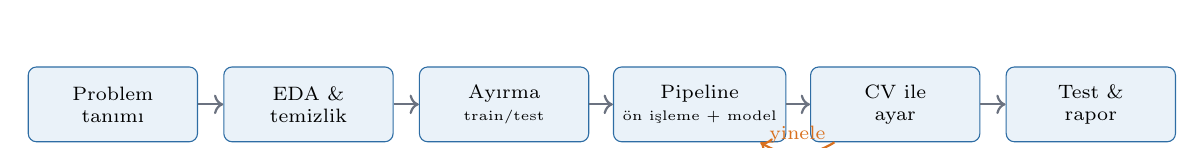
\begin{tikzpicture}[scale=0.92, every node/.style={font=\scriptsize},
  kutu/.style={draw=vurguMavi,fill=acikMavi,rounded corners=3pt,
               minimum width=2.15cm,minimum height=0.95cm,align=center}]
\node[kutu] (a) at (0,0) {Problem\\tanımı};
\node[kutu] (b) at (2.7,0) {EDA \&\\temizlik};
\node[kutu] (c) at (5.4,0) {Ayırma\\ \tiny train/test};
\node[kutu] (d) at (8.1,0) {Pipeline\\ \tiny ön işleme + model};
\node[kutu] (e) at (10.8,0) {CV ile\\ayar};
\node[kutu] (f) at (13.5,0) {Test \&\\rapor};
\foreach \x/\y in {a/b, b/c, c/d, d/e, e/f} \draw[->,thick,ortaGri] (\x)--(\y);
\draw[->,thick,turuncu] (e) to[bend left=32] node[above,turuncu]{yinele} (d);
\end{tikzpicture}
\end{center}

% =====================================================================
\gsec{Eğitim/Test Ayrımı ve Çapraz Doğrulama}
% =====================================================================

\uyari{\textbf{Altın kural:} test seti, model geliştirme sürecinin
\emph{hiçbir} adımında kullanılmaz --- ölçekleme parametrelerini, öznitelik
seçimini, hiperparametreleri, hatta ``hangi modeli deneyeyim'' kararını bile
etkilemez. Test setine bakarak alınan her karar, o setin tarafsızlığını yok
eder.}

\begin{lstlisting}
import numpy as np, pandas as pd
from sklearn.datasets import load_breast_cancer
from sklearn.model_selection import train_test_split, StratifiedKFold, cross_validate
from sklearn.pipeline import make_pipeline
from sklearn.preprocessing import StandardScaler
from sklearn.linear_model import LogisticRegression

bc = load_breast_cancer(as_frame=True)
X, y = bc.data, bc.target
print(bc.data.shape, np.bincount(y), bc.target_names)      # (569, 30) [212 357]

Xtr, Xte, ytr, yte = train_test_split(
    X, y, test_size=0.25, random_state=42, stratify=y)     # stratify: sinif orani korunur
print(f"pozitif oran: egitim={ytr.mean():.3f}  test={yte.mean():.3f}")
\end{lstlisting}

\begin{lstlisting}[style=outstyle]
(569, 30) [212 357] ['malignant' 'benign']
pozitif oran: egitim=0.627  test=0.629
\end{lstlisting}

\begin{lstlisting}
lr_ham  = LogisticRegression(max_iter=5000, random_state=42).fit(Xtr, ytr)
pipe    = make_pipeline(StandardScaler(),
                        LogisticRegression(max_iter=5000, random_state=42)).fit(Xtr, ytr)
print(f"olceklemesiz test dogrulugu = {lr_ham.score(Xte, yte):.4f}")
print(f"olcekli      test dogrulugu = {pipe.score(Xte, yte):.4f}")
\end{lstlisting}

\begin{lstlisting}[style=outstyle]
olceklemesiz test dogrulugu = 0.9580
olcekli      test dogrulugu = 0.9860
\end{lstlisting}

\bilgi{Sadece ölçekleme ekleyerek doğruluk \%95,8'den \%98,6'ya çıktı.
Mesafe ve gradyan temelli her yöntem (lojistik regresyon, SVM, $k$-NN, sinir
ağları, PCA) ölçeklemeye \emph{muhtaçtır}. Ağaç temelli yöntemler
(karar ağacı, Random Forest, Gradient Boosting) ise ölçeklemeden
etkilenmez.}

\gsub{Çapraz Doğrulama}

\nicin{\textbf{Tek bir eğitim/test ayrımı niçin yetmiyor?} Çünkü sonucun,
hangi \%20'nin teste düştüğüne bağlıdır. \code{random\_state} değerini
değiştirdiğinde doğruluğun \%94'ten \%97'ye zıplayabilir. Hangisi gerçek?
İkisi de değil --- ikisi de tek bir örneklemin gürültüsü.

\textbf{Çapraz doğrulama ne yapıyor?} Veriyi $k$ eşit parçaya böler.
Sırayla her parçayı test, kalan $k-1$ parçayı eğitim olarak kullanır. Sonunda
$k$ skorun ortalamasını alır. Böylece \emph{her gözlem tam bir kez} test
edilmiş olur --- ve elde ettiğin skor, tek bir şanslı/şanssız bölmeye değil,
verinin tamamına dayanır.

Bu, doğrudan Kısım 5'teki fikrin uygulamasıdır: tek bir tahmin yerine
\emph{tahminin dağılımına} bakarsın. $k$ skorun standart sapması, model
performansının belirsizliğini verir --- ve bu sayıyı raporlamak, ortalamayı
raporlamak kadar önemlidir. ``\%97,4 $\pm$ 1,7'' cümlesi, ``\%97,4''
cümlesinden çok daha dürüsttür.

\textbf{$k$ kaç olmalı?} 5 veya 10 standarttır. Küçük $k$: hızlı ama eğitim
kümesi küçüldüğü için skorlar biraz karamsar çıkar. Büyük $k$: daha doğru ama
$k$ kat pahalı. $n$ çok küçükse ($<50$) LeaveOneOut ($k=n$) kullanılır.

\textbf{Doğru stratejiyi seçmek --- en kritik karar.} Yandaki tablo bir
kontrol listesidir:
\begin{itemize}\itemsep1pt
\item \textbf{Sınıflandırma yapıyorsan} her zaman \code{StratifiedKFold}.
Sıradan \code{KFold}, dengesiz veride bir katmanda hiç pozitif örnek
bırakmayabilir.
\item \textbf{Aynı birimden birden çok satır varsa} (aynı hasta, aynı
kullanıcı, aynı mağaza) mutlaka \code{GroupKFold}. Aksi hâlde aynı hastanın
bir kaydı eğitimde, diğeri testte olur --- model hastayı tanır, hastalığı
değil. Bu, veri sızıntısının en sinsi biçimidir.
\item \textbf{Zaman boyutu varsa} \code{TimeSeriesSplit}. Rastgele bölmek,
modelin geleceği görmesine izin verir; ölçtüğün skor gerçek hayatta asla
tekrarlanmaz.
\end{itemize}

\textbf{Nerede kullanılır?} Model karşılaştırma; hiperparametre arama
(\code{GridSearchCV} içeride bunu çalıştırır); öznitelik seçiminin faydasını
ölçme; ve en önemlisi --- bir modelin üretime çıkmadan önceki tek dürüst
performans tahmini.}

\begin{center}
\begin{tabularx}{\textwidth}{@{}>{\ttfamily\color{anaMavi}}l >{\raggedright\arraybackslash}X@{}}
\toprule
\rowcolor{acikMavi}\multicolumn{1}{@{}l}{\color{anaMavi}\textbf{Strateji}} & \multicolumn{1}{l@{}}{\color{anaMavi}\textbf{Ne zaman?}}\\
\midrule
KFold & Genel amaçlı regresyon.\\
\rowcolor{acikGri} StratifiedKFold & Sınıflandırma --- sınıf oranlarını korur (varsayılan yap).\\
GroupKFold & Aynı hasta/kullanıcı/mağaza birden çok satırdaysa.\\
\rowcolor{acikGri} TimeSeriesSplit & Zaman serisi --- geleceği görmeyi engeller.\\
RepeatedStratifiedKFold & Küçük veride kararlı kestirim.\\
\rowcolor{acikGri} LeaveOneOut & Çok küçük veri ($n<50$); pahalı ve yüksek varyanslı.\\
\bottomrule
\end{tabularx}
\end{center}

\begin{lstlisting}
cv = StratifiedKFold(5, shuffle=True, random_state=42)
res = cross_validate(pipe, X, y, cv=cv,
                     scoring=['accuracy','roc_auc','f1','precision','recall'])
for k in ['test_accuracy','test_roc_auc','test_f1','test_precision','test_recall']:
    print(f"{k:>16}: {res[k].mean():.4f}")
\end{lstlisting}

\begin{lstlisting}[style=outstyle]
   test_accuracy: 0.9737
    test_roc_auc: 0.9953
         test_f1: 0.9794
  test_precision: 0.9683
     test_recall: 0.9916
\end{lstlisting}

% =====================================================================
\gsec{Veri Sızıntısı: En Pahalı Hata}
% =====================================================================

\nicin[Sızıntı Nedir ve Niçin Bu Kadar Tehlikeli?]{\textbf{Veri sızıntısı},
modelin eğitim sırasında \emph{tahmin anında sahip olamayacağı} bir bilgiye
erişmesidir. Sonuç yıkıcıdır: model laboratuvarda muhteşem skorlar verir,
üretimde çöker. Ve fark etmesi zordur --- çünkü hiçbir hata mesajı almazsın,
aksine \emph{çok iyi} sonuçlar alırsın.

\textbf{En yaygın dört biçimi:}
\begin{enumerate}\itemsep2pt
\item \textbf{Ön işlemeyi bölmeden önce yapmak.} \code{StandardScaler}'ı tüm
veriye uygulayıp sonra bölersen, ölçekleyici test kümesinin ortalamasını ve
sapmasını görmüş olur. Aynı şey \code{SimpleImputer}, \code{PCA},
öznitelik seçimi ve hedef kodlama (target encoding) için de geçerlidir ---
sonuncusu en tehlikelisidir. \emph{Çözüm:} her şeyi \code{Pipeline} içine
koy; çapraz doğrulama her katmanda ön işlemeyi baştan uydurur.
\item \textbf{Geleceği kullanmak.} ``Müşteri ayrılacak mı?'' modelinde
\code{iptal\_tarihi} sütununu öznitelik olarak vermek. Model \%100 doğruluk
verir --- ve tamamen işe yaramazdır.
\item \textbf{Aynı birimin hem eğitimde hem testte olması.} Aynı hastanın
iki taraması, aynı kullanıcının iki oturumu. \code{GroupKFold} ile önlenir.
\item \textbf{Test kümesine bakarak karar vermek.} Test skoruna göre model
seçip aynı test skorunu raporlamak. Test kümesi \emph{bir kez} kullanılır;
ayar için ayrı bir doğrulama kümesi (ya da iç içe çapraz doğrulama) gerekir.
\end{enumerate}

\textbf{Teşhis işaretleri:} Skorların ``çok iyi'' olması (\%99,9 doğruluk ---
gerçek problemler nadiren bu kadar kolaydır); beklenmedik bir özniteliğin
öneminin çok yüksek çıkması; üretimde performansın çakılması. \textbf{Kural:
Sonuç gerçek olamayacak kadar iyiyse, gerçek değildir.}

\textbf{Neden ``en pahalı hata''?} Çünkü diğer hatalar (yanlış model, kötü
hiperparametre) seni yalnızca \emph{daha kötü} bir modele götürür ve bunu
ölçebilirsin. Sızıntı ise ölçüm aracının kendisini bozar --- performansı
doğru ölçemediğin için hatalı modeli üretime alırsın, ve maliyeti orada
öğrenirsin.}

\tanim{\textbf{Veri sızıntısı} (data leakage), eğitim sırasında modele
gerçek kullanımda erişemeyeceği bilginin sızmasıdır. Sonuç: harika
doğrulama skorları, felaket bir üretim performansı.}

\begin{lstlisting}
from sklearn.feature_selection import SelectKBest, f_classif
from sklearn.pipeline import Pipeline
from sklearn.model_selection import cross_val_score

# Etkiyi cok net gormek icin: TAMAMEN rastgele veri (gercek bilgi = SIFIR)
rng = np.random.default_rng(0)
Xr = rng.normal(size=(100, 5000))
yr = rng.integers(0, 2, 100)

# YANLIS: ozellik secimini TUM veride yap, sonra CV
sec = SelectKBest(f_classif, k=20).fit(Xr, yr)
X_sizinti = sec.transform(Xr)
print("sizintili CV =",
      f"{cross_val_score(LogisticRegression(max_iter=2000), X_sizinti, yr, cv=5).mean():.4f}")

# DOGRU: secim pipeline icinde, her katlamada yeniden
pipe_dogru = Pipeline([('sel', SelectKBest(f_classif, k=20)),
                       ('clf', LogisticRegression(max_iter=2000))])
print("dogru     CV =", f"{cross_val_score(pipe_dogru, Xr, yr, cv=5).mean():.4f}")
\end{lstlisting}

\begin{lstlisting}[style=outstyle]
sizintili CV = 0.8500
dogru     CV = 0.4800
\end{lstlisting}

\uyari{Veride \emph{hiçbir} gerçek sinyal yokken sızıntı \%85 doğruluk
üretiyor; doğru yöntem ise \%48 (yani yazı-tura) diyor. Bu, yayımlanmış pek
çok ``mucize model''in gerçek açıklamasıdır.}

\begin{center}
\begin{tabularx}{\textwidth}{@{}>{\bfseries\color{kirmizi}}l >{\raggedright\arraybackslash}X@{}}
\toprule
\rowcolor{acikMavi}\multicolumn{1}{@{}l}{\color{anaMavi}\textbf{Sızıntı türü}} & \multicolumn{1}{l@{}}{\color{anaMavi}\textbf{Nasıl önlenir?}}\\
\midrule
Ön işleme sızıntısı & Ölçekleme/doldurma/kodlamayı \code{Pipeline} içine koy.\\
\rowcolor{acikGri} Öznitelik seçimi sızıntısı & Seçimi de pipeline'a al; her katlamada yeniden yap.\\
Hedef sızıntısı & Hedefin sonucunu içeren sütunları at (örn.\ ``iptal tarihi'' ile ``iptal etti mi'').\\
\rowcolor{acikGri} Zamansal sızıntı & Zaman serisinde \code{TimeSeriesSplit}; geleceği kullanma.\\
Grup sızıntısı & Aynı kişi hem eğitimde hem testte olmasın $\to$ \code{GroupKFold}.\\
\rowcolor{acikGri} Yinelenen satırlar & Ayırmadan önce \code{drop\_duplicates()}.\\
\bottomrule
\end{tabularx}
\end{center}

% =====================================================================
\gsec{Yanlılık--Varyans Dengesi}
% =====================================================================

\form[Hata Ayrıştırması]{
\[
\E\big[(y-\hat{f}(x))^2\big]
=\underbrace{\big(\E[\hat{f}(x)]-f(x)\big)^2}_{\text{yanlılık}^2}
+\underbrace{\Var(\hat{f}(x))}_{\text{varyans}}
+\underbrace{\sigma^2}_{\text{indirgenemez}}
\]
Basit modeller yüksek yanlılık (eksik öğrenme), karmaşık modeller yüksek
varyans (aşırı öğrenme) gösterir.}

\nicin{\textbf{Bu denklem makine öğrenmesinin en önemli tek denklemidir.}
Model hatanın nereden geldiğini üçe ayırır ve her biri farklı bir tedavi
gerektirir:

\begin{itemize}\itemsep2pt
\item \textbf{Yanlılık (bias)} --- modelin \emph{yanlış varsayımı}. Gerçek
ilişki eğriyken düz doğru uydurmak gibi. Ne kadar veri verirsen ver
düzelmez, çünkü sorun veride değil modelin kendisindedir. Belirtisi:
\emph{hem} eğitim \emph{hem} test hatası yüksek --- \textbf{eksik öğrenme}
(underfitting).
\item \textbf{Varyans} --- modelin \emph{aşırı hassasiyeti}. Eğitim
verisindeki gürültüyü de ezberler; birkaç örneği değiştirsen model tamamen
başkalaşır. Belirtisi: eğitim hatası çok düşük, test hatası yüksek ---
\textbf{aşırı öğrenme} (overfitting).
\item \textbf{İndirgenemez hata ($\sigma^2$)} --- verinin kendi gürültüsü.
Aynı özniteliklere sahip iki ev farklı fiyata satılır. Bu, hiçbir modelin
aşamayacağı tabandır. Bunu bilmek önemlidir: ``\%3 hataya inelim'' hedefi,
taban \%5 ise imkânsız bir hedeftir.
\end{itemize}

\textbf{Niçin ``denge''?} Çünkü ikisini aynı anda küçültemezsin. Modeli
karmaşıklaştırdıkça yanlılık düşer ama varyans yükselir. Toplam hata bu
yüzden U şeklinde bir eğri çizer --- en iyi model, en karmaşık model değil,
bu eğrinin dibindeki modeldir.

\textbf{Teşhis çok basit:} Eğitim ve test skorlarını karşılaştır.
\begin{itemize}\itemsep1pt
\item Eğitim \%70, test \%68 $\to$ yüksek yanlılık. \emph{Çözüm:} daha
karmaşık model, daha çok öznitelik, daha az düzenlileştirme. Daha çok veri
\emph{işe yaramaz}.
\item Eğitim \%99, test \%72 $\to$ yüksek varyans. \emph{Çözüm:} daha çok
veri, düzenlileştirme (Ridge/Lasso, dropout), daha basit model, topluluk
yöntemleri.
\end{itemize}
Bu tek karşılaştırma, ``modelim niçin kötü ve ne yapmalıyım?'' sorusunun
pratikteki en hızlı cevabıdır.

\textbf{Nerede karşına çıkar?} Aslında her yerde --- ve daha önce de çıktı:
Kısım 5'teki Bessel düzeltmesi tartışması (yanlı ama düşük varyanslı tahmin
edici), Ridge regresyonunun kasıtlı olarak yanlılık ekleyip varyans düşürmesi,
rastgele ormanın çok sayıda yüksek varyanslı ağacı ortalayarak varyansı
düşürmesi, boosting'in zayıf (yüksek yanlılıklı) öğrenicileri birleştirerek
yanlılığı düşürmesi. Kısım 9'daki tüm algoritmalar, bu dengede farklı bir
noktada durur.}

\gercek[Sınava Çalışmanın İki Yanlış Yolu]{Denge kavramını sezmenin en
kolay yolu bir öğrenci benzetmesidir:
\begin{itemize}\itemsep1pt
\item \textbf{Yüksek yanlılık:} Öğrenci konuyu hiç çalışmamış, her soruya
``B'' işaretliyor. Deneme sınavında da gerçek sınavda da aynı düşük notu
alır --- tutarlı biçimde kötü.
\item \textbf{Yüksek varyans:} Öğrenci geçen yılın sorularını
\emph{cevaplarıyla birlikte ezberlemiş}. Deneme sınavında 100 alıyor. Ama
gerçek sınavda sorular biraz değişince çakılıyor --- çünkü konuyu değil, o
soruların cevaplarını öğrendi.
\item \textbf{Denge:} Öğrenci konuyu anlamış. Deneme sınavında 85, gerçek
sınavda 82 alıyor. En yüksek deneme notu onun değil, ama gerçek sınavdaki en
yüksek not onun.
\end{itemize}
\textbf{Eğitim skoru, deneme sınavı notudur --- ve hiç kimse deneme notuna
göre işe alınmaz.} Model seçerken bakılması gereken tek şey test (veya
çapraz doğrulama) skorudur.}

\begin{lstlisting}
from sklearn.preprocessing import PolynomialFeatures
from sklearn.linear_model import LinearRegression

rng = np.random.default_rng(0)
Xp = rng.uniform(-3, 3, (60, 1))
yp = 0.5*Xp[:,0]**2 - Xp[:,0] + 2 + rng.normal(0, 1.2, 60)   # gercek: 2. derece
Xtr2, Xte2, ytr2, yte2 = train_test_split(Xp, yp, test_size=0.35, random_state=0)

print("derece | egitim MSE | test MSE")
for d in [1, 2, 3, 5, 9, 15]:
    m = make_pipeline(PolynomialFeatures(d), LinearRegression()).fit(Xtr2, ytr2)
    tr = np.mean((m.predict(Xtr2) - ytr2)**2)
    te = np.mean((m.predict(Xte2) - yte2)**2)
    print(f"{d:>6} | {tr:10.3f} | {te:8.3f}")
\end{lstlisting}

\begin{lstlisting}[style=outstyle]
derece | egitim MSE | test MSE
     1 |      2.211 |    4.003
     2 |      1.382 |    1.825
     3 |      1.373 |    1.816
     5 |      1.174 |    1.689
     9 |      0.842 |    2.748
    15 |      1.241 |    7.890
\end{lstlisting}

\begin{center}
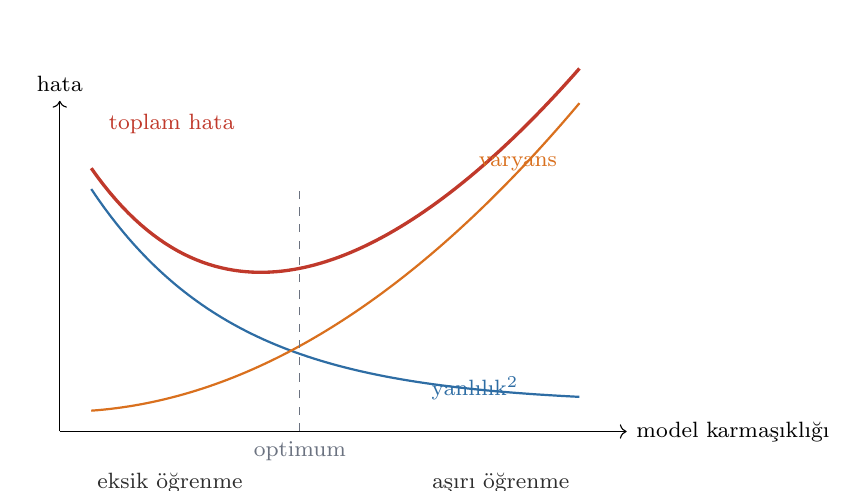
\begin{tikzpicture}[scale=1.0]
\draw[->] (0,0)--(7.2,0) node[right]{\footnotesize model karmaşıklığı};
\draw[->] (0,0)--(0,4.2) node[above]{\footnotesize hata};
\draw[grafikMavi,thick,domain=0.4:6.6,samples=80] plot (\x,{3.4*exp(-0.55*\x)+0.35});
\draw[turuncu,thick,domain=0.4:6.6,samples=80] plot (\x,{0.09*\x*\x+0.25});
\draw[kirmizi,very thick,domain=0.4:6.6,samples=80]
  plot (\x,{3.4*exp(-0.55*\x)+0.35+0.09*\x*\x+0.25});
\draw[dashed,ortaGri] (3.05,0)--(3.05,3.05);
\node[grafikMavi,right] at (4.6,0.55) {\footnotesize yanlılık$^2$};
\node[turuncu,right] at (5.2,3.4) {\footnotesize varyans};
\node[kirmizi,right] at (0.5,3.9) {\footnotesize toplam hata};
\node[ortaGri,below] at (3.05,0) {\footnotesize optimum};
\node[koyuGri] at (1.4,-0.65) {\footnotesize eksik öğrenme};
\node[koyuGri] at (5.6,-0.65) {\footnotesize aşırı öğrenme};
\end{tikzpicture}
\end{center}
\vspace{0.5cm}

\bilgi{Tablo eğrinin sayısal karşılığı: derece 1'de \emph{eksik öğrenme}
(hem eğitim hem test hatası yüksek), derece 3--5'te optimum, derece 15'te
\emph{aşırı öğrenme} (eğitim hatası düşük, test hatası $7{,}89$'a fırlıyor).
Eğitim ile test hatası arasındaki \emph{makas}, aşırı öğrenmenin
göstergesidir.}

\gsub{Öğrenme Eğrileri: Daha Fazla Veri İşe Yarar mı?}

\begin{lstlisting}
from sklearn.model_selection import learning_curve
import matplotlib.pyplot as plt

boyut, tr_sk, te_sk = learning_curve(
    pipe, X, y, cv=cv, train_sizes=np.linspace(0.1, 1.0, 8),
    scoring='accuracy', n_jobs=-1)

plt.plot(boyut, tr_sk.mean(1), 'o-', label='egitim')
plt.plot(boyut, te_sk.mean(1), 's-', label='dogrulama')
plt.fill_between(boyut, te_sk.mean(1)-te_sk.std(1), te_sk.mean(1)+te_sk.std(1), alpha=.2)
plt.xlabel('egitim ornegi sayisi'); plt.ylabel('dogruluk'); plt.legend(); plt.show()
\end{lstlisting}

\ipucu{Öğrenme eğrisi okuma: (1) İki eğri de düşük ve birleşmişse
\emph{yüksek yanlılık} $\to$ daha karmaşık model, daha iyi öznitelik.
(2) Arada büyük makas varsa \emph{yüksek varyans} $\to$ daha çok veri,
düzenlileştirme, daha basit model. (3) Doğrulama eğrisi düzleşmişse
\textbf{daha fazla veri toplamak para kaybıdır}.}

% =====================================================================
\gsec{Ön İşleme ve Pipeline}
% =====================================================================

\begin{lstlisting}
from sklearn.compose import ColumnTransformer
from sklearn.impute import SimpleImputer
from sklearn.preprocessing import OneHotEncoder, StandardScaler
from sklearn.pipeline import Pipeline
import seaborn as sns

tit = sns.load_dataset('titanic')
sayisal   = ['age', 'fare', 'sibsp', 'parch']
kategorik = ['sex', 'embarked', 'class', 'who', 'alone']

on_isleme = ColumnTransformer([
    ('num', Pipeline([('imp', SimpleImputer(strategy='median')),
                      ('sc',  StandardScaler())]), sayisal),
    ('cat', Pipeline([('imp', SimpleImputer(strategy='most_frequent')),
                      ('oh',  OneHotEncoder(handle_unknown='ignore',
                                            drop='first'))]), kategorik),
])

model = Pipeline([('prep', on_isleme),
                  ('clf', LogisticRegression(max_iter=2000, random_state=42))])
\end{lstlisting}

\begin{center}
\begin{tabularx}{\textwidth}{@{}>{\ttfamily\color{anaMavi}}l >{\raggedright\arraybackslash}X@{}}
\toprule
\rowcolor{acikMavi}\multicolumn{1}{@{}l}{\color{anaMavi}\textbf{Dönüştürücü}} & \multicolumn{1}{l@{}}{\color{anaMavi}\textbf{Ne yapar / ne zaman?}}\\
\midrule
StandardScaler & $(x-\mu)/\sigma$. Varsayılan tercih.\\
\rowcolor{acikGri} MinMaxScaler & $[0,1]$ aralığına sıkıştırır; sinir ağlarında yaygın.\\
RobustScaler & Medyan ve IQR kullanır; aykırı değer varsa.\\
\rowcolor{acikGri} PowerTransformer & Yeo-Johnson/Box-Cox; çarpıklığı giderir.\\
QuantileTransformer & Dağılımı normale/düzgüne zorlar.\\
\rowcolor{acikGri} OneHotEncoder & Kategorik $\to$ ikili sütunlar. \code{drop='first'} eşdoğrusallığı önler.\\
OrdinalEncoder & Sıralı kategoriler için (ağaç modellerinde de uygun).\\
\rowcolor{acikGri} TargetEncoder & Yüksek kardinaliteli kategoriler; sızıntıya dikkat.\\
SimpleImputer / KNNImputer & Eksik değer doldurma.\\
\rowcolor{acikGri} PolynomialFeatures & Etkileşim ve polinom terimleri.\\
\bottomrule
\end{tabularx}
\end{center}

% =====================================================================
\gsec{Değerlendirme Metrikleri}
% =====================================================================

\gsub{Sınıflandırma}

\nicin[Niçin Tek Bir Metrik Yetmiyor?]{``Modelim \%99 doğru'' cümlesi çoğu
zaman hiçbir şey ifade etmez. Bir hastalık toplumda binde bir görülüyorsa,
\emph{herkese ``sağlıklı'' diyen} bir model \%99,9 doğruluk alır --- ve tek
bir hastayı bile bulamaz. Doğruluk, sınıflar dengesizken tamamen yanıltıcıdır
(Kısım 3'teki taban oranı yanılgısının makine öğrenmesindeki karşılığı).

\textbf{Önce dört sayıyı tanı --- her metrik bunlardan türer:}
\begin{itemize}\itemsep1pt
\item \textbf{TP} (doğru pozitif): Hasta dedin, gerçekten hasta.
\item \textbf{TN} (doğru negatif): Sağlıklı dedin, gerçekten sağlıklı.
\item \textbf{FP} (yanlış pozitif): Hasta dedin, aslında sağlıklı ---
\emph{yanlış alarm}, Tip I hata.
\item \textbf{FN} (yanlış negatif): Sağlıklı dedin, aslında hasta ---
\emph{kaçırma}, Tip II hata.
\end{itemize}

\textbf{İki temel metrik, iki farklı soru:}
\begin{itemize}\itemsep2pt
\item \textbf{Kesinlik (precision)} $=TP/(TP+FP)$: \emph{``Pozitif dediklerimin
kaçı gerçekten pozitifti?''} Alarm verdiğinde ne kadar güvenilirsin.
\emph{Yanlış alarm pahalıysa} bunu optimize et --- spam filtresi (önemli
e-postayı silmek felaket), otomatik kredi reddi, hedefli pahalı pazarlama
kampanyası.
\item \textbf{Duyarlılık (recall)} $=TP/(TP+FN)$: \emph{``Gerçek pozitiflerin
kaçını yakaladım?''} Kaçırma oranın ne.
\emph{Kaçırmak pahalıysa} bunu optimize et --- kanser taraması, dolandırıcılık
tespiti, güvenlik kamerası, üretim hattında kusurlu parça tespiti.
\end{itemize}
İkisi \textbf{birbiriyle çelişir}: eşiği düşürünce daha çok pozitif dersin,
duyarlılık artar ama kesinlik düşer. Bu tam olarak Kısım 6'daki $\alpha$--$\beta$
dengesidir --- aynı matematik, farklı isimler.

\textbf{F1 niçin harmonik ortalama?} Kısım 2'de gördüğümüz gibi harmonik
ortalama küçük değere yapışır. Kesinlik $0{,}99$, duyarlılık $0{,}02$ olan bir
model F1 $=0{,}039$ alır --- ``bir tarafı berbatsa model berbattır''.
Aritmetik ortalama alsaydık $0{,}5$ çıkardı ve model iyi görünürdü.

\textbf{ROC-AUC ne ölçer?} Eşikten \emph{bağımsız} olarak, modelin rastgele
bir pozitifi rastgele bir negatiften daha yüksek puanlama olasılığı.
$0{,}5$ = madenî para atmak, $1{,}0$ = kusursuz sıralama. Model
karşılaştırmak için idealdir çünkü eşik seçimini denklemden çıkarır.

\textbf{Ne zaman PR-AUC?} Sınıflar ciddi biçimde dengesizse. ROC eğrisi,
çoğunluk sınıfı çok büyükse yanıltıcı biçimde iyi görünür (paydadaki TN
devasadır, FP oranını bastırır). PR eğrisi TN'yi hiç kullanmaz, bu yüzden
azınlık sınıfına odaklanır. \emph{Kural:} pozitif sınıf \%10'un altındaysa
PR-AUC raporla.

\textbf{Log loss niçin ayrı bir metrik?} Diğerleri yalnızca kararın doğru
olup olmadığına bakar; log loss \emph{ne kadar emin olduğuna} da bakar.
``\%51 ihtimalle hasta'' ile ``\%99 ihtimalle hasta'' aynı kararı verir ama
çok farklı bilgilerdir. Olasılığı bir sonraki adımda kullanacaksan (risk
fiyatlama, beklenen değer hesabı, eşik optimizasyonu) log loss ve
kalibrasyon (Kısım 11) kritik hâle gelir.}

\begin{center}
\begin{tabularx}{\textwidth}{@{}>{\bfseries\color{anaMavi}}l >{$\displaystyle}l<{$} >{\raggedright\arraybackslash}X@{}}
\toprule
\rowcolor{acikMavi}\multicolumn{1}{@{}l}{\color{anaMavi}\textbf{Metrik}} & \multicolumn{1}{l}{\color{anaMavi}\textbf{Formül}} & \multicolumn{1}{l@{}}{\color{anaMavi}\textbf{Ne zaman?}}\\
\midrule
Doğruluk & \frac{TP+TN}{N} & Dengeli sınıflar.\\
\rowcolor{acikGri} Kesinlik & \frac{TP}{TP+FP} & Yanlış alarmın maliyeti yüksekse.\\
Duyarlılık & \frac{TP}{TP+FN} & Kaçırmanın maliyeti yüksekse (tıp!).\\
\rowcolor{acikGri} F1 & \frac{2PR}{P+R} & Kesinlik--duyarlılık dengesi.\\
ROC-AUC & \text{eğri altı alan} & Eşikten bağımsız sıralama kalitesi.\\
\rowcolor{acikGri} PR-AUC & \text{eğri altı alan} & \textbf{Dengesiz} veride ROC'tan iyi.\\
Log loss & -\frac1N\sum[y\log\hat p+(1-y)\log(1-\hat p)] & Olasılık kalitesi (kalibrasyon).\\
\bottomrule
\end{tabularx}
\end{center}

\begin{lstlisting}
from sklearn.metrics import (confusion_matrix, classification_report,
                             roc_auc_score, average_precision_score, log_loss)

yhat  = pipe.predict(Xte)
yprob = pipe.predict_proba(Xte)[:, 1]

cm = confusion_matrix(yte, yhat)
tn, fp, fn, tp = cm.ravel()
print(f"TN={tn}  FP={fp}  FN={fn}  TP={tp}")
print(f"roc_auc  = {roc_auc_score(yte, yprob):.4f}")
print(f"pr_auc   = {average_precision_score(yte, yprob):.4f}")
print(f"log_loss = {log_loss(yte, yprob):.4f}")
print(classification_report(yte, yhat, target_names=bc.target_names))
\end{lstlisting}

\begin{lstlisting}[style=outstyle]
TN=52  FP=1  FN=1  TP=89
roc_auc  = 0.9977
pr_auc   = 0.9986
log_loss = 0.0679
              precision    recall  f1-score   support

   malignant       0.98      0.98      0.98        53
      benign       0.99      0.99      0.99        90

    accuracy                           0.99       143
   macro avg       0.99      0.99      0.99       143
weighted avg       0.99      0.99      0.99       143
\end{lstlisting}

\uyari{Bu problemde \code{malignant} (kötü huylu) sınıfı için \textbf{1 yanlış
negatif} var: bir kanser vakası kaçırıldı. Tıbbi tanıda bu, yanlış alarmdan
çok daha pahalıdır. Doğru yaklaşım, karar eşiğini $0{,}5$'te bırakmak yerine
duyarlılığı artıracak biçimde düşürmektir (Kısım 11).}

\gsub{Regresyon}

\nicin[Hangi Hata Metriği, Niçin?]{Hepsi ``tahminim gerçekten ne kadar
uzak?'' sorusunu ölçer, ama \emph{hataları nasıl cezalandırdıkları} farklıdır
--- ve bu fark, modelinin neyi optimize edeceğini belirler.

\begin{itemize}\itemsep2pt
\item \textbf{MSE / RMSE --- büyük hatalar orantısız kötüdür.} Kare aldığı
için 10 birimlik bir hata, 1 birimlik on hatadan \emph{10 kat} daha ağır
sayılır. \emph{Ne zaman doğru:} Tek bir büyük hata felaketse --- ilaç dozu,
uçuş rotası, elektrik şebekesi yük tahmini, stok planlaması. Ayrıca
matematiksel olarak uysal olduğu için (türevlenebilir) neredeyse tüm modeller
varsayılan olarak MSE optimize eder.
\item \textbf{MAE --- her hata kendi büyüklüğü kadar kötüdür.} Aykırı
değerlerden etkilenmez. \emph{Ne zaman doğru:} Veride silemediğin uç
gözlemler varsa; ``ortalama olarak kaç TL yanılıyorum?'' sorusu iş için
anlamlıysa. Not: MSE'yi minimize eden tahmin \emph{ortalamadır}, MAE'yi
minimize eden \emph{medyandır} --- yani metrik seçimi, modelin neyi tahmin
ettiğini değiştirir.
\item \textbf{RMSE mi MAE mi?} RMSE her zaman MAE'den büyük veya eşittir;
aradaki fark ne kadar açıksa, hata dağılımında o kadar çok uç değer var
demektir. İkisini birlikte raporlamak bu yüzden bilgilendiricidir.
\item \textbf{$R^2$ --- ``modelim hiçbir şey bilmemekten ne kadar iyi?''}
Payda, her zaman ortalamayı tahmin eden aptal modelin hatasıdır. $R^2=0{,}76$
demek ``o aptal modele göre hatanın \%76'sını yok ettim'' demektir. $R^2$
negatif de olabilir --- modelin ortalamadan kötüyse. Birimsiz olduğu için
farklı problemler arasında karşılaştırılabilir; ama \emph{aynı} problemde
model seçerken RMSE daha somuttur.
\item \textbf{MAPE --- yüzde cinsinden hata.} İş birimlerine anlatması en
kolay metriktir (``\%8 sapmayla tahmin ediyoruz''). \emph{Tuzağı:} $y$ sıfıra
yaklaşınca patlar, ve düşük tahminleri yüksek tahminlerden daha az
cezalandırır (asimetriktir). Sıfıra yakın değerler varsa MAPE yerine sMAPE
veya MAE kullan.
\end{itemize}

\textbf{Pratik kural:} Metriği modelden \emph{önce} seç ve iş sorusuna göre
seç. ``Hangi metrik daha iyi çıkıyorsa onu raporlarım'' yaklaşımı, sonuçları
kendi lehine seçmenin bir biçimidir.}

\gercek[Yanlış Metrik, Yanlış Model]{Bir e-ticaret şirketi günlük talep
tahmini yapıyor. Ürünlerin \%95'i günde 0--5 adet satıyor, \%5'i ise
kampanya günlerinde 500--1000 adet.

RMSE ile optimize edilen model, o \%5'lik kampanya gününü kaçırmamaya
odaklanır --- çünkü oradaki hatanın karesi devasadır. Sonuç: normal günlerde
sürekli fazla stok tahmini yapar, depo dolar.

MAE ile optimize edilen model ise \%95'lik çoğunluğa odaklanır, kampanya
günlerini kaçırır --- ve o günlerde stoksuz kalınır, asıl para orada kaybedilir.

Doğru çözüm metriği değiştirmek değil, \textbf{problemi bölmektir}: normal
günler ve kampanya günleri için ayrı modeller. Metrik tartışması çoğu zaman
gizli bir ``problem yanlış kurulmuş'' sinyalidir.}

\begin{center}
\begin{tabularx}{\textwidth}{@{}>{\bfseries\color{anaMavi}}l >{$\displaystyle}l<{$} >{\raggedright\arraybackslash}X@{}}
\toprule
\rowcolor{acikMavi}\multicolumn{1}{@{}l}{\color{anaMavi}\textbf{Metrik}} & \multicolumn{1}{l}{\color{anaMavi}\textbf{Formül}} & \multicolumn{1}{l@{}}{\color{anaMavi}\textbf{Özellik}}\\
\midrule
MSE & \tfrac1n\sum(y-\hat y)^2 & Büyük hataları çok cezalandırır.\\
\rowcolor{acikGri} RMSE & \sqrt{\text{MSE}} & $y$ ile aynı birim.\\
MAE & \tfrac1n\sum|y-\hat y| & Aykırı değere dayanıklı.\\
\rowcolor{acikGri} $R^2$ & 1-\tfrac{\text{SS}_{res}}{\text{SS}_{tot}} & Açıklanan varyans oranı.\\
MAPE & \tfrac1n\sum\left|\tfrac{y-\hat y}{y}\right| & Yüzde hata; $y\approx0$'da patlar.\\
\bottomrule
\end{tabularx}
\end{center}

\uyari{scikit-learn'de skorlar \emph{büyük daha iyi} kuralına uyar; bu yüzden
\code{scoring='neg\_mean\_squared\_error'} gibi negatif isimler görürsün.
\code{cross\_val\_score} çıktısının işaretini çevirmeyi unutma.}

% #####################################################################
\gpart{9}{Denetimli Öğrenme Algoritmaları}
% #####################################################################

% =====================================================================
\gsec{Algoritma Haritası}
% =====================================================================

\begin{center}
\begin{tabularx}{\textwidth}{@{}>{\bfseries\color{anaMavi}}l >{\raggedright\arraybackslash}X >{\raggedright\arraybackslash}X@{}}
\toprule
\rowcolor{acikMavi}\multicolumn{1}{@{}l}{\color{anaMavi}\textbf{Algoritma}} & \multicolumn{1}{l}{\color{anaMavi}\textbf{Güçlü yanı}} & \multicolumn{1}{l@{}}{\color{anaMavi}\textbf{Zayıf yanı}}\\
\midrule
Lojistik regresyon & Yorumlanabilir, hızlı, kalibre olasılık & Yalnız doğrusal sınır\\
\rowcolor{acikGri} $k$-NN & Varsayımsız, basit & Yavaş tahmin, boyut laneti, ölçekleme şart\\
Naive Bayes & Çok hızlı, az veriyle çalışır & Bağımsızlık varsayımı gerçekçi değil\\
\rowcolor{acikGri} SVM & Yüksek boyutta güçlü, kernel esnekliği & Büyük veride yavaş, olasılık vermez\\
Karar ağacı & Yorumlanabilir, ölçekleme gerekmez & Kararsız, kolay aşırı öğrenir\\
\rowcolor{acikGri} Random Forest & Sağlam, ayar gerektirmez & Yorumlanması zor, büyük bellek\\
Gradient Boosting & Genelde en yüksek doğruluk & Ayar hassas, aşırı öğrenebilir\\
\rowcolor{acikGri} Sinir ağı & Karmaşık örüntüler & Çok veri ister, kara kutu\\
\bottomrule
\end{tabularx}
\end{center}

\gsub{Hepsini Aynı Veride Karşılaştırmak}

\begin{lstlisting}
import numpy as np, pandas as pd, time
from sklearn.datasets import load_breast_cancer
from sklearn.model_selection import cross_val_score, StratifiedKFold
from sklearn.pipeline import make_pipeline
from sklearn.preprocessing import StandardScaler
from sklearn.linear_model import LogisticRegression
from sklearn.neighbors import KNeighborsClassifier
from sklearn.naive_bayes import GaussianNB
from sklearn.svm import SVC
from sklearn.tree import DecisionTreeClassifier
from sklearn.ensemble import (RandomForestClassifier, ExtraTreesClassifier,
                              AdaBoostClassifier, GradientBoostingClassifier,
                              HistGradientBoostingClassifier)

bc = load_breast_cancer(as_frame=True); X, y = bc.data, bc.target
cv = StratifiedKFold(5, shuffle=True, random_state=42)

modeller = {
 'LogisticRegression':   make_pipeline(StandardScaler(), LogisticRegression(max_iter=5000, random_state=42)),
 'kNN (k=5)':            make_pipeline(StandardScaler(), KNeighborsClassifier(5)),
 'GaussianNB':           make_pipeline(StandardScaler(), GaussianNB()),
 'SVM (rbf)':            make_pipeline(StandardScaler(), SVC(random_state=42)),
 'DecisionTree':         DecisionTreeClassifier(random_state=42),
 'RandomForest':         RandomForestClassifier(n_estimators=300, random_state=42, n_jobs=-1),
 'ExtraTrees':           ExtraTreesClassifier(n_estimators=300, random_state=42, n_jobs=-1),
 'AdaBoost':             AdaBoostClassifier(random_state=42),
 'GradientBoosting':     GradientBoostingClassifier(random_state=42),
 'HistGradientBoosting': HistGradientBoostingClassifier(random_state=42),
}

satirlar = []
for ad, m in modeller.items():
    t0 = time.perf_counter()
    acc = cross_val_score(m, X, y, cv=cv, scoring='accuracy', n_jobs=-1)
    auc = cross_val_score(m, X, y, cv=cv, scoring='roc_auc',  n_jobs=-1)
    satirlar.append({'model': ad, 'accuracy': acc.mean(), 'std': acc.std(),
                     'roc_auc': auc.mean(), 'sure_s': time.perf_counter()-t0})

print(pd.DataFrame(satirlar).sort_values('roc_auc', ascending=False).round(4))
\end{lstlisting}

\begin{lstlisting}[style=outstyle]
               model  accuracy    std  roc_auc  sure_s
  LogisticRegression    0.9737 0.0166   0.9953  1.4124
           SVM (rbf)    0.9772 0.0163   0.9945  0.0460
          ExtraTrees    0.9649 0.0157   0.9941  0.4697
            AdaBoost    0.9525 0.0219   0.9933  0.2171
    GradientBoosting    0.9491 0.0237   0.9927  0.4894
HistGradientBoosting    0.9666 0.0129   0.9925  0.2062
        RandomForest    0.9526 0.0131   0.9895  0.6589
          GaussianNB    0.9297 0.0199   0.9860  0.0452
           kNN (k=5)    0.9631 0.0179   0.9849  1.0836
        DecisionTree    0.9104 0.0279   0.9000  0.0651
\end{lstlisting}

\bilgi{Sürpriz: en basit model olan \textbf{lojistik regresyon} en yüksek
ROC-AUC'yi veriyor. Bu veri seti doğrusal olarak ayrılabilir olduğu için
karmaşık modeller ek değer katmıyor. \textbf{Ders:} her zaman basit bir
temel çizgi (baseline) kur; gradient boosting'e atlamadan önce onu yenmen
gerektiğini bil.}

% =====================================================================
\gsec{$k$-En Yakın Komşu}
% =====================================================================

\form{Tahmin, en yakın $k$ komşunun oyu (sınıflandırma) ya da ortalamasıdır
(regresyon). Eğitim yoktur --- \emph{tembel öğrenme}. Uzaklık genelde
Öklid'dir:
$d(x,x')=\sqrt{\sum_j (x_j-x'_j)^2}$.}

\nicin{\textbf{Fikir tek cümlede:} ``Bana benzeyenlere bak, onların cevabını
ver.'' Yeni bir gözlem geldiğinde, eğitim verisindeki en yakın $k$ komşuyu
bulur ve onların çoğunluk sınıfını (ya da ortalamasını) döndürür. Hiçbir
denklem uydurmaz, hiçbir parametre öğrenmez --- bu yüzden \emph{tembel
öğrenme} denir: bütün işi tahmin anına erteler.

\textbf{Niçin öğrenmesi gerekmiyor?} Çünkü modeli, verinin kendisidir.
Eğitim aşaması sadece veriyi hafızaya almaktır (O(1)); asıl maliyet tahmin
anında ortaya çıkar, çünkü her yeni nokta için tüm eğitim kümesine uzaklık
hesaplanır. Bu, diğer algoritmaların tam tersidir --- ve $k$-NN'in milyonlarca
satırlık veride niçin kullanılmadığını açıklar.

\textbf{$k$ neyi kontrol eder?} Doğrudan yanlılık--varyans düğmesidir.
$k=1$: karar sınırı her gözleme uyar, gürültüyü ezberler (yüksek varyans).
$k$ çok büyük: her şey ortalanır, ince yapı kaybolur (yüksek yanlılık).
Tabloda $k=3$ optimum çıkıyor. Pratik başlangıç: $k\approx\sqrt{n}$, ve
sınıflandırmada beraberliği önlemek için tek sayı seç.

\textbf{Ölçekleme niçin \emph{zorunlu}?} Uzaklık hesabı birimlere duyarlıdır.
``Maaş'' (30.000--90.000) ve ``yaş'' (20--65) özniteliklerini birlikte
kullanırsan, maaştaki 1000 TL'lik fark yaştaki 45 yıllık farktan büyük görünür
--- yaş fiilen yok sayılır. \code{StandardScaler} olmadan $k$-NN neredeyse her
zaman yanlıştır.

\textbf{Boyut laneti niçin $k$-NN'i özellikle vurur?} Yüksek boyutta tüm
noktalar birbirine yaklaşık eşit uzaklıkta olur; ``en yakın komşu'' kavramı
anlamını yitirir. 100 boyutta $k$-NN genellikle rastgeleden az iyidir.
Çözüm: önce PCA ile boyut indirgemek veya öznitelik seçimi yapmak.

\textbf{Nerede kullanılır?}
\begin{itemize}\itemsep1pt
\item \textbf{Öneri sistemleri:} ``Senin gibi kullanıcılar şunu beğendi'' ---
işbirlikçi filtrelemenin en basit hâli birebir $k$-NN'dir.
\item \textbf{Görüntü/yüz eşleştirme:} Gömme vektörleri (embedding)
çıkarıldıktan sonra en yakın komşu araması. Modern vektör veritabanları
(FAISS, pgvector) endüstriyel ölçekte $k$-NN motorlarıdır.
\item \textbf{Eksik veri doldurma:} \code{KNNImputer}, eksik değeri benzer
satırların ortalamasıyla doldurur.
\item \textbf{Hızlı temel model (baseline):} Yeni bir problemde ``bu veri
öğrenilebilir mi?'' sorusunun en hızlı testi.
\end{itemize}}

\begin{lstlisting}
for k in [1, 3, 5, 11, 21, 51]:
    s = cross_val_score(make_pipeline(StandardScaler(), KNeighborsClassifier(k)),
                        X, y, cv=cv)
    print(f"k = {k:>3}: {s.mean():.4f}")
\end{lstlisting}

\begin{lstlisting}[style=outstyle]
k =   1: 0.9508
k =   3: 0.9666
k =   5: 0.9631
k =  11: 0.9631
k =  21: 0.9526
k =  51: 0.9490
\end{lstlisting}

\uyari{$k=1$ eğitim verisini ezberler (aşırı öğrenme), $k$ çok büyükse her
şeyi ortalar (eksik öğrenme). $k$ tam olarak \emph{yanlılık--varyans}
düğmesidir. Ayrıca $k$-NN ölçeklemesiz kullanılamaz: birimi büyük olan
öznitelik uzaklığı domine eder. \textbf{Boyut laneti}: özellik sayısı
arttıkça tüm noktalar birbirine eşit uzaklıkta görünmeye başlar.}

% =====================================================================
\gsec{Karar Ağaçları}
% =====================================================================

\form[Bölme Ölçütleri]{Bir düğümü, çocuk düğümlerin \emph{saflığını} en çok
artıran özellik--eşik çiftiyle böl:
\[
\text{Gini}=1-\sum_c p_c^2,
\qquad
\text{Entropi}=-\sum_c p_c\log_2 p_c,
\qquad
\text{Regresyonda: MSE azalması}.
\]}

\nicin{\textbf{Ağaç ne yapıyor?} Veriyi ardışık evet/hayır sorularıyla giderek
daha \emph{saf} parçalara böler. ``Saf'' demek, bir yaprakta çoğunlukla tek
bir sınıfın kalması demektir. Aşağıdaki çıktıda iki soru --- ``en kötü yarıçap
16,8'den küçük mü?'' ve ``içbükey nokta sayısı 0,14'ten küçük mü?'' --- \%90
doğruluk veriyor.

\textbf{Gini ve entropi ne ölçüyor?} İkisi de \emph{safsızlığı} ölçer.
Bir düğümde tek sınıf varsa ikisi de 0; sınıflar yarı yarıyaysa ikisi de en
büyük değerini alır (Gini $0{,}5$, entropi 1). Ağaç her adımda tüm olası
bölmeleri dener ve safsızlığı en çok düşüreni seçer --- buna \emph{bilgi
kazancı} denir.

\textbf{Gini mi entropi mi?} Pratikte neredeyse hiç fark etmezler; aynı
ağaçları üretirler. Gini biraz daha hızlıdır (logaritma yok), bu yüzden
varsayılan odur. Entropi bilgi kuramından gelir ve ``bu bölme kaç bit belirsizlik
azalttı?'' diye okunabilir.

\textbf{Regresyonda MSE azalması --- tanıdık geldi mi?} Bu, Kısım 3'teki
\emph{varyans ayrıştırmasının} ta kendisidir: ağaç, gruplar arası varyansı
en çok büyüten bölmeyi arar. ANOVA, $R^2$ ve karar ağacı bölmesi aynı fikrin
üç yüzüdür.

\textbf{Ağaçların ayırt edici üstünlükleri:}
\begin{itemize}\itemsep1pt
\item \textbf{Yorumlanabilirlik:} Sonucu bir akış şeması olarak çizip
alan uzmanıyla tartışabilirsin. Hiçbir başka model bunu bu kadar doğrudan
yapamaz.
\item \textbf{Ölçekleme gerektirmez:} Eşik karşılaştırması yaptığı için
birimler önemsizdir.
\item \textbf{Doğrusal olmayan ilişkileri ve etkileşimleri kendiliğinden
yakalar:} ``Eğer erkekse \emph{ve} 3.\ sınıftaysa'' kuralı, regresyonda
elle eklemen gereken bir etkileşim terimidir.
\item \textbf{Karma veri tipleriyle çalışır:} Kategorik ve sayısal
öznitelikler bir arada.
\end{itemize}

\textbf{En büyük zayıflığı: kararsızlık.} Veriden birkaç örneği değiştirsen
ağaç bambaşka çıkabilir --- yüksek varyanslı bir modeldir. Kısım 9'daki
topluluk yöntemleri (rastgele orman, gradyan artırma) tam olarak bu zayıflığı
kapatmak için icat edildi: yüzlerce oynak ağacın ortalaması, tek bir ağaçtan
çok daha kararlıdır.

\textbf{Nerede kullanılır?} Kredi onay kuralları; tıbbi triyaj protokolleri
(acil serviste hangi hasta önce görülecek); müşteri segmentasyonu kuralları;
sigortada risk sınıflandırması; ve en önemlisi --- gradyan artırma
kütüphanelerinin (XGBoost, LightGBM) yapı taşı olarak, tablo verisindeki
en güçlü modellerin temeli.}

\begin{lstlisting}
from sklearn.tree import DecisionTreeClassifier, export_text
for d in [1, 2, 3, 5, 10, None]:
    s = cross_val_score(DecisionTreeClassifier(max_depth=d, random_state=42), X, y, cv=cv)
    print(f"max_depth = {str(d):>4}: {s.mean():.4f}")

dt = DecisionTreeClassifier(max_depth=2, random_state=42).fit(X, y)
print(export_text(dt, feature_names=list(X.columns), max_depth=2))
\end{lstlisting}

\begin{lstlisting}[style=outstyle]
max_depth =    1: 0.8876
max_depth =    2: 0.9052
max_depth =    3: 0.9245
max_depth =    5: 0.9280
max_depth =   10: 0.9104
max_depth = None: 0.9104

|--- worst radius <= 16.80
|   |--- worst concave points <= 0.14
|   |   |--- class: 1
|   |--- worst concave points >  0.14
|   |   |--- class: 0
|--- worst radius >  16.80
|   |--- mean texture <= 16.11
|   |   |--- class: 1
|   |--- mean texture >  16.11
|   |   |--- class: 0
\end{lstlisting}

\bilgi{Sadece iki soruyla \%90 doğruluk: ``en kötü yarıçap 16,8'den küçük mü?''
ve ``en kötü içbükey nokta sayısı 0,14'ten küçük mü?'' Karar ağaçlarının
büyük değeri budur --- bir doktora gösterip tartışabileceğin kurallar üretir.
Derinlik arttıkça doğruluk düşüyor (aşırı öğrenme), bu yüzden
\code{max\_depth}, \code{min\_samples\_leaf}, \code{ccp\_alpha} ile budama
şarttır.}

% =====================================================================
\gsec{Destek Vektör Makineleri (SVM)}
% =====================================================================

\form[Maksimum Marj]{SVM, iki sınıfı ayıran hiperdüzlemler arasından
\emph{marjı} (sınıflara en yakın noktaların uzaklığını) en büyük olanı seçer:
\[
\min_{w,b}\ \tfrac12\|w\|^2 + C\sum_i \xi_i
\quad\text{öyle ki}\quad
y_i(w^\top x_i+b)\ge 1-\xi_i,\ \ \xi_i\ge0 .
\]
$C$, marj genişliği ile hata toleransı arasındaki dengeyi kurar: büyük $C$
$\to$ dar marj, az hata (aşırı öğrenme riski).}

\begin{center}
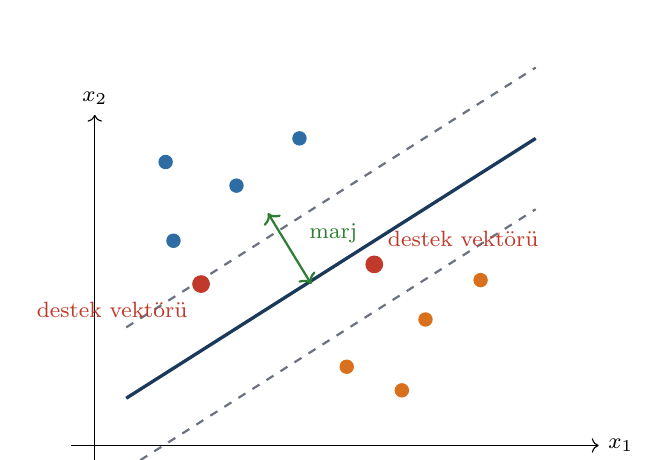
\begin{tikzpicture}[scale=1.0]
\draw[->] (-0.3,0)--(6.4,0) node[right]{\footnotesize $x_1$};
\draw[->] (0,-0.3)--(0,4.2) node[above]{\footnotesize $x_2$};
\draw[anaMavi,very thick] (0.4,0.6)--(5.6,3.9);
\draw[ortaGri,dashed,thick] (0.4,1.5)--(5.6,4.8);
\draw[ortaGri,dashed,thick] (0.4,-0.3)--(5.6,3.0);
\foreach \p in {(1.0,2.6),(1.8,3.3),(2.6,3.9),(0.9,3.6)}
  \filldraw[grafikMavi] \p circle (2.4pt);
\foreach \p in {(3.2,1.0),(4.2,1.6),(4.9,2.1),(3.9,0.7)}
  \filldraw[turuncu] \p circle (2.4pt);
\filldraw[kirmizi] (1.35,2.05) circle (3pt);
\filldraw[kirmizi] (3.55,2.3) circle (3pt);
\node[kirmizi,below left] at (1.3,1.95) {\footnotesize destek vektörü};
\node[kirmizi,above right] at (3.6,2.4) {\footnotesize destek vektörü};
\draw[<->,yesil,thick] (2.2,2.95)--(2.75,2.05);
\node[yesil,right] at (2.6,2.7) {\footnotesize marj};
\end{tikzpicture}
\end{center}

\form[Kernel Hilesi]{Doğrusal olarak ayrılamayan veri, yüksek boyutlu bir
uzaya taşınırsa ayrılabilir hâle gelir. SVM bu dönüşümü \emph{açıkça
hesaplamadan}, yalnızca iç çarpımları değiştirerek yapar:
\[
K(x,x')=\phi(x)^\top\phi(x')
\qquad
\begin{cases}
\text{doğrusal}: & x^\top x'\\
\text{polinom}: & (\gamma x^\top x'+r)^d\\
\text{RBF}: & \exp(-\gamma\|x-x'\|^2)
\end{cases}
\]}

\nicin{\textbf{Problem neydi?} Bazı veriler düz bir çizgiyle ayrılamaz ---
klasik örnek, bir sınıfın diğerinin \emph{etrafını çevrelediği} halka
biçimindeki veridir. Çözüm fikri şaşırtıcı derecede basit: veriyi daha
yüksek boyutlu bir uzaya taşı, orada düzlemle ayrılabilir hâle gelsin.
İki boyutta iç içe iki halka, üçüncü bir eksen (mesela $z=x^2+y^2$)
eklendiğinde bir düzlemle rahatça ayrılır.

\textbf{``Hile'' nerede?} Bu dönüşümü açıkça hesaplamak pahalıdır --- bazen
sonsuz boyutludur (RBF kernel tam olarak öyledir). Kernel hilesi şunu fark
eder: \textbf{SVM'in matematiğinde noktaların kendisi hiç geçmez, yalnızca
iç çarpımları geçer.} O hâlde noktaları taşımaya gerek yok; \emph{iç çarpımı
nasıl hesapladığını} değiştirmek yeter. $K(x,x')$ fonksiyonu, ``o yüksek
boyutlu uzayda bu iki nokta ne kadar benzer olurdu?'' sorusunu doğrudan
cevaplar --- oraya hiç gitmeden.

\textbf{Hangi kernel ne zaman?}
\begin{itemize}\itemsep1pt
\item \textbf{Doğrusal:} Öznitelik sayısı gözlem sayısından fazlaysa
(metin sınıflandırma, genomik). Zaten yeterince boyut var, eklemeye gerek yok.
Hızlıdır ve katsayıları yorumlanabilir.
\item \textbf{RBF (Gauss):} Varsayılan tercih. ``Yakın noktalar benzerdir''
fikrini kodlar; $\gamma$ ``ne kadar yakın?'' sorusunu ayarlar. Küçük $\gamma$
$\to$ geniş etki alanı, yumuşak sınır; büyük $\gamma$ $\to$ her nokta kendi
adacığını yaratır, aşırı öğrenme.
\item \textbf{Polinom:} Öznitelikler arası çarpımsal etkileşimlerin önemli
olduğu problemlerde.
\end{itemize}

\textbf{$C$ parametresi ne yapar?} Marj genişliği ile hata toleransı
arasındaki dengeyi kurar. Küçük $C$: ``geniş marj istiyorum, birkaç yanlış
sınıflandırmaya razıyım'' --- basit, düzenlileştirilmiş model. Büyük $C$:
``her eğitim örneğini doğru sınıflandır'' --- karmaşık sınır, aşırı öğrenme
riski. Yani $C$ de bir yanlılık--varyans düğmesidir ve $\gamma$ ile
\emph{birlikte} aranmalıdır.

\textbf{Nerede kullanılır?} Metin ve doküman sınıflandırma; biyoinformatikte
gen ifadesi verisi (az örnek, çok öznitelik --- SVM'in en güçlü olduğu
durum); el yazısı tanıma (derin öğrenme öncesi standarttı); yüz tanıma;
küçük ve orta ölçekli, yüksek boyutlu her problem. Büyük veride
(\textgreater{}100.000 satır) eğitim maliyeti nedeniyle yerini gradyan
artırmaya bırakır.}

\begin{lstlisting}
from sklearn.svm import SVC
for k in ['linear', 'poly', 'rbf', 'sigmoid']:
    s = cross_val_score(make_pipeline(StandardScaler(), SVC(kernel=k, random_state=42)),
                        X, y, cv=cv, scoring='roc_auc', n_jobs=-1)
    print(f"{k:>8}: roc_auc = {s.mean():.4f}")

for C in [0.01, 0.1, 1, 10, 100, 1000]:
    s = cross_val_score(make_pipeline(StandardScaler(), SVC(C=C, random_state=42)),
                        X, y, cv=cv, scoring='accuracy', n_jobs=-1)
    print(f"C = {C:>6}: dogruluk = {s.mean():.4f}")
\end{lstlisting}

\begin{lstlisting}[style=outstyle]
  linear: roc_auc = 0.9942
    poly: roc_auc = 0.9946
     rbf: roc_auc = 0.9945
 sigmoid: roc_auc = 0.9903

C =   0.01: dogruluk = 0.6274
C =    0.1: dogruluk = 0.9473
C =      1: dogruluk = 0.9772
C =     10: dogruluk = 0.9789
C =    100: dogruluk = 0.9508
C =   1000: dogruluk = 0.9508
\end{lstlisting}

\bilgi{$C=0{,}01$'de model neredeyse hiçbir şey öğrenmiyor (\%62,7 --- taban
oranın biraz üstü); $C=10$'da optimum; $C\ge100$'de aşırı öğrenip düşüyor.
$C$ ve $\gamma$ birlikte aranmalıdır (\code{GridSearchCV}) çünkü etkileri
birbirine bağlıdır.}

\begin{lstlisting}
m = make_pipeline(StandardScaler(), SVC(kernel='linear', random_state=42)).fit(X, y)
print("destek vektoru sayisi:", m.named_steps['svc'].n_support_, "/", len(y))
# [21 19] / 569  -> 569 ornekten sadece 40'i sinirin belirlenmesinde rol oynuyor
\end{lstlisting}

\ipucu{SVM'in zarafeti budur: karar sınırı yalnızca \emph{destek vektörleri}
tarafından belirlenir; diğer 529 örneği silsen model değişmez. Bu, SVM'i
aykırı değerlere görece dayanıklı yapar --- ama örneklem büyüdükçe eğitim
maliyeti $O(n^2)$--$O(n^3)$'e çıktığı için $n>100$ bin'de \code{LinearSVC}
veya \code{SGDClassifier} tercih edilir.}

% =====================================================================
\gsec{Naive Bayes ve Metin Sınıflandırma}
% =====================================================================

\form[Naive Bayes]{Bayes teoremi + ``öznitelikler sınıf verildiğinde
bağımsızdır'' varsayımı:
\[
\Prob(y\mid x_1,\dots,x_k)\propto \Prob(y)\prod_{j=1}^{k}\Prob(x_j\mid y).
\]
Varsayım neredeyse hiç doğru değildir --- ama sınıflandırma için
\emph{sıralama} doğru olduğu sürece bu önemli değildir.}

\nicin{\textbf{Doğrudan Kısım 3'teki Bayes teoreminin uygulamasıdır.}
Sorduğu soru: ``Bu e-postada şu kelimeler geçiyor; spam olma olasılığı ne?''
Bayes ile ters çevirirsin: $\Prob(\text{spam}\mid\text{kelimeler}) \propto
\Prob(\text{kelimeler}\mid\text{spam})\cdot\Prob(\text{spam})$.

\textbf{``Naive'' (saf) tam olarak neyi varsayıyor?} Kelimelerin birbirinden
bağımsız olduğunu. Yani ``New'' ile ``York'' kelimelerinin bir arada
görülmesini, iki ayrı tesadüf sayar. Bu \emph{açıkça yanlıştır} --- dil
böyle çalışmaz. Ama varsayım sayesinde $\Prob(\text{tüm kelimeler}\mid y)$
gibi imkânsız bir hesap, tek tek kelime olasılıklarının çarpımına iner. 10.000
kelimelik bir sözlükte bu, hesaplanamaz bir problemi saniyeler sürecek bir
işe çevirir.

\textbf{Yanlış varsayımla niçin iyi çalışıyor?} Çünkü sınıflandırmada
\emph{doğru olasılık} değil, \emph{doğru sıralama} gerekir. Bağımsızlık
ihlali olasılıkları bozar (Naive Bayes genellikle aşırı özgüvenlidir --- 0,99
veya 0,01 der), ama hangi sınıfın daha yüksek olduğunu genellikle doğru
belirler. \emph{Sonuç:} sınıflandırma için mükemmel, olasılık tahmini için
kötü. Olasılığa ihtiyacın varsa kalibre etmen gerekir (Kısım 11).

\textbf{Üstünlükleri:}
\begin{itemize}\itemsep1pt
\item \textbf{Çok hızlı:} Eğitim tek geçişte biter --- sadece sayım yapar.
Milyonlarca dokümanı dakikalar içinde işler.
\item \textbf{Az veriyle çalışır:} Her parametreyi ayrı ayrı tahmin ettiği
için, karmaşık modellerin veri açlığından muaftır.
\item \textbf{Yüksek boyuta doğal uyum:} 50.000 kelimelik bir sözlük onun
için sorun değil --- aksine, ideal ortamıdır.
\item \textbf{Artımlı öğrenme:} Yeni veri geldikçe sayaçları güncellemek
yeter; baştan eğitmek gerekmez.
\end{itemize}

\textbf{Nerede kullanılır?} Spam filtreleri (tarihsel olarak ilk büyük
başarısı); duygu analizi; haber/doküman kategorilendirme; tıbbi ön tanı
sistemleri; ve her metin probleminde \emph{referans model} olarak --- daha
karmaşık bir modelin gerçekten daha iyi olduğunu Naive Bayes'i yenerek
kanıtlaman gerekir.

\textbf{İki pratik ayrıntı:} (1) \emph{Laplace düzeltmesi}: eğitimde hiç
görülmemiş bir kelime olasılığı sıfır yapar ve tüm çarpımı sıfırlar; her
sayaca 1 eklenerek bu önlenir (\code{alpha} parametresi). (2)
\emph{Logaritma}: binlerce küçük olasılığın çarpımı sayısal olarak sıfıra
yuvarlanır, bu yüzden pratikte log-olasılıklar toplanır --- Kısım 5'teki
MLE'de gördüğümüz aynı numara.}

\begin{center}
\begin{tabularx}{\textwidth}{@{}>{\ttfamily\color{anaMavi}}l >{\raggedright\arraybackslash}X@{}}
\toprule
\rowcolor{acikMavi}\multicolumn{1}{@{}l}{\color{anaMavi}\textbf{Varyant}} & \multicolumn{1}{l@{}}{\color{anaMavi}\textbf{Ne zaman?}}\\
\midrule
GaussianNB & Sürekli öznitelikler (her sınıfta normal varsayılır).\\
\rowcolor{acikGri} MultinomialNB & Sayım verisi --- metin sınıflandırmanın klasiği.\\
ComplementNB & Dengesiz metin verisinde MultinomialNB'den iyi.\\
\rowcolor{acikGri} BernoulliNB & İkili öznitelikler (kelime var/yok).\\
\bottomrule
\end{tabularx}
\end{center}

\veri[20 Newsgroups]{1990'ların Usenet haber gruplarından toplanmış gerçek
forum mesajları. Dört kategori seçiyoruz: otomobil, tıp, uzay ve Ortadoğu
siyaseti. Başlıklar ve imzalar temizleniyor ki model gerçekten \emph{metinden}
öğrensin.}

\begin{lstlisting}
from sklearn.datasets import fetch_20newsgroups
from sklearn.feature_extraction.text import TfidfVectorizer
from sklearn.naive_bayes import MultinomialNB
from sklearn.svm import LinearSVC
from sklearn.metrics import accuracy_score

kat = ['sci.med', 'sci.space', 'rec.autos', 'talk.politics.mideast']
tr = fetch_20newsgroups(subset='train', categories=kat,
                        remove=('headers','footers','quotes'), random_state=42)
te = fetch_20newsgroups(subset='test', categories=kat,
                        remove=('headers','footers','quotes'), random_state=42)
print("egitim:", len(tr.data), " test:", len(te.data), " sinif:", tr.target_names)

for ad, clf in [('MultinomialNB', MultinomialNB()),
                ('LinearSVC', LinearSVC()),
                ('LogisticRegression', LogisticRegression(max_iter=2000))]:
    m = make_pipeline(TfidfVectorizer(stop_words='english', min_df=2), clf)
    m.fit(tr.data, tr.target)
    print(f"{ad:>20}: test dogrulugu = {accuracy_score(te.target, m.predict(te.data)):.4f}")
\end{lstlisting}

\begin{lstlisting}[style=outstyle]
egitim: 2345  test: 1562  sinif: ['rec.autos', 'sci.med', 'sci.space', 'talk.politics.mideast']
       MultinomialNB: test dogrulugu = 0.8892
           LinearSVC: test dogrulugu = 0.8630
  LogisticRegression: test dogrulugu = 0.8796
\end{lstlisting}

\begin{lstlisting}
# Modelin ogrendigi kelimeler: her sinif icin en yuksek olasilikli terimler
import numpy as np
m = make_pipeline(TfidfVectorizer(stop_words='english', min_df=2),
                  MultinomialNB()).fit(tr.data, tr.target)
v, nb = m.named_steps['tfidfvectorizer'], m.named_steps['multinomialnb']
isim = np.array(v.get_feature_names_out())
for i, s in enumerate(tr.target_names):
    print(f"{s:>22}: {', '.join(isim[np.argsort(nb.feature_log_prob_[i])[-8:]][::-1])}")
\end{lstlisting}

\begin{lstlisting}[style=outstyle]
             rec.autos: car, cars, like, just, engine, good, new, dealer
               sci.med: msg, edu, gordon, geb, pitt, banks, skepticism, n3jxp
             sci.space: space, nasa, like, launch, orbit, moon, just, earth
 talk.politics.mideast: israel, israeli, jews, people, armenian, armenians, turkish, arab
\end{lstlisting}

\bilgi{Otomobil, uzay ve siyaset kategorilerinde öğrenilen kelimeler tam
beklenen gibi. Ama \code{sci.med}'de \code{gordon, geb, pitt, n3jxp} gibi
anlamsız terimler var: bunlar tek bir üretken kullanıcının imzasından
geliyor. Model ``tıp''ı değil ``o kullanıcıyı'' öğrenmiş --- bu bir
\textbf{sahte öznitelik} (spurious feature) örneğidir ve test kümesinde de
aynı kullanıcı olduğu için skor yüksek çıkar. Gerçek kullanımda çöker.
\emph{Modelin ne öğrendiğine bakmadan skoruna güvenme.}}

% =====================================================================
\gsec{Öznitelik Seçimi}
% =====================================================================

\begin{center}
\begin{tabularx}{\textwidth}{@{}>{\bfseries\color{anaMavi}}l >{\ttfamily\color{koyuGri}}l >{\raggedright\arraybackslash}X@{}}
\toprule
\rowcolor{acikMavi}\multicolumn{1}{@{}l}{\color{anaMavi}\textbf{Yaklaşım}} & \multicolumn{1}{l}{\color{anaMavi}\textbf{Araç}} & \multicolumn{1}{l@{}}{\color{anaMavi}\textbf{Nasıl çalışır?}}\\
\midrule
Filtre & SelectKBest & İstatistiksel skor ($F$, $\chi^2$, karşılıklı bilgi); modelden bağımsız, çok hızlı.\\
\rowcolor{acikGri} Sarmalayıcı & RFECV & Modeli tekrar tekrar eğitip en zayıf özniteliği eler; pahalı ama etkili.\\
Gömülü & Lasso, ağaç önemleri & Model kendi seçer; düzenlileştirme katsayıyı sıfırlar.\\
\bottomrule
\end{tabularx}
\end{center}

\begin{lstlisting}
from sklearn.feature_selection import RFECV, SelectKBest, f_classif

sel = RFECV(LogisticRegression(max_iter=5000), step=1, cv=cv,
            scoring='roc_auc', n_jobs=-1).fit(StandardScaler().fit_transform(X), y)
print(f"RFECV: secilen oznitelik sayisi = {sel.n_features_} / {X.shape[1]}")

for k in [5, 10, 20, 30]:
    p = make_pipeline(StandardScaler(), SelectKBest(f_classif, k=k),
                      LogisticRegression(max_iter=5000))
    print(f"SelectKBest k={k:>2}: roc_auc = "
          f"{cross_val_score(p, X, y, cv=cv, scoring='roc_auc', n_jobs=-1).mean():.4f}")
\end{lstlisting}

\begin{lstlisting}[style=outstyle]
RFECV: secilen oznitelik sayisi = 23 / 30
SelectKBest k= 5: roc_auc = 0.9890
SelectKBest k=10: roc_auc = 0.9893
SelectKBest k=20: roc_auc = 0.9963
SelectKBest k=30: roc_auc = 0.9953
\end{lstlisting}

\ipucu{20 öznitelik, 30'un tamamından daha iyi ($0{,}9963$ vs $0{,}9953$):
gereksiz öznitelikler gürültü katar. Ama fark küçüktür --- öznitelik seçiminin
asıl faydası genelde skor değil, \textbf{yorumlanabilirlik, hız ve veri
toplama maliyetidir}. Ve seçimi \emph{daima} pipeline içinde yap
(Kısım 8'deki sızıntı demosunu hatırla).}

% =====================================================================
\gsec{Topluluk Yöntemleri (Ensembles)}
% =====================================================================

\nicin[Niçin Birçok Zayıf Model, Bir Güçlü Modelden İyi?]{Temel fikir
şaşırtıcı derecede eskidir ve istatistikten gelir: \textbf{bağımsız hataların
ortalaması, tek bir hatadan küçüktür.} $B$ tane bağımsız tahminin ortalamasını
alırsan, varyans $B$ kat düşer ($\Var(\bar{X})=\sigma^2/B$ --- Kısım 4'teki
standart hata formülünün ta kendisi). Topluluk yöntemleri bu tek matematiksel
gerçeği farklı biçimlerde sömürür.

\textbf{İki temel strateji --- ve hangi hatayı hedefledikleri:}
\begin{itemize}\itemsep2pt
\item \textbf{Bagging (paralel) --- varyansı düşürür.} Her modeli verinin
farklı bir bootstrap örneğinde \emph{bağımsız} olarak eğit, sonra ortala.
Tek bir karar ağacı yüksek varyanslıdır (veriyi biraz değiştirsen bambaşka
çıkar); 500 ağacın ortalaması kararlıdır. \emph{Rastgele orman} bir adım daha
atar: her bölmede özniteliklerin de rastgele bir alt kümesine bakar, böylece
ağaçlar birbirine daha az benzer --- ortalamanın işe yaraması için hataların
\emph{ilişkisiz} olması gerektiğini hatırla.
\item \textbf{Boosting (sıralı) --- yanlılığı düşürür.} Modelleri sırayla
eğit; her yeni model, öncekilerin \emph{yanlış yaptığı} örneklere odaklanır.
Tek tek zayıf olan modeller (genelde çok sığ ağaçlar) birikerek güçlü bir
model oluşturur. Gradyan artırma, bunu ``kalıntıların gradyanına uy''
biçiminde formüle eder.
\end{itemize}

\textbf{Pratik sonucu:} Rastgele orman ayarsız da iyi çalışır, aşırı
öğrenmeye dirençlidir, paralelleşir --- güvenli varsayılan tercihtir.
Gradyan artırma daha yüksek doğruluk verir ama ayar ister (öğrenme hızı,
ağaç sayısı, derinlik) ve fazla iterasyonda aşırı öğrenir. \textbf{Tablo
verisinde bugün en iyi sonucu neredeyse her zaman gradyan artırma verir} ---
Kaggle yarışmalarının çoğunu XGBoost/LightGBM kazanır.

\textbf{Bedeli:} Yorumlanabilirlik. 500 ağacı bir insana açıklayamazsın.
Bu yüzden Kısım 11'deki yorumlama araçları (permütasyon önemi, SHAP)
topluluk modelleriyle birlikte kullanılır.

\textbf{Nerede kullanılır?} Kredi risk skorlama, talep tahmini, tıklama oranı
tahmini, sigorta fiyatlaması, arıza öngörüsü --- kısacası satır--sütun
biçimli her ciddi tahmin probleminde.}

\gercek[Topluluk Fikrinin Kökeni: Öküzün Ağırlığı]{1906'da Francis Galton bir
panayırda ilginç bir gözlem yaptı: bir öküzün ağırlığını tahmin etme
yarışmasına 787 kişi katıldı. Kimse doğru bilemedi; tahminler 500 kg ile
1200 kg arasında dağılmıştı.

Ama Galton tüm tahminlerin \emph{medyanını} aldığında sonuç 1207 pound
çıktı --- öküzün gerçek ağırlığı 1198 pound'du. \%0,8 hata. Hiçbir uzman,
kalabalığın ortalaması kadar isabetli değildi.

Sebep tam olarak topluluk yöntemlerinin çalışma sebebidir: her tahminde bir
miktar bilgi ve bir miktar bağımsız hata vardır. Ortalama alınca hatalar
birbirini götürür, bilgi birikir. \textbf{Ama kritik şart: hataların bağımsız
olması.} Herkes aynı yanlış ipucuna bakıyorsa (veya tüm ağaçlar aynı
özniteliği kullanıyorsa) ortalama hiçbir şey düzeltmez --- rastgele ormanın
öznitelikleri de rastgeleleştirmesinin sebebi budur.}

\begin{center}
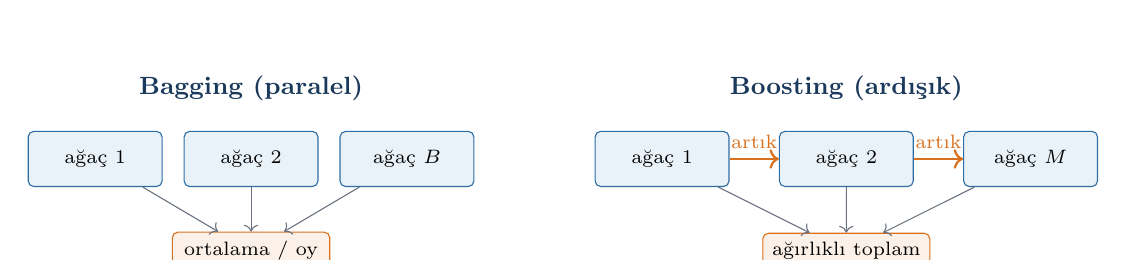
\begin{tikzpicture}[scale=0.9, every node/.style={font=\scriptsize},
  kutu/.style={draw=vurguMavi,fill=acikMavi,rounded corners=2pt,
               minimum width=1.7cm,minimum height=0.7cm,align=center}]
\node[font=\small\bfseries,anaMavi] at (2.2,2.6) {Bagging (paralel)};
\node[kutu] (v1) at (0,1.6) {ağaç 1};
\node[kutu] (v2) at (2.2,1.6) {ağaç 2};
\node[kutu] (v3) at (4.4,1.6) {ağaç $B$};
\node[draw=turuncu,fill=turuncu!10,rounded corners=2pt,minimum width=2cm] (o1) at (2.2,0.3) {ortalama / oy};
\draw[->,ortaGri] (v1)--(o1); \draw[->,ortaGri] (v2)--(o1); \draw[->,ortaGri] (v3)--(o1);
\node[font=\small\bfseries,anaMavi] at (10.6,2.6) {Boosting (ardışık)};
\node[kutu] (b1) at (8.0,1.6) {ağaç 1};
\node[kutu] (b2) at (10.6,1.6) {ağaç 2};
\node[kutu] (b3) at (13.2,1.6) {ağaç $M$};
\draw[->,turuncu,thick] (b1)--node[above]{artık}(b2);
\draw[->,turuncu,thick] (b2)--node[above]{artık}(b3);
\node[draw=turuncu,fill=turuncu!10,rounded corners=2pt,minimum width=2cm] (o2) at (10.6,0.3) {ağırlıklı toplam};
\draw[->,ortaGri] (b1)--(o2); \draw[->,ortaGri] (b2)--(o2); \draw[->,ortaGri] (b3)--(o2);
\end{tikzpicture}
\end{center}
\vspace{0.3cm}

\begin{center}
\begin{tabularx}{\textwidth}{@{}>{\bfseries\color{anaMavi}}l >{\raggedright\arraybackslash}X >{\raggedright\arraybackslash}X@{}}
\toprule
\rowcolor{acikMavi}\multicolumn{1}{@{}l}{\color{anaMavi}\textbf{Yöntem}} & \multicolumn{1}{l}{\color{anaMavi}\textbf{Fikir}} & \multicolumn{1}{l@{}}{\color{anaMavi}\textbf{Azalttığı}}\\
\midrule
Bagging & Bootstrap örneklerinde bağımsız modeller & Varyans\\
\rowcolor{acikGri} Random Forest & Bagging + her bölmede rastgele öznitelik alt kümesi & Varyans (ağaçları decorrelate eder)\\
Boosting & Her model öncekinin hatasına odaklanır & Yanlılık (ve varyans)\\
\rowcolor{acikGri} Stacking & Model tahminlerini bir üst model birleştirir & Her ikisi\\
\bottomrule
\end{tabularx}
\end{center}

\begin{lstlisting}
rf = RandomForestClassifier(n_estimators=300, random_state=42, n_jobs=-1).fit(X, y)
imp = pd.Series(rf.feature_importances_, index=X.columns).sort_values(ascending=False)
print(imp.head(8).round(4))
\end{lstlisting}

\begin{lstlisting}[style=outstyle]
worst perimeter         0.1476
worst area              0.1373
worst concave points    0.1209
mean concave points     0.0962
worst radius            0.0716
mean perimeter          0.0508
mean concavity          0.0486
mean radius             0.0478
\end{lstlisting}

\uyari{\code{feature\_importances\_} (Gini önemi) \textbf{yanlıdır}: yüksek
kardinaliteli ve sürekli değişkenleri şişirir, korelasyonlu özniteliklerin
önemini keyfi biçimde birine yükler. Güvenilir alternatif
\emph{permütasyon önemi} veya SHAP değerleridir (Kısım 11).}

\gsub{Voting ve Stacking}

\begin{lstlisting}
from sklearn.ensemble import VotingClassifier, StackingClassifier

temel = [('lr', make_pipeline(StandardScaler(), LogisticRegression(max_iter=5000))),
         ('rf', RandomForestClassifier(n_estimators=300, random_state=42)),
         ('gb', GradientBoostingClassifier(random_state=42))]

vote  = VotingClassifier(temel, voting='soft')
stack = StackingClassifier(temel, final_estimator=LogisticRegression(max_iter=1000), cv=5)

for ad, m in [('VotingSoft', vote), ('Stacking', stack)]:
    print(f"{ad}: roc_auc = {cross_val_score(m, X, y, cv=cv, scoring='roc_auc', n_jobs=-1).mean():.4f}")
\end{lstlisting}

\begin{lstlisting}[style=outstyle]
VotingSoft: roc_auc = 0.9948
Stacking: roc_auc = 0.9952
\end{lstlisting}

\bilgi{Topluluklar burada tek başına lojistik regresyonu ($0{,}9953$)
geçemedi. Topluluklar, temel modeller \emph{farklı hatalar} yaptığında işe
yarar; hepsi aynı yönde yanılıyorsa birleştirmek fayda etmez. Yine de
gerçek dünyada (özellikle tablo verisinde) gradient boosting ve stacking
genelde kazanır --- bu veri seti fazla ``kolay''.}

% =====================================================================
\gsec{Hiperparametre Ayarı}
% =====================================================================

\nicin[Parametre ile Hiperparametre Farkı]{\textbf{Parametreler} modelin
veriden \emph{öğrendiği} sayılardır --- regresyon katsayıları, sinir ağı
ağırlıkları. Bunları sen belirlemezsin, \code{fit()} belirler.
\textbf{Hiperparametreler} ise eğitimden \emph{önce} senin belirlemen gereken
ayarlardır --- ağaç derinliği, $k$ komşu sayısı, SVM'in $C$'si, öğrenme hızı,
düzenlileştirme gücü.

\textbf{Niçin bu kadar önemli?} Çünkü hemen hepsi doğrudan
\emph{yanlılık--varyans} düğmesidir. $k$-NN'de $k$, ağaçta \code{max\_depth},
Ridge'de $\alpha$, SVM'de $C$ --- hepsi aynı şeyi kontrol eder: modelin ne
kadar esnek olacağını. Yanlış ayarlanmış bir hiperparametre, doğru seçilmiş
bir algoritmayı işe yaramaz hâle getirir; SVM örneğinde $C=0{,}01$ ile \%62,
$C=10$ ile \%98 doğruluk almıştık --- aynı algoritma.

\textbf{Üç arama stratejisi:}
\begin{itemize}\itemsep1pt
\item \textbf{Izgara araması (\code{GridSearchCV}):} Tüm kombinasyonları
dener. Kesin ama üstel pahalıdır --- 3 parametrenin her biri 5 değer $\to$
125 model $\times$ 5 katman $=625$ eğitim. Az sayıda parametre varsa uygundur.
\item \textbf{Rastgele arama (\code{RandomizedSearchCV}):} Rastgele
kombinasyonlar dener. Şaşırtıcı biçimde ızgaradan \emph{daha verimlidir},
çünkü genellikle parametrelerin yalnızca birkaçı gerçekten önemlidir ve
rastgele arama o birkaçı daha çok farklı değerde dener. Varsayılan tercihin
bu olsun.
\item \textbf{Bayesçi optimizasyon (Optuna, \code{skopt}):} Önceki
denemelerden öğrenerek nereye bakacağına karar verir. Pahalı modellerde
(derin öğrenme, büyük veri) en verimli yöntemdir --- ve mantığı doğrudan
Kısım 6'daki Bayesçi güncellemedir.
\end{itemize}

\textbf{En kritik kural --- test kümesine dokunma.} Hiperparametre araması,
\emph{eğitim} verisi üzerindeki çapraz doğrulama ile yapılır. Test kümesine
bakarak ayar yaparsan, test skorun artık dürüst bir tahmin değildir ---
farkında olmadan test kümesine aşırı uydurmuş olursun. Hem model seçip hem
performans ölçmen gerekiyorsa \emph{iç içe (nested) çapraz doğrulama}
kullanılır; aşağıdaki kod tam olarak bunu gösteriyor.

\textbf{Pratik öncelik:} Sonsuz parametre aramak yerine, önce hangilerinin
önemli olduğunu bil. Gradyan artırmada \code{learning\_rate} ve
\code{n\_estimators}; rastgele ormanda \code{max\_features} ve
\code{min\_samples\_leaf}; SVM'de $C$ ve $\gamma$. Geri kalanı genellikle
varsayılanda bırakılabilir. Ve unutma: \textbf{daha iyi öznitelik, daha iyi
hiperparametreden neredeyse her zaman daha değerlidir.}}

\begin{lstlisting}
from sklearn.model_selection import GridSearchCV, RandomizedSearchCV

grid = GridSearchCV(
    make_pipeline(StandardScaler(), SVC(random_state=42)),
    {'svc__C': [0.1, 1, 10, 100], 'svc__gamma': ['scale', 0.01, 0.1, 1]},
    cv=cv, scoring='roc_auc', n_jobs=-1)
grid.fit(X, y)
print("en iyi parametreler:", grid.best_params_)
print(f"en iyi CV roc_auc  = {grid.best_score_:.4f}")
\end{lstlisting}

\begin{lstlisting}[style=outstyle]
en iyi parametreler: {'svc__C': 10, 'svc__gamma': 0.01}
en iyi CV roc_auc  = 0.9960
\end{lstlisting}

\begin{center}
\begin{tabularx}{\textwidth}{@{}>{\ttfamily\color{anaMavi}}l >{\raggedright\arraybackslash}X@{}}
\toprule
\rowcolor{acikMavi}\multicolumn{1}{@{}l}{\color{anaMavi}\textbf{Yöntem}} & \multicolumn{1}{l@{}}{\color{anaMavi}\textbf{Ne zaman?}}\\
\midrule
GridSearchCV & Az sayıda parametre, küçük ızgara.\\
\rowcolor{acikGri} RandomizedSearchCV & Çok parametre; aynı bütçeyle genelde daha iyi sonuç.\\
HalvingGridSearchCV & Ardışık eleme; büyük ızgaralarda hızlı.\\
\rowcolor{acikGri} optuna / hyperopt & Bayesçi optimizasyon; pahalı modellerde en verimli.\\
\bottomrule
\end{tabularx}
\end{center}

\uyari{\textbf{Yuvalanmış (nested) CV}: hiperparametreyi CV ile seçip aynı
CV skorunu ``model performansı'' diye raporlamak iyimser yanlılık üretir.
Dürüst kestirim için dış döngü (performans) ile iç döngü (ayar) ayrılmalıdır:
\code{cross\_val\_score(GridSearchCV(...), X, y, cv=dis\_cv)}.}

\begin{lstlisting}
# Yuvalanmis CV: durust performans kestirimi
from sklearn.model_selection import cross_val_score as cvs
ic_cv  = StratifiedKFold(4, shuffle=True, random_state=1)
dis_cv = StratifiedKFold(5, shuffle=True, random_state=2)
arayici = GridSearchCV(make_pipeline(StandardScaler(), SVC(random_state=42)),
                       {'svc__C': [0.1, 1, 10, 100]}, cv=ic_cv, scoring='roc_auc')
print(f"yuvalanmis CV roc_auc = {cvs(arayici, X, y, cv=dis_cv, scoring='roc_auc').mean():.4f}")
\end{lstlisting}

\gsub{Boosting Kütüphaneleri}

\begin{center}
\begin{tabularx}{\textwidth}{@{}>{\bfseries\color{anaMavi}}l >{\raggedright\arraybackslash}X@{}}
\toprule
\rowcolor{acikMavi}\multicolumn{1}{@{}l}{\color{anaMavi}\textbf{Kütüphane}} & \multicolumn{1}{l@{}}{\color{anaMavi}\textbf{Özellik}}\\
\midrule
HistGradientBoosting & scikit-learn içinde; hızlı, eksik değeri kendi işler.\\
\rowcolor{acikGri} XGBoost & Olgun, düzenlileştirme güçlü, GPU desteği.\\
LightGBM & Çok hızlı, büyük veride tercih; yaprak-bazlı büyüme.\\
\rowcolor{acikGri} CatBoost & Kategorik değişkenleri doğrudan işler; ayarsız iyi çalışır.\\
\bottomrule
\end{tabularx}
\end{center}

\begin{lstlisting}
# Tipik XGBoost/LightGBM baslangic parametreleri
params = dict(
    n_estimators=1000, learning_rate=0.05, max_depth=6,
    subsample=0.8, colsample_bytree=0.8,
    reg_lambda=1.0, early_stopping_rounds=50, random_state=42)
# Kural: learning_rate kucultursen n_estimators buyut (ters orantili).
\end{lstlisting}

% #####################################################################
\gpart{10}{Denetimsiz Öğrenme}
% #####################################################################

% =====================================================================
\gsec{K-Means Kümeleme}
% =====================================================================

\form[Amaç Fonksiyonu]{Küme içi kareler toplamını (inertia) minimize et:
\[
J=\sum_{i=1}^{n}\min_{c}\|x_i-\mu_c\|^2 .
\]
Lloyd algoritması iki adımı yineler: (1) her noktayı en yakın merkeze ata,
(2) merkezleri atanan noktaların ortalaması yap.}

\nicin{\textbf{Kümeleme hangi soruyu cevaplar?} Şimdiye kadarki her modelde
bir ``doğru cevap'' (etiket) vardı. Kümelemede yoktur --- elinde sadece veri
var ve soru şu: \emph{``Bu veride doğal olarak kaç grup var ve hangi
gözlemler birbirine benziyor?''} Etiket olmadan öğrendiği için
\textbf{denetimsiz} öğrenme denir.

\textbf{$J$ formülü ne diyor?} Her noktanın, ait olduğu kümenin merkezine
uzaklığının karesi --- hepsi toplanır. Küçük $J$ demek, ``noktalar kendi
merkezlerine sıkıca yapışmış'' demektir. Algoritma bu toplamı en küçük yapan
küme atamasını arar.

\textbf{Lloyd algoritması niçin işe yarıyor?} İki adım da $J$'yi asla
artırmaz: (1) her noktayı en yakın merkeze atamak, o noktanın katkısını
küçültür; (2) merkezi ortalamaya taşımak, o kümenin kareler toplamını
küçültür (Kısım 2: ortalama, karesel sapmayı minimize eden noktadır). Sürekli
azalan ve alttan sınırlı bir dizi olduğu için mutlaka durur. Ama
\textbf{yerel} bir minimuma takılabilir --- bu yüzden \code{n\_init} ile
farklı başlangıçlardan defalarca çalıştırılır.

\textbf{$k$'yı kim seçiyor?} Sen. Ve bu, K-Means'in en büyük zorluğudur.
Yardımcı araçlar: \emph{dirsek yöntemi} ($J$'nin düşüş hızının kırıldığı
nokta), \emph{siluet skoru} (noktalar kendi kümesine mi yoksa komşusuna mı
daha yakın?), ve --- en önemlisi --- \emph{alan bilgisi}. ``Pazarlama ekibi
4 segmentle çalışabilir'' cümlesi çoğu zaman siluet skorundan daha
belirleyicidir.

\textbf{Varsayımları (ve ne zaman kırıldığı):}
\begin{itemize}\itemsep1pt
\item Kümeler \emph{küresel} ve benzer büyüklüktedir. Uzun, ince veya iç içe
kümelerde başarısız olur --- o zaman DBSCAN veya spektral kümeleme gerekir.
\item Uzaklık temellidir, dolayısıyla \textbf{ölçekleme zorunludur}.
\item Her nokta bir kümeye atanır; aykırı değerler bir kümeye zorla girer ve
merkezi çeker. Aykırı değer varsa K-Medoids daha güvenlidir.
\end{itemize}

\textbf{Nerede kullanılır?}
\begin{itemize}\itemsep1pt
\item \textbf{Müşteri segmentasyonu:} RFM (recency--frequency--monetary)
verisiyle müşterileri gruplara ayırmak --- pazarlamanın en yaygın veri
bilimi uygulaması.
\item \textbf{Görüntü sıkıştırma:} Milyonlarca rengi 16 renge indirmek ---
her piksel en yakın küme merkezine yuvarlanır (renk nicemleme).
\item \textbf{Belge/haber gruplama:} Benzer içerikleri otomatik toplamak.
\item \textbf{Anomali tespiti:} Hiçbir merkeze yakın olmayan noktalar şüpheli.
\item \textbf{Öznitelik mühendisliği:} Küme numarasını yeni bir kategorik
öznitelik olarak denetimli modele vermek.
\end{itemize}

\textbf{Önemli uyarı:} K-Means \emph{her zaman} $k$ küme bulur --- veri
tamamen homojen olsa bile. ``Küme buldum'' demek ``gerçekten grup var''
demek değildir. Bulunan kümelerin anlamlı olup olmadığını her zaman alan
bilgisiyle doğrula.}

\begin{lstlisting}
import numpy as np, pandas as pd
from sklearn.datasets import load_wine
from sklearn.preprocessing import StandardScaler
from sklearn.cluster import KMeans
from sklearn.metrics import (silhouette_score, adjusted_rand_score,
                             calinski_harabasz_score, davies_bouldin_score)

wine = load_wine(as_frame=True); Xw, yw = wine.data, wine.target
Xs = StandardScaler().fit_transform(Xw)          # OLCEKLEME SART

for k in range(2, 8):
    km = KMeans(k, n_init=10, random_state=42).fit(Xs)
    print(f"k={k}: inertia={km.inertia_:8.1f}  silhouette={silhouette_score(Xs, km.labels_):.4f}"
          f"  CH={calinski_harabasz_score(Xs, km.labels_):7.1f}"
          f"  DB={davies_bouldin_score(Xs, km.labels_):.4f}")
\end{lstlisting}

\begin{lstlisting}[style=outstyle]
k=2: inertia=  1658.8  silhouette=0.2593  CH=   69.5  DB=1.5260
k=3: inertia=  1277.9  silhouette=0.2849  CH=   70.9  DB=1.3892
k=4: inertia=  1175.4  silhouette=0.2602  CH=   56.2  DB=1.7969
k=5: inertia=  1109.5  silhouette=0.2016  CH=   47.0  DB=1.8083
k=6: inertia=  1046.0  silhouette=0.2372  CH=   41.7  DB=1.5544
k=7: inertia=   981.6  silhouette=0.2036  CH=   38.7  DB=1.6606
\end{lstlisting}

\begin{center}
\begin{tabularx}{\textwidth}{@{}>{\bfseries\color{anaMavi}}l >{\raggedright\arraybackslash}X >{\raggedright\arraybackslash}X@{}}
\toprule
\rowcolor{acikMavi}\multicolumn{1}{@{}l}{\color{anaMavi}\textbf{Ölçüt}} & \multicolumn{1}{l}{\color{anaMavi}\textbf{Yorum}} & \multicolumn{1}{l@{}}{\color{anaMavi}\textbf{Yön}}\\
\midrule
Inertia (elbow) & Küme içi yayılım & Küçük iyi; ama $k$ ile hep düşer $\to$ dirsek ara\\
\rowcolor{acikGri} Silhouette & Kendi kümesine yakınlık / diğerlerine uzaklık & $[-1,1]$, büyük iyi\\
Calinski--Harabasz & Gruplar arası / grup içi varyans & Büyük iyi\\
\rowcolor{acikGri} Davies--Bouldin & Küme benzerliği & Küçük iyi\\
ARI & Gerçek etiketlerle uyum (varsa) & $[-1,1]$, büyük iyi\\
\bottomrule
\end{tabularx}
\end{center}

Üç iç ölçüt de $k=3$'ü işaret ediyor --- ve şarap veri setinde gerçekten 3
üzüm çeşidi var.

\begin{lstlisting}
km3 = KMeans(3, n_init=10, random_state=42).fit(Xs)
print(f"ARI (gercek siniflarla) = {adjusted_rand_score(yw, km3.labels_):.4f}")
print(pd.crosstab(yw, km3.labels_))
\end{lstlisting}

\begin{lstlisting}[style=outstyle]
ARI (gercek siniflarla) = 0.8975
col_0    0   1   2
target            
0        0   0  59
1       65   3   3
2        0  48   0
\end{lstlisting}

\bilgi{Etiketleri hiç görmeden, yalnızca kimyasal ölçümlerden üç üzüm
çeşidinin 178 örneğinin 172'si doğru gruplandı (ARI $=0{,}90$). Kümeleme
etiket üretmez, \emph{yapı} bulur; etiketle eşleştirme senin yorumundur.}

\uyari{K-Means'in varsayımları: küresel, benzer boyutlu, benzer yoğunluklu
kümeler. Uzamış, iç içe geçmiş veya farklı yoğunluktaki kümelerde başarısız
olur. Ayrıca \code{n\_init} varsayılanı yetersizse kötü yerel minimuma
takılır --- her zaman \code{n\_init=10} veya daha fazlasını ver.}

% =====================================================================
\gsec{Diğer Kümeleme Yöntemleri}
% =====================================================================

\begin{center}
\begin{tabularx}{\textwidth}{@{}>{\bfseries\color{anaMavi}}l >{\raggedright\arraybackslash}X >{\raggedright\arraybackslash}X@{}}
\toprule
\rowcolor{acikMavi}\multicolumn{1}{@{}l}{\color{anaMavi}\textbf{Yöntem}} & \multicolumn{1}{l}{\color{anaMavi}\textbf{Fikir}} & \multicolumn{1}{l@{}}{\color{anaMavi}\textbf{Avantaj / kısıt}}\\
\midrule
K-Means & Merkezlere uzaklık & Hızlı; $k$ verilmeli, küresel kümeler\\
\rowcolor{acikGri} Hiyerarşik & Ardışık birleştirme & Dendrogram; $k$ sonradan seçilir, $O(n^2)$\\
DBSCAN & Yoğunluk temelli & Rastgele şekil, gürültü tespiti; \code{eps} hassas\\
\rowcolor{acikGri} GMM & Olasılıksal karışım & Elips kümeler, yumuşak atama, BIC ile $k$\\
Spektral & Grafik Laplacian & İç içe geçmiş kümeler; pahalı\\
\bottomrule
\end{tabularx}
\end{center}

\begin{lstlisting}
from sklearn.cluster import AgglomerativeClustering, DBSCAN
from sklearn.mixture import GaussianMixture

ag = AgglomerativeClustering(3).fit(Xs)
print(f"Agglomerative ARI = {adjusted_rand_score(yw, ag.labels_):.4f}")

for eps in [1.5, 2.0, 2.5, 3.0]:
    db = DBSCAN(eps=eps, min_samples=5).fit(Xs)
    nk = len(set(db.labels_)) - (1 if -1 in db.labels_ else 0)
    print(f"DBSCAN eps={eps}: kume={nk}  gurultu={(db.labels_==-1).sum():3d}  "
          f"ARI={adjusted_rand_score(yw, db.labels_):.4f}")

for k in range(1, 7):
    g = GaussianMixture(k, random_state=42, n_init=3).fit(Xs)
    print(f"GMM k={k}: BIC={g.bic(Xs):8.1f}   AIC={g.aic(Xs):8.1f}")
\end{lstlisting}

\begin{lstlisting}[style=outstyle]
Agglomerative ARI = 0.7899
DBSCAN eps=1.5: kume=0  gurultu=178  ARI=0.0000
DBSCAN eps=2.0: kume=5  gurultu= 85  ARI=0.2205
DBSCAN eps=2.5: kume=1  gurultu= 24  ARI=0.0050
DBSCAN eps=3.0: kume=1  gurultu= 11  ARI=-0.0059
GMM k=1: BIC=  5741.3   AIC=  5410.4
GMM k=2: BIC=  5629.6   AIC=  4964.6
GMM k=3: BIC=  5806.3   AIC=  4807.2
GMM k=4: BIC=  5806.8   AIC=  4473.7
GMM k=5: BIC=  6360.4   AIC=  4693.1
GMM k=6: BIC=  6752.7   AIC=  4751.3
\end{lstlisting}

\uyari{Bu 13 boyutlu veride \textbf{DBSCAN tamamen başarısız}: yüksek boyutta
yoğunluk kavramı anlamını yitirir (boyut laneti) ve \code{eps} için işe yarar
bir değer yoktur. DBSCAN'i düşük boyutlu, yoğunluk farkı belirgin verilerde
kullan --- ya da önce PCA ile boyut indir.}

\bilgi{GMM'de BIC $k=2$'yi, AIC ise daha büyük $k$'ları seçiyor. BIC daha
muhafazakârdır (karmaşıklığı $\log n$ ile cezalandırır), AIC daha cömerttir.
Küme sayısı gibi \emph{yapısal} kararlarda BIC tercih edilir.}

% =====================================================================
\gsec{Boyut İndirgeme: PCA}
% =====================================================================

\form[PCA]{Veriyi, varyansı en çok koruyan dik eksenlere yansıtır. Bu eksenler
kovaryans matrisinin özvektörleridir; açıklanan varyans oranları da
özdeğerlerdir:
\[
\Sigma = \frac{1}{n-1}X^\top X,
\qquad
\Sigma v_j=\lambda_j v_j,
\qquad
\text{açıklanan oran}_j=\frac{\lambda_j}{\sum_k\lambda_k}.
\]}

\nicin{\textbf{Hangi problemi çözüyor?} 30 öznitelikli bir veriyi
göremezsin, ve öznitelikler birbiriyle ilişkiliyse çoğu \emph{aynı bilgiyi
tekrar tekrar} taşıyordur. PCA, bu tekrarı sıkıştırır: ilişkili birçok
değişkeni, birbiriyle ilişkisiz az sayıda ``bileşene'' indirir.

\textbf{Sezgi --- gölge benzetmesi.} Elinde üç boyutlu bir nesne var ve onu
duvara yansıtacaksın. Hangi açıdan tutarsan gölge en çok bilgi taşır?
Nesnenin en \emph{uzun} olduğu yönden. PCA tam olarak bunu yapar: verinin en
çok yayıldığı yönü bulur (birinci bileşen), sonra ona \emph{dik} olan
yönlerden en çok yayılanı (ikinci bileşen), ve böyle devam eder.

\textbf{Niçin ``en çok varyans'' iyi bir ölçüt?} Çünkü varyans $=$ bilgi.
Bütün gözlemlerde aynı olan bir değişken hiçbir şey ayırt etmez; çok değişen
bir değişken çok şey ayırt eder. En az varyanslı yönleri atmak, en az bilgi
kaybetmek demektir.

\textbf{Özvektör--özdeğer bağlantısı nereden geliyor?} ``Varyansı en büyük
yapan yön'' problemi, kovaryans matrisinin en büyük özdeğerine karşılık gelen
özvektörü bulmakla \emph{aynı problemdir}. Özdeğer $\lambda_j$, o yöndeki
varyansın kendisidir --- bu yüzden ``açıklanan oran'' basitçe
$\lambda_j$'nin toplama bölümüdür.

\textbf{Kaç bileşen tutmalı?} Üç ölçüt: (1) kümülatif açıklanan varyans
\%90--95'i geçene kadar; (2) scree grafiğinde dirsek noktası; (3) sonraki
modelin çapraz doğrulama skoru --- en dürüst ölçüt budur.

\textbf{Nerede kullanılır?}
\begin{itemize}\itemsep1pt
\item \textbf{Görselleştirme:} 50 boyutlu veriyi 2 boyuta indirip gruplaşmayı
gözle görmek.
\item \textbf{Gürültü azaltma:} Küçük özdeğerli bileşenler genellikle
gürültüdür; atınca sinyal temizlenir. Görüntü ve sinyal işlemede standarttır.
\item \textbf{Çoklu bağlantı çözümü:} Bileşenler tanımı gereği ilişkisizdir,
dolayısıyla regresyondaki VIF sorununu bitirir (\emph{temel bileşen
regresyonu}).
\item \textbf{Hız:} 10.000 öznitelikli veriyi 100 bileşene indirip modeli
100 kat hızlandırmak.
\item \textbf{Yüz tanıma:} Klasik ``eigenfaces'' yöntemi doğrudan PCA'dır.
\item \textbf{Finans:} Faiz oranı eğrisinin \%95'i üç bileşenle açıklanır:
seviye, eğim ve eğrilik. Tüm tahvil risk yönetimi bu ayrıştırma üzerine
kuruludur.
\end{itemize}

\textbf{Bedeli nedir?} \emph{Yorumlanabilirlik}. ``PC1'' artık ``metrekare''
gibi anlamlı bir şey değil, tüm değişkenlerin ağırlıklı bir karışımıdır.
Bileşenleri anlamanın tek yolu \emph{yüklemelere} (loadings) bakmaktır ---
hangi değişkenler o bileşene çok katkı yapıyor? Aşağıdaki kod tam olarak
bunu yapıyor.}

\begin{lstlisting}
from sklearn.decomposition import PCA
p = PCA().fit(Xs)
print("aciklanan varyans (ilk 6):", np.round(p.explained_variance_ratio_[:6], 4))
print("kumulatif                :", np.round(np.cumsum(p.explained_variance_ratio_)[:6], 4))
n95 = np.searchsorted(np.cumsum(p.explained_variance_ratio_), 0.95) + 1
print(f"%95 varyans icin bilesen sayisi = {n95}")
\end{lstlisting}

\begin{lstlisting}[style=outstyle]
aciklanan varyans (ilk 6): [0.362  0.1921 0.1112 0.0707 0.0656 0.0494]
kumulatif                : [0.362  0.5541 0.6653 0.736  0.8016 0.851 ]
%95 varyans icin bilesen sayisi = 10
\end{lstlisting}

\begin{lstlisting}
# Yuklemeler (loadings): bilesenleri YORUMLAMANIN tek yolu
p2 = PCA(2).fit(Xs)
yuk = pd.DataFrame(p2.components_.T, index=Xw.columns, columns=['PC1','PC2'])
print(yuk.round(3))
\end{lstlisting}

\begin{lstlisting}[style=outstyle]
                                PC1    PC2
alcohol                       0.144  0.484
malic_acid                   -0.245  0.225
ash                          -0.002  0.316
alcalinity_of_ash            -0.239 -0.011
magnesium                     0.142  0.300
total_phenols                 0.395  0.065
flavanoids                    0.423 -0.003
nonflavanoid_phenols         -0.299  0.029
proanthocyanins               0.313  0.039
color_intensity              -0.089  0.530
hue                           0.297 -0.279
od280/od315_of_diluted_wines  0.376 -0.164
proline                       0.287  0.365
\end{lstlisting}

\bilgi{PC1'e en çok katkı veren değişkenler \code{flavanoids} ($0{,}42$),
\code{total\_phenols} ($0{,}40$) ve \code{od280} ($0{,}38$) --- yani PC1 bir
\emph{``fenolik zenginlik'' ekseni}. PC2 ise \code{color\_intensity} ($0{,}53$)
ve \code{alcohol} ($0{,}48$) ile yüklü: \emph{``gövde/renk'' ekseni}. Bileşenler
ancak yüklemeler okunarak yorumlanır.}

\uyari{PCA \textbf{ölçeklemeye bağımlıdır}: ölçeklemezsen en büyük birimli
değişken (burada \code{proline}, binlerce birim) tüm varyansı domine eder ve
PCA anlamsızlaşır. Ayrıca PCA \emph{denetimsizdir}: en çok varyans taşıyan
yön, sınıfları en iyi ayıran yön olmak zorunda değildir --- o iş için LDA
kullanılır.}

\gsub{t-SNE ve UMAP: Görselleştirme İçin}

\begin{lstlisting}
from sklearn.manifold import TSNE
from sklearn.datasets import load_digits

digits = load_digits()
Z = TSNE(n_components=2, perplexity=30, init='pca', random_state=42).fit_transform(digits.data)

import matplotlib.pyplot as plt
plt.figure(figsize=(7, 6))
sc = plt.scatter(Z[:,0], Z[:,1], c=digits.target, cmap='tab10', s=8)
plt.colorbar(sc); plt.title('digits: t-SNE'); plt.show()
\end{lstlisting}

\uyari{t-SNE ve UMAP yalnızca \textbf{görselleştirme} içindir:
(1) kümeler arası \emph{uzaklıklar} anlamlı değildir, (2) küme
\emph{boyutları} anlamlı değildir, (3) \code{perplexity}'yi değiştirince
görüntü değişir, (4) \code{transform} yoktur --- yeni veriye uygulanamaz.
Boyut indirgemeyi bir modelin ön işleme adımı yapacaksan PCA kullan.}

% =====================================================================
\gsec{Anomali Tespiti}
% =====================================================================

\begin{lstlisting}
from sklearn.ensemble import IsolationForest
from sklearn.neighbors import LocalOutlierFactor
from sklearn.datasets import load_breast_cancer

bc = load_breast_cancer()
Xb = StandardScaler().fit_transform(bc.data)

iso  = IsolationForest(contamination=0.05, random_state=42).fit(Xb)
pred = iso.predict(Xb)                                # -1: anomali
print(f"IsolationForest anomali = {(pred==-1).sum()} / {len(pred)}")
print(f"anomalilerin gercek sinif dagilimi = {np.bincount(bc.target[pred==-1])}")

lof = LocalOutlierFactor(n_neighbors=20, contamination=0.05).fit_predict(Xb)
print(f"LOF anomali = {(lof==-1).sum()}")
\end{lstlisting}

\begin{lstlisting}[style=outstyle]
IsolationForest anomali = 29 / 569
anomalilerin gercek sinif dagilimi = [22  7]
LOF anomali = 29
\end{lstlisting}

\bilgi{Tespit edilen 29 anomalinin 22'si kötü huylu tümör (sınıf 0) ---
etiketler hiç kullanılmadan. Anomali tespiti, etiketli veri bulmanın zor
olduğu alanlarda (dolandırıcılık, arıza, siber saldırı) tam olarak bu yüzden
kullanılır: ``normal''i öğrenip sapanları işaretler.}

\begin{center}
\begin{tabularx}{\textwidth}{@{}>{\ttfamily\color{anaMavi}}l >{\raggedright\arraybackslash}X@{}}
\toprule
\rowcolor{acikMavi}\multicolumn{1}{@{}l}{\color{anaMavi}\textbf{Yöntem}} & \multicolumn{1}{l@{}}{\color{anaMavi}\textbf{Ne zaman?}}\\
\midrule
IsolationForest & Genel amaçlı, yüksek boyut, hızlı. Varsayılan tercih.\\
\rowcolor{acikGri} LocalOutlierFactor & Yerel yoğunluk farkları önemliyse.\\
OneClassSVM & Küçük veri, karmaşık sınır; ölçeklemeye duyarlı.\\
\rowcolor{acikGri} EllipticEnvelope & Veri yaklaşık normal ve tek tepeliyse.\\
\bottomrule
\end{tabularx}
\end{center}

% #####################################################################
\gpart{11}{İleri Konular}
% #####################################################################

% =====================================================================
\gsec{Dengesiz Veri}
% =====================================================================

Dolandırıcılık, nadir hastalık, makine arızası --- gerçek problemlerin çoğunda
ilgilendiğimiz sınıf \%1--5 orandadır. Bu, ``doğruluk'' metriğini işe
yaramaz hâle getirir.

\nicin[Dengesizlik Niçin Bir Sorun?]{Bir model, kaybı minimize etmeye
çalışır. Pozitif sınıf \%2 ise, ``hepsine negatif de'' stratejisi \%98
doğruluk verir --- ve model bunu bulmakta hiç zorlanmaz. Sorun modelin
kötü olması değil; \textbf{ona sorduğun sorunun yanlış olmasıdır.}

Bu, Kısım 3'teki \emph{taban oranı yanılgısının} makine öğrenmesindeki
karşılığıdır ve aynı sonucu doğurur: nadir bir olayda, iyi bir sınıflandırıcı
bile çok sayıda yanlış pozitif üretir.

\textbf{Dört müdahale yolu --- ve hangisi ne zaman:}
\begin{itemize}\itemsep2pt
\item \textbf{Metriği değiştir (her zaman yap).} Doğruluk yerine PR-AUC,
duyarlılık, F1 veya doğrudan iş maliyeti. Bu, en ucuz ve en etkili adımdır ---
çoğu ``dengesiz veri sorunu'', aslında ``yanlış metrik sorunudur''.
\item \textbf{Sınıf ağırlığı (\code{class\_weight='balanced'}).} Azınlık
sınıfının hatalarını kayıp fonksiyonunda daha ağır say. Veriye
dokunmadığı için en temiz çözümdür; ilk deneyeceğin şey olsun.
\item \textbf{Yeniden örnekleme (SMOTE, alt/üst örnekleme).} Azınlık sınıfını
çoğalt veya çoğunluğu azalt. \emph{Kritik uyarı:} bu işlem yalnızca
\textbf{eğitim} katmanında yapılmalıdır. Bölmeden önce SMOTE uygularsan
sentetik örnekler test kümesine sızar ve skorların anlamsızlaşır ---
\code{imblearn.pipeline.Pipeline} bunu doğru yapar.
\item \textbf{Karar eşiğini ayarla.} Genellikle en yüksek getirili ve en çok
ihmal edilen adım. Model zaten iyi olasılıklar üretiyor olabilir; sorun
$0{,}5$ eşiğinin bu problem için yanlış olmasıdır. Bir sonraki alt bölümün
konusu budur.
\end{itemize}

\textbf{Önemli nüans:} Dengesizlik \emph{her zaman} bir sorun değildir.
Eğer modelin ürettiği olasılıklar iyiyse ve sen sıralamayla ilgileniyorsan
(``en riskli 100 işlemi incele''), hiçbir müdahaleye gerek yoktur. Dahası,
yeniden örnekleme olasılıkları bozar --- kalibrasyon önemliyse ondan kaçın.

\textbf{Nerede karşına çıkar?} Dolandırıcılık tespiti (\%0,1 pozitif),
tıbbi tarama, üretimde kusur tespiti, müşteri kaybı tahmini, reklam tıklama
tahmini (\%0,5 CTR), ağ saldırısı tespiti --- yani gerçek dünyadaki
problemlerin çoğunda.}

\begin{lstlisting}
import numpy as np, pandas as pd
from sklearn.datasets import make_classification
from sklearn.model_selection import train_test_split
from sklearn.dummy import DummyClassifier
from sklearn.linear_model import LogisticRegression
from sklearn.pipeline import make_pipeline
from sklearn.preprocessing import StandardScaler
from sklearn.metrics import (accuracy_score, precision_score, recall_score,
                             f1_score, roc_auc_score, average_precision_score)

X, y = make_classification(n_samples=10_000, n_features=20, n_informative=5,
                           weights=[0.98, 0.02], random_state=42)
print("sinif dagilimi:", np.bincount(y), f"pozitif oran = {y.mean():.4f}")
Xtr, Xte, ytr, yte = train_test_split(X, y, test_size=.3, random_state=42, stratify=y)

def rapor(ad, m):
    yh, yp = m.predict(Xte), m.predict_proba(Xte)[:, 1]
    print(f"{ad:>26}: acc={accuracy_score(yte,yh):.4f} "
          f"prec={precision_score(yte,yh,zero_division=0):.4f} rec={recall_score(yte,yh):.4f} "
          f"f1={f1_score(yte,yh):.4f} roc={roc_auc_score(yte,yp):.4f} "
          f"pr_auc={average_precision_score(yte,yp):.4f}")

rapor("hep-cogunluk (dummy)", DummyClassifier(strategy='most_frequent').fit(Xtr, ytr))
rapor("lojistik (duz)",
      make_pipeline(StandardScaler(), LogisticRegression(max_iter=2000, random_state=42)).fit(Xtr, ytr))
rapor("lojistik (class_weight)",
      make_pipeline(StandardScaler(), LogisticRegression(max_iter=2000,
                    class_weight='balanced', random_state=42)).fit(Xtr, ytr))
\end{lstlisting}

\begin{lstlisting}[style=outstyle]
sinif dagilimi: [9744  256] pozitif oran = 0.0256
      hep-cogunluk (dummy): acc=0.9743 prec=0.0000 rec=0.0000 f1=0.0000 roc=0.5000 pr_auc=0.0257
            lojistik (duz): acc=0.9743 prec=0.0000 rec=0.0000 f1=0.0000 roc=0.7590 pr_auc=0.1349
   lojistik (class_weight): acc=0.6860 prec=0.0555 rec=0.7013 f1=0.1029 roc=0.7481 pr_auc=0.1045
\end{lstlisting}

\uyari{``Her şeye negatif de'' diyen aptal model \textbf{\%97,43} doğruluk
alıyor --- ve eğitilmiş lojistik regresyon da tam olarak bunu yapıyor
(duyarlılık $=0$). Doğruluk burada tamamen anlamsızdır. Kullanılacak
metrikler: \textbf{PR-AUC}, duyarlılık, kesinlik ve iş maliyetine dayalı
özel bir skor.}

\begin{center}
\begin{tabularx}{\textwidth}{@{}>{\bfseries\color{anaMavi}}l >{\raggedright\arraybackslash}X@{}}
\toprule
\rowcolor{acikMavi}\multicolumn{1}{@{}l}{\color{anaMavi}\textbf{Strateji}} & \multicolumn{1}{l@{}}{\color{anaMavi}\textbf{Açıklama}}\\
\midrule
\code{class\_weight='balanced'} & Kayıp fonksiyonunda azınlığa daha büyük ağırlık. \textbf{İlk denenecek.}\\
\rowcolor{acikGri} Eşik ayarı & Karar eşiğini $0{,}5$'ten indir; model yeniden eğitilmez.\\
Rastgele alt örnekleme & Çoğunluğu azalt; hızlı ama bilgi kaybı.\\
\rowcolor{acikGri} SMOTE & Azınlık için sentetik örnek üret (\code{imbalanced-learn}); \emph{yalnız eğitim katlamasında}.\\
Maliyet duyarlı öğrenme & FP ve FN maliyetlerini doğrudan modele ver.\\
\rowcolor{acikGri} Anomali tespiti & Azınlık $<$\%1 ise sınıflandırma yerine anomali yaklaşımı.\\
\bottomrule
\end{tabularx}
\end{center}

\gsub{Eşik Ayarı: Bedava Kazanç}

\begin{lstlisting}
from sklearn.metrics import precision_recall_curve
m1 = make_pipeline(StandardScaler(), LogisticRegression(max_iter=2000, random_state=42)).fit(Xtr, ytr)
yp = m1.predict_proba(Xte)[:, 1]

prec, rec, thr = precision_recall_curve(yte, yp)
f1s = 2*prec*rec/(prec + rec + 1e-12)
i = np.nanargmax(f1s)
print(f"varsayilan esik 0.50 -> f1 = {f1_score(yte, (yp > 0.5).astype(int)):.4f}")
print(f"en iyi esik {thr[i]:.4f} -> f1 = {f1s[i]:.4f} "
      f"(kesinlik={prec[i]:.4f}, duyarlilik={rec[i]:.4f})")
\end{lstlisting}

\begin{lstlisting}[style=outstyle]
varsayilan esik 0.50 -> f1 = 0.0000
en iyi esik 0.0820 -> f1 = 0.2379 (kesinlik=0.1800, duyarlilik=0.3506)
\end{lstlisting}

\ipucu{Eşiği $0{,}5$'te bırakmak bir \emph{varsayılan}, bir karar değildir.
Doğru eşik, hataların \textbf{maliyetinden} çıkar: kanser taramasında FN
maliyeti FP'nin 100 katıysa eşik çok düşük olmalıdır. Eşiği eğitim/doğrulama
verisiyle seç, test verisiyle \emph{asla}.}

% =====================================================================
\gsec{Model Yorumlama}
% =====================================================================

\gsub{Permütasyon Önemi}

\form{Bir özniteliğin değerlerini rastgele karıştır; skor ne kadar düşerse o
öznitelik o kadar önemlidir. Model bağımsızdır, test verisinde hesaplanır ve
Gini öneminin yanlılıklarından muaftır.}

\nicin{\textbf{Fikir --- Kısım 6'daki permütasyon testinin ta kendisi.}
Mantık aynı: eğer bir öznitelik gerçekten işe yarıyorsa, değerlerini
karıştırıp anlamsızlaştırdığında model kötüleşmelidir. Kötüleşmiyorsa o
öznitelik zaten kullanılmıyordu.

\textbf{Niçin \emph{test} verisinde hesaplanır?} Çünkü sorduğun soru
``model bu özniteliğe ne kadar \emph{bel bağlıyor}?'' değil, ``bu öznitelik
\emph{gerçek} performansa ne kadar katkı yapıyor?''dur. Eğitim verisinde
hesaplarsan, ezberlenmiş gürültüyü de ``önemli'' sayarsın.

\textbf{Ağacın kendi (Gini) önemine niçin güvenilmez?} Üç sistematik
yanlılığı vardır: (1) çok değerli özniteliklere (sürekli değişkenler, yüksek
kardinaliteli kategoriler) haksız avantaj verir --- daha çok bölme fırsatı
buldukları için; (2) eğitim verisinde hesaplanır, dolayısıyla aşırı öğrenmeyi
yansıtır; (3) yalnızca ağaç tabanlı modellerde vardır. Permütasyon önemi bu
üçünü de çözer ve \emph{her} modelde çalışır --- sinir ağı, SVM, hatta
bir kara kutu API.

\textbf{Bilinmesi gereken zayıflığı:} Korelasyonlu öznitelikler. İki
öznitelik aynı bilgiyi taşıyorsa, birini karıştırdığında model diğerine
dayanır ve skor düşmez --- \emph{ikisi de önemsiz görünür}, oysa birlikte
kritiktirler. Çözüm: önce korelasyonlu grupları belirle, sonra grubu
\emph{birlikte} karıştır.

\textbf{Nerede kullanılır?}
\begin{itemize}\itemsep1pt
\item \textbf{Öznitelik seçimi:} Önemi sıfır (veya negatif) çıkanları
elemek --- veri toplama maliyetini düşürür.
\item \textbf{Model doğrulama:} Beklenmedik bir özniteliğin çok önemli
çıkması, genellikle \emph{veri sızıntısı} işaretidir (Kısım 8). ``Müşteri
numarası'' önemli çıkıyorsa bir şeyler yanlıştır.
\item \textbf{Paydaş iletişimi:} ``Model en çok şu üç faktöre bakıyor''
cümlesi, bir kara kutuyu tartışılabilir hâle getirir.
\item \textbf{Düzenleyici uyum:} Kredi ve sigorta gibi alanlarda modelin
neye dayandığını gösterme zorunluluğu.
\end{itemize}

\textbf{Pratik ayrıntı:} \code{n\_repeats} ile birden çok kez karıştır ve
standart sapmaya bak. Aşağıdaki çıktıda birçok özniteliğin \code{perm\_std}
değeri kendi \code{perm} değerinden büyük --- yani o önemler gürültüden
ayırt edilemiyor. Tek bir sıralamaya bakıp karar vermek yerine, bu
belirsizliği de raporlamak gerekir.}

\begin{lstlisting}
from sklearn.datasets import load_breast_cancer
from sklearn.ensemble import RandomForestClassifier
from sklearn.inspection import permutation_importance

bc = load_breast_cancer(as_frame=True); Xb, yb = bc.data, bc.target
Xbtr, Xbte, ybtr, ybte = train_test_split(Xb, yb, test_size=.3, random_state=42, stratify=yb)
rf = RandomForestClassifier(n_estimators=300, random_state=42, n_jobs=-1).fit(Xbtr, ybtr)

pi = permutation_importance(rf, Xbte, ybte, n_repeats=20, random_state=42, n_jobs=-1)
s = pd.DataFrame({'gini': rf.feature_importances_,
                  'perm': pi.importances_mean,
                  'perm_std': pi.importances_std}, index=Xb.columns)
print(s.sort_values('perm', ascending=False).head(8).round(4))
\end{lstlisting}

\begin{lstlisting}[style=outstyle]
                       gini    perm  perm_std
worst texture        0.0163  0.0094    0.0034
mean texture         0.0096  0.0047    0.0035
mean concavity       0.0400  0.0023    0.0029
area error           0.0206  0.0020    0.0028
perimeter error      0.0075  0.0020    0.0028
mean concave points  0.0803  0.0009    0.0046
worst concave points 0.0371  0.0009    0.0046
worst symmetry       0.0137  0.0006    0.0018
\end{lstlisting}

\uyari{İki sıralama \emph{çok} farklı: Gini'ye göre en önemli olan
\code{mean concave points} ($0{,}080$), permütasyona göre neredeyse önemsiz
($0{,}0009$). Nedeni \textbf{korelasyonlu öznitelikler}: bir tanesini
bozarsan model kardeşini kullanır ve skor düşmez. Ders: korelasyonlu
özniteliklerde \emph{tekil} önem yanıltıcıdır; gruplar hâlinde permütasyon
veya SHAP kullan.}

\gsub{Kısmi Bağımlılık ve SHAP}

\begin{lstlisting}
from sklearn.inspection import PartialDependenceDisplay
import matplotlib.pyplot as plt

PartialDependenceDisplay.from_estimator(
    rf, Xbte, features=['worst texture', 'mean radius',
                        ('worst texture', 'mean radius')], kind='average')
plt.tight_layout(); plt.show()
\end{lstlisting}

\begin{lstlisting}
# SHAP: her tahmin icin ozniteliklerin katkisi (oyun teorisi temelli)
import shap
exp = shap.TreeExplainer(rf)
sv  = exp.shap_values(Xbte)

shap.summary_plot(sv[..., 1], Xbte)          # kuresel onem + yon
shap.plots.waterfall(shap.Explanation(       # tek bir tahminin aciklamasi
    values=sv[0, :, 1], base_values=exp.expected_value[1],
    data=Xbte.iloc[0], feature_names=list(Xb.columns)))
\end{lstlisting}

\begin{center}
\begin{tabularx}{\textwidth}{@{}>{\bfseries\color{anaMavi}}l >{\raggedright\arraybackslash}X@{}}
\toprule
\rowcolor{acikMavi}\multicolumn{1}{@{}l}{\color{anaMavi}\textbf{Araç}} & \multicolumn{1}{l@{}}{\color{anaMavi}\textbf{Ne söyler?}}\\
\midrule
Katsayılar & Doğrusal modelde etkinin yönü ve büyüklüğü (yorumlanabilirliğin altın standardı).\\
\rowcolor{acikGri} Permütasyon önemi & Küresel: hangi öznitelik olmadan skor düşer?\\
Kısmi bağımlılık (PDP) & Küresel: öznitelik değiştikçe tahmin nasıl değişir?\\
\rowcolor{acikGri} ICE & Bireysel: her gözlem için ayrı PDP eğrisi.\\
SHAP & Hem küresel hem \textbf{yerel}: bu tahmine hangi öznitelik ne kadar katkı verdi?\\
\rowcolor{acikGri} LIME & Yerel: tek tahmin çevresinde basit model uydurur.\\
\bottomrule
\end{tabularx}
\end{center}

% =====================================================================
\gsec{Olasılık Kalibrasyonu}
% =====================================================================

Bir model ``\%80 olasılıkla pozitif'' dediğinde, bu tür tahminlerin gerçekten
\%80'i pozitif çıkmalıdır. Aksi hâlde \emph{sıralama} doğru olsa bile
\emph{olasılıklar} yanlıştır --- ve karar eşiği, beklenen maliyet hesabı,
risk skorları hep bozulur.

\begin{lstlisting}
from sklearn.calibration import CalibratedClassifierCV, calibration_curve
from sklearn.metrics import brier_score_loss

lr  = make_pipeline(StandardScaler(), LogisticRegression(max_iter=5000)).fit(Xbtr, ybtr)
cal = CalibratedClassifierCV(RandomForestClassifier(n_estimators=300, random_state=42),
                             cv=5, method='isotonic').fit(Xbtr, ybtr)

for ad, p in [('RandomForest', rf.predict_proba(Xbte)[:,1]),
              ('LogisticRegression', lr.predict_proba(Xbte)[:,1]),
              ('RF + isotonic', cal.predict_proba(Xbte)[:,1])]:
    print(f"{ad:>20}: Brier = {brier_score_loss(ybte, p):.4f}  "
          f"roc_auc = {roc_auc_score(ybte, p):.4f}")
\end{lstlisting}

\begin{lstlisting}[style=outstyle]
        RandomForest: Brier = 0.0358  roc_auc = 0.9920
  LogisticRegression: Brier = 0.0170  roc_auc = 0.9981
       RF + isotonic: Brier = 0.0506  roc_auc = 0.9829
\end{lstlisting}

\bilgi{Lojistik regresyon doğal olarak kalibredir (Brier $=0{,}017$); Random
Forest daha kötüdür. Burada isotonic kalibrasyon işe \emph{yaramadı} ---
$n=398$ eğitim örneği isotonic için az, aşırı öğreniyor. Küçük veride
\code{method='sigmoid'} (Platt ölçekleme) daha güvenlidir. Kalibrasyonu
her zaman ölç (\emph{Brier skoru} + kalibrasyon eğrisi), varsayma.}

% =====================================================================
\gsec{Zaman Serisi Verisi}
% =====================================================================

\nicin[Zaman Serisi Niçin Ayrı Bir Dünya?]{Bu rehberdeki hemen her yöntem tek
bir varsayıma dayanıyordu: \textbf{gözlemler bağımsızdır}. Zaman serisinde bu
varsayım kökünden yanlıştır --- bugünün satışı dünün satışına benzer, bu
haftanın trafiği geçen haftanınkine. Bağımlılık burada bir sorun değil,
\emph{tam olarak modellemek istediğin şeydir}.

Bağımsızlık gittiği için standart araç kutusu da gider: rastgele
eğitim/test ayrımı geçersizdir, standart çapraz doğrulama geçersizdir,
$t$-testinin ve regresyonun standart hataları yanlıştır (otokorelasyon onları
sistematik olarak küçültür ve sahte anlamlılık üretir).

\textbf{Üç temel kavram:}
\begin{itemize}\itemsep2pt
\item \textbf{Durağanlık (stationarity).} Serinin istatistiksel özellikleri
(ortalama, varyans) zamanla değişmiyorsa durağandır. Neredeyse tüm zaman
serisi modelleri durağanlık ister --- çünkü değişen bir şeyi tahmin etmenin
yolu, önce onu değişmez hâle getirmektir. ADF testi bunu sınar. Durağan
değilse: \emph{fark alma} (bugün $-$ dün) trendi, \emph{logaritma} artan
varyansı, \emph{mevsimsel fark} yıllık deseni giderir. Aşağıdaki kodda ham
seri durağan değil, log-farkı durağan.
\item \textbf{Ayrıştırma (STL).} Bir seri üç parçadan oluşur: \emph{trend}
(uzun vadeli yön), \emph{mevsimsellik} (tekrarlayan desen) ve \emph{artık}
(geri kalan). Bu ayrıştırma tek başına bile çok bilgi verir --- ``satışlar
düştü'' mü yoksa ``her yıl bu ayda düşer'' mi?
\item \textbf{Otokorelasyon (ACF/PACF).} Serinin kendi geçmişiyle
korelasyonu. ARIMA'nın $p$ ve $q$ derecelerini bu grafiklerden okursun; ayrıca
artıklarda otokorelasyon kalmışsa model eksik demektir.
\end{itemize}

\textbf{Doğrulama nasıl yapılır?} \emph{İleri doğru zincirleme} (walk-forward):
ilk 24 ayla eğit, 25.\ ayı tahmin et; ilk 25 ayla eğit, 26.\ ayı tahmin et\dots
\code{TimeSeriesSplit} tam olarak bunu yapar. Ölçtüğün skor böylece gerçek
kullanım senaryosunu taklit eder.

\textbf{Nerede kullanılır?} Talep ve stok planlama; enerji tüketimi tahmini;
finansal fiyat ve volatilite modellemesi; sunucu kapasite planlama; hastalık
yayılımı tahmini; sensör verisinde anomali tespiti.

\textbf{En sık yapılan üç hata:} (1) rastgele bölme; (2) tahmin anında
mevcut olmayacak bir öznitelik kullanmak (``o günün hava durumu'' --- ileriye
dönük tahminde bilinmez); (3) durağanlığı kontrol etmeden regresyon kurup
\emph{sahte regresyon} elde etmek --- iki ilgisiz ama ikisi de trendli seri
arasında $R^2=0{,}95$ çıkması çok kolaydır.}

\uyari{Zaman serisinde \textbf{rastgele} eğitim/test ayrımı ölümcül bir
hatadır: geleceği kullanarak geçmişi tahmin edersin. Her zaman
\emph{kronolojik} ayır ve \code{TimeSeriesSplit} kullan.}

\begin{lstlisting}
import statsmodels.api as sm, pandas as pd, numpy as np
from statsmodels.tsa.stattools import adfuller
from statsmodels.tsa.seasonal import STL
from statsmodels.tsa.arima.model import ARIMA

ap = sm.datasets.get_rdataset('AirPassengers').data       # 1949-1960 aylik yolcu sayisi
y = pd.Series(ap['value'].values,
              index=pd.date_range('1949-01-01', periods=len(ap), freq='MS'))

print(f"ADF (ham)      : p = {adfuller(y)[1]:.4f}")                 # duragan degil
print(f"ADF (log-fark) : p = {adfuller(np.log(y).diff().dropna())[1]:.4f}")

stl = STL(np.log(y), period=12).fit()
print(f"STL: trend std={stl.trend.std():.4f}  mevsim std={stl.seasonal.std():.4f}  "
      f"artik std={stl.resid.std():.4f}")
\end{lstlisting}

\begin{lstlisting}[style=outstyle]
ADF (ham)      : p = 0.9919
ADF (log-fark) : p = 0.0711
STL: trend std=0.4213  mevsim std=0.1291  artik std=0.0203
\end{lstlisting}

\begin{lstlisting}
tr, te = y[:-24], y[-24:]                                  # son 24 ay test
m = ARIMA(np.log(tr), order=(1,1,1), seasonal_order=(1,1,1,12)).fit()
fc = np.exp(m.forecast(24))

def mape(gercek, tahmin):
    return np.mean(np.abs((gercek - tahmin)/gercek))*100

print(f"SARIMA(1,1,1)(1,1,1,12) MAPE = {mape(te.values, fc.values):.2f}%   AIC={m.aic:.1f}")
print(f"naive (son deger)       MAPE = {mape(te.values, np.repeat(tr.values[-1], 24)):.2f}%")
print(f"mevsimsel naive         MAPE = {mape(te.values, np.array(tr.values[-12:].tolist()*2)):.2f}%")
\end{lstlisting}

\begin{lstlisting}[style=outstyle]
SARIMA(1,1,1)(1,1,1,12) MAPE = 7.81%   AIC=-385.4
naive (son deger)       MAPE = 23.58%
mevsimsel naive         MAPE = 15.52%
\end{lstlisting}

\bilgi{\textbf{Her zaman naive temel çizgiyle karşılaştır.} SARIMA \%7,8 MAPE
veriyor; ``geçen yılın aynı ayı'' demek \%15,5. Model, temel çizgiyi iki kat
geçiyor --- işte anlamlı ilerleme budur. Çoğu ``derin öğrenmeyle zaman serisi''
çalışması mevsimsel naive'i geçemez.}

\begin{lstlisting}
# ML ile zaman serisi: gecikme (lag) ozellikleri + TimeSeriesSplit
from sklearn.model_selection import TimeSeriesSplit
df = pd.DataFrame({'y': y})
for L in [1, 2, 3, 12]:
    df[f'lag{L}'] = df.y.shift(L)
df['ay'] = df.index.month
df['trend'] = np.arange(len(df))
df = df.dropna()

tscv = TimeSeriesSplit(n_splits=5, test_size=12)
# ... cross_val_score(model, df.drop(columns='y'), df.y, cv=tscv)
\end{lstlisting}

% =====================================================================
\gsec{Sinir Ağlarına Giriş}
% =====================================================================

\form[Çok Katmanlı Algılayıcı]{
\[
h^{(1)}=\phi(W^{(1)}x+b^{(1)}),\quad
h^{(2)}=\phi(W^{(2)}h^{(1)}+b^{(2)}),\quad
\hat{y}=\mathrm{softmax}(W^{(3)}h^{(2)}+b^{(3)})
\]
$\phi$ doğrusal olmayan aktivasyondur (ReLU). Ağırlıklar, kaybın gradyanı
\emph{geri yayılım} ile hesaplanarak güncellenir.}

\nicin{\textbf{Formülü sökelim.} Her katman iki iş yapar: önce bir
\emph{doğrusal dönüşüm} ($Wx+b$ --- yani bir çoklu regresyon), sonra bir
\emph{doğrusal olmayan sıkıştırma} ($\phi$). Bu ikiliyi üst üste yığarsın.
Yani bir sinir ağı, kabaca \textbf{birbirine bağlanmış çok sayıda
regresyondur}.

\textbf{$\phi$ niçin zorunlu?} Aktivasyon olmasaydı, kaç katman koyarsan
koy sonuç yine tek bir doğrusal dönüşüm olurdu ($W_2(W_1x)=(W_2W_1)x$).
Derinliğin hiçbir anlamı kalmazdı. \textbf{Doğrusal olmayan aktivasyon,
derinliği anlamlı kılan tek şeydir.} ReLU'nun ($\max(0,z)$) popülerliği
sadeliğinden gelir: türevi 0 ya da 1'dir, dolayısıyla gradyanlar derin
ağlarda sönmez.

\textbf{Son katman niçin softmax?} Çünkü çıktının bir olasılık dağılımı
olması gerekir --- Kısım 3'teki Kolmogorov aksiyomlarını hatırla: negatif
olmama (üstel alarak) ve toplamın 1 olması (normalize ederek). İkili
sınıflandırmada softmax yerine sigmoid kullanılır ve o durumda son katman
\emph{tam olarak bir lojistik regresyondur}.

\textbf{Geri yayılım nedir?} Sadece zincir kuralıdır. Kayıp fonksiyonunun
her ağırlığa göre türevini, çıkıştan girişe doğru geri hesaplar. Sonra her
ağırlık, gradyanın ters yönünde küçük bir adım atar (gradyan inişi).
Milyonlarca parametreli bir ağı eğitmeyi mümkün kılan tek şey, bu türevlerin
tek geçişte hesaplanabilmesidir.

\textbf{Niçin işe yarıyor?} \emph{Evrensel yaklaşım teoremi}: yeterince geniş
tek gizli katmanlı bir ağ, herhangi bir sürekli fonksiyonu istenen
hassasiyette yaklaşık verebilir. Ama bu teorem ``\emph{öğrenilebilir}''
demiyor --- pratikte derinlik, genişlikten daha verimlidir; her katman bir
öncekinin çıkardığı özniteliklerin üzerine daha soyut öznitelikler kurar.
Görüntüde: kenarlar $\to$ dokular $\to$ parçalar $\to$ nesneler.

\textbf{Ne zaman sinir ağı, ne zaman değil?}
\begin{itemize}\itemsep1pt
\item \textbf{Kullan:} Görüntü, ses, metin, video --- yani yapısı gereği
\emph{ham} ve yüksek boyutlu veri. Bol veri (on binler ve üstü) varsa.
Öznitelik mühendisliğini modele devretmek istiyorsan.
\item \textbf{Kullanma:} Tablo verisinde. Bu rehberdeki gibi satır--sütun
biçimli, birkaç bin satırlık verilerde gradyan artırma (XGBoost, LightGBM)
neredeyse her zaman daha iyi, daha hızlı ve daha az ayar gerektirir.
Yorumlanabilirlik zorunluysa da uygun değildir.
\end{itemize}

\textbf{Ayarlanması gereken şeyler:} katman sayısı ve genişliği, öğrenme
hızı (\code{learning\_rate} --- en kritik hiperparametre), düzenlileştirme
(\code{alpha}, dropout), yığın boyutu, erken durdurma. Sinir ağlarının
ayarının zor olması, tablo verisinde niçin ilk tercih olmadığının pratik
sebebidir.

\textbf{Ölçekleme zorunludur:} Girdiler farklı ölçeklerdeyse gradyanlar
dengesizleşir ve eğitim yakınsamaz. Aşağıdaki kodda \code{Xd = dg.data/16.0}
satırı tam olarak bunun içindir.}

\begin{lstlisting}
from sklearn.neural_network import MLPClassifier
from sklearn.datasets import load_digits

dg = load_digits()
Xd, yd = dg.data/16.0, dg.target                    # [0,1] araligina olcekle
Xdtr, Xdte, ydtr, ydte = train_test_split(Xd, yd, test_size=.25,
                                          random_state=42, stratify=yd)

for hl in [(32,), (128,), (128, 64)]:
    mlp = MLPClassifier(hidden_layer_sizes=hl, max_iter=600,
                        early_stopping=True, random_state=42).fit(Xdtr, ydtr)
    print(f"katman {str(hl):>10}: test dogrulugu = {mlp.score(Xdte, ydte):.4f}  "
          f"(epoch = {mlp.n_iter_})")
\end{lstlisting}

\begin{lstlisting}[style=outstyle]
katman      (32,): test dogrulugu = 0.8956  (epoch = 44)
katman     (128,): test dogrulugu = 0.9511  (epoch = 49)
katman  (128, 64): test dogrulugu = 0.9756  (epoch = 54)
\end{lstlisting}

\begin{center}
\begin{tabularx}{\textwidth}{@{}>{\bfseries\color{anaMavi}}l >{\raggedright\arraybackslash}X@{}}
\toprule
\rowcolor{acikMavi}\multicolumn{1}{@{}l}{\color{anaMavi}\textbf{Bileşen}} & \multicolumn{1}{l@{}}{\color{anaMavi}\textbf{Pratik seçim}}\\
\midrule
Aktivasyon & Gizli katmanlarda ReLU; çıkışta sigmoid (ikili) / softmax (çok sınıf).\\
\rowcolor{acikGri} Kayıp & İkili çapraz entropi, kategorik çapraz entropi, MSE (regresyon).\\
Optimizasyon & Adam (varsayılan); büyük veride SGD + momentum.\\
\rowcolor{acikGri} Düzenlileştirme & Dropout, weight decay ($L_2$), erken durdurma, veri artırma.\\
Ölçekleme & \textbf{Zorunlu}: ölçeklenmemiş girdide ağ öğrenemez.\\
\rowcolor{acikGri} Kütüphane & Prototip için \code{MLPClassifier}; ciddi iş için PyTorch/Keras.\\
\bottomrule
\end{tabularx}
\end{center}

\uyari{Tablo (tabular) verisinde sinir ağları genellikle gradient boosting'i
\textbf{yenemez}. Derin öğrenmenin üstünlüğü görüntü, ses, metin gibi
yapılandırılmamış verilerdedir. Elinde 1000 satırlık bir CSV varsa doğru
cevap büyük ihtimalle LightGBM'dir, transformer değil.}

% #####################################################################
\gpart{12}{Uçtan Uca Projeler}
% #####################################################################

% =====================================================================
\gsec{Proje 1 --- Titanic: Sınıflandırma Hattı}
% =====================================================================

\veri{891 yolcunun yaşı, cinsiyeti, bilet sınıfı ve aile bilgileri veriliyor;
hedef hayatta kalıp kalmadığını tahmin etmek. Eksik veri (\code{age}'de 177,
\code{deck}'te 688), kategorik değişkenler ve dengesiz olmayan ama asimetrik
bir hedef içerir --- gerçek bir sınıflandırma probleminin bütün unsurları.}

\gsub{Adım 1: Keşif}

\begin{lstlisting}
import numpy as np, pandas as pd, seaborn as sns
tit = sns.load_dataset('titanic')
print("sekil:", tit.shape)
print(tit.isna().sum()[tit.isna().sum() > 0])
print("\nhayatta kalma orani:", round(tit.survived.mean(), 4))
print(tit.groupby('sex')['survived'].mean().round(3))
print(tit.groupby('pclass')['survived'].mean().round(3))
\end{lstlisting}

\begin{lstlisting}[style=outstyle]
sekil: (891, 15)
age            177
embarked         2
deck           688
embark_town      2

hayatta kalma orani: 0.3838
sex
female    0.742
male      0.189
pclass
1    0.630
2    0.473
3    0.242
\end{lstlisting}

\gsub{Adım 2: Öznitelik Mühendisliği ve Pipeline}

\begin{lstlisting}
from sklearn.compose import ColumnTransformer
from sklearn.impute import SimpleImputer
from sklearn.preprocessing import StandardScaler, OneHotEncoder
from sklearn.pipeline import Pipeline
from sklearn.model_selection import train_test_split, cross_val_score, StratifiedKFold

df = tit.copy()
df['aile_buyuklugu'] = df.sibsp + df.parch + 1          # alan bilgisi ile yeni ozellik
df['yalniz'] = (df.aile_buyuklugu == 1).astype(int)

sayisal   = ['age','fare','sibsp','parch','aile_buyuklugu']
kategorik = ['sex','embarked','pclass','who','yalniz']
X, y = df[sayisal + kategorik], df.survived

prep = ColumnTransformer([
 ('num', Pipeline([('imp', SimpleImputer(strategy='median')),
                   ('sc',  StandardScaler())]), sayisal),
 ('cat', Pipeline([('imp', SimpleImputer(strategy='most_frequent')),
                   ('oh',  OneHotEncoder(handle_unknown='ignore', drop='first'))]), kategorik)])

Xtr, Xte, ytr, yte = train_test_split(X, y, test_size=.2, random_state=42, stratify=y)
cv = StratifiedKFold(5, shuffle=True, random_state=42)
\end{lstlisting}

\gsub{Adım 3: Model Karşılaştırma}

\begin{lstlisting}
from sklearn.linear_model import LogisticRegression
from sklearn.ensemble import RandomForestClassifier, HistGradientBoostingClassifier

for ad, clf in {'LogisticRegression': LogisticRegression(max_iter=2000, random_state=42),
                'RandomForest': RandomForestClassifier(n_estimators=400, random_state=42, n_jobs=-1),
                'HistGB': HistGradientBoostingClassifier(random_state=42)}.items():
    pipe = Pipeline([('prep', prep), ('clf', clf)])
    acc = cross_val_score(pipe, Xtr, ytr, cv=cv, scoring='accuracy', n_jobs=-1)
    auc = cross_val_score(pipe, Xtr, ytr, cv=cv, scoring='roc_auc',  n_jobs=-1)
    print(f"{ad:>20}: CV acc = {acc.mean():.4f} +- {acc.std():.4f}   CV roc_auc = {auc.mean():.4f}")
\end{lstlisting}

\begin{lstlisting}[style=outstyle]
  LogisticRegression: CV acc = 0.8174 +- 0.0270   CV roc_auc = 0.8632
        RandomForest: CV acc = 0.8034 +- 0.0131   CV roc_auc = 0.8680
              HistGB: CV acc = 0.8216 +- 0.0225   CV roc_auc = 0.8837
\end{lstlisting}

\gsub{Adım 4: Ayar ve Nihai Test}

\begin{lstlisting}
from sklearn.model_selection import GridSearchCV
from sklearn.metrics import classification_report, confusion_matrix, roc_auc_score

pipe = Pipeline([('prep', prep), ('clf', RandomForestClassifier(random_state=42, n_jobs=-1))])
grid = GridSearchCV(pipe, {'clf__n_estimators': [200, 400],
                           'clf__max_depth': [4, 6, 8, None],
                           'clf__min_samples_leaf': [1, 3, 5]},
                    cv=cv, scoring='roc_auc', n_jobs=-1).fit(Xtr, ytr)
print("en iyi:", grid.best_params_, f"  CV roc_auc = {grid.best_score_:.4f}")

best = grid.best_estimator_
yh, yp = best.predict(Xte), best.predict_proba(Xte)[:, 1]
print(f"\nTEST dogruluk = {(yh == yte).mean():.4f}   TEST roc_auc = {roc_auc_score(yte, yp):.4f}")
print(confusion_matrix(yte, yh))
print(classification_report(yte, yh, target_names=['oldu','hayatta']))
\end{lstlisting}

\begin{lstlisting}[style=outstyle]
en iyi: {'clf__max_depth': None, 'clf__min_samples_leaf': 5, 'clf__n_estimators': 200}   CV roc_auc = 0.8823

TEST dogruluk = 0.8212   TEST roc_auc = 0.8472
[[103   7]
 [ 25  44]]
              precision    recall  f1-score   support

        oldu       0.80      0.94      0.87       110
     hayatta       0.86      0.64      0.73        69

    accuracy                           0.82       179
   macro avg       0.83      0.79      0.80       179
weighted avg       0.83      0.82      0.81       179
\end{lstlisting}

\uyari{CV skoru $0{,}8823$, test skoru $0{,}8472$ --- \emph{beklenen} bir
düşüş. Hiperparametre araması CV skorunu bir miktar iyimser yapar (seçim
yanlılığı). Raporlanacak sayı \textbf{test skorudur}. Bu farkın büyük olması
(örn.\ $>0{,}10$) aşırı ayar (overtuning) işaretidir.}

\begin{lstlisting}
from sklearn.inspection import permutation_importance
pi = permutation_importance(best, Xte, yte, n_repeats=20, random_state=42, n_jobs=-1)
print(pd.Series(pi.importances_mean, index=X.columns).sort_values(ascending=False).round(4))
\end{lstlisting}

\begin{lstlisting}[style=outstyle]
who               0.1318
pclass            0.0397
sex               0.0360
fare              0.0101
age               0.0098
aile_buyuklugu    0.0059
embarked          0.0020
sibsp             0.0011
parch             0.0008
yalniz            0.0006
\end{lstlisting}

\bilgi{En önemli değişken \code{who} (man/woman/child) --- ``kadınlar ve
çocuklar önce'' kuralının veriye yansıması. \code{sex} ile büyük ölçüde
örtüştüğü için ikisi önemi paylaşıyor. Kısım 3'te olasılık hesabıyla,
Kısım 7'de lojistik regresyonla vardığımız sonuca üçüncü kez, bu kez ML
yoluyla ulaştık: \textbf{iyi bir analizde farklı yöntemler aynı hikâyeyi
anlatır.}}

% =====================================================================
\gsec{Proje 2 --- California Housing: Regresyon}
% =====================================================================

\veri{1990 ABD nüfus sayımından 20\,640 California bölgesi; her satır bir
blok grubu. Hedef: medyan ev değeri (100\,000 \$ birimiyle). Özellikler
medyan gelir, ev yaşı, ortalama oda sayısı, nüfus, enlem ve boylam.}

\begin{lstlisting}
from sklearn.datasets import fetch_california_housing
cal = fetch_california_housing(as_frame=True)
X, y = cal.data, cal.target
print(X.assign(target=y).corr()['target'].drop('target').sort_values(ascending=False).round(3))
\end{lstlisting}

\begin{lstlisting}[style=outstyle]
MedInc        0.688
AveRooms      0.152
HouseAge      0.106
AveOccup     -0.024
Population   -0.025
Longitude    -0.046
AveBedrms    -0.047
Latitude     -0.144
\end{lstlisting}

\begin{lstlisting}
from sklearn.model_selection import KFold
from sklearn.linear_model import LinearRegression, Ridge, Lasso
from sklearn.ensemble import RandomForestRegressor, HistGradientBoostingRegressor
from sklearn.dummy import DummyRegressor
from sklearn.pipeline import make_pipeline

Xtr, Xte, ytr, yte = train_test_split(X, y, test_size=.2, random_state=42)
cv = KFold(5, shuffle=True, random_state=42)

for ad, m in {'Dummy (ortalama)': DummyRegressor(),
              'LinearRegression': make_pipeline(StandardScaler(), LinearRegression()),
              'Ridge(alpha=1)':   make_pipeline(StandardScaler(), Ridge(1.0)),
              'Lasso(alpha=0.01)':make_pipeline(StandardScaler(), Lasso(0.01, max_iter=10000)),
              'RandomForest':     RandomForestRegressor(n_estimators=200, random_state=42, n_jobs=-1),
              'HistGB':           HistGradientBoostingRegressor(random_state=42)}.items():
    rmse = -cross_val_score(m, Xtr, ytr, cv=cv, scoring='neg_root_mean_squared_error', n_jobs=-1)
    r2   =  cross_val_score(m, Xtr, ytr, cv=cv, scoring='r2', n_jobs=-1)
    print(f"{ad:>20}: CV RMSE = {rmse.mean():.4f}   CV R2 = {r2.mean():.4f}")
\end{lstlisting}

\begin{lstlisting}[style=outstyle]
    Dummy (ortalama): CV RMSE = 1.1562   CV R2 = -0.0002
    LinearRegression: CV RMSE = 0.7205   CV R2 = 0.6115
      Ridge(alpha=1): CV RMSE = 0.7205   CV R2 = 0.6115
   Lasso(alpha=0.01): CV RMSE = 0.7239   CV R2 = 0.6078
        RandomForest: CV RMSE = 0.5097   CV R2 = 0.8056
              HistGB: CV RMSE = 0.4736   CV R2 = 0.8322
\end{lstlisting}

\begin{lstlisting}
from sklearn.metrics import mean_absolute_error, mean_squared_error, r2_score
best = HistGradientBoostingRegressor(random_state=42, max_iter=500,
                                     learning_rate=0.08).fit(Xtr, ytr)
pred = best.predict(Xte)
print(f"TEST: RMSE={np.sqrt(mean_squared_error(yte,pred)):.4f}  "
      f"MAE={mean_absolute_error(yte,pred):.4f}  R2={r2_score(yte,pred):.4f}")

pi = permutation_importance(best, Xte, yte, n_repeats=10, random_state=42, n_jobs=-1)
print(pd.Series(pi.importances_mean, index=X.columns).sort_values(ascending=False).round(4))
\end{lstlisting}

\begin{lstlisting}[style=outstyle]
TEST: RMSE=0.4595  MAE=0.3069  R2=0.8389
Latitude      0.8090
Longitude     0.6706
MedInc        0.5204
AveOccup      0.1578
AveRooms      0.0463
HouseAge      0.0432
Population    0.0084
AveBedrms     0.0056
\end{lstlisting}

\bilgi{Doğrusal modeller $R^2=0{,}61$'de takılıyor, ağaç toplulukları
$0{,}84$'e çıkıyor. Fark tamamen \textbf{coğrafyadan} geliyor: enlem--boylam
ile fiyat arasındaki ilişki son derece doğrusal değildir (sahil şeridi
pahalı, iç kesimler ucuz) ve doğrusal model bunu yakalayamaz. Korelasyon
tablosunda enlemin korelasyonu yalnızca $-0{,}14$ iken permütasyon önemi en
yüksek --- \emph{korelasyon yalnızca doğrusal ilişkiyi görür} dersinin
somut bedeli.}

% =====================================================================
\gsec{Proje 3 --- Meme Kanseri: Eşik ve Maliyet Analizi}
% =====================================================================

\veri{569 tümör biyopsisinden hesaplanan 30 morfolojik ölçüm (yarıçap,
doku, içbükeylik\dots). Hedef: kötü huylu (malignant) mu, iyi huylu (benign)
mi? Burada asıl soru ``model ne kadar doğru'' değil, \textbf{``hangi eşikte
karar vermeliyiz''}dir.}

\begin{lstlisting}
from sklearn.datasets import load_breast_cancer
from sklearn.metrics import confusion_matrix, roc_auc_score

bc = load_breast_cancer(as_frame=True)
X, y = bc.data, 1 - bc.target            # pozitif sinif = KOTU HUYLU
Xtr, Xte, ytr, yte = train_test_split(X, y, test_size=.3, random_state=42, stratify=y)

m = make_pipeline(StandardScaler(),
                  LogisticRegression(max_iter=5000, random_state=42)).fit(Xtr, ytr)
p = m.predict_proba(Xte)[:, 1]
print(f"roc_auc = {roc_auc_score(yte, p):.4f}\n")

print("esik | TP  FN  FP  TN | duyarlilik kesinlik | maliyet(FN=100, FP=5)")
for t in [0.9, 0.7, 0.5, 0.3, 0.2, 0.1, 0.05]:
    tn, fp, fn, tp = confusion_matrix(yte, (p >= t).astype(int)).ravel()
    print(f"{t:4.2f} | {tp:3d} {fn:3d} {fp:3d} {tn:3d} |   "
          f"{tp/(tp+fn):.4f}    {tp/(tp+fp):.4f} | {100*fn + 5*fp:5d}")
\end{lstlisting}

\begin{lstlisting}[style=outstyle]
roc_auc = 0.9975

esik | TP  FN  FP  TN | duyarlilik kesinlik | maliyet(FN=100, FP=5)
0.90 |  51  13   0 107 |   0.7969    1.0000 |  1300
0.70 |  59   5   0 107 |   0.9219    1.0000 |   500
0.50 |  60   4   1 106 |   0.9375    0.9836 |   405
0.30 |  62   2   1 106 |   0.9688    0.9841 |   205
0.20 |  63   1   3 104 |   0.9844    0.9545 |   115
0.10 |  63   1   7 100 |   0.9844    0.9000 |   135
0.05 |  64   0  14  93 |   1.0000    0.8205 |    70
\end{lstlisting}

\uyari{Varsayılan $0{,}5$ eşiği \textbf{4 kanser vakasını kaçırıyor}. Eşiği
$0{,}05$'e indirince hiçbir vaka kaçmıyor; bedeli 14 yanlış alarm (ek biyopsi).
Kaçırılan bir kanserin maliyetini yanlış alarmın 20 katı sayarsak toplam
maliyet $405\to70$'e düşüyor. \textbf{Karar eşiği bir istatistik değil, bir iş
kararıdır} --- ve mühendisin değil, alan uzmanının vermesi gereken bir
karardır.}

\begin{lstlisting}
# Maliyeti minimize eden esigi otomatik bul
ts = np.linspace(0.01, 0.99, 99)
maliyet = [100*confusion_matrix(yte, (p>=t).astype(int))[1,0]
           + 5*confusion_matrix(yte, (p>=t).astype(int))[0,1] for t in ts]
i = int(np.argmin(maliyet))
print(f"en dusuk maliyetli esik = {ts[i]:.2f}   maliyet = {maliyet[i]}")
\end{lstlisting}

% =====================================================================
\gsec{Proje 4 --- Bölge Segmentasyonu (Kümeleme)}
% =====================================================================

\begin{lstlisting}
from sklearn.cluster import KMeans
from sklearn.metrics import silhouette_score

cal = fetch_california_housing(as_frame=True)
df = cal.frame.copy()
ozellikler = ['MedInc','HouseAge','AveRooms','AveOccup','Latitude','Longitude']
Xs = StandardScaler().fit_transform(df[ozellikler])

for k in range(2, 8):
    km = KMeans(k, n_init=10, random_state=42).fit(Xs)
    print(f"k={k}: inertia={km.inertia_:9.0f}  "
          f"silhouette={silhouette_score(Xs, km.labels_, sample_size=5000, random_state=42):.4f}")

km = KMeans(5, n_init=10, random_state=42).fit(Xs)
df['segment'] = km.labels_
print(df.groupby('segment').agg(
    n=('MedHouseVal','size'), gelir=('MedInc','mean'), yas=('HouseAge','mean'),
    oda=('AveRooms','mean'), doluluk=('AveOccup','mean'),
    enlem=('Latitude','mean'), boylam=('Longitude','mean'),
    deger=('MedHouseVal','mean')).round(2))
\end{lstlisting}

\begin{lstlisting}[style=outstyle]
            n  gelir    yas   oda  doluluk  enlem  boylam  deger
segment                                                         
0        3869   3.40  41.32  5.11     2.77  37.90 -121.94   2.03
1        8998   3.14  31.21  4.69     3.08  33.96 -118.02   1.86
2           3   6.67  42.33  5.80   781.84  38.02 -121.06   1.85
3        3073   6.54  20.75  7.45     2.97  34.10 -118.15   3.07
4        4697   3.92  18.42  5.79     2.86  37.96 -121.52   1.84
\end{lstlisting}

\bilgi{Segment yorumları: \textbf{0} eski ve orta gelirli kuzey bölgeleri;
\textbf{1} güney California'nın kalabalık orta kesimi; \textbf{3} yüksek
gelirli, geniş evli, pahalı güney bölgeleri (ortalama değer $3{,}07$ = 307
bin \$); \textbf{4} yeni yapılaşmış kuzey banliyöleri. \textbf{Segment 2}
ise yalnızca 3 bölgeden oluşuyor ve ortalama doluluk $781$ kişi/hane ---
bunlar aykırı değer (muhtemelen yurt veya kışla). K-Means aykırı değerlere
duyarlıdır: kümeleme öncesi temizlik veya \code{RobustScaler} gerekir.}

% =====================================================================
\gsec{Proje 5 --- A/B Testi: Tasarımdan Karara}
% =====================================================================

\veri[Senaryo]{Bir e-ticaret sitesinde ``Sepete Ekle'' düğmesinin rengi
değiştiriliyor. Mevcut dönüşüm oranı \%10; yönetim en az \emph{1 puanlık}
mutlak artışı (yani \%11) tespit edebilmek istiyor. Deney öncesinde kaç
kullanıcı gerekir, sonrasında karar nasıl verilir?}

\gsub{Adım 1: Tasarım --- Örneklem Büyüklüğü}

\begin{lstlisting}
import numpy as np
from statsmodels.stats.power import zt_ind_solve_power

p0, mde = 0.10, 0.01
h = 2*np.arcsin(np.sqrt(p0 + mde)) - 2*np.arcsin(np.sqrt(p0))     # Cohen'in h'si
n = zt_ind_solve_power(effect_size=h, alpha=0.05, power=0.8, alternative='two-sided')
print(f"Cohen h = {h:.4f}   grup basina gereken n = {np.ceil(n):.0f}")
\end{lstlisting}

\begin{lstlisting}[style=outstyle]
Cohen h = 0.0326   grup basina gereken n = 14745
\end{lstlisting}

\uyari{Örneklem büyüklüğü \textbf{deneyden önce} hesaplanır ve deney o sayıya
ulaşana kadar sonuca bakılmaz. ``Anlamlı çıkana kadar her gün kontrol etmek''
(\emph{peeking}) Tip I hatayı \%5'ten \%20--30'a çıkarır. Erken durdurmak
istiyorsan ardışık test yöntemleri (sequential testing) gerekir.}

\gsub{Adım 2: Analiz}

\begin{lstlisting}
from scipy import stats as st
from statsmodels.stats.proportion import proportions_ztest

rng = np.random.default_rng(42)
nA = nB = 17_000
xA = rng.binomial(nA, 0.100)          # kontrol
xB = rng.binomial(nB, 0.112)          # varyant

pA, pB = xA/nA, xB/nB
print(f"A: {xA}/{nA} = {pA:.4f}   B: {xB}/{nB} = {pB:.4f}")
print(f"mutlak fark = {pB-pA:+.4f}   goreli = {(pB-pA)/pA:+.1%}")

z, p = proportions_ztest([xB, xA], [nB, nA])
print(f"z = {z:.4f}   p = {p:.3e}")

se = np.sqrt(pA*(1-pA)/nA + pB*(1-pB)/nB)
print(f"fark %95 GA = [{(pB-pA) - 1.96*se:.4f}, {(pB-pA) + 1.96*se:.4f}]")
\end{lstlisting}

\begin{lstlisting}[style=outstyle]
A: 1631/17000 = 0.0959   B: 1880/17000 = 0.1106
mutlak fark = +0.0146   goreli = +15.3%
z = 4.4376   p = 9.095e-06
fark %95 GA = [0.0082, 0.0211]
\end{lstlisting}

\gsub{Adım 3: Bayesçi Bakış --- Karar İçin Daha Kullanışlı}

\begin{lstlisting}
postA = st.beta(1 + xA, 1 + nA - xA)          # Beta(1,1) onsel ile eslenik sonsal
postB = st.beta(1 + xB, 1 + nB - xB)
sA, sB = postA.rvs(200_000, random_state=1), postB.rvs(200_000, random_state=2)

print(f"P(B > A)                      = {(sB > sA).mean():.4f}")
print(f"beklenen kayip (B secilirse)  = {np.maximum(sA - sB, 0).mean():.6f}")
\end{lstlisting}

\begin{lstlisting}[style=outstyle]
P(B > A)                      = 1.0000
beklenen kayip (B secilirse)  = 0.000000
\end{lstlisting}

\bilgi{Sıklıkçı sonuç ``$p<0{,}001$, $H_0$ reddedilir'' der; Bayesçi sonuç
``B'nin daha iyi olma olasılığı $>$\%99,99, yanlış seçim yaparsak beklenen
kayıp pratikte sıfır'' der. \textbf{İkincisi karar vericinin duymak istediği
cümledir.} Sonuç: varyant B yayına alınır --- ama önce güven aralığının alt
sınırına bak: en kötü ihtimalle $+0{,}8$ puan, en iyi ihtimalle $+2{,}1$ puan
kazanç.}

\uyari{A/B testinde sık yapılan hatalar: (1) çoklu metrik bakıp düzeltme
yapmamak, (2) kullanıcı değil oturum bazında randomizasyon (aynı kullanıcı
iki grupta), (3) yenilik etkisi (novelty effect) yüzünden çok kısa süre,
(4) alt gruplarda ``anlamlı'' sonuç arayarak $p$-hacking, (5) istatistiksel
anlamlılığı \emph{pratik} anlamlılıkla karıştırmak.}

% #####################################################################
\gpart{13}{Referans}
% #####################################################################

% =====================================================================
\gsec{Dağılım Tablosu}
% =====================================================================

\begin{center}
\renewcommand{\arraystretch}{2.0}
\begin{tabularx}{\textwidth}{@{}>{\bfseries\color{anaMavi}}l >{\ttfamily\color{koyuGri}}l >{$\displaystyle}l<{$} >{\raggedright\arraybackslash}X@{}}
\toprule
\rowcolor{acikMavi}\multicolumn{1}{@{}l}{\color{anaMavi}\textbf{Dağılım}} & \multicolumn{1}{l}{\color{anaMavi}\textbf{scipy}} & \multicolumn{1}{l}{\color{anaMavi}\textbf{$\E[X]$}} & \multicolumn{1}{l@{}}{\color{anaMavi}\textbf{Kullanım}}\\
\midrule
Bernoulli & bernoulli(p) & p & Tek ikili deneme.\\
\rowcolor{acikGri} Binom & binom(n,p) & np & Başarı sayısı.\\
Poisson & poisson(mu) & \lambda & Nadir olay sayımı.\\
\rowcolor{acikGri} Geometrik & geom(p) & 1/p & İlk başarıya kadar.\\
Hipergeometrik & hypergeom(M,n,N) & nK/N & İadesiz çekiliş.\\
\rowcolor{acikGri} Düzgün & uniform(a,b-a) & (a+b)/2 & Bilgisizlik.\\
Normal & norm(mu,sigma) & \mu & MLT limiti, hatalar.\\
\rowcolor{acikGri} Üstel & expon(scale=1/lam) & 1/\lambda & Bekleme süresi.\\
Gamma & gamma(a,scale) & a\cdot\text{scale} & Toplam bekleme.\\
\rowcolor{acikGri} Beta & beta(a,b) & \tfrac{a}{a+b} & Oran, Bayesçi önsel.\\
Ki-kare & chi2(df) & k & Varyans, uyum iyiliği.\\
\rowcolor{acikGri} Student $t$ & t(df) & 0 & Küçük örneklem ortalaması.\\
$F$ & f(dfn,dfd) & \tfrac{d_2}{d_2-2} & Varyans oranı, ANOVA.\\
\rowcolor{acikGri} Log-normal & lognorm(s,scale) & e^{\mu+s^2/2} & Gelir, fiyat, süre.\\
\bottomrule
\end{tabularx}
\end{center}

% =====================================================================
\gsec{Hangi Testi Seçmeliyim?}
% =====================================================================

\begin{center}
\begin{tabularx}{\textwidth}{@{}>{\bfseries\color{anaMavi}}l >{\raggedright\arraybackslash}X >{\ttfamily\color{koyuGri}}l@{}}
\toprule
\rowcolor{acikMavi}\multicolumn{1}{@{}l}{\color{anaMavi}\textbf{Soru}} & \multicolumn{1}{l}{\color{anaMavi}\textbf{Durum}} & \multicolumn{1}{l@{}}{\color{anaMavi}\textbf{Test}}\\
\midrule
Ortalama bir değere eşit mi? & Tek grup & ttest\_1samp\\
\rowcolor{acikGri} İki grup ortalaması farklı mı? & Bağımsız & ttest\_ind(equal\_var=False)\\
İki ölçüm farklı mı? & Eşleştirilmiş & ttest\_rel\\
\rowcolor{acikGri} $\ge3$ grup farklı mı? & Bağımsız & f\_oneway\\
Hangi gruplar farklı? & ANOVA sonrası & pairwise\_tukeyhsd\\
\rowcolor{acikGri} İki kategorik ilişkili mi? & Kontenjans tablosu & chi2\_contingency\\
Küçük tablo & Beklenen $<5$ & fisher\_exact\\
\rowcolor{acikGri} Normallik yok, iki grup & Sıra temelli & mannwhitneyu\\
Normallik yok, eşleştirilmiş & Sıra temelli & wilcoxon\\
\rowcolor{acikGri} Normallik yok, $\ge3$ grup & Sıra temelli & kruskal\\
İki değişken ilişkili mi? & Doğrusal & pearsonr\\
\rowcolor{acikGri} İki değişken ilişkili mi? & Monoton & spearmanr\\
Varsayım yapmak istemiyorum & Her durum & permutation\_test\\
\rowcolor{acikGri} İki oran farklı mı? & A/B testi & proportions\_ztest\\
Dağılım normal mi? & Uyum iyiliği & shapiro, anderson\\
\bottomrule
\end{tabularx}
\end{center}

% =====================================================================
\gsec{scikit-learn Sözlüğü}
% =====================================================================

\begin{center}
\begin{tabularx}{\textwidth}{@{}>{\ttfamily\color{anaMavi}}l >{\raggedright\arraybackslash}X@{}}
\toprule
\rowcolor{acikMavi}\multicolumn{1}{@{}l}{\color{anaMavi}\textbf{Nesne}} & \multicolumn{1}{l@{}}{\color{anaMavi}\textbf{İş}}\\
\midrule
train\_test\_split & Eğitim/test ayrımı (\code{stratify} kullan).\\
\rowcolor{acikGri} StratifiedKFold / KFold / GroupKFold & Çapraz doğrulama stratejileri.\\
TimeSeriesSplit & Zaman serisinde ileriye doğru doğrulama.\\
\rowcolor{acikGri} Pipeline / make\_pipeline & Ön işleme + model zinciri; sızıntıya karşı ana savunma.\\
ColumnTransformer & Sütun tipine göre farklı ön işleme.\\
\rowcolor{acikGri} StandardScaler / RobustScaler & Ölçekleme.\\
OneHotEncoder / OrdinalEncoder & Kategorik kodlama.\\
\rowcolor{acikGri} SimpleImputer / KNNImputer & Eksik değer doldurma.\\
GridSearchCV / RandomizedSearchCV & Hiperparametre araması.\\
\rowcolor{acikGri} cross\_val\_score / cross\_validate & CV skorları (çoklu metrik).\\
cross\_val\_predict & CV tahminleri (kalibrasyon/karışıklık matrisi için).\\
\rowcolor{acikGri} learning\_curve / validation\_curve & Tanı grafikleri.\\
permutation\_importance & Model bağımsız öznitelik önemi.\\
\rowcolor{acikGri} PartialDependenceDisplay & PDP / ICE grafikleri.\\
CalibratedClassifierCV & Olasılık kalibrasyonu.\\
\rowcolor{acikGri} classification\_report & Kesinlik/duyarlılık/F1 özeti.\\
DummyClassifier / DummyRegressor & Temel çizgi --- \textbf{her zaman kur}.\\
\bottomrule
\end{tabularx}
\end{center}

% =====================================================================
\gsec{Hızlı Tarif Kitabı}
% =====================================================================

\begin{lstlisting}
import numpy as np, pandas as pd, seaborn as sns
from scipy import stats as st
import statsmodels.formula.api as smf

# 1) Veriyi tani
df.info(); df.describe(); df.isna().sum(); df.nunique()

# 2) Iki grup ortalamasi farkli mi? (+ etki buyuklugu)
st.ttest_ind(a, b, equal_var=False)

# 3) Kategorik iliskisi
st.chi2_contingency(pd.crosstab(df.x, df.y))

# 4) Guven araligi
st.t.interval(0.95, len(x)-1, x.mean(), st.sem(x))

# 5) Bootstrap (formulu olmayan istatistik icin)
st.bootstrap((x,), np.median, confidence_level=0.95)

# 6) Regresyon + tam ozet
smf.ols('y ~ x1 + x2 + C(grup)', data=df).fit().summary()

# 7) Lojistik regresyon + odds ratio
m = smf.logit('y ~ x1 + C(grup)', data=df).fit(); np.exp(m.params)

# 8) Sizintisiz ML hatti
from sklearn.pipeline import Pipeline
pipe = Pipeline([('prep', on_isleme), ('clf', model)])
cross_val_score(pipe, X, y, cv=StratifiedKFold(5, shuffle=True, random_state=42))

# 9) Hiperparametre ayari
GridSearchCV(pipe, izgara, cv=cv, scoring='roc_auc', n_jobs=-1).fit(Xtr, ytr)

# 10) Model yorumlama
permutation_importance(model, Xte, yte, n_repeats=20, random_state=42)
\end{lstlisting}

% =====================================================================
\gsec{Sık Yapılan Hatalar}
% =====================================================================

\begin{center}
\begin{tabularx}{\textwidth}{@{}>{\bfseries\color{kirmizi}}l >{\raggedright\arraybackslash}X@{}}
\toprule
\rowcolor{acikMavi}\multicolumn{1}{@{}l}{\color{anaMavi}\textbf{Hata}} & \multicolumn{1}{l@{}}{\color{anaMavi}\textbf{Doğrusu}}\\
\midrule
Ön işlemeyi ayırmadan önce yapmak & Her şeyi \code{Pipeline} içine koy.\\
\rowcolor{acikGri} Test setine bakarak karar vermek & Test seti yalnız en sonda, bir kez.\\
Doğruluğa güvenmek & Dengesiz veride PR-AUC, duyarlılık, maliyet.\\
\rowcolor{acikGri} $p<0{,}05$'i keşif saymak & Etki büyüklüğü + güven aralığı raporla.\\
Çoklu test düzeltmesi yapmamak & Holm veya Benjamini--Hochberg.\\
\rowcolor{acikGri} Korelasyonu nedensellik sanmak & Karıştırıcıları düşün; mümkünse deney yap.\\
Aykırı değeri sessizce silmek & Önce neden orada olduğunu anla.\\
\rowcolor{acikGri} Zaman serisini rastgele bölmek & Kronolojik ayır, \code{TimeSeriesSplit}.\\
Gini önemine güvenmek & Permütasyon önemi veya SHAP.\\
\rowcolor{acikGri} Ölçeklemeyi unutmak & $k$-NN, SVM, PCA, sinir ağları için zorunlu.\\
Temel çizgi kurmamak & \code{DummyClassifier} ile karşılaştır.\\
\rowcolor{acikGri} \code{random\_state} vermemek & Tekrarlanabilirlik için her yere ver.\\
Varyans için \code{np.std} & Örneklemde \code{ddof=1} kullan.\\
\rowcolor{acikGri} Eşiği 0,5'te bırakmak & Eşik bir iş kararıdır; maliyete göre seç.\\
\bottomrule
\end{tabularx}
\end{center}

% =====================================================================
\gsec{Genel Bakış: Üç Alan Nasıl Bağlanıyor?}
% =====================================================================

\begin{center}
\begin{tabularx}{\textwidth}{@{}>{\bfseries\color{anaMavi}}l >{\raggedright\arraybackslash}X >{\raggedright\arraybackslash}X@{}}
\toprule
\rowcolor{acikMavi}\multicolumn{1}{@{}l}{\color{anaMavi}\textbf{Kavram}} & \multicolumn{1}{l}{\color{anaMavi}\textbf{İstatistikte}} & \multicolumn{1}{l@{}}{\color{anaMavi}\textbf{Makine öğrenmesinde}}\\
\midrule
Varyans ayrıştırma & ANOVA'da $\eta^2$ & Karar ağacında bölme ölçütü\\
\rowcolor{acikGri} Olabilirlik & MLE ile parametre tahmini & Çapraz entropi kaybı\\
Yanlılık--varyans & Tahmin edicinin MSE'si & Eksik/aşırı öğrenme\\
\rowcolor{acikGri} Düzenlileştirme & Büzülme (shrinkage) tahmini & Ridge, Lasso, dropout\\
Bayes teoremi & Sonsal çıkarım & Naive Bayes, kalibrasyon\\
\rowcolor{acikGri} Yeniden örnekleme & Bootstrap güven aralığı & Bagging, Random Forest\\
Çoklu karşılaştırma & FDR düzeltmesi & Hiperparametre araması yanlılığı\\
\rowcolor{acikGri} Karıştırıcı değişken & Kovaryans analizi & Veri sızıntısı, sahte öznitelik\\
\bottomrule
\end{tabularx}
\end{center}

\ipucu{\textbf{Çalışma yöntemi.} (1) Her kavramı önce \emph{simüle et}:
gerçeği bildiğin veri üret, yöntemin onu bulup bulmadığına bak. (2) Sonra
\emph{gerçek veriye} uygula ve sonucun anlamlı olup olmadığını sorgula.
(3) Sonucu \emph{boz}: aykırı değer ekle, varsayımı ihlal et, örneklemi
küçült --- yöntemin nerede çöktüğünü gör. (4) Her bulguyu \emph{iki farklı
yöntemle} doğrula (örneğin $t$-testi ve permütasyon testi). Bir analistin
değeri, doğru cevabı bulmasından çok, \emph{yanlış cevabı fark
edebilmesindedir}.}

\vfill
\begin{center}
{\color{ortaGri}\rule{0.5\linewidth}{0.6pt}}\\[6pt]
{\color{ortaGri}\small Rehberin sonu --- İyi çalışmalar!}
\end{center}

\end{document}
